% SPDX-License-Identifier: CC0-1.0
% Dedicated to the public domain under CC0 1.0 Universal.
\documentclass[11pt]{article}

\usepackage[margin=1in]{geometry}
\usepackage{amsmath,amssymb,amsthm}
\usepackage{lmodern}
\usepackage[T1]{fontenc}
\usepackage{microtype}
\usepackage{booktabs}
\usepackage{array}
\usepackage{float}
\usepackage{enumitem}
\usepackage{tikz}
\usetikzlibrary{arrows.meta,positioning}
\usepackage{algorithm}
\usepackage[noend]{algpseudocode}
\usepackage[colorlinks=true,linkcolor=blue!50!black,citecolor=green!35!black,urlcolor=blue!50!black]{hyperref}
\usepackage[nameinlink,capitalize]{cleveref}

\setlist{itemsep=2pt,topsep=4pt}
\setlength{\emergencystretch}{3em}

% ---------------------------------------------------------------------
% Theorem environments.
%
\theoremstyle{plain}
\newtheorem{theorem}{Theorem}[section]
\newtheorem{lemma}[theorem]{Lemma}
\newtheorem{proposition}[theorem]{Proposition}
\newtheorem{corollary}[theorem]{Corollary}
\theoremstyle{definition}
\newtheorem{definition}[theorem]{Definition}
\newtheorem{example}[theorem]{Example}
\theoremstyle{remark}
\newtheorem{remark}[theorem]{Remark}

\crefname{definition}{Definition}{Definitions}
\crefname{lemma}{Lemma}{Lemmas}

% ---------------------------------------------------------------------
% Notation.
%
\newcommand{\Z}{\mathbb{Z}}
\newcommand{\lean}[1]{\texttt{#1}}
\newcommand{\ncomp}{\operatorname{ncomp}}
\newcommand{\dist}{d_\infty}
\newcommand{\lab}{\operatorname{lab}}
\newcommand{\up}{\operatorname{up}}

% ---------------------------------------------------------------------
% TikZ styles shared by the generated figures (figures/gen.py).
%
\definecolor{pcA}{RGB}{31,119,180}
\definecolor{pcB}{RGB}{214,39,40}
\definecolor{pcC}{RGB}{44,160,44}
\definecolor{pcD}{RGB}{148,103,189}
\definecolor{teal}{RGB}{0,128,128}
\definecolor{orng}{RGB}{230,120,0}
\tikzset{
  pt/.style={circle,fill=black,inner sep=0pt,minimum size=4pt},
  wpt/.style={circle,draw=black,fill=white,inner sep=0pt,minimum size=4.5pt},
  miss/.style={circle,draw=red!80!black,fill=white,thick,inner sep=0pt,minimum size=5pt},
  vort/.style={circle,draw=black,fill=white,thick,inner sep=0pt,minimum size=6pt},
  gedge/.style={gray!45,thin},
  pc1/.style={pcA,line width=2pt,line cap=round},
  pc2/.style={pcB,line width=2pt,line cap=round},
  pc3/.style={pcC,line width=2pt,line cap=round},
  pc4/.style={pcD,line width=2pt,line cap=round},
  stub/.style={line cap=butt},
  ph/.style={teal,line width=1.6pt,dashed},
  delpath/.style={teal!70,line width=3pt,opacity=0.6,line cap=round},
  holecell/.style={gray!25},
  hicell/.style={yellow!45},
  chgcell/.style={green!22},
  candbox/.style={orng,thick,dashed},
  qbox/.style={pcD,very thick},
  qarrow/.style={pcD,thick,-{Stealth[length=4pt]}},
  king/.style={pcD,dashed,thick},
  rowbox/.style={black,dashed,thick},
  pairbox/.style={orng,very thick},
  gbox/.style={pcD,very thick},
  lab/.style={font=\small,inner sep=1.5pt},
  cellname/.style={font=\footnotesize,gray!70!black},
  clab/.style={font=\small},
  taulab/.style={font=\small\bfseries},
  qlab/.style={font=\scriptsize,pcD},
  bnd/.style={pcA,very thick},
  slit/.style={red!80!black,very thick,dashed},
  l1/.style={font=\scriptsize,pcA},
  l2/.style={font=\scriptsize,orng},
  bnd1/.style={pcA,very thick},
  bnd2/.style={orng,very thick},
  slit1/.style={pcA,very thick,dashed},
  slit2/.style={orng,very thick,dashed},
  arcarrow/.style={orng,thick,-{Stealth[length=4pt,width=4pt]}},
  arcarrowsm/.style={black!70,semithick,-{Stealth[length=3pt,width=3pt]}},
  xedge/.style={pcD,line width=2.4pt,line cap=round},
  herocell/.style={gray!14},
  heropt/.style={circle,fill=gray!55,inner sep=0pt,minimum size=1.6pt},
  heroedge/.style={gray!30,very thin},
  heropath/.style={line width=2.6pt,line cap=round,line join=round},
  bpt/.style={circle,fill=black,inner sep=0pt,minimum size=6pt},
  wpt2/.style={circle,draw=black,fill=white,thick,inner sep=0pt,minimum size=6pt},
  term/.style={circle,draw=black,fill=gray!25,inner sep=0pt,minimum size=9pt},
  termlab/.style={font=\small,inner sep=2pt},
  netcap/.style={black!55,-{Stealth[length=4pt]}},
  netcapend/.style={red!75!black,thick,-{Stealth[length=4pt]}},
  caplab/.style={font=\scriptsize,fill=white,inner sep=1pt,text=black},
  ptlab/.style={font=\scriptsize,fill=white,fill opacity=0.8,text opacity=1,inner sep=1pt},
  endlab/.style={text=red!75!black},
  flowon/.style={pcA,line width=1.8pt,-{Stealth[length=5pt]}},
  flowoff/.style={gray!50,-{Stealth[length=4pt]}},
  heroend/.style={circle,draw=white,very thick,inner sep=0pt,minimum size=10pt},
  herolab/.style={font=\large\bfseries,inner sep=2pt,fill=white,fill opacity=0.8,text opacity=1},
}

\title{Hamiltonian $s$--$t$ paths in solid grid graphs\\are decided in polynomial time:\\an algorithm with a Lean~4 proof}
\author{Z. Zzyzek}
\date{2026-10-19 \\[2pt] \small Released under CC0 1.0 (public domain dedication).}

\begin{document}
\maketitle

\begin{abstract}
A grid graph is a finite set of lattice points with every unit edge between two of its points.
It is solid when it has no holes.
We give an algorithm that decides, for a solid grid graph $V$ and two distinct points $s,t\in V$,
whether $V$ has a Hamiltonian path from $s$ to $t$.
Correctness and a polynomial step bound are proved in Lean~4 with Mathlib.
The main theorem \lean{decideHamPath\_main} states that the algorithm returns \lean{true} exactly when a
Hamiltonian $s$--$t$ path exists, and that it takes at most $5\,220\,000\,(|V|+3)^6$ steps
of explicit cost functions.
Its only axioms are \lean{propext}, \lean{Classical.choice} and \lean{Quot.sound}.
The algorithm extends Sheffield's height-function algorithm for Hamiltonian cycles.
Each endpoint gets a phantom edge to a missing neighbour, which moves its degree-one defect off the
vertex set.
An endpoint with all eight king neighbours present is deleted and becomes a hole, and its
degree-one defect is a vortex of the height field.
A slit height and a quadrant label give a potential that rises along every arc, which replaces the
height function in Sheffield's counting argument.
The count behind a stuck phase is proved with chained rows, straight runs of rows through several cuts.
\end{abstract}

\section*{AI disclosure}
Nearly the entirety of the work for this project was done by Claude (Opus 5.5), including the
algorithm, writing this paper, writing the reference implementations in C, Python and JavaScript,
and writing the Lean~4 proof.
I, the listed author, contributed little more than the problem statement and guidance.
I have listed myself as an author only to satisfy any requirement that a human author be attached
to this work.

\tableofcontents

% =====================================================================
\section{Introduction}
\label{sec:intro}

\begin{figure}[t]
\centering
% SPDX-License-Identifier: CC0-1.0
% Generated by gen.py; do not edit by hand.
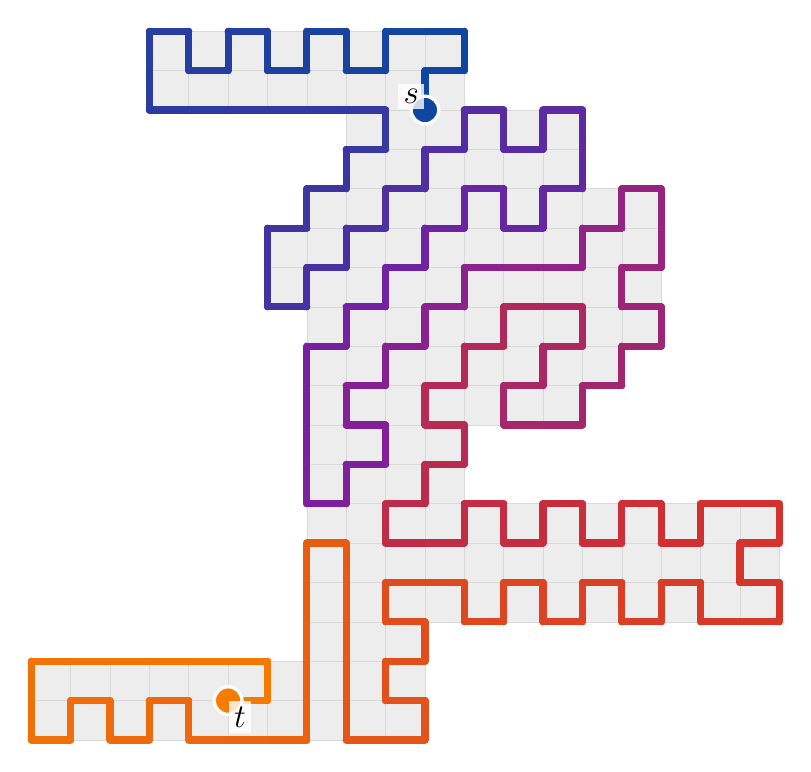
\begin{tikzpicture}[scale=0.5]
\fill[herocell] (-8,-8) rectangle (-7,-7);
\fill[herocell] (-8,-7) rectangle (-7,-6);
\fill[herocell] (-7,-8) rectangle (-6,-7);
\fill[herocell] (-7,-7) rectangle (-6,-6);
\fill[herocell] (-6,-8) rectangle (-5,-7);
\fill[herocell] (-6,-7) rectangle (-5,-6);
\fill[herocell] (-5,-8) rectangle (-4,-7);
\fill[herocell] (-5,-7) rectangle (-4,-6);
\fill[herocell] (-5,8) rectangle (-4,9);
\fill[herocell] (-5,9) rectangle (-4,10);
\fill[herocell] (-4,-8) rectangle (-3,-7);
\fill[herocell] (-4,-7) rectangle (-3,-6);
\fill[herocell] (-4,8) rectangle (-3,9);
\fill[herocell] (-4,9) rectangle (-3,10);
\fill[herocell] (-3,-8) rectangle (-2,-7);
\fill[herocell] (-3,-7) rectangle (-2,-6);
\fill[herocell] (-3,8) rectangle (-2,9);
\fill[herocell] (-3,9) rectangle (-2,10);
\fill[herocell] (-2,-8) rectangle (-1,-7);
\fill[herocell] (-2,-7) rectangle (-1,-6);
\fill[herocell] (-2,3) rectangle (-1,4);
\fill[herocell] (-2,4) rectangle (-1,5);
\fill[herocell] (-2,8) rectangle (-1,9);
\fill[herocell] (-2,9) rectangle (-1,10);
\fill[herocell] (-1,-8) rectangle (0,-7);
\fill[herocell] (-1,-7) rectangle (0,-6);
\fill[herocell] (-1,-6) rectangle (0,-5);
\fill[herocell] (-1,-5) rectangle (0,-4);
\fill[herocell] (-1,-4) rectangle (0,-3);
\fill[herocell] (-1,-3) rectangle (0,-2);
\fill[herocell] (-1,-2) rectangle (0,-1);
\fill[herocell] (-1,-1) rectangle (0,0);
\fill[herocell] (-1,0) rectangle (0,1);
\fill[herocell] (-1,1) rectangle (0,2);
\fill[herocell] (-1,2) rectangle (0,3);
\fill[herocell] (-1,3) rectangle (0,4);
\fill[herocell] (-1,4) rectangle (0,5);
\fill[herocell] (-1,5) rectangle (0,6);
\fill[herocell] (-1,8) rectangle (0,9);
\fill[herocell] (-1,9) rectangle (0,10);
\fill[herocell] (0,-8) rectangle (1,-7);
\fill[herocell] (0,-7) rectangle (1,-6);
\fill[herocell] (0,-6) rectangle (1,-5);
\fill[herocell] (0,-5) rectangle (1,-4);
\fill[herocell] (0,-4) rectangle (1,-3);
\fill[herocell] (0,-3) rectangle (1,-2);
\fill[herocell] (0,-2) rectangle (1,-1);
\fill[herocell] (0,-1) rectangle (1,0);
\fill[herocell] (0,0) rectangle (1,1);
\fill[herocell] (0,1) rectangle (1,2);
\fill[herocell] (0,2) rectangle (1,3);
\fill[herocell] (0,3) rectangle (1,4);
\fill[herocell] (0,4) rectangle (1,5);
\fill[herocell] (0,5) rectangle (1,6);
\fill[herocell] (0,6) rectangle (1,7);
\fill[herocell] (0,7) rectangle (1,8);
\fill[herocell] (0,8) rectangle (1,9);
\fill[herocell] (0,9) rectangle (1,10);
\fill[herocell] (1,-8) rectangle (2,-7);
\fill[herocell] (1,-7) rectangle (2,-6);
\fill[herocell] (1,-6) rectangle (2,-5);
\fill[herocell] (1,-5) rectangle (2,-4);
\fill[herocell] (1,-4) rectangle (2,-3);
\fill[herocell] (1,-3) rectangle (2,-2);
\fill[herocell] (1,-2) rectangle (2,-1);
\fill[herocell] (1,-1) rectangle (2,0);
\fill[herocell] (1,0) rectangle (2,1);
\fill[herocell] (1,1) rectangle (2,2);
\fill[herocell] (1,2) rectangle (2,3);
\fill[herocell] (1,3) rectangle (2,4);
\fill[herocell] (1,4) rectangle (2,5);
\fill[herocell] (1,5) rectangle (2,6);
\fill[herocell] (1,6) rectangle (2,7);
\fill[herocell] (1,7) rectangle (2,8);
\fill[herocell] (1,8) rectangle (2,9);
\fill[herocell] (1,9) rectangle (2,10);
\fill[herocell] (2,-5) rectangle (3,-4);
\fill[herocell] (2,-4) rectangle (3,-3);
\fill[herocell] (2,-3) rectangle (3,-2);
\fill[herocell] (2,-2) rectangle (3,-1);
\fill[herocell] (2,-1) rectangle (3,0);
\fill[herocell] (2,0) rectangle (3,1);
\fill[herocell] (2,1) rectangle (3,2);
\fill[herocell] (2,2) rectangle (3,3);
\fill[herocell] (2,3) rectangle (3,4);
\fill[herocell] (2,4) rectangle (3,5);
\fill[herocell] (2,5) rectangle (3,6);
\fill[herocell] (2,6) rectangle (3,7);
\fill[herocell] (2,7) rectangle (3,8);
\fill[herocell] (2,8) rectangle (3,9);
\fill[herocell] (2,9) rectangle (3,10);
\fill[herocell] (3,-5) rectangle (4,-4);
\fill[herocell] (3,-4) rectangle (4,-3);
\fill[herocell] (3,-3) rectangle (4,-2);
\fill[herocell] (3,0) rectangle (4,1);
\fill[herocell] (3,1) rectangle (4,2);
\fill[herocell] (3,2) rectangle (4,3);
\fill[herocell] (3,3) rectangle (4,4);
\fill[herocell] (3,4) rectangle (4,5);
\fill[herocell] (3,5) rectangle (4,6);
\fill[herocell] (3,6) rectangle (4,7);
\fill[herocell] (3,7) rectangle (4,8);
\fill[herocell] (4,-5) rectangle (5,-4);
\fill[herocell] (4,-4) rectangle (5,-3);
\fill[herocell] (4,-3) rectangle (5,-2);
\fill[herocell] (4,0) rectangle (5,1);
\fill[herocell] (4,1) rectangle (5,2);
\fill[herocell] (4,2) rectangle (5,3);
\fill[herocell] (4,3) rectangle (5,4);
\fill[herocell] (4,4) rectangle (5,5);
\fill[herocell] (4,5) rectangle (5,6);
\fill[herocell] (4,6) rectangle (5,7);
\fill[herocell] (4,7) rectangle (5,8);
\fill[herocell] (5,-5) rectangle (6,-4);
\fill[herocell] (5,-4) rectangle (6,-3);
\fill[herocell] (5,-3) rectangle (6,-2);
\fill[herocell] (5,0) rectangle (6,1);
\fill[herocell] (5,1) rectangle (6,2);
\fill[herocell] (5,2) rectangle (6,3);
\fill[herocell] (5,3) rectangle (6,4);
\fill[herocell] (5,4) rectangle (6,5);
\fill[herocell] (5,5) rectangle (6,6);
\fill[herocell] (5,6) rectangle (6,7);
\fill[herocell] (5,7) rectangle (6,8);
\fill[herocell] (6,-5) rectangle (7,-4);
\fill[herocell] (6,-4) rectangle (7,-3);
\fill[herocell] (6,-3) rectangle (7,-2);
\fill[herocell] (6,1) rectangle (7,2);
\fill[herocell] (6,2) rectangle (7,3);
\fill[herocell] (6,3) rectangle (7,4);
\fill[herocell] (6,4) rectangle (7,5);
\fill[herocell] (6,5) rectangle (7,6);
\fill[herocell] (7,-5) rectangle (8,-4);
\fill[herocell] (7,-4) rectangle (8,-3);
\fill[herocell] (7,-3) rectangle (8,-2);
\fill[herocell] (7,2) rectangle (8,3);
\fill[herocell] (7,3) rectangle (8,4);
\fill[herocell] (7,4) rectangle (8,5);
\fill[herocell] (7,5) rectangle (8,6);
\fill[herocell] (8,-5) rectangle (9,-4);
\fill[herocell] (8,-4) rectangle (9,-3);
\fill[herocell] (8,-3) rectangle (9,-2);
\fill[herocell] (9,-5) rectangle (10,-4);
\fill[herocell] (9,-4) rectangle (10,-3);
\fill[herocell] (9,-3) rectangle (10,-2);
\fill[herocell] (10,-5) rectangle (11,-4);
\fill[herocell] (10,-4) rectangle (11,-3);
\fill[herocell] (10,-3) rectangle (11,-2);
\draw[heroedge] (-8,-8) -- (-7,-8);
\draw[heroedge] (-8,-8) -- (-8,-7);
\draw[heroedge] (-8,-7) -- (-7,-7);
\draw[heroedge] (-8,-7) -- (-8,-6);
\draw[heroedge] (-8,-6) -- (-7,-6);
\draw[heroedge] (-7,-8) -- (-6,-8);
\draw[heroedge] (-7,-8) -- (-7,-7);
\draw[heroedge] (-7,-7) -- (-6,-7);
\draw[heroedge] (-7,-7) -- (-7,-6);
\draw[heroedge] (-7,-6) -- (-6,-6);
\draw[heroedge] (-6,-8) -- (-5,-8);
\draw[heroedge] (-6,-8) -- (-6,-7);
\draw[heroedge] (-6,-7) -- (-5,-7);
\draw[heroedge] (-6,-7) -- (-6,-6);
\draw[heroedge] (-6,-6) -- (-5,-6);
\draw[heroedge] (-5,-8) -- (-4,-8);
\draw[heroedge] (-5,-8) -- (-5,-7);
\draw[heroedge] (-5,-7) -- (-4,-7);
\draw[heroedge] (-5,-7) -- (-5,-6);
\draw[heroedge] (-5,-6) -- (-4,-6);
\draw[heroedge] (-5,8) -- (-4,8);
\draw[heroedge] (-5,8) -- (-5,9);
\draw[heroedge] (-5,9) -- (-4,9);
\draw[heroedge] (-5,9) -- (-5,10);
\draw[heroedge] (-5,10) -- (-4,10);
\draw[heroedge] (-4,-8) -- (-3,-8);
\draw[heroedge] (-4,-8) -- (-4,-7);
\draw[heroedge] (-4,-7) -- (-3,-7);
\draw[heroedge] (-4,-7) -- (-4,-6);
\draw[heroedge] (-4,-6) -- (-3,-6);
\draw[heroedge] (-4,8) -- (-3,8);
\draw[heroedge] (-4,8) -- (-4,9);
\draw[heroedge] (-4,9) -- (-3,9);
\draw[heroedge] (-4,9) -- (-4,10);
\draw[heroedge] (-4,10) -- (-3,10);
\draw[heroedge] (-3,-8) -- (-2,-8);
\draw[heroedge] (-3,-8) -- (-3,-7);
\draw[heroedge] (-3,-7) -- (-2,-7);
\draw[heroedge] (-3,-7) -- (-3,-6);
\draw[heroedge] (-3,-6) -- (-2,-6);
\draw[heroedge] (-3,8) -- (-2,8);
\draw[heroedge] (-3,8) -- (-3,9);
\draw[heroedge] (-3,9) -- (-2,9);
\draw[heroedge] (-3,9) -- (-3,10);
\draw[heroedge] (-3,10) -- (-2,10);
\draw[heroedge] (-2,-8) -- (-1,-8);
\draw[heroedge] (-2,-8) -- (-2,-7);
\draw[heroedge] (-2,-7) -- (-1,-7);
\draw[heroedge] (-2,-7) -- (-2,-6);
\draw[heroedge] (-2,-6) -- (-1,-6);
\draw[heroedge] (-2,3) -- (-1,3);
\draw[heroedge] (-2,3) -- (-2,4);
\draw[heroedge] (-2,4) -- (-1,4);
\draw[heroedge] (-2,4) -- (-2,5);
\draw[heroedge] (-2,5) -- (-1,5);
\draw[heroedge] (-2,8) -- (-1,8);
\draw[heroedge] (-2,8) -- (-2,9);
\draw[heroedge] (-2,9) -- (-1,9);
\draw[heroedge] (-2,9) -- (-2,10);
\draw[heroedge] (-2,10) -- (-1,10);
\draw[heroedge] (-1,-8) -- (0,-8);
\draw[heroedge] (-1,-8) -- (-1,-7);
\draw[heroedge] (-1,-7) -- (0,-7);
\draw[heroedge] (-1,-7) -- (-1,-6);
\draw[heroedge] (-1,-6) -- (0,-6);
\draw[heroedge] (-1,-6) -- (-1,-5);
\draw[heroedge] (-1,-5) -- (0,-5);
\draw[heroedge] (-1,-5) -- (-1,-4);
\draw[heroedge] (-1,-4) -- (0,-4);
\draw[heroedge] (-1,-4) -- (-1,-3);
\draw[heroedge] (-1,-3) -- (0,-3);
\draw[heroedge] (-1,-3) -- (-1,-2);
\draw[heroedge] (-1,-2) -- (0,-2);
\draw[heroedge] (-1,-2) -- (-1,-1);
\draw[heroedge] (-1,-1) -- (0,-1);
\draw[heroedge] (-1,-1) -- (-1,0);
\draw[heroedge] (-1,0) -- (0,0);
\draw[heroedge] (-1,0) -- (-1,1);
\draw[heroedge] (-1,1) -- (0,1);
\draw[heroedge] (-1,1) -- (-1,2);
\draw[heroedge] (-1,2) -- (0,2);
\draw[heroedge] (-1,2) -- (-1,3);
\draw[heroedge] (-1,3) -- (0,3);
\draw[heroedge] (-1,3) -- (-1,4);
\draw[heroedge] (-1,4) -- (0,4);
\draw[heroedge] (-1,4) -- (-1,5);
\draw[heroedge] (-1,5) -- (0,5);
\draw[heroedge] (-1,5) -- (-1,6);
\draw[heroedge] (-1,6) -- (0,6);
\draw[heroedge] (-1,8) -- (0,8);
\draw[heroedge] (-1,8) -- (-1,9);
\draw[heroedge] (-1,9) -- (0,9);
\draw[heroedge] (-1,9) -- (-1,10);
\draw[heroedge] (-1,10) -- (0,10);
\draw[heroedge] (0,-8) -- (1,-8);
\draw[heroedge] (0,-8) -- (0,-7);
\draw[heroedge] (0,-7) -- (1,-7);
\draw[heroedge] (0,-7) -- (0,-6);
\draw[heroedge] (0,-6) -- (1,-6);
\draw[heroedge] (0,-6) -- (0,-5);
\draw[heroedge] (0,-5) -- (1,-5);
\draw[heroedge] (0,-5) -- (0,-4);
\draw[heroedge] (0,-4) -- (1,-4);
\draw[heroedge] (0,-4) -- (0,-3);
\draw[heroedge] (0,-3) -- (1,-3);
\draw[heroedge] (0,-3) -- (0,-2);
\draw[heroedge] (0,-2) -- (1,-2);
\draw[heroedge] (0,-2) -- (0,-1);
\draw[heroedge] (0,-1) -- (1,-1);
\draw[heroedge] (0,-1) -- (0,0);
\draw[heroedge] (0,0) -- (1,0);
\draw[heroedge] (0,0) -- (0,1);
\draw[heroedge] (0,1) -- (1,1);
\draw[heroedge] (0,1) -- (0,2);
\draw[heroedge] (0,2) -- (1,2);
\draw[heroedge] (0,2) -- (0,3);
\draw[heroedge] (0,3) -- (1,3);
\draw[heroedge] (0,3) -- (0,4);
\draw[heroedge] (0,4) -- (1,4);
\draw[heroedge] (0,4) -- (0,5);
\draw[heroedge] (0,5) -- (1,5);
\draw[heroedge] (0,5) -- (0,6);
\draw[heroedge] (0,6) -- (1,6);
\draw[heroedge] (0,6) -- (0,7);
\draw[heroedge] (0,7) -- (1,7);
\draw[heroedge] (0,7) -- (0,8);
\draw[heroedge] (0,8) -- (1,8);
\draw[heroedge] (0,8) -- (0,9);
\draw[heroedge] (0,9) -- (1,9);
\draw[heroedge] (0,9) -- (0,10);
\draw[heroedge] (0,10) -- (1,10);
\draw[heroedge] (1,-8) -- (2,-8);
\draw[heroedge] (1,-8) -- (1,-7);
\draw[heroedge] (1,-7) -- (2,-7);
\draw[heroedge] (1,-7) -- (1,-6);
\draw[heroedge] (1,-6) -- (2,-6);
\draw[heroedge] (1,-6) -- (1,-5);
\draw[heroedge] (1,-5) -- (2,-5);
\draw[heroedge] (1,-5) -- (1,-4);
\draw[heroedge] (1,-4) -- (2,-4);
\draw[heroedge] (1,-4) -- (1,-3);
\draw[heroedge] (1,-3) -- (2,-3);
\draw[heroedge] (1,-3) -- (1,-2);
\draw[heroedge] (1,-2) -- (2,-2);
\draw[heroedge] (1,-2) -- (1,-1);
\draw[heroedge] (1,-1) -- (2,-1);
\draw[heroedge] (1,-1) -- (1,0);
\draw[heroedge] (1,0) -- (2,0);
\draw[heroedge] (1,0) -- (1,1);
\draw[heroedge] (1,1) -- (2,1);
\draw[heroedge] (1,1) -- (1,2);
\draw[heroedge] (1,2) -- (2,2);
\draw[heroedge] (1,2) -- (1,3);
\draw[heroedge] (1,3) -- (2,3);
\draw[heroedge] (1,3) -- (1,4);
\draw[heroedge] (1,4) -- (2,4);
\draw[heroedge] (1,4) -- (1,5);
\draw[heroedge] (1,5) -- (2,5);
\draw[heroedge] (1,5) -- (1,6);
\draw[heroedge] (1,6) -- (2,6);
\draw[heroedge] (1,6) -- (1,7);
\draw[heroedge] (1,7) -- (2,7);
\draw[heroedge] (1,7) -- (1,8);
\draw[heroedge] (1,8) -- (2,8);
\draw[heroedge] (1,8) -- (1,9);
\draw[heroedge] (1,9) -- (2,9);
\draw[heroedge] (1,9) -- (1,10);
\draw[heroedge] (1,10) -- (2,10);
\draw[heroedge] (2,-8) -- (2,-7);
\draw[heroedge] (2,-7) -- (2,-6);
\draw[heroedge] (2,-6) -- (2,-5);
\draw[heroedge] (2,-5) -- (3,-5);
\draw[heroedge] (2,-5) -- (2,-4);
\draw[heroedge] (2,-4) -- (3,-4);
\draw[heroedge] (2,-4) -- (2,-3);
\draw[heroedge] (2,-3) -- (3,-3);
\draw[heroedge] (2,-3) -- (2,-2);
\draw[heroedge] (2,-2) -- (3,-2);
\draw[heroedge] (2,-2) -- (2,-1);
\draw[heroedge] (2,-1) -- (3,-1);
\draw[heroedge] (2,-1) -- (2,0);
\draw[heroedge] (2,0) -- (3,0);
\draw[heroedge] (2,0) -- (2,1);
\draw[heroedge] (2,1) -- (3,1);
\draw[heroedge] (2,1) -- (2,2);
\draw[heroedge] (2,2) -- (3,2);
\draw[heroedge] (2,2) -- (2,3);
\draw[heroedge] (2,3) -- (3,3);
\draw[heroedge] (2,3) -- (2,4);
\draw[heroedge] (2,4) -- (3,4);
\draw[heroedge] (2,4) -- (2,5);
\draw[heroedge] (2,5) -- (3,5);
\draw[heroedge] (2,5) -- (2,6);
\draw[heroedge] (2,6) -- (3,6);
\draw[heroedge] (2,6) -- (2,7);
\draw[heroedge] (2,7) -- (3,7);
\draw[heroedge] (2,7) -- (2,8);
\draw[heroedge] (2,8) -- (3,8);
\draw[heroedge] (2,8) -- (2,9);
\draw[heroedge] (2,9) -- (3,9);
\draw[heroedge] (2,9) -- (2,10);
\draw[heroedge] (2,10) -- (3,10);
\draw[heroedge] (3,-5) -- (4,-5);
\draw[heroedge] (3,-5) -- (3,-4);
\draw[heroedge] (3,-4) -- (4,-4);
\draw[heroedge] (3,-4) -- (3,-3);
\draw[heroedge] (3,-3) -- (4,-3);
\draw[heroedge] (3,-3) -- (3,-2);
\draw[heroedge] (3,-2) -- (4,-2);
\draw[heroedge] (3,-2) -- (3,-1);
\draw[heroedge] (3,-1) -- (3,0);
\draw[heroedge] (3,0) -- (4,0);
\draw[heroedge] (3,0) -- (3,1);
\draw[heroedge] (3,1) -- (4,1);
\draw[heroedge] (3,1) -- (3,2);
\draw[heroedge] (3,2) -- (4,2);
\draw[heroedge] (3,2) -- (3,3);
\draw[heroedge] (3,3) -- (4,3);
\draw[heroedge] (3,3) -- (3,4);
\draw[heroedge] (3,4) -- (4,4);
\draw[heroedge] (3,4) -- (3,5);
\draw[heroedge] (3,5) -- (4,5);
\draw[heroedge] (3,5) -- (3,6);
\draw[heroedge] (3,6) -- (4,6);
\draw[heroedge] (3,6) -- (3,7);
\draw[heroedge] (3,7) -- (4,7);
\draw[heroedge] (3,7) -- (3,8);
\draw[heroedge] (3,8) -- (4,8);
\draw[heroedge] (3,8) -- (3,9);
\draw[heroedge] (3,9) -- (3,10);
\draw[heroedge] (4,-5) -- (5,-5);
\draw[heroedge] (4,-5) -- (4,-4);
\draw[heroedge] (4,-4) -- (5,-4);
\draw[heroedge] (4,-4) -- (4,-3);
\draw[heroedge] (4,-3) -- (5,-3);
\draw[heroedge] (4,-3) -- (4,-2);
\draw[heroedge] (4,-2) -- (5,-2);
\draw[heroedge] (4,0) -- (5,0);
\draw[heroedge] (4,0) -- (4,1);
\draw[heroedge] (4,1) -- (5,1);
\draw[heroedge] (4,1) -- (4,2);
\draw[heroedge] (4,2) -- (5,2);
\draw[heroedge] (4,2) -- (4,3);
\draw[heroedge] (4,3) -- (5,3);
\draw[heroedge] (4,3) -- (4,4);
\draw[heroedge] (4,4) -- (5,4);
\draw[heroedge] (4,4) -- (4,5);
\draw[heroedge] (4,5) -- (5,5);
\draw[heroedge] (4,5) -- (4,6);
\draw[heroedge] (4,6) -- (5,6);
\draw[heroedge] (4,6) -- (4,7);
\draw[heroedge] (4,7) -- (5,7);
\draw[heroedge] (4,7) -- (4,8);
\draw[heroedge] (4,8) -- (5,8);
\draw[heroedge] (5,-5) -- (6,-5);
\draw[heroedge] (5,-5) -- (5,-4);
\draw[heroedge] (5,-4) -- (6,-4);
\draw[heroedge] (5,-4) -- (5,-3);
\draw[heroedge] (5,-3) -- (6,-3);
\draw[heroedge] (5,-3) -- (5,-2);
\draw[heroedge] (5,-2) -- (6,-2);
\draw[heroedge] (5,0) -- (6,0);
\draw[heroedge] (5,0) -- (5,1);
\draw[heroedge] (5,1) -- (6,1);
\draw[heroedge] (5,1) -- (5,2);
\draw[heroedge] (5,2) -- (6,2);
\draw[heroedge] (5,2) -- (5,3);
\draw[heroedge] (5,3) -- (6,3);
\draw[heroedge] (5,3) -- (5,4);
\draw[heroedge] (5,4) -- (6,4);
\draw[heroedge] (5,4) -- (5,5);
\draw[heroedge] (5,5) -- (6,5);
\draw[heroedge] (5,5) -- (5,6);
\draw[heroedge] (5,6) -- (6,6);
\draw[heroedge] (5,6) -- (5,7);
\draw[heroedge] (5,7) -- (6,7);
\draw[heroedge] (5,7) -- (5,8);
\draw[heroedge] (5,8) -- (6,8);
\draw[heroedge] (6,-5) -- (7,-5);
\draw[heroedge] (6,-5) -- (6,-4);
\draw[heroedge] (6,-4) -- (7,-4);
\draw[heroedge] (6,-4) -- (6,-3);
\draw[heroedge] (6,-3) -- (7,-3);
\draw[heroedge] (6,-3) -- (6,-2);
\draw[heroedge] (6,-2) -- (7,-2);
\draw[heroedge] (6,0) -- (6,1);
\draw[heroedge] (6,1) -- (7,1);
\draw[heroedge] (6,1) -- (6,2);
\draw[heroedge] (6,2) -- (7,2);
\draw[heroedge] (6,2) -- (6,3);
\draw[heroedge] (6,3) -- (7,3);
\draw[heroedge] (6,3) -- (6,4);
\draw[heroedge] (6,4) -- (7,4);
\draw[heroedge] (6,4) -- (6,5);
\draw[heroedge] (6,5) -- (7,5);
\draw[heroedge] (6,5) -- (6,6);
\draw[heroedge] (6,6) -- (7,6);
\draw[heroedge] (6,6) -- (6,7);
\draw[heroedge] (6,7) -- (6,8);
\draw[heroedge] (7,-5) -- (8,-5);
\draw[heroedge] (7,-5) -- (7,-4);
\draw[heroedge] (7,-4) -- (8,-4);
\draw[heroedge] (7,-4) -- (7,-3);
\draw[heroedge] (7,-3) -- (8,-3);
\draw[heroedge] (7,-3) -- (7,-2);
\draw[heroedge] (7,-2) -- (8,-2);
\draw[heroedge] (7,1) -- (7,2);
\draw[heroedge] (7,2) -- (8,2);
\draw[heroedge] (7,2) -- (7,3);
\draw[heroedge] (7,3) -- (8,3);
\draw[heroedge] (7,3) -- (7,4);
\draw[heroedge] (7,4) -- (8,4);
\draw[heroedge] (7,4) -- (7,5);
\draw[heroedge] (7,5) -- (8,5);
\draw[heroedge] (7,5) -- (7,6);
\draw[heroedge] (7,6) -- (8,6);
\draw[heroedge] (8,-5) -- (9,-5);
\draw[heroedge] (8,-5) -- (8,-4);
\draw[heroedge] (8,-4) -- (9,-4);
\draw[heroedge] (8,-4) -- (8,-3);
\draw[heroedge] (8,-3) -- (9,-3);
\draw[heroedge] (8,-3) -- (8,-2);
\draw[heroedge] (8,-2) -- (9,-2);
\draw[heroedge] (8,2) -- (8,3);
\draw[heroedge] (8,3) -- (8,4);
\draw[heroedge] (8,4) -- (8,5);
\draw[heroedge] (8,5) -- (8,6);
\draw[heroedge] (9,-5) -- (10,-5);
\draw[heroedge] (9,-5) -- (9,-4);
\draw[heroedge] (9,-4) -- (10,-4);
\draw[heroedge] (9,-4) -- (9,-3);
\draw[heroedge] (9,-3) -- (10,-3);
\draw[heroedge] (9,-3) -- (9,-2);
\draw[heroedge] (9,-2) -- (10,-2);
\draw[heroedge] (10,-5) -- (11,-5);
\draw[heroedge] (10,-5) -- (10,-4);
\draw[heroedge] (10,-4) -- (11,-4);
\draw[heroedge] (10,-4) -- (10,-3);
\draw[heroedge] (10,-3) -- (11,-3);
\draw[heroedge] (10,-3) -- (10,-2);
\draw[heroedge] (10,-2) -- (11,-2);
\draw[heroedge] (11,-5) -- (11,-4);
\draw[heroedge] (11,-4) -- (11,-3);
\draw[heroedge] (11,-3) -- (11,-2);
\node[heropt] at (-8,-8) {};
\node[heropt] at (-8,-7) {};
\node[heropt] at (-8,-6) {};
\node[heropt] at (-7,-8) {};
\node[heropt] at (-7,-7) {};
\node[heropt] at (-7,-6) {};
\node[heropt] at (-6,-8) {};
\node[heropt] at (-6,-7) {};
\node[heropt] at (-6,-6) {};
\node[heropt] at (-5,-8) {};
\node[heropt] at (-5,-7) {};
\node[heropt] at (-5,-6) {};
\node[heropt] at (-5,8) {};
\node[heropt] at (-5,9) {};
\node[heropt] at (-5,10) {};
\node[heropt] at (-4,-8) {};
\node[heropt] at (-4,-7) {};
\node[heropt] at (-4,-6) {};
\node[heropt] at (-4,8) {};
\node[heropt] at (-4,9) {};
\node[heropt] at (-4,10) {};
\node[heropt] at (-3,-8) {};
\node[heropt] at (-3,-7) {};
\node[heropt] at (-3,-6) {};
\node[heropt] at (-3,8) {};
\node[heropt] at (-3,9) {};
\node[heropt] at (-3,10) {};
\node[heropt] at (-2,-8) {};
\node[heropt] at (-2,-7) {};
\node[heropt] at (-2,-6) {};
\node[heropt] at (-2,3) {};
\node[heropt] at (-2,4) {};
\node[heropt] at (-2,5) {};
\node[heropt] at (-2,8) {};
\node[heropt] at (-2,9) {};
\node[heropt] at (-2,10) {};
\node[heropt] at (-1,-8) {};
\node[heropt] at (-1,-7) {};
\node[heropt] at (-1,-6) {};
\node[heropt] at (-1,-5) {};
\node[heropt] at (-1,-4) {};
\node[heropt] at (-1,-3) {};
\node[heropt] at (-1,-2) {};
\node[heropt] at (-1,-1) {};
\node[heropt] at (-1,0) {};
\node[heropt] at (-1,1) {};
\node[heropt] at (-1,2) {};
\node[heropt] at (-1,3) {};
\node[heropt] at (-1,4) {};
\node[heropt] at (-1,5) {};
\node[heropt] at (-1,6) {};
\node[heropt] at (-1,8) {};
\node[heropt] at (-1,9) {};
\node[heropt] at (-1,10) {};
\node[heropt] at (0,-8) {};
\node[heropt] at (0,-7) {};
\node[heropt] at (0,-6) {};
\node[heropt] at (0,-5) {};
\node[heropt] at (0,-4) {};
\node[heropt] at (0,-3) {};
\node[heropt] at (0,-2) {};
\node[heropt] at (0,-1) {};
\node[heropt] at (0,0) {};
\node[heropt] at (0,1) {};
\node[heropt] at (0,2) {};
\node[heropt] at (0,3) {};
\node[heropt] at (0,4) {};
\node[heropt] at (0,5) {};
\node[heropt] at (0,6) {};
\node[heropt] at (0,7) {};
\node[heropt] at (0,8) {};
\node[heropt] at (0,9) {};
\node[heropt] at (0,10) {};
\node[heropt] at (1,-8) {};
\node[heropt] at (1,-7) {};
\node[heropt] at (1,-6) {};
\node[heropt] at (1,-5) {};
\node[heropt] at (1,-4) {};
\node[heropt] at (1,-3) {};
\node[heropt] at (1,-2) {};
\node[heropt] at (1,-1) {};
\node[heropt] at (1,0) {};
\node[heropt] at (1,1) {};
\node[heropt] at (1,2) {};
\node[heropt] at (1,3) {};
\node[heropt] at (1,4) {};
\node[heropt] at (1,5) {};
\node[heropt] at (1,6) {};
\node[heropt] at (1,7) {};
\node[heropt] at (1,8) {};
\node[heropt] at (1,9) {};
\node[heropt] at (1,10) {};
\node[heropt] at (2,-8) {};
\node[heropt] at (2,-7) {};
\node[heropt] at (2,-6) {};
\node[heropt] at (2,-5) {};
\node[heropt] at (2,-4) {};
\node[heropt] at (2,-3) {};
\node[heropt] at (2,-2) {};
\node[heropt] at (2,-1) {};
\node[heropt] at (2,0) {};
\node[heropt] at (2,1) {};
\node[heropt] at (2,2) {};
\node[heropt] at (2,3) {};
\node[heropt] at (2,4) {};
\node[heropt] at (2,5) {};
\node[heropt] at (2,6) {};
\node[heropt] at (2,7) {};
\node[heropt] at (2,8) {};
\node[heropt] at (2,9) {};
\node[heropt] at (2,10) {};
\node[heropt] at (3,-5) {};
\node[heropt] at (3,-4) {};
\node[heropt] at (3,-3) {};
\node[heropt] at (3,-2) {};
\node[heropt] at (3,-1) {};
\node[heropt] at (3,0) {};
\node[heropt] at (3,1) {};
\node[heropt] at (3,2) {};
\node[heropt] at (3,3) {};
\node[heropt] at (3,4) {};
\node[heropt] at (3,5) {};
\node[heropt] at (3,6) {};
\node[heropt] at (3,7) {};
\node[heropt] at (3,8) {};
\node[heropt] at (3,9) {};
\node[heropt] at (3,10) {};
\node[heropt] at (4,-5) {};
\node[heropt] at (4,-4) {};
\node[heropt] at (4,-3) {};
\node[heropt] at (4,-2) {};
\node[heropt] at (4,0) {};
\node[heropt] at (4,1) {};
\node[heropt] at (4,2) {};
\node[heropt] at (4,3) {};
\node[heropt] at (4,4) {};
\node[heropt] at (4,5) {};
\node[heropt] at (4,6) {};
\node[heropt] at (4,7) {};
\node[heropt] at (4,8) {};
\node[heropt] at (5,-5) {};
\node[heropt] at (5,-4) {};
\node[heropt] at (5,-3) {};
\node[heropt] at (5,-2) {};
\node[heropt] at (5,0) {};
\node[heropt] at (5,1) {};
\node[heropt] at (5,2) {};
\node[heropt] at (5,3) {};
\node[heropt] at (5,4) {};
\node[heropt] at (5,5) {};
\node[heropt] at (5,6) {};
\node[heropt] at (5,7) {};
\node[heropt] at (5,8) {};
\node[heropt] at (6,-5) {};
\node[heropt] at (6,-4) {};
\node[heropt] at (6,-3) {};
\node[heropt] at (6,-2) {};
\node[heropt] at (6,0) {};
\node[heropt] at (6,1) {};
\node[heropt] at (6,2) {};
\node[heropt] at (6,3) {};
\node[heropt] at (6,4) {};
\node[heropt] at (6,5) {};
\node[heropt] at (6,6) {};
\node[heropt] at (6,7) {};
\node[heropt] at (6,8) {};
\node[heropt] at (7,-5) {};
\node[heropt] at (7,-4) {};
\node[heropt] at (7,-3) {};
\node[heropt] at (7,-2) {};
\node[heropt] at (7,1) {};
\node[heropt] at (7,2) {};
\node[heropt] at (7,3) {};
\node[heropt] at (7,4) {};
\node[heropt] at (7,5) {};
\node[heropt] at (7,6) {};
\node[heropt] at (8,-5) {};
\node[heropt] at (8,-4) {};
\node[heropt] at (8,-3) {};
\node[heropt] at (8,-2) {};
\node[heropt] at (8,2) {};
\node[heropt] at (8,3) {};
\node[heropt] at (8,4) {};
\node[heropt] at (8,5) {};
\node[heropt] at (8,6) {};
\node[heropt] at (9,-5) {};
\node[heropt] at (9,-4) {};
\node[heropt] at (9,-3) {};
\node[heropt] at (9,-2) {};
\node[heropt] at (10,-5) {};
\node[heropt] at (10,-4) {};
\node[heropt] at (10,-3) {};
\node[heropt] at (10,-2) {};
\node[heropt] at (11,-5) {};
\node[heropt] at (11,-4) {};
\node[heropt] at (11,-3) {};
\node[heropt] at (11,-2) {};
\draw[heropath,color={rgb,255:red,13;green,71;blue,161}] (2,8) -- (2,9);
\draw[heropath,color={rgb,255:red,15;green,70;blue,161}] (2,9) -- (3,9);
\draw[heropath,color={rgb,255:red,16;green,70;blue,161}] (3,9) -- (3,10);
\draw[heropath,color={rgb,255:red,18;green,69;blue,161}] (3,10) -- (2,10);
\draw[heropath,color={rgb,255:red,20;green,69;blue,161}] (2,10) -- (1,10);
\draw[heropath,color={rgb,255:red,21;green,68;blue,161}] (1,10) -- (1,9);
\draw[heropath,color={rgb,255:red,23;green,67;blue,161}] (1,9) -- (0,9);
\draw[heropath,color={rgb,255:red,25;green,67;blue,161}] (0,9) -- (0,10);
\draw[heropath,color={rgb,255:red,26;green,66;blue,161}] (0,10) -- (-1,10);
\draw[heropath,color={rgb,255:red,28;green,65;blue,161}] (-1,10) -- (-1,9);
\draw[heropath,color={rgb,255:red,30;green,65;blue,161}] (-1,9) -- (-2,9);
\draw[heropath,color={rgb,255:red,32;green,64;blue,161}] (-2,9) -- (-2,10);
\draw[heropath,color={rgb,255:red,33;green,64;blue,161}] (-2,10) -- (-3,10);
\draw[heropath,color={rgb,255:red,35;green,63;blue,161}] (-3,10) -- (-3,9);
\draw[heropath,color={rgb,255:red,37;green,62;blue,161}] (-3,9) -- (-4,9);
\draw[heropath,color={rgb,255:red,38;green,62;blue,161}] (-4,9) -- (-4,10);
\draw[heropath,color={rgb,255:red,40;green,61;blue,161}] (-4,10) -- (-5,10);
\draw[heropath,color={rgb,255:red,42;green,61;blue,161}] (-5,10) -- (-5,9);
\draw[heropath,color={rgb,255:red,43;green,60;blue,161}] (-5,9) -- (-5,8);
\draw[heropath,color={rgb,255:red,45;green,59;blue,161}] (-5,8) -- (-4,8);
\draw[heropath,color={rgb,255:red,47;green,59;blue,161}] (-4,8) -- (-3,8);
\draw[heropath,color={rgb,255:red,48;green,58;blue,161}] (-3,8) -- (-2,8);
\draw[heropath,color={rgb,255:red,50;green,58;blue,161}] (-2,8) -- (-1,8);
\draw[heropath,color={rgb,255:red,52;green,57;blue,161}] (-1,8) -- (0,8);
\draw[heropath,color={rgb,255:red,53;green,56;blue,161}] (0,8) -- (1,8);
\draw[heropath,color={rgb,255:red,55;green,56;blue,161}] (1,8) -- (1,7);
\draw[heropath,color={rgb,255:red,57;green,55;blue,161}] (1,7) -- (0,7);
\draw[heropath,color={rgb,255:red,58;green,54;blue,161}] (0,7) -- (0,6);
\draw[heropath,color={rgb,255:red,60;green,54;blue,161}] (0,6) -- (-1,6);
\draw[heropath,color={rgb,255:red,62;green,53;blue,161}] (-1,6) -- (-1,5);
\draw[heropath,color={rgb,255:red,64;green,53;blue,161}] (-1,5) -- (-2,5);
\draw[heropath,color={rgb,255:red,65;green,52;blue,161}] (-2,5) -- (-2,4);
\draw[heropath,color={rgb,255:red,67;green,51;blue,161}] (-2,4) -- (-2,3);
\draw[heropath,color={rgb,255:red,69;green,51;blue,162}] (-2,3) -- (-1,3);
\draw[heropath,color={rgb,255:red,70;green,50;blue,162}] (-1,3) -- (-1,4);
\draw[heropath,color={rgb,255:red,72;green,50;blue,162}] (-1,4) -- (0,4);
\draw[heropath,color={rgb,255:red,74;green,49;blue,162}] (0,4) -- (0,5);
\draw[heropath,color={rgb,255:red,75;green,48;blue,162}] (0,5) -- (1,5);
\draw[heropath,color={rgb,255:red,77;green,48;blue,162}] (1,5) -- (1,6);
\draw[heropath,color={rgb,255:red,79;green,47;blue,162}] (1,6) -- (2,6);
\draw[heropath,color={rgb,255:red,80;green,47;blue,162}] (2,6) -- (2,7);
\draw[heropath,color={rgb,255:red,82;green,46;blue,162}] (2,7) -- (3,7);
\draw[heropath,color={rgb,255:red,84;green,45;blue,162}] (3,7) -- (3,8);
\draw[heropath,color={rgb,255:red,85;green,45;blue,162}] (3,8) -- (4,8);
\draw[heropath,color={rgb,255:red,87;green,44;blue,162}] (4,8) -- (4,7);
\draw[heropath,color={rgb,255:red,89;green,43;blue,162}] (4,7) -- (5,7);
\draw[heropath,color={rgb,255:red,90;green,43;blue,162}] (5,7) -- (5,8);
\draw[heropath,color={rgb,255:red,92;green,42;blue,162}] (5,8) -- (6,8);
\draw[heropath,color={rgb,255:red,94;green,42;blue,162}] (6,8) -- (6,7);
\draw[heropath,color={rgb,255:red,96;green,41;blue,162}] (6,7) -- (6,6);
\draw[heropath,color={rgb,255:red,97;green,40;blue,162}] (6,6) -- (5,6);
\draw[heropath,color={rgb,255:red,99;green,40;blue,162}] (5,6) -- (5,5);
\draw[heropath,color={rgb,255:red,101;green,39;blue,162}] (5,5) -- (4,5);
\draw[heropath,color={rgb,255:red,102;green,39;blue,162}] (4,5) -- (4,6);
\draw[heropath,color={rgb,255:red,104;green,38;blue,162}] (4,6) -- (3,6);
\draw[heropath,color={rgb,255:red,106;green,37;blue,162}] (3,6) -- (3,5);
\draw[heropath,color={rgb,255:red,107;green,37;blue,162}] (3,5) -- (2,5);
\draw[heropath,color={rgb,255:red,109;green,36;blue,162}] (2,5) -- (2,4);
\draw[heropath,color={rgb,255:red,111;green,35;blue,162}] (2,4) -- (1,4);
\draw[heropath,color={rgb,255:red,112;green,35;blue,162}] (1,4) -- (1,3);
\draw[heropath,color={rgb,255:red,114;green,34;blue,162}] (1,3) -- (0,3);
\draw[heropath,color={rgb,255:red,116;green,34;blue,162}] (0,3) -- (0,2);
\draw[heropath,color={rgb,255:red,117;green,33;blue,162}] (0,2) -- (-1,2);
\draw[heropath,color={rgb,255:red,119;green,32;blue,162}] (-1,2) -- (-1,1);
\draw[heropath,color={rgb,255:red,121;green,32;blue,162}] (-1,1) -- (-1,0);
\draw[heropath,color={rgb,255:red,122;green,31;blue,162}] (-1,0) -- (-1,-1);
\draw[heropath,color={rgb,255:red,124;green,31;blue,161}] (-1,-1) -- (-1,-2);
\draw[heropath,color={rgb,255:red,125;green,31;blue,159}] (-1,-2) -- (0,-2);
\draw[heropath,color={rgb,255:red,127;green,32;blue,157}] (0,-2) -- (0,-1);
\draw[heropath,color={rgb,255:red,128;green,32;blue,156}] (0,-1) -- (1,-1);
\draw[heropath,color={rgb,255:red,129;green,32;blue,154}] (1,-1) -- (1,0);
\draw[heropath,color={rgb,255:red,131;green,32;blue,152}] (1,0) -- (0,0);
\draw[heropath,color={rgb,255:red,132;green,33;blue,150}] (0,0) -- (0,1);
\draw[heropath,color={rgb,255:red,133;green,33;blue,149}] (0,1) -- (1,1);
\draw[heropath,color={rgb,255:red,135;green,33;blue,147}] (1,1) -- (1,2);
\draw[heropath,color={rgb,255:red,136;green,33;blue,145}] (1,2) -- (2,2);
\draw[heropath,color={rgb,255:red,137;green,34;blue,143}] (2,2) -- (2,3);
\draw[heropath,color={rgb,255:red,139;green,34;blue,141}] (2,3) -- (3,3);
\draw[heropath,color={rgb,255:red,140;green,34;blue,140}] (3,3) -- (3,4);
\draw[heropath,color={rgb,255:red,141;green,34;blue,138}] (3,4) -- (4,4);
\draw[heropath,color={rgb,255:red,143;green,35;blue,136}] (4,4) -- (5,4);
\draw[heropath,color={rgb,255:red,144;green,35;blue,134}] (5,4) -- (6,4);
\draw[heropath,color={rgb,255:red,145;green,35;blue,133}] (6,4) -- (6,5);
\draw[heropath,color={rgb,255:red,147;green,35;blue,131}] (6,5) -- (7,5);
\draw[heropath,color={rgb,255:red,148;green,36;blue,129}] (7,5) -- (7,6);
\draw[heropath,color={rgb,255:red,149;green,36;blue,127}] (7,6) -- (8,6);
\draw[heropath,color={rgb,255:red,151;green,36;blue,126}] (8,6) -- (8,5);
\draw[heropath,color={rgb,255:red,152;green,36;blue,124}] (8,5) -- (8,4);
\draw[heropath,color={rgb,255:red,154;green,37;blue,122}] (8,4) -- (7,4);
\draw[heropath,color={rgb,255:red,155;green,37;blue,120}] (7,4) -- (7,3);
\draw[heropath,color={rgb,255:red,156;green,37;blue,119}] (7,3) -- (8,3);
\draw[heropath,color={rgb,255:red,158;green,37;blue,117}] (8,3) -- (8,2);
\draw[heropath,color={rgb,255:red,159;green,38;blue,115}] (8,2) -- (7,2);
\draw[heropath,color={rgb,255:red,160;green,38;blue,113}] (7,2) -- (7,1);
\draw[heropath,color={rgb,255:red,162;green,38;blue,112}] (7,1) -- (6,1);
\draw[heropath,color={rgb,255:red,163;green,38;blue,110}] (6,1) -- (6,0);
\draw[heropath,color={rgb,255:red,164;green,39;blue,108}] (6,0) -- (5,0);
\draw[heropath,color={rgb,255:red,166;green,39;blue,106}] (5,0) -- (4,0);
\draw[heropath,color={rgb,255:red,167;green,39;blue,104}] (4,0) -- (4,1);
\draw[heropath,color={rgb,255:red,168;green,39;blue,103}] (4,1) -- (5,1);
\draw[heropath,color={rgb,255:red,170;green,39;blue,101}] (5,1) -- (5,2);
\draw[heropath,color={rgb,255:red,171;green,40;blue,99}] (5,2) -- (6,2);
\draw[heropath,color={rgb,255:red,172;green,40;blue,97}] (6,2) -- (6,3);
\draw[heropath,color={rgb,255:red,174;green,40;blue,96}] (6,3) -- (5,3);
\draw[heropath,color={rgb,255:red,175;green,40;blue,94}] (5,3) -- (4,3);
\draw[heropath,color={rgb,255:red,176;green,41;blue,92}] (4,3) -- (4,2);
\draw[heropath,color={rgb,255:red,178;green,41;blue,90}] (4,2) -- (3,2);
\draw[heropath,color={rgb,255:red,179;green,41;blue,89}] (3,2) -- (3,1);
\draw[heropath,color={rgb,255:red,180;green,41;blue,87}] (3,1) -- (2,1);
\draw[heropath,color={rgb,255:red,182;green,42;blue,85}] (2,1) -- (2,0);
\draw[heropath,color={rgb,255:red,183;green,42;blue,83}] (2,0) -- (3,0);
\draw[heropath,color={rgb,255:red,185;green,42;blue,82}] (3,0) -- (3,-1);
\draw[heropath,color={rgb,255:red,186;green,42;blue,80}] (3,-1) -- (2,-1);
\draw[heropath,color={rgb,255:red,187;green,43;blue,78}] (2,-1) -- (2,-2);
\draw[heropath,color={rgb,255:red,189;green,43;blue,76}] (2,-2) -- (1,-2);
\draw[heropath,color={rgb,255:red,190;green,43;blue,75}] (1,-2) -- (1,-3);
\draw[heropath,color={rgb,255:red,191;green,43;blue,73}] (1,-3) -- (2,-3);
\draw[heropath,color={rgb,255:red,193;green,44;blue,71}] (2,-3) -- (3,-3);
\draw[heropath,color={rgb,255:red,194;green,44;blue,69}] (3,-3) -- (3,-2);
\draw[heropath,color={rgb,255:red,195;green,44;blue,68}] (3,-2) -- (4,-2);
\draw[heropath,color={rgb,255:red,197;green,44;blue,66}] (4,-2) -- (4,-3);
\draw[heropath,color={rgb,255:red,198;green,45;blue,64}] (4,-3) -- (5,-3);
\draw[heropath,color={rgb,255:red,199;green,45;blue,62}] (5,-3) -- (5,-2);
\draw[heropath,color={rgb,255:red,201;green,45;blue,60}] (5,-2) -- (6,-2);
\draw[heropath,color={rgb,255:red,202;green,45;blue,59}] (6,-2) -- (6,-3);
\draw[heropath,color={rgb,255:red,203;green,46;blue,57}] (6,-3) -- (7,-3);
\draw[heropath,color={rgb,255:red,205;green,46;blue,55}] (7,-3) -- (7,-2);
\draw[heropath,color={rgb,255:red,206;green,46;blue,53}] (7,-2) -- (8,-2);
\draw[heropath,color={rgb,255:red,207;green,46;blue,52}] (8,-2) -- (8,-3);
\draw[heropath,color={rgb,255:red,209;green,47;blue,50}] (8,-3) -- (9,-3);
\draw[heropath,color={rgb,255:red,210;green,47;blue,48}] (9,-3) -- (9,-2);
\draw[heropath,color={rgb,255:red,211;green,47;blue,47}] (9,-2) -- (10,-2);
\draw[heropath,color={rgb,255:red,212;green,49;blue,46}] (10,-2) -- (11,-2);
\draw[heropath,color={rgb,255:red,212;green,50;blue,45}] (11,-2) -- (11,-3);
\draw[heropath,color={rgb,255:red,213;green,51;blue,45}] (11,-3) -- (10,-3);
\draw[heropath,color={rgb,255:red,213;green,52;blue,44}] (10,-3) -- (10,-4);
\draw[heropath,color={rgb,255:red,214;green,53;blue,43}] (10,-4) -- (11,-4);
\draw[heropath,color={rgb,255:red,214;green,54;blue,42}] (11,-4) -- (11,-5);
\draw[heropath,color={rgb,255:red,215;green,56;blue,42}] (11,-5) -- (10,-5);
\draw[heropath,color={rgb,255:red,215;green,57;blue,41}] (10,-5) -- (9,-5);
\draw[heropath,color={rgb,255:red,216;green,58;blue,40}] (9,-5) -- (9,-4);
\draw[heropath,color={rgb,255:red,216;green,59;blue,40}] (9,-4) -- (8,-4);
\draw[heropath,color={rgb,255:red,217;green,60;blue,39}] (8,-4) -- (8,-5);
\draw[heropath,color={rgb,255:red,217;green,62;blue,38}] (8,-5) -- (7,-5);
\draw[heropath,color={rgb,255:red,218;green,63;blue,37}] (7,-5) -- (7,-4);
\draw[heropath,color={rgb,255:red,218;green,64;blue,37}] (7,-4) -- (6,-4);
\draw[heropath,color={rgb,255:red,219;green,65;blue,36}] (6,-4) -- (6,-5);
\draw[heropath,color={rgb,255:red,220;green,66;blue,35}] (6,-5) -- (5,-5);
\draw[heropath,color={rgb,255:red,220;green,67;blue,35}] (5,-5) -- (5,-4);
\draw[heropath,color={rgb,255:red,221;green,69;blue,34}] (5,-4) -- (4,-4);
\draw[heropath,color={rgb,255:red,221;green,70;blue,33}] (4,-4) -- (4,-5);
\draw[heropath,color={rgb,255:red,222;green,71;blue,32}] (4,-5) -- (3,-5);
\draw[heropath,color={rgb,255:red,222;green,72;blue,32}] (3,-5) -- (3,-4);
\draw[heropath,color={rgb,255:red,223;green,73;blue,31}] (3,-4) -- (2,-4);
\draw[heropath,color={rgb,255:red,223;green,74;blue,30}] (2,-4) -- (1,-4);
\draw[heropath,color={rgb,255:red,224;green,76;blue,29}] (1,-4) -- (1,-5);
\draw[heropath,color={rgb,255:red,224;green,77;blue,29}] (1,-5) -- (2,-5);
\draw[heropath,color={rgb,255:red,225;green,78;blue,28}] (2,-5) -- (2,-6);
\draw[heropath,color={rgb,255:red,225;green,79;blue,27}] (2,-6) -- (1,-6);
\draw[heropath,color={rgb,255:red,226;green,80;blue,27}] (1,-6) -- (1,-7);
\draw[heropath,color={rgb,255:red,226;green,82;blue,26}] (1,-7) -- (2,-7);
\draw[heropath,color={rgb,255:red,227;green,83;blue,25}] (2,-7) -- (2,-8);
\draw[heropath,color={rgb,255:red,227;green,84;blue,24}] (2,-8) -- (1,-8);
\draw[heropath,color={rgb,255:red,228;green,85;blue,24}] (1,-8) -- (0,-8);
\draw[heropath,color={rgb,255:red,228;green,86;blue,23}] (0,-8) -- (0,-7);
\draw[heropath,color={rgb,255:red,229;green,87;blue,22}] (0,-7) -- (0,-6);
\draw[heropath,color={rgb,255:red,229;green,89;blue,22}] (0,-6) -- (0,-5);
\draw[heropath,color={rgb,255:red,230;green,90;blue,21}] (0,-5) -- (0,-4);
\draw[heropath,color={rgb,255:red,230;green,91;blue,20}] (0,-4) -- (0,-3);
\draw[heropath,color={rgb,255:red,231;green,92;blue,19}] (0,-3) -- (-1,-3);
\draw[heropath,color={rgb,255:red,231;green,93;blue,19}] (-1,-3) -- (-1,-4);
\draw[heropath,color={rgb,255:red,232;green,95;blue,18}] (-1,-4) -- (-1,-5);
\draw[heropath,color={rgb,255:red,233;green,96;blue,17}] (-1,-5) -- (-1,-6);
\draw[heropath,color={rgb,255:red,233;green,97;blue,17}] (-1,-6) -- (-1,-7);
\draw[heropath,color={rgb,255:red,234;green,98;blue,16}] (-1,-7) -- (-1,-8);
\draw[heropath,color={rgb,255:red,234;green,99;blue,15}] (-1,-8) -- (-2,-8);
\draw[heropath,color={rgb,255:red,235;green,100;blue,14}] (-2,-8) -- (-3,-8);
\draw[heropath,color={rgb,255:red,235;green,102;blue,14}] (-3,-8) -- (-4,-8);
\draw[heropath,color={rgb,255:red,236;green,103;blue,13}] (-4,-8) -- (-4,-7);
\draw[heropath,color={rgb,255:red,236;green,104;blue,12}] (-4,-7) -- (-5,-7);
\draw[heropath,color={rgb,255:red,237;green,105;blue,12}] (-5,-7) -- (-5,-8);
\draw[heropath,color={rgb,255:red,237;green,106;blue,11}] (-5,-8) -- (-6,-8);
\draw[heropath,color={rgb,255:red,238;green,108;blue,10}] (-6,-8) -- (-6,-7);
\draw[heropath,color={rgb,255:red,238;green,109;blue,9}] (-6,-7) -- (-7,-7);
\draw[heropath,color={rgb,255:red,239;green,110;blue,9}] (-7,-7) -- (-7,-8);
\draw[heropath,color={rgb,255:red,239;green,111;blue,8}] (-7,-8) -- (-8,-8);
\draw[heropath,color={rgb,255:red,240;green,112;blue,7}] (-8,-8) -- (-8,-7);
\draw[heropath,color={rgb,255:red,240;green,113;blue,6}] (-8,-7) -- (-8,-6);
\draw[heropath,color={rgb,255:red,241;green,115;blue,6}] (-8,-6) -- (-7,-6);
\draw[heropath,color={rgb,255:red,241;green,116;blue,5}] (-7,-6) -- (-6,-6);
\draw[heropath,color={rgb,255:red,242;green,117;blue,4}] (-6,-6) -- (-5,-6);
\draw[heropath,color={rgb,255:red,242;green,118;blue,4}] (-5,-6) -- (-4,-6);
\draw[heropath,color={rgb,255:red,243;green,119;blue,3}] (-4,-6) -- (-3,-6);
\draw[heropath,color={rgb,255:red,243;green,120;blue,2}] (-3,-6) -- (-2,-6);
\draw[heropath,color={rgb,255:red,244;green,122;blue,1}] (-2,-6) -- (-2,-7);
\draw[heropath,color={rgb,255:red,244;green,123;blue,1}] (-2,-7) -- (-3,-7);
\node[heroend,fill={rgb,255:red,13;green,71;blue,161}] at (2,8) {};
\node[heroend,fill={rgb,255:red,245;green,124;blue,0}] at (-3,-7) {};
\node[herolab,above left] at (2,8) {$s$};
\node[herolab,below right] at (-3,-7) {$t$};
\end{tikzpicture}

\caption{A Hamiltonian path from $s$ to $t$ on a solid grid graph with $197$ points, found by the
algorithm of this paper.
The path is coloured along its length, from blue at $s$ through purple and red to orange at $t$, so
the order in which it visits the regions of the shape can be read off the colour.
Both endpoints are inner, so the run goes through the two-hole case (\cref{sec:two}).
The shape was made by gluing rotated copies
of rectangles, L, T, U and plus shapes, staircases and discs with arms at least $3$ points wide.}
\label{fig:hero}
\end{figure}

\paragraph{Problem.}
A \emph{grid graph} is given by a finite set $V\subset\Z^2$ of lattice points.
Its edges are the unit segments between two points of $V$.
A \emph{Hamiltonian $s$--$t$ path} is a path through every point of $V$ exactly once, from $s$ to $t$.
For general grid graphs, deciding whether such a path exists is NP-complete~\cite{itai1982}.
A grid graph is \emph{solid} when it has no holes (\cref{def:solid}).
Umans and Lenhart gave a polynomial algorithm for Hamiltonian \emph{cycles} in solid grid
graphs~\cite{umans1997}.
Sheffield gave a second polynomial algorithm for the cycle problem based on height
functions~\cite{sheffield2000}.

\paragraph{Result.}
\begin{theorem}[\lean{decideHamPath\_main}, \lean{HPFinal.lean}]
\label{thm:main}
Let $V\subset\Z^2$ be finite and solid, and let $s\neq t$ be points of $V$.
Then $\lean{decideHamPath}\ V\ s\ t=\lean{true}$ if and only if there is an edge set $H$ of the grid graph
on $V$ with degree $1$ at $s$ and $t$, degree $2$ at every other point, and one connected component.
The cost function $\lean{decideHamPathCost}\ V\ s\ t$ is at most $5\,220\,000\,(|V|+3)^6$.
\end{theorem}

An edge set with these degrees and one component is exactly a Hamiltonian $s$--$t$ path.
The proof assembles the four cases of \cref{tab:cases} and is given there.
The Lean proof uses only the axioms \lean{propext}, \lean{Classical.choice} and \lean{Quot.sound}.

\paragraph{Cost model.}
Running time is stated through explicit cost functions written beside each algorithm in Lean.
Each test is charged by the cost of its evaluation, and each loop is charged for every iteration.
Primitive operations on finite sets (membership, insertion, a cell flip) are charged a constant.
The bound is proved for these functions, not for a machine model.
The correspondence between an algorithm and its cost function is checked by reading the two
definitions side by side.
The constant $5\,220\,000$ is $208$ final tests of the deletion walks (\cref{sec:time}) times the
constant $25\,000$ of one final test, plus the walks' own work.

\paragraph{Prior work in brief.}
Itai, Papadimitriou and Szwarcfiter posed the solid case~\cite{itai1982}.
The Hamiltonian path problem in solid grid graphs is listed as open by
Keshavarz-Kohjerdi~\cite{kk2011} and by Keshavarz-Kohjerdi and Bagheri~\cite{kkb2016c}.
The introduction of Sheffield's paper~\cite{sheffield2000} contains the sentence
``Similar results hold for Hamiltonian paths with fixed endpoints and for other gridlike families of
graphs embedded in $n$-holed tori.''
The present work gives a written proof of the path case and checks it in Lean.
\Cref{app:prior} discusses prior work and novelty in detail.

\paragraph{Contributions.}
\begin{enumerate}
\item \emph{Chained rows}, which complete the count for a stuck phase, and a locally checkable
  certificate for the ``no'' answer (\cref{sec:sheffield}).
\item Phantom endpoints, which move a degree-one endpoint off the vertex set, and a two-phantom
  core under a distance condition (\cref{sec:phantom}).
\item Bounded deletion walks that reach the distance condition (\cref{sec:walk}).
\item For an endpoint with all eight king neighbours present, a hole whose defect is a
  \emph{vortex}, a slit height, and a potential that rules out closed climbs
  (\cref{sec:vortex,sec:two}).
\item Flip classes relative to the deleted endpoints, with a class search by relaxation
  (\cref{sec:classes}).
\item A complete Lean~4 formalization of correctness and a polynomial bound (\cref{sec:lean}).
\end{enumerate}

% =====================================================================
\section{Overview}
\label{sec:overview}

This section explains how the algorithm is put together and why each part is there, before any
definitions.
Terms are used informally here and defined in the later sections given in parentheses.

\paragraph{The guiding principle.}
Sheffield's algorithm decides Hamiltonian \emph{cycles} in solid grid graphs~\cite{sheffield2000}.
It starts from any $2$-factor, a set of edges with degree $2$ at every point, which splits $V$ into
disjoint cycles called pieces.
It then flips unit cells, toggling their four sides, to join pieces one at a time.
A height function on the cells orders these flips so that the search cannot run in circles.
When no more pieces can be joined, a locally checkable certificate proves that no $2$-factor has
fewer pieces, so no Hamiltonian cycle exists.
In a solid grid graph every $2$-factor can be reached from every other by flips, so one run
decides the question (\cref{sec:sheffield}).
\Cref{fig:overview}a,b shows one such flip.

\begin{figure}[t]
\centering
% SPDX-License-Identifier: CC0-1.0
% Generated by gen.py; do not edit by hand.
\begin{tabular}{c@{\qquad}c@{\qquad}c@{\qquad}c}
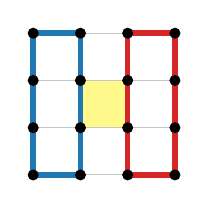
\begin{tikzpicture}[scale=0.6]
\fill[hicell] (1,1) rectangle (2,2);
\draw[gedge] (0,0) -- (1,0);
\draw[gedge] (0,0) -- (0,1);
\draw[gedge] (0,1) -- (1,1);
\draw[gedge] (0,1) -- (0,2);
\draw[gedge] (0,2) -- (1,2);
\draw[gedge] (0,2) -- (0,3);
\draw[gedge] (0,3) -- (1,3);
\draw[gedge] (1,0) -- (2,0);
\draw[gedge] (1,0) -- (1,1);
\draw[gedge] (1,1) -- (2,1);
\draw[gedge] (1,1) -- (1,2);
\draw[gedge] (1,2) -- (2,2);
\draw[gedge] (1,2) -- (1,3);
\draw[gedge] (1,3) -- (2,3);
\draw[gedge] (2,0) -- (3,0);
\draw[gedge] (2,0) -- (2,1);
\draw[gedge] (2,1) -- (3,1);
\draw[gedge] (2,1) -- (2,2);
\draw[gedge] (2,2) -- (3,2);
\draw[gedge] (2,2) -- (2,3);
\draw[gedge] (2,3) -- (3,3);
\draw[gedge] (3,0) -- (3,1);
\draw[gedge] (3,1) -- (3,2);
\draw[gedge] (3,2) -- (3,3);
\draw[pc1] (0,0) -- (1,0);
\draw[pc1] (0,3) -- (1,3);
\draw[pc1] (0,0) -- (0,1);
\draw[pc1] (0,1) -- (0,2);
\draw[pc1] (0,2) -- (0,3);
\draw[pc1] (1,0) -- (1,1);
\draw[pc1] (1,1) -- (1,2);
\draw[pc1] (1,2) -- (1,3);
\draw[pc2] (2,0) -- (3,0);
\draw[pc2] (2,3) -- (3,3);
\draw[pc2] (2,0) -- (2,1);
\draw[pc2] (2,1) -- (2,2);
\draw[pc2] (2,2) -- (2,3);
\draw[pc2] (3,0) -- (3,1);
\draw[pc2] (3,1) -- (3,2);
\draw[pc2] (3,2) -- (3,3);
\node[pt] at (0,0) {};
\node[pt] at (0,1) {};
\node[pt] at (0,2) {};
\node[pt] at (0,3) {};
\node[pt] at (1,0) {};
\node[pt] at (1,1) {};
\node[pt] at (1,2) {};
\node[pt] at (1,3) {};
\node[pt] at (2,0) {};
\node[pt] at (2,1) {};
\node[pt] at (2,2) {};
\node[pt] at (2,3) {};
\node[pt] at (3,0) {};
\node[pt] at (3,1) {};
\node[pt] at (3,2) {};
\node[pt] at (3,3) {};
\end{tikzpicture} & 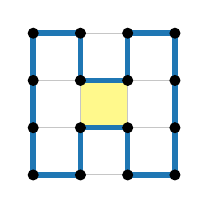
\begin{tikzpicture}[scale=0.6]
\fill[hicell] (1,1) rectangle (2,2);
\draw[gedge] (0,0) -- (1,0);
\draw[gedge] (0,0) -- (0,1);
\draw[gedge] (0,1) -- (1,1);
\draw[gedge] (0,1) -- (0,2);
\draw[gedge] (0,2) -- (1,2);
\draw[gedge] (0,2) -- (0,3);
\draw[gedge] (0,3) -- (1,3);
\draw[gedge] (1,0) -- (2,0);
\draw[gedge] (1,0) -- (1,1);
\draw[gedge] (1,1) -- (2,1);
\draw[gedge] (1,1) -- (1,2);
\draw[gedge] (1,2) -- (2,2);
\draw[gedge] (1,2) -- (1,3);
\draw[gedge] (1,3) -- (2,3);
\draw[gedge] (2,0) -- (3,0);
\draw[gedge] (2,0) -- (2,1);
\draw[gedge] (2,1) -- (3,1);
\draw[gedge] (2,1) -- (2,2);
\draw[gedge] (2,2) -- (3,2);
\draw[gedge] (2,2) -- (2,3);
\draw[gedge] (2,3) -- (3,3);
\draw[gedge] (3,0) -- (3,1);
\draw[gedge] (3,1) -- (3,2);
\draw[gedge] (3,2) -- (3,3);
\draw[pc1] (0,0) -- (1,0);
\draw[pc1] (0,3) -- (1,3);
\draw[pc1] (1,1) -- (2,1);
\draw[pc1] (1,2) -- (2,2);
\draw[pc1] (2,0) -- (3,0);
\draw[pc1] (2,3) -- (3,3);
\draw[pc1] (0,0) -- (0,1);
\draw[pc1] (0,1) -- (0,2);
\draw[pc1] (0,2) -- (0,3);
\draw[pc1] (1,0) -- (1,1);
\draw[pc1] (1,2) -- (1,3);
\draw[pc1] (2,0) -- (2,1);
\draw[pc1] (2,2) -- (2,3);
\draw[pc1] (3,0) -- (3,1);
\draw[pc1] (3,1) -- (3,2);
\draw[pc1] (3,2) -- (3,3);
\node[pt] at (0,0) {};
\node[pt] at (0,1) {};
\node[pt] at (0,2) {};
\node[pt] at (0,3) {};
\node[pt] at (1,0) {};
\node[pt] at (1,1) {};
\node[pt] at (1,2) {};
\node[pt] at (1,3) {};
\node[pt] at (2,0) {};
\node[pt] at (2,1) {};
\node[pt] at (2,2) {};
\node[pt] at (2,3) {};
\node[pt] at (3,0) {};
\node[pt] at (3,1) {};
\node[pt] at (3,2) {};
\node[pt] at (3,3) {};
\end{tikzpicture} & 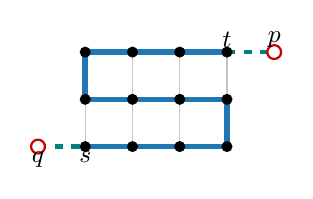
\begin{tikzpicture}[scale=0.6]
\draw[gedge] (0,0) -- (1,0);
\draw[gedge] (0,0) -- (0,1);
\draw[gedge] (0,1) -- (1,1);
\draw[gedge] (0,1) -- (0,2);
\draw[gedge] (0,2) -- (1,2);
\draw[gedge] (1,0) -- (2,0);
\draw[gedge] (1,0) -- (1,1);
\draw[gedge] (1,1) -- (2,1);
\draw[gedge] (1,1) -- (1,2);
\draw[gedge] (1,2) -- (2,2);
\draw[gedge] (2,0) -- (3,0);
\draw[gedge] (2,0) -- (2,1);
\draw[gedge] (2,1) -- (3,1);
\draw[gedge] (2,1) -- (2,2);
\draw[gedge] (2,2) -- (3,2);
\draw[gedge] (3,0) -- (3,1);
\draw[gedge] (3,1) -- (3,2);
\draw[pc1] (0,0) -- (1,0);
\draw[pc1] (1,0) -- (2,0);
\draw[pc1] (2,0) -- (3,0);
\draw[pc1] (3,0) -- (3,1);
\draw[pc1] (2,1) -- (3,1);
\draw[pc1] (1,1) -- (2,1);
\draw[pc1] (0,1) -- (1,1);
\draw[pc1] (0,1) -- (0,2);
\draw[pc1] (0,2) -- (1,2);
\draw[pc1] (1,2) -- (2,2);
\draw[pc1] (2,2) -- (3,2);
\draw[ph] (3,2) -- (4,2);
\draw[ph] (-1,0) -- (0,0);
\node[pt] at (0,0) {};
\node[pt] at (0,1) {};
\node[pt] at (0,2) {};
\node[pt] at (1,0) {};
\node[pt] at (1,1) {};
\node[pt] at (1,2) {};
\node[pt] at (2,0) {};
\node[pt] at (2,1) {};
\node[pt] at (2,2) {};
\node[pt] at (3,0) {};
\node[pt] at (3,1) {};
\node[pt] at (3,2) {};
\node[miss] at (4,2) {};
\node[miss] at (-1,0) {};
\node[lab,below] at (0,0) {$s$};
\node[lab,above] at (3,2) {$t$};
\node[lab,above] at (4,2) {$p$};
\node[lab,below] at (-1,0) {$q$};
\end{tikzpicture} & 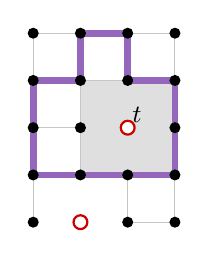
\begin{tikzpicture}[scale=0.6]
\fill[holecell] (1,1) rectangle (2,2);
\fill[holecell] (2,1) rectangle (3,2);
\fill[holecell] (1,2) rectangle (2,3);
\fill[holecell] (2,2) rectangle (3,3);
\draw[gedge] (0,0) -- (0,1);
\draw[gedge] (0,1) -- (1,1);
\draw[gedge] (0,1) -- (0,2);
\draw[gedge] (0,2) -- (1,2);
\draw[gedge] (0,2) -- (0,3);
\draw[gedge] (0,3) -- (1,3);
\draw[gedge] (0,3) -- (0,4);
\draw[gedge] (0,4) -- (1,4);
\draw[gedge] (1,1) -- (2,1);
\draw[gedge] (1,1) -- (1,2);
\draw[gedge] (1,2) -- (1,3);
\draw[gedge] (1,3) -- (2,3);
\draw[gedge] (1,3) -- (1,4);
\draw[gedge] (1,4) -- (2,4);
\draw[gedge] (2,0) -- (3,0);
\draw[gedge] (2,0) -- (2,1);
\draw[gedge] (2,1) -- (3,1);
\draw[gedge] (2,3) -- (3,3);
\draw[gedge] (2,3) -- (2,4);
\draw[gedge] (2,4) -- (3,4);
\draw[gedge] (3,0) -- (3,1);
\draw[gedge] (3,1) -- (3,2);
\draw[gedge] (3,2) -- (3,3);
\draw[gedge] (3,3) -- (3,4);
\draw[xedge] (0,1) -- (1,1);
\draw[xedge] (0,3) -- (1,3);
\draw[xedge] (1,1) -- (2,1);
\draw[xedge] (1,4) -- (2,4);
\draw[xedge] (2,1) -- (3,1);
\draw[xedge] (2,3) -- (3,3);
\draw[xedge] (0,1) -- (0,2);
\draw[xedge] (0,2) -- (0,3);
\draw[xedge] (1,3) -- (1,4);
\draw[xedge] (2,3) -- (2,4);
\draw[xedge] (3,1) -- (3,2);
\draw[xedge] (3,2) -- (3,3);
\node[pt] at (0,0) {};
\node[pt] at (0,1) {};
\node[pt] at (0,2) {};
\node[pt] at (0,3) {};
\node[pt] at (0,4) {};
\node[pt] at (1,1) {};
\node[pt] at (1,2) {};
\node[pt] at (1,3) {};
\node[pt] at (1,4) {};
\node[pt] at (2,0) {};
\node[pt] at (2,1) {};
\node[pt] at (2,3) {};
\node[pt] at (2,4) {};
\node[pt] at (3,0) {};
\node[pt] at (3,1) {};
\node[pt] at (3,2) {};
\node[pt] at (3,3) {};
\node[pt] at (3,4) {};
\node[miss] at (1,0) {};
\node[miss] at (2,2) {};
\node[lab,above right] at (2,2) {$t$};
\end{tikzpicture} \\
\small (a) two pieces & \small (b) one flip, one piece & \small (c) phantoms & \small (d) a loop around a hole
\end{tabular}

\caption{The ideas of the algorithm in four pictures.
(a) A $2$-factor of the $4\times4$ block with two pieces (blue, red).
The yellow cell has its left and right sides in the factor and its top and bottom sides out, and its
corners lie in two pieces.
(b) Flipping it (toggling its four sides) joins the two pieces into one cycle.
Sheffield's algorithm repeats such flips, ordered by a height function.
(c) A path from $s$ to $t$ with a phantom edge at each endpoint (dashed) to a missing point $p$ or
$q$ (red circles).
Now $s$ and $t$ have degree $2$, as in a cycle.
(d) An inner endpoint $t$ deleted, leaving a hole (grey cells).
Two path factors of $V\setminus\{t\}$ differ by the purple cycle, which goes around the hole.
No flip changes how many such cycles go around the hole, so the two factors lie in different
classes
(\cref{sec:classes}, \cref{fig:classes}).}
\label{fig:overview}
\end{figure}

Our algorithm reduces the path problem to situations where this machinery still works.
Every component below exists for one of two reasons.
Either it restores a hypothesis of Sheffield's argument that a path endpoint breaks, or it pays for
that repair with a bounded amount of branching.
A reader who keeps the cycle algorithm in mind can read each component as an answer to the
question ``what did the endpoint break, and how is it put back''.

\paragraph{Obstacle 1, endpoints have degree one.}
A Hamiltonian path has degree $1$ at $s$ and $t$.
Sheffield's local rules and his height function both use degree $2$ at every point.
The repair is a \emph{phantom} (\cref{sec:phantom}).
If an endpoint has a missing lattice neighbour $p$, the edge from the endpoint to $p$ is added.
The endpoint then has degree $2$, and the degree-one defect sits at $p$, outside $V$, where no cell
is ever flipped (\cref{fig:overview}c).
With phantoms at both endpoints, Sheffield's phase and certificate work again, provided the two
endpoints are at king distance at least $2$ and their phantoms do not point away from each other
across a gap of $2$ (the conditions \emph{Far} and \emph{not opposed}).
Most of \cref{sec:phantom} is the case analysis that proves this, and the reader can take
\cref{thm:twoph} as its summary.

\paragraph{Getting the endpoints into position.}
An endpoint may have no usable phantom, because it has no missing neighbour, or because the
endpoints are too close or opposed.
Then the algorithm deletes the endpoint and branches over its neighbour $w$ on the path.
$V$ has a Hamiltonian $s$--$t$ path exactly when $V\setminus\{t\}$ has one from $s$ to some neighbour
$w$ of $t$ (\cref{lem:del}), and the deleted $t$ becomes the phantom of $w$.
Repeating this is a \emph{deletion walk} (\cref{sec:walk,sec:one}).
Each end of the branching is a \emph{leaf}, a smaller set with a phantom at each endpoint, and the
algorithm runs a \emph{final test} there, Sheffield's loop with the class search of
\cref{sec:classes} when there are holes.
The walk is bookkeeping for correctness.
It makes at most $208$ final tests in every case, a constant, and when $s$ and $t$ are far apart the
walks stop right after the first deletions (\cref{sec:bulk}).

\paragraph{Obstacle 2, an inner endpoint leaves a hole.}
An endpoint whose eight king neighbours all lie in $V$ is \emph{inner}.
Deleting it leaves a one-point hole.
The deleted endpoint becomes the phantom of its neighbour on the path, so the degree-one defect
sits at the hole's centre.
Around this point the arcs do not balance, which we call a \emph{vortex}, and no height function
exists (\cref{sec:vortex}).
Two things are lost, and each is put back separately.
\begin{itemize}
\item \emph{The order of the flips.}
  The height is replaced by a \emph{slit height} that jumps across one ray from the vortex, plus a
  \emph{quadrant label}.
  Their combination still rises along every climb, which is the only property the certificate
  uses (\cref{thm:vortex}).
\item \emph{Reachability by flips.}
  Fix one factor $F$ of the leaf as a reference.
  Any other factor $G$ differs from $F$ by a set of alternating cycles, cycles whose edges lie
  alternately in $F$ and in $G$.
  Count the alternating cycles that go around the hole, with a sign for their direction.
  This number is the \emph{class} of $G$ (\cref{sec:classes}, with an informal picture at its
  start).
  A flip of $G$ changes the difference by the four sides of one cell.
  The four cells around the hole are not cells of the graph, so no flip changes how many cycles go
  around the hole, and the class never changes under flips (\cref{fig:overview}d).
  Factors in different classes cannot be reached from each other by flips, so one run of Sheffield's
  loop no longer decides the question.
  The algorithm therefore enumerates the classes, at most $2|V|+1$ per hole, builds the least factor
  of each class by a relaxation (\lean{classSearch}), and runs the loop in each class.
  Within one class Sheffield's argument works as before.
  \Cref{fig:classes} shows a leaf with two nonempty classes.
\end{itemize}
The class enumeration is the main source of the polynomial degree.
Two inner endpoints give two holes and at most $(2|V|+1)^2$ class pairs (\cref{sec:two}).

\paragraph{The loop.}
For each leaf of the deletion branching and each nonempty class, the algorithm runs Sheffield's
loop on two-phantom factors (\cref{sec:sheffield}).
Each round is a phase and a reduction.
A phase joins pieces by flipping a merging cell, and when none exists it builds \emph{bridges},
flips that split a piece to expose a merging cell.
The reduction then undoes or lowers the bridges, and the round ends with one piece fewer.
If a phase is stuck, the certificate proves that no factor of the class has fewer pieces than the
phase started with, and the
class is rejected.
The answer is yes exactly when some leaf and some class reach a single piece.
The count behind a stuck phase uses chained rows (\cref{sec:repair}).

\paragraph{What is essential and what is bookkeeping.}
\Cref{tab:components} lists the components.
The essential ideas are the phantom, the vortex potential, and the classes.
The rest makes them applicable everywhere, at a constant or polynomial price.

\begin{table}[t]
\centering
\small
\begin{tabular}{@{}>{\raggedright\arraybackslash}p{2.6cm}>{\raggedright\arraybackslash}p{4.4cm}>{\raggedright\arraybackslash}p{2.6cm}>{\raggedright\arraybackslash}p{1.9cm}>{\raggedright\arraybackslash}p{2.2cm}@{}}
\toprule
component & why it is there & cost & kind & where \\
\midrule
loop (phase, reduction, certificate) & Sheffield's cycle algorithm, joins pieces or proves none can be joined & $O(N^3)$ per round, $\le N$ rounds & core & \cref{sec:sheffield}, \cref{alg:twoPhantomLoop,alg:runPhase} \\
chained rows & complete the count for a stuck phase & none at run time & proof & \cref{sec:repair} \\
phantoms, Far, not opposed & give endpoints degree $2$ so the loop applies & constant & core & \cref{sec:phantom} \\
deletion walk & bring endpoints into the Far, not opposed position & $\le 16\cdot13$ final tests & bookkeeping & \cref{sec:walk,sec:one}, \cref{alg:boundaryEndpointsWalk,alg:holeCaseWalk} \\
slit height, quadrant label & replace the height at a vortex & none at run time & core (proof) & \cref{sec:vortex} \\
classes, class search & flips do not connect factors around a hole & $(2N)^k$ classes, $O(N^4)$ each & core & \cref{sec:classes}, \cref{alg:classSearch} \\
two vortices & both endpoints inner & as above, $k=2$ & core (proof) & \cref{sec:two} \\
\bottomrule
\end{tabular}
\caption{The components of the algorithm.
$N=|V|+3$, and $k$ is the number of inner endpoints.
``Core'' components carry the argument, ``bookkeeping'' components make it apply to every position
of the endpoints, and ``proof'' marks components that change the correctness proof but not the
computation.}
\label{tab:components}
\end{table}

\paragraph{Names.}
The procedures have the same names in the text, in the pseudocode of \cref{sec:time} and in Lean,
written \lean{decideHamPath} in Lean and \textsc{DecideHamPath} in the pseudocode.
\Cref{tab:names} lists them.
Lemma names extend the procedure names, for example \lean{decideHamPath\_main} and
\lean{boundaryEndpointsWalk\_correct}.

\begin{table}[t]
\centering
\small
\begin{tabular}{@{}>{\raggedright\arraybackslash}p{5.6cm}>{\raggedright\arraybackslash}p{6.6cm}>{\raggedright\arraybackslash}p{3.3cm}@{}}
\toprule
procedure & what it does & pseudocode \\
\midrule
\lean{decideHamPath} & dispatch on which endpoints are inner & \cref{alg:decideHamPath} \\
\lean{boundaryEndpoints}, \lean{boundaryEndpointsWalk} & no endpoint inner & \cref{alg:boundaryEndpoints,alg:boundaryEndpointsWalk} \\
\lean{holeCase}, \lean{holeCaseWalk} & delete $t$ and $s$, then walk & \cref{alg:holeCase,alg:holeCaseWalk} \\
\lean{oneHoleCase}, \lean{twoHoleCase} & one or two inner endpoints & \cref{alg:oneHoleCase} \\
\lean{oneHoleFinalTest}, \lean{twoHoleFinalTest} & the test at a leaf, class by class & \cref{alg:oneHoleFinalTest} \\
\lean{classSearch}, \lean{classSearchOne} & the least factor of a class, for several holes or one & \cref{alg:classSearch} \\
\lean{twoPhantomTest}, \lean{twoPhantomLoop} & Sheffield's loop with two phantoms & \cref{alg:twoPhantomLoop} \\
\lean{runPhase} & one phase & \cref{alg:runPhase} \\
\lean{reducePieces} & flip, then undo or lower the bridges & \cref{alg:reducePieces} \\
\lean{findFactor} & some factor with the given degrees & \cref{alg:findFactor} \\
\bottomrule
\end{tabular}
\caption{The procedures of the algorithm.
The same names are used in the text, in the pseudocode (in small capitals) and in Lean.}
\label{tab:names}
\end{table}

\paragraph{How to read the paper.}
A first reading can follow two concrete runs.
\Cref{sec:run} traces a small instance with one inner endpoint, where one leaf fails with a
certificate and the next succeeds.
\Cref{sec:bulk} traces an instance with two inner endpoints far apart, where the loop needs a
bridge.
The pseudocode in \cref{sec:time} gives the whole algorithm in one place.
After that, \cref{sec:sheffield} (the loop), \cref{sec:vortex} and \cref{sec:classes} (holes) carry
the main argument, and \cref{sec:phantom,sec:walk,sec:one} can be read for the endpoint details as
needed.

% =====================================================================
\section{Preliminaries}
\label{sec:prelim}

\subsection{Grid graphs, cells and solidity}

A \emph{point} is an element of $\Z^2$, written $(x,y)$.
\emph{Right} means increasing $x$ and \emph{up} means increasing $y$.
The \emph{king distance} of two points is $\dist(p,p')=\max(|x-x'|,|y-y'|)$.
The \emph{king neighbours} of $p$ are the eight points at king distance $1$.
The \emph{lattice neighbours} of $p$ are the four points at Euclidean distance $1$.

\begin{definition}[grid graph, edge, cell]
\label{def:grid}
Let $V\subset\Z^2$ be finite.
An \emph{edge} of $V$ is a unit segment whose two ends lie in $V$ (Lean \lean{IsEdge}).
The \emph{grid graph} on $V$ has these edges.
A \emph{square} is a unit square with lattice corners.
It is named by its lower-left corner $c$, so the square $c=(x,y)$ has corners $(x,y)$,
$(x+1,y)$, $(x,y+1)$, $(x+1,y+1)$.
A square is a \emph{cell} of $V$ when all four corners lie in $V$ (Lean \lean{IsCell}).
The four edges of a square are its \emph{sides}, named bottom, top, left and right.
\end{definition}

\begin{definition}[solid]
\label{def:solid}
A point $a\notin V$ is a \emph{missing point}.
$V$ is \emph{solid} when every missing point is joined, by a sequence of king moves through
missing points, to a point strictly left of all of $V$ (Lean \lean{Solid}, \lean{Algorithm.lean}).
\end{definition}

\Cref{fig:solid} shows a solid set and a set that is not solid.
A bounded face of area greater than one contains a missing point that cannot escape in this way.

\begin{figure}[t]
\centering
% SPDX-License-Identifier: CC0-1.0
% Generated by gen.py; do not edit by hand.
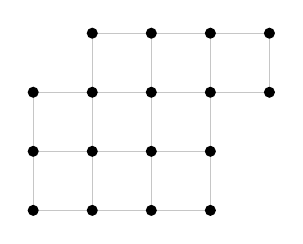
\begin{tikzpicture}[scale=0.75]
\draw[gedge] (0,0) -- (1,0);
\draw[gedge] (0,0) -- (0,1);
\draw[gedge] (0,1) -- (1,1);
\draw[gedge] (0,1) -- (0,2);
\draw[gedge] (0,2) -- (1,2);
\draw[gedge] (1,0) -- (2,0);
\draw[gedge] (1,0) -- (1,1);
\draw[gedge] (1,1) -- (2,1);
\draw[gedge] (1,1) -- (1,2);
\draw[gedge] (1,2) -- (2,2);
\draw[gedge] (1,2) -- (1,3);
\draw[gedge] (1,3) -- (2,3);
\draw[gedge] (2,0) -- (3,0);
\draw[gedge] (2,0) -- (2,1);
\draw[gedge] (2,1) -- (3,1);
\draw[gedge] (2,1) -- (2,2);
\draw[gedge] (2,2) -- (3,2);
\draw[gedge] (2,2) -- (2,3);
\draw[gedge] (2,3) -- (3,3);
\draw[gedge] (3,0) -- (3,1);
\draw[gedge] (3,1) -- (3,2);
\draw[gedge] (3,2) -- (4,2);
\draw[gedge] (3,2) -- (3,3);
\draw[gedge] (3,3) -- (4,3);
\draw[gedge] (4,2) -- (4,3);
\node[pt] at (0,0) {};
\node[pt] at (0,1) {};
\node[pt] at (0,2) {};
\node[pt] at (1,0) {};
\node[pt] at (1,1) {};
\node[pt] at (1,2) {};
\node[pt] at (1,3) {};
\node[pt] at (2,0) {};
\node[pt] at (2,1) {};
\node[pt] at (2,2) {};
\node[pt] at (2,3) {};
\node[pt] at (3,0) {};
\node[pt] at (3,1) {};
\node[pt] at (3,2) {};
\node[pt] at (3,3) {};
\node[pt] at (4,2) {};
\node[pt] at (4,3) {};
\end{tikzpicture}\qquad
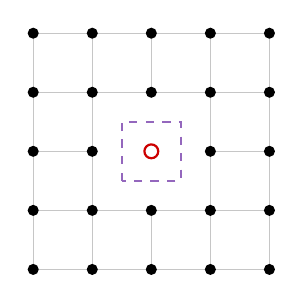
\begin{tikzpicture}[scale=0.75]
\draw[gedge] (0,0) -- (1,0);
\draw[gedge] (0,0) -- (0,1);
\draw[gedge] (0,1) -- (1,1);
\draw[gedge] (0,1) -- (0,2);
\draw[gedge] (0,2) -- (1,2);
\draw[gedge] (0,2) -- (0,3);
\draw[gedge] (0,3) -- (1,3);
\draw[gedge] (0,3) -- (0,4);
\draw[gedge] (0,4) -- (1,4);
\draw[gedge] (1,0) -- (2,0);
\draw[gedge] (1,0) -- (1,1);
\draw[gedge] (1,1) -- (2,1);
\draw[gedge] (1,1) -- (1,2);
\draw[gedge] (1,2) -- (1,3);
\draw[gedge] (1,3) -- (2,3);
\draw[gedge] (1,3) -- (1,4);
\draw[gedge] (1,4) -- (2,4);
\draw[gedge] (2,0) -- (3,0);
\draw[gedge] (2,0) -- (2,1);
\draw[gedge] (2,1) -- (3,1);
\draw[gedge] (2,3) -- (3,3);
\draw[gedge] (2,3) -- (2,4);
\draw[gedge] (2,4) -- (3,4);
\draw[gedge] (3,0) -- (4,0);
\draw[gedge] (3,0) -- (3,1);
\draw[gedge] (3,1) -- (4,1);
\draw[gedge] (3,1) -- (3,2);
\draw[gedge] (3,2) -- (4,2);
\draw[gedge] (3,2) -- (3,3);
\draw[gedge] (3,3) -- (4,3);
\draw[gedge] (3,3) -- (3,4);
\draw[gedge] (3,4) -- (4,4);
\draw[gedge] (4,0) -- (4,1);
\draw[gedge] (4,1) -- (4,2);
\draw[gedge] (4,2) -- (4,3);
\draw[gedge] (4,3) -- (4,4);
\node[pt] at (0,0) {};
\node[pt] at (0,1) {};
\node[pt] at (0,2) {};
\node[pt] at (0,3) {};
\node[pt] at (0,4) {};
\node[pt] at (1,0) {};
\node[pt] at (1,1) {};
\node[pt] at (1,2) {};
\node[pt] at (1,3) {};
\node[pt] at (1,4) {};
\node[pt] at (2,0) {};
\node[pt] at (2,1) {};
\node[pt] at (2,3) {};
\node[pt] at (2,4) {};
\node[pt] at (3,0) {};
\node[pt] at (3,1) {};
\node[pt] at (3,2) {};
\node[pt] at (3,3) {};
\node[pt] at (3,4) {};
\node[pt] at (4,0) {};
\node[pt] at (4,1) {};
\node[pt] at (4,2) {};
\node[pt] at (4,3) {};
\node[pt] at (4,4) {};
\node[miss] at (2,2) {};
\draw[king] (1.5,1.5) rectangle (2.5,2.5);
\end{tikzpicture}

\caption{Left: a solid grid graph.
Right: not solid.
The red point is missing.
All eight of its king neighbours (inside the purple dashed box) are in $V$, so it cannot reach the
outside by king moves through missing points.}
\label{fig:solid}
\end{figure}

\begin{definition}[inner point]
A point $p$ is \emph{inner} in $V$ when the four squares with corner $p$ are cells of $V$
(Lean \lean{Inner}, decided by \lean{isInner}).
An inner point lies in $V$, and a point of $V$ is inner exactly when all eight of its king
neighbours lie in $V$.
A point of $V$ that is not inner has a missing king neighbour (\lean{miss\_of\_not\_inner}).
\end{definition}

\subsection{Factors and pieces}

\begin{definition}[factor, path factor, piece]
Let $d\colon\Z^2\to\mathbb N$.
A \emph{factor} of $V$ with degrees $d$ is a set $H$ of edges of $V$ in which every $p\in V$ has
degree $d(p)$ (Lean \lean{IsFactor}).
For $s\neq t$ let $d_{st}$ be $1$ at $s$ and $t$ and $2$ elsewhere (Lean \lean{dST}).
A factor with degrees $d_{st}$ is a \emph{path factor}.
The connected components of $H$ on $V$ are its \emph{pieces}, and $\ncomp(V,H)$ is their number
(Lean \lean{ncomp}).
\end{definition}

A path factor consists of one path from $s$ to $t$ and some cycles.
It is a Hamiltonian $s$--$t$ path exactly when it has one piece (\cref{fig:factor}, left).
An edge of $H$ is called \emph{dark}.
An edge of $V$ not in $H$ is called \emph{light}.

\paragraph{Finding a factor.}
Every run starts from some factor with prescribed degrees $d\le2$.
The grid graph is bipartite, so such a factor is an integral maximum flow in the standard
source--black--white--sink network, with capacity $d$ at the points and $1$ on the edges.
\lean{findFactor} (\lean{Algorithm.lean}, \cref{alg:findFactor}) runs the Ford--Fulkerson method on
this network, with at most $|V|+1$ augmentations and every choice fixed.
It returns a factor when one exists (\lean{findFactor\_some}), and returns none only when no factor
exists (\lean{findFactor\_none}), at cost $O((|V|+1)^3)$ (\lean{DFC.findFactorCost\_le}).
The factor can have several pieces, as in \cref{fig:example}c and \cref{fig:classsearch}a.
\Cref{app:flow} gives the network, the colour conditions that degree $1$ at $s$ and $t$ imposes,
and two examples.

\begin{figure}[t]
\centering
% SPDX-License-Identifier: CC0-1.0
% Generated by gen.py; do not edit by hand.
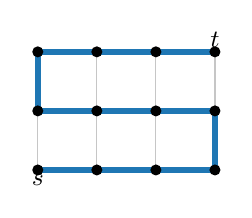
\begin{tikzpicture}[scale=0.75]
\draw[gedge] (0,0) -- (1,0);
\draw[gedge] (0,0) -- (0,1);
\draw[gedge] (0,1) -- (1,1);
\draw[gedge] (0,1) -- (0,2);
\draw[gedge] (0,2) -- (1,2);
\draw[gedge] (1,0) -- (2,0);
\draw[gedge] (1,0) -- (1,1);
\draw[gedge] (1,1) -- (2,1);
\draw[gedge] (1,1) -- (1,2);
\draw[gedge] (1,2) -- (2,2);
\draw[gedge] (2,0) -- (3,0);
\draw[gedge] (2,0) -- (2,1);
\draw[gedge] (2,1) -- (3,1);
\draw[gedge] (2,1) -- (2,2);
\draw[gedge] (2,2) -- (3,2);
\draw[gedge] (3,0) -- (3,1);
\draw[gedge] (3,1) -- (3,2);
\draw[pc1] (0,0) -- (1,0);
\draw[pc1] (1,0) -- (2,0);
\draw[pc1] (2,0) -- (3,0);
\draw[pc1] (3,0) -- (3,1);
\draw[pc1] (2,1) -- (3,1);
\draw[pc1] (1,1) -- (2,1);
\draw[pc1] (0,1) -- (1,1);
\draw[pc1] (0,1) -- (0,2);
\draw[pc1] (0,2) -- (1,2);
\draw[pc1] (1,2) -- (2,2);
\draw[pc1] (2,2) -- (3,2);
\node[pt] at (0,0) {};
\node[pt] at (0,1) {};
\node[pt] at (0,2) {};
\node[pt] at (1,0) {};
\node[pt] at (1,1) {};
\node[pt] at (1,2) {};
\node[pt] at (2,0) {};
\node[pt] at (2,1) {};
\node[pt] at (2,2) {};
\node[pt] at (3,0) {};
\node[pt] at (3,1) {};
\node[pt] at (3,2) {};
\node[lab,below] at (0,0) {$s$};
\node[lab,above] at (3,2) {$t$};
\end{tikzpicture}\qquad
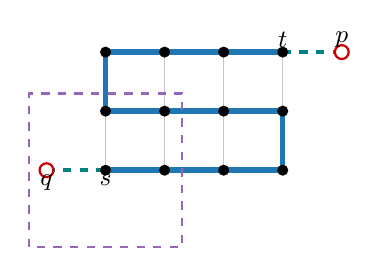
\begin{tikzpicture}[scale=0.75]
\draw[gedge] (0,0) -- (1,0);
\draw[gedge] (0,0) -- (0,1);
\draw[gedge] (0,1) -- (1,1);
\draw[gedge] (0,1) -- (0,2);
\draw[gedge] (0,2) -- (1,2);
\draw[gedge] (1,0) -- (2,0);
\draw[gedge] (1,0) -- (1,1);
\draw[gedge] (1,1) -- (2,1);
\draw[gedge] (1,1) -- (1,2);
\draw[gedge] (1,2) -- (2,2);
\draw[gedge] (2,0) -- (3,0);
\draw[gedge] (2,0) -- (2,1);
\draw[gedge] (2,1) -- (3,1);
\draw[gedge] (2,1) -- (2,2);
\draw[gedge] (2,2) -- (3,2);
\draw[gedge] (3,0) -- (3,1);
\draw[gedge] (3,1) -- (3,2);
\draw[pc1] (0,0) -- (1,0);
\draw[pc1] (1,0) -- (2,0);
\draw[pc1] (2,0) -- (3,0);
\draw[pc1] (3,0) -- (3,1);
\draw[pc1] (2,1) -- (3,1);
\draw[pc1] (1,1) -- (2,1);
\draw[pc1] (0,1) -- (1,1);
\draw[pc1] (0,1) -- (0,2);
\draw[pc1] (0,2) -- (1,2);
\draw[pc1] (1,2) -- (2,2);
\draw[pc1] (2,2) -- (3,2);
\draw[ph] (3,2) -- (4,2);
\draw[ph] (-1,0) -- (0,0);
\node[pt] at (0,0) {};
\node[pt] at (0,1) {};
\node[pt] at (0,2) {};
\node[pt] at (1,0) {};
\node[pt] at (1,1) {};
\node[pt] at (1,2) {};
\node[pt] at (2,0) {};
\node[pt] at (2,1) {};
\node[pt] at (2,2) {};
\node[pt] at (3,0) {};
\node[pt] at (3,1) {};
\node[pt] at (3,2) {};
\node[miss] at (4,2) {};
\node[miss] at (-1,0) {};
\node[lab,below] at (0,0) {$s$};
\node[lab,above] at (3,2) {$t$};
\node[lab,above] at (4,2) {$p$};
\node[lab,below] at (-1,0) {$q$};
\draw[king] (-1.3,-1.3) rectangle (1.3,1.3);
\end{tikzpicture}

\caption{Left: a path factor with one piece, a Hamiltonian path from $s$ to $t$.
Right: the same path with two phantom edges (dashed, \cref{sec:phantom}).
The missing points $p$ and $q$ are phantoms, and $t$ and $s$ now have degree $2$.
The purple box holds the points within king distance $1$ of $s$.
The point $t$ lies outside it, so $s$ and $t$ are Far (\cref{def:far}).
Their phantoms are not opposed, because $t$ and $s$ differ by $3$ in $x$.}
\label{fig:factor}
\end{figure}

\subsection{Arcs and heights}

The \emph{colour} of a square $c=(x,y)$ is the parity of $x+y$ (Lean \lean{par}).
Two squares that share a side have different colours.

\begin{definition}[arc]
\label{def:arc}
Let $H$ be a set of edges and let $c$ be a square with a side $e$.
The \emph{arc} of $H$ across $e$ points out of $c$ exactly in the following cases (Lean
\lean{outArc}, closed form \lean{outArc\_eq}).
\begin{itemize}
\item $e$ is horizontal, and either $c$ is odd and $e$ is dark, or $c$ is even and $e$ is light.
\item $e$ is vertical, and either $c$ is odd and $e$ is light, or $c$ is even and $e$ is dark.
\end{itemize}
Otherwise the arc points into $c$.
\end{definition}

Colour the points like a checkerboard, a point $(x,y)$ \emph{black} when $x+y$ is even and
\emph{white} otherwise (Lean \lean{Black}).
Every edge joins a black point to a white point.
The colour of the square on each side of an edge is fixed by which end of the edge is black, so
\cref{def:arc} can be restated without cell colours.
Walk along an edge from its black end to its white end.
If the edge is dark, its arc crosses it from right to left.
If the edge is light, its arc crosses it from left to right.
To see this, let $e$ run from $(x,y)$ one step right or up, and let $\beta$ be true when $x+y$ is
even, so that the square below or left of $e$ is odd exactly when $\beta$ holds.
For horizontal $e$, \cref{def:arc} applied to the square below says that the arc points up exactly
when $e$ is dark and $\beta$ holds or $e$ is light and $\beta$ fails.
The walk goes right from $(x,y)$ when $\beta$ holds, so up is on its left, and left from $(x+1,y)$
otherwise, so up is on its right.
For vertical $e$, \cref{def:arc} applied to the square left of $e$ says that the arc points right
exactly when $e$ is light and $\beta$ holds or $e$ is dark and $\beta$ fails.
The walk goes up from $(x,y)$ when $\beta$ holds, so right is on its right, and down from
$(x,y+1)$ otherwise, so right is on its left.
In all four cases a dark edge's arc crosses from right to left and a light edge's from left to
right.

The rule is antisymmetric.
Seen from the square on the other side of $e$ (of the other colour), the same arc points in.
So each side between two squares carries one arc, pointing from one square to the other.
Toggling the membership of $e$ reverses its arc.

\begin{definition}[height]
A \emph{height} of $H$ on the cells of $V$ is a function $\tau$ on cells with
$\tau(c')=\tau(c)+1$ whenever the arc across the side between cells $c$ and $c'$ points from $c$
to $c'$ (Lean \lean{HeightOn}).
\end{definition}

\Cref{fig:arcs} shows the arcs of a Hamiltonian cycle on a $4\times3$ block and its height.
Each arc is drawn as a short arrow across the side it belongs to.
The height rises by $1$ along every arrow.

\begin{figure}[t]
\centering
% SPDX-License-Identifier: CC0-1.0
% Generated by gen.py; do not edit by hand.
\begin{tabular}{c@{\qquad}c}
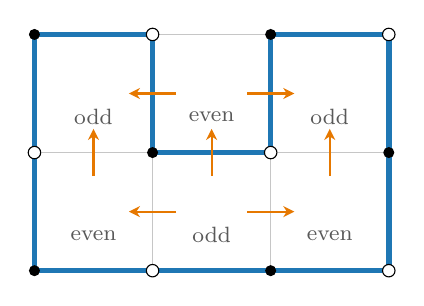
\begin{tikzpicture}[scale=1.5]
\draw[gedge] (0,0) -- (1,0);
\draw[gedge] (0,0) -- (0,1);
\draw[gedge] (0,1) -- (1,1);
\draw[gedge] (0,1) -- (0,2);
\draw[gedge] (0,2) -- (1,2);
\draw[gedge] (1,0) -- (2,0);
\draw[gedge] (1,0) -- (1,1);
\draw[gedge] (1,1) -- (2,1);
\draw[gedge] (1,1) -- (1,2);
\draw[gedge] (1,2) -- (2,2);
\draw[gedge] (2,0) -- (3,0);
\draw[gedge] (2,0) -- (2,1);
\draw[gedge] (2,1) -- (3,1);
\draw[gedge] (2,1) -- (2,2);
\draw[gedge] (2,2) -- (3,2);
\draw[gedge] (3,0) -- (3,1);
\draw[gedge] (3,1) -- (3,2);
\draw[pc1] (0,0) -- (1,0);
\draw[pc1] (0,2) -- (1,2);
\draw[pc1] (1,0) -- (2,0);
\draw[pc1] (1,1) -- (2,1);
\draw[pc1] (2,0) -- (3,0);
\draw[pc1] (2,2) -- (3,2);
\draw[pc1] (0,0) -- (0,1);
\draw[pc1] (0,1) -- (0,2);
\draw[pc1] (1,1) -- (1,2);
\draw[pc1] (2,1) -- (2,2);
\draw[pc1] (3,0) -- (3,1);
\draw[pc1] (3,1) -- (3,2);
\node[pt] at (0,0) {};
\node[wpt] at (0,1) {};
\node[pt] at (0,2) {};
\node[wpt] at (1,0) {};
\node[pt] at (1,1) {};
\node[wpt] at (1,2) {};
\node[pt] at (2,0) {};
\node[wpt] at (2,1) {};
\node[pt] at (2,2) {};
\node[wpt] at (3,0) {};
\node[pt] at (3,1) {};
\node[wpt] at (3,2) {};
\node[cellname] at (0+0.5,0+0.3) {even};
\node[cellname] at (0+0.5,1+0.3) {odd};
\node[cellname] at (1+0.5,0+0.3) {odd};
\node[cellname] at (1+0.5,1+0.3) {even};
\node[cellname] at (2+0.5,0+0.3) {even};
\node[cellname] at (2+0.5,1+0.3) {odd};
\draw[arcarrow] (0.50,0.80) -- (0.50,1.20);
\draw[arcarrow] (1.20,0.50) -- (0.80,0.50);
\draw[arcarrow] (1.20,1.50) -- (0.80,1.50);
\draw[arcarrow] (1.50,0.80) -- (1.50,1.20);
\draw[arcarrow] (1.80,0.50) -- (2.20,0.50);
\draw[arcarrow] (1.80,1.50) -- (2.20,1.50);
\draw[arcarrow] (2.50,0.80) -- (2.50,1.20);
\end{tikzpicture} & 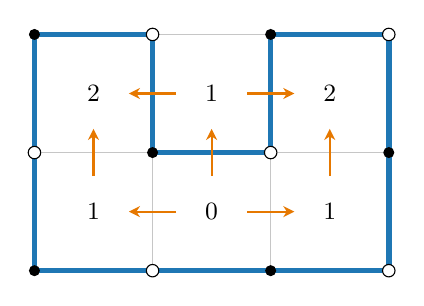
\begin{tikzpicture}[scale=1.5]
\draw[gedge] (0,0) -- (1,0);
\draw[gedge] (0,0) -- (0,1);
\draw[gedge] (0,1) -- (1,1);
\draw[gedge] (0,1) -- (0,2);
\draw[gedge] (0,2) -- (1,2);
\draw[gedge] (1,0) -- (2,0);
\draw[gedge] (1,0) -- (1,1);
\draw[gedge] (1,1) -- (2,1);
\draw[gedge] (1,1) -- (1,2);
\draw[gedge] (1,2) -- (2,2);
\draw[gedge] (2,0) -- (3,0);
\draw[gedge] (2,0) -- (2,1);
\draw[gedge] (2,1) -- (3,1);
\draw[gedge] (2,1) -- (2,2);
\draw[gedge] (2,2) -- (3,2);
\draw[gedge] (3,0) -- (3,1);
\draw[gedge] (3,1) -- (3,2);
\draw[pc1] (0,0) -- (1,0);
\draw[pc1] (0,2) -- (1,2);
\draw[pc1] (1,0) -- (2,0);
\draw[pc1] (1,1) -- (2,1);
\draw[pc1] (2,0) -- (3,0);
\draw[pc1] (2,2) -- (3,2);
\draw[pc1] (0,0) -- (0,1);
\draw[pc1] (0,1) -- (0,2);
\draw[pc1] (1,1) -- (1,2);
\draw[pc1] (2,1) -- (2,2);
\draw[pc1] (3,0) -- (3,1);
\draw[pc1] (3,1) -- (3,2);
\node[pt] at (0,0) {};
\node[wpt] at (0,1) {};
\node[pt] at (0,2) {};
\node[wpt] at (1,0) {};
\node[pt] at (1,1) {};
\node[wpt] at (1,2) {};
\node[pt] at (2,0) {};
\node[wpt] at (2,1) {};
\node[pt] at (2,2) {};
\node[wpt] at (3,0) {};
\node[pt] at (3,1) {};
\node[wpt] at (3,2) {};
\draw[arcarrow] (0.50,0.80) -- (0.50,1.20);
\draw[arcarrow] (1.20,0.50) -- (0.80,0.50);
\draw[arcarrow] (1.20,1.50) -- (0.80,1.50);
\draw[arcarrow] (1.50,0.80) -- (1.50,1.20);
\draw[arcarrow] (1.80,0.50) -- (2.20,0.50);
\draw[arcarrow] (1.80,1.50) -- (2.20,1.50);
\draw[arcarrow] (2.50,0.80) -- (2.50,1.20);
\node[taulab] at (0+0.5,0+0.5) {$1$};
\node[taulab] at (0+0.5,1+0.5) {$2$};
\node[taulab] at (1+0.5,0+0.5) {$0$};
\node[taulab] at (1+0.5,1+0.5) {$1$};
\node[taulab] at (2+0.5,0+0.5) {$1$};
\node[taulab] at (2+0.5,1+0.5) {$2$};
\end{tikzpicture} \\
\small (a) arcs & \small (b) a height $\tau$
\end{tabular}

\caption{(a) A Hamiltonian cycle (blue) on a $4\times3$ block, the colour of each cell, the checkerboard
colour of each point (black or white), and the arc across each side between two cells (orange
arrows).
Walking along an edge from its black end to its white end, the arc of a dark edge points left and
the arc of a light edge points right.
The side between the even cell $(0,0)$ and the odd cell $(1,0)$ is vertical and light, so by
\cref{def:arc} its arc points into $(0,0)$.
(b) The same arcs with a height $\tau$ written in each cell, normalised so the least value is $0$.
Every arrow goes from a cell to a cell whose height is larger by $1$.}
\label{fig:arcs}
\end{figure}

Around a point $v$, the four squares with corner $v$ are separated by the four edges at $v$.
Going once around $v$, the arcs add up to $\pm(4-2\deg_H v)$, with the sign fixed by the colour of
$v$.
To see this, go counterclockwise around a black $v$.
Facing outward along an edge at $v$, the walk crosses it from right to left.
By the rule above a dark edge's arc crosses the same way and a light edge's the other way, so the
four arcs add up to $\deg_H v-(4-\deg_H v)=2\deg_H v-4$.
For a white $v$, facing outward walks from white to black, so both signs reverse and the sum is
$4-2\deg_H v$.
So the arcs balance at a point of degree $2$.

\begin{lemma}[\lean{height\_exists}, \lean{Height.lean}]
\label{lem:height}
If $V$ is solid and every inner point has degree $2$ in $H$, then $H$ has a height on the cells
of $V$.
\end{lemma}

\begin{proof}
This is the argument of \cref{app:slit} without a vortex.
The four edges at an inner point are sides between two cells, so the arcs balance there.
At a point that is not inner the arcs need not balance, and the imbalance is moved along a path of
edges that are not sides between two cells to a point far left of $V$, which exists because $V$ is
solid.
These corrections change no arc between two cells.
Afterwards the weights balance at every point, so they are the jumps of a function $\tau$, which is
a height.
\end{proof}

\begin{definition}[relative height $D$]
\label{def:D}
Let $F$ and $H$ be edge sets.
Their \emph{symmetric difference} is $F\oplus H=(F\setminus H)\cup(H\setminus F)$, the set of
edges that lie in exactly one of $F$ and $H$.
Give each edge $e$ of $F\oplus H$ the weight $+2$ if the arc of $F$ across $e$ points from its
lower or left square to its upper or right square, and $-2$ otherwise.
$D(F,H)(c)$ is the sum of these weights over the vertical edges of $F\oplus H$ in the row of
$c$ at or left of the left side of $c$ (Lean \lean{D}, \lean{D.lean}).
\end{definition}

When $F$ and $H$ have the same degrees at every point, $D(F,H)$ changes by $\pm2$ across each side
in $F\oplus H$ and by $0$ across every other side.
Its sign across $e\in F\oplus H$ is $+$ in the direction of the arc of $F$.
When both factors have heights, $D(F,H)=\tau_F-\tau_H$ up to a constant.
$D$ needs no boundary values, and it is defined for path factors as well.
\Cref{fig:D} shows two factors that differ at one cell.

\begin{figure}[t]
\centering
% SPDX-License-Identifier: CC0-1.0
% Generated by gen.py; do not edit by hand.
\begin{tabular}{c@{\quad}c@{\quad}c}
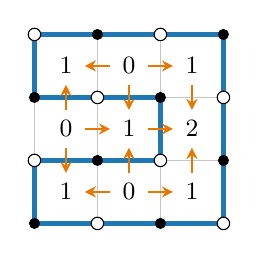
\begin{tikzpicture}[scale=0.8]
\draw[gedge] (0,0) -- (1,0);
\draw[gedge] (0,0) -- (0,1);
\draw[gedge] (0,1) -- (1,1);
\draw[gedge] (0,1) -- (0,2);
\draw[gedge] (0,2) -- (1,2);
\draw[gedge] (0,2) -- (0,3);
\draw[gedge] (0,3) -- (1,3);
\draw[gedge] (1,0) -- (2,0);
\draw[gedge] (1,0) -- (1,1);
\draw[gedge] (1,1) -- (2,1);
\draw[gedge] (1,1) -- (1,2);
\draw[gedge] (1,2) -- (2,2);
\draw[gedge] (1,2) -- (1,3);
\draw[gedge] (1,3) -- (2,3);
\draw[gedge] (2,0) -- (3,0);
\draw[gedge] (2,0) -- (2,1);
\draw[gedge] (2,1) -- (3,1);
\draw[gedge] (2,1) -- (2,2);
\draw[gedge] (2,2) -- (3,2);
\draw[gedge] (2,2) -- (2,3);
\draw[gedge] (2,3) -- (3,3);
\draw[gedge] (3,0) -- (3,1);
\draw[gedge] (3,1) -- (3,2);
\draw[gedge] (3,2) -- (3,3);
\draw[pc1] (0,0) -- (1,0);
\draw[pc1] (0,1) -- (1,1);
\draw[pc1] (0,2) -- (1,2);
\draw[pc1] (0,3) -- (1,3);
\draw[pc1] (1,0) -- (2,0);
\draw[pc1] (1,1) -- (2,1);
\draw[pc1] (1,2) -- (2,2);
\draw[pc1] (1,3) -- (2,3);
\draw[pc1] (2,0) -- (3,0);
\draw[pc1] (2,3) -- (3,3);
\draw[pc1] (0,0) -- (0,1);
\draw[pc1] (0,2) -- (0,3);
\draw[pc1] (2,1) -- (2,2);
\draw[pc1] (3,0) -- (3,1);
\draw[pc1] (3,1) -- (3,2);
\draw[pc1] (3,2) -- (3,3);
\node[pt] at (0,0) {};
\node[wpt] at (0,1) {};
\node[pt] at (0,2) {};
\node[wpt] at (0,3) {};
\node[wpt] at (1,0) {};
\node[pt] at (1,1) {};
\node[wpt] at (1,2) {};
\node[pt] at (1,3) {};
\node[pt] at (2,0) {};
\node[wpt] at (2,1) {};
\node[pt] at (2,2) {};
\node[wpt] at (2,3) {};
\node[wpt] at (3,0) {};
\node[pt] at (3,1) {};
\node[wpt] at (3,2) {};
\node[pt] at (3,3) {};
\draw[arcarrow] (0.50,1.20) -- (0.50,0.80);
\draw[arcarrow] (1.20,0.50) -- (0.80,0.50);
\draw[arcarrow] (0.50,1.80) -- (0.50,2.20);
\draw[arcarrow] (0.80,1.50) -- (1.20,1.50);
\draw[arcarrow] (1.20,2.50) -- (0.80,2.50);
\draw[arcarrow] (1.50,0.80) -- (1.50,1.20);
\draw[arcarrow] (1.80,0.50) -- (2.20,0.50);
\draw[arcarrow] (1.50,2.20) -- (1.50,1.80);
\draw[arcarrow] (1.80,1.50) -- (2.20,1.50);
\draw[arcarrow] (1.80,2.50) -- (2.20,2.50);
\draw[arcarrow] (2.50,0.80) -- (2.50,1.20);
\draw[arcarrow] (2.50,2.20) -- (2.50,1.80);
\node[taulab] at (0+0.5,0+0.5) {$1$};
\node[taulab] at (0+0.5,1+0.5) {$0$};
\node[taulab] at (0+0.5,2+0.5) {$1$};
\node[taulab] at (1+0.5,0+0.5) {$0$};
\node[taulab] at (1+0.5,1+0.5) {$1$};
\node[taulab] at (1+0.5,2+0.5) {$0$};
\node[taulab] at (2+0.5,0+0.5) {$1$};
\node[taulab] at (2+0.5,1+0.5) {$2$};
\node[taulab] at (2+0.5,2+0.5) {$1$};
\end{tikzpicture} & 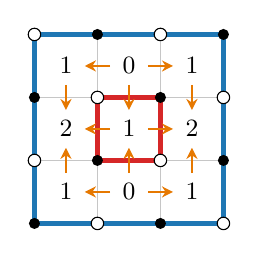
\begin{tikzpicture}[scale=0.8]
\draw[gedge] (0,0) -- (1,0);
\draw[gedge] (0,0) -- (0,1);
\draw[gedge] (0,1) -- (1,1);
\draw[gedge] (0,1) -- (0,2);
\draw[gedge] (0,2) -- (1,2);
\draw[gedge] (0,2) -- (0,3);
\draw[gedge] (0,3) -- (1,3);
\draw[gedge] (1,0) -- (2,0);
\draw[gedge] (1,0) -- (1,1);
\draw[gedge] (1,1) -- (2,1);
\draw[gedge] (1,1) -- (1,2);
\draw[gedge] (1,2) -- (2,2);
\draw[gedge] (1,2) -- (1,3);
\draw[gedge] (1,3) -- (2,3);
\draw[gedge] (2,0) -- (3,0);
\draw[gedge] (2,0) -- (2,1);
\draw[gedge] (2,1) -- (3,1);
\draw[gedge] (2,1) -- (2,2);
\draw[gedge] (2,2) -- (3,2);
\draw[gedge] (2,2) -- (2,3);
\draw[gedge] (2,3) -- (3,3);
\draw[gedge] (3,0) -- (3,1);
\draw[gedge] (3,1) -- (3,2);
\draw[gedge] (3,2) -- (3,3);
\draw[pc1] (0,0) -- (1,0);
\draw[pc1] (0,3) -- (1,3);
\draw[pc1] (1,0) -- (2,0);
\draw[pc1] (1,3) -- (2,3);
\draw[pc1] (2,0) -- (3,0);
\draw[pc1] (2,3) -- (3,3);
\draw[pc1] (0,0) -- (0,1);
\draw[pc1] (0,1) -- (0,2);
\draw[pc1] (0,2) -- (0,3);
\draw[pc1] (3,0) -- (3,1);
\draw[pc1] (3,1) -- (3,2);
\draw[pc1] (3,2) -- (3,3);
\draw[pc2] (1,1) -- (2,1);
\draw[pc2] (1,2) -- (2,2);
\draw[pc2] (1,1) -- (1,2);
\draw[pc2] (2,1) -- (2,2);
\node[pt] at (0,0) {};
\node[wpt] at (0,1) {};
\node[pt] at (0,2) {};
\node[wpt] at (0,3) {};
\node[wpt] at (1,0) {};
\node[pt] at (1,1) {};
\node[wpt] at (1,2) {};
\node[pt] at (1,3) {};
\node[pt] at (2,0) {};
\node[wpt] at (2,1) {};
\node[pt] at (2,2) {};
\node[wpt] at (2,3) {};
\node[wpt] at (3,0) {};
\node[pt] at (3,1) {};
\node[wpt] at (3,2) {};
\node[pt] at (3,3) {};
\draw[arcarrow] (0.50,0.80) -- (0.50,1.20);
\draw[arcarrow] (1.20,0.50) -- (0.80,0.50);
\draw[arcarrow] (0.50,2.20) -- (0.50,1.80);
\draw[arcarrow] (1.20,1.50) -- (0.80,1.50);
\draw[arcarrow] (1.20,2.50) -- (0.80,2.50);
\draw[arcarrow] (1.50,0.80) -- (1.50,1.20);
\draw[arcarrow] (1.80,0.50) -- (2.20,0.50);
\draw[arcarrow] (1.50,2.20) -- (1.50,1.80);
\draw[arcarrow] (1.80,1.50) -- (2.20,1.50);
\draw[arcarrow] (1.80,2.50) -- (2.20,2.50);
\draw[arcarrow] (2.50,0.80) -- (2.50,1.20);
\draw[arcarrow] (2.50,2.20) -- (2.50,1.80);
\node[taulab] at (0+0.5,0+0.5) {$1$};
\node[taulab] at (0+0.5,1+0.5) {$2$};
\node[taulab] at (0+0.5,2+0.5) {$1$};
\node[taulab] at (1+0.5,0+0.5) {$0$};
\node[taulab] at (1+0.5,1+0.5) {$1$};
\node[taulab] at (1+0.5,2+0.5) {$0$};
\node[taulab] at (2+0.5,0+0.5) {$1$};
\node[taulab] at (2+0.5,1+0.5) {$2$};
\node[taulab] at (2+0.5,2+0.5) {$1$};
\end{tikzpicture} & 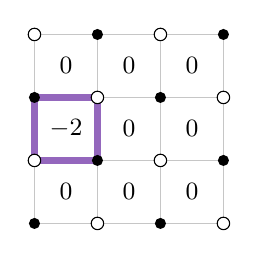
\begin{tikzpicture}[scale=0.8]
\draw[gedge] (0,0) -- (1,0);
\draw[gedge] (0,0) -- (0,1);
\draw[gedge] (0,1) -- (1,1);
\draw[gedge] (0,1) -- (0,2);
\draw[gedge] (0,2) -- (1,2);
\draw[gedge] (0,2) -- (0,3);
\draw[gedge] (0,3) -- (1,3);
\draw[gedge] (1,0) -- (2,0);
\draw[gedge] (1,0) -- (1,1);
\draw[gedge] (1,1) -- (2,1);
\draw[gedge] (1,1) -- (1,2);
\draw[gedge] (1,2) -- (2,2);
\draw[gedge] (1,2) -- (1,3);
\draw[gedge] (1,3) -- (2,3);
\draw[gedge] (2,0) -- (3,0);
\draw[gedge] (2,0) -- (2,1);
\draw[gedge] (2,1) -- (3,1);
\draw[gedge] (2,1) -- (2,2);
\draw[gedge] (2,2) -- (3,2);
\draw[gedge] (2,2) -- (2,3);
\draw[gedge] (2,3) -- (3,3);
\draw[gedge] (3,0) -- (3,1);
\draw[gedge] (3,1) -- (3,2);
\draw[gedge] (3,2) -- (3,3);
\draw[xedge] (0,1) -- (1,1);
\draw[xedge] (0,2) -- (1,2);
\draw[xedge] (0,1) -- (0,2);
\draw[xedge] (1,1) -- (1,2);
\node[pt] at (0,0) {};
\node[wpt] at (0,1) {};
\node[pt] at (0,2) {};
\node[wpt] at (0,3) {};
\node[wpt] at (1,0) {};
\node[pt] at (1,1) {};
\node[wpt] at (1,2) {};
\node[pt] at (1,3) {};
\node[pt] at (2,0) {};
\node[wpt] at (2,1) {};
\node[pt] at (2,2) {};
\node[wpt] at (2,3) {};
\node[wpt] at (3,0) {};
\node[pt] at (3,1) {};
\node[wpt] at (3,2) {};
\node[pt] at (3,3) {};
\node[taulab] at (0+0.5,0+0.5) {$0$};
\node[taulab] at (0+0.5,1+0.5) {$-2$};
\node[taulab] at (0+0.5,2+0.5) {$0$};
\node[taulab] at (1+0.5,0+0.5) {$0$};
\node[taulab] at (1+0.5,1+0.5) {$0$};
\node[taulab] at (1+0.5,2+0.5) {$0$};
\node[taulab] at (2+0.5,0+0.5) {$0$};
\node[taulab] at (2+0.5,1+0.5) {$0$};
\node[taulab] at (2+0.5,2+0.5) {$0$};
\end{tikzpicture} \\
\small (a) $F$ and $\tau_F$ & \small (b) $H$ and $\tau_H$ & \small (c) $F\oplus H$ and $D(F,H)$
\end{tabular}

\caption{(a) A Hamiltonian cycle $F$ on a $4\times4$ block, its arcs and its height $\tau_F$.
(b) The factor $H$ obtained by flipping the alternating cell $(0,1)$ of $F$, with two pieces (blue,
red), its arcs
and its height $\tau_H$.
(c) The symmetric difference $F\oplus H$ (purple), the four sides of $(0,1)$, and $D(F,H)$ in each
cell.
The only nonzero value is $-2$ at $(0,1)$, which equals $\tau_F-\tau_H$ there.}
\label{fig:D}
\end{figure}

\begin{lemma}[properties of $D$]
\label{lem:D}
Let $F,H$ be factors with the same degrees.
\begin{enumerate}
\item $D(F,H)$ is even (\lean{D\_even}).
\item $D(F,H)$ never decreases along an arc of $F$ (\lean{D\_mono\_arc}, \lean{D\_step}).
\item If $V$ is solid and $F\oplus H$ consists of edges of $V$, then $D(F,H)(c)=0$ for every
  square $c$ that is not a cell of $V$ (\lean{D\_eq\_zero\_of\_not\_cellW}).
\end{enumerate}
\end{lemma}

\begin{proof}
Part~1 holds because $D$ is a sum of weights $\pm2$.
For part~2, put $\varepsilon_F(e)=+1$ when the arc of $F$ across a unit edge $e$ points from its
lower or left square to its upper or right square, and $\varepsilon_F(e)=-1$ otherwise, and
likewise $\varepsilon_H$.
Toggling the membership of $e$ reverses its arc.
So $\varepsilon_F(e)-\varepsilon_H(e)$ is the weight of $e$ in \cref{def:D} when $e\in F\oplus H$,
and $0$ otherwise.
Going once around a point $p$, $\varepsilon_F$ adds up to $\pm(4-2\deg_F p)$ and $\varepsilon_H$ to
$\pm(4-2\deg_H p)$ with the same sign, and the two degrees are equal.
So the weights add up to $0$ around every point.
Every closed walk of squares is a sum of walks around single points, so the weights are the jumps
of a function on squares, unique once it is $0$ far left of all edges.
Reading this function along a horizontal walk from far left to $c$ crosses exactly the vertical
edges of the row of $c$ at or left of the left side of $c$, so the function is $D(F,H)$.
Hence $D(F,H)$ jumps across every side $e$ by the weight of $e$, which is $+2$ in the direction of
the arc of $F$ when $e\in F\oplus H$, and $0$ otherwise.
This proves part~2 and the statement before the lemma.

For part~3, let $c$ not be a cell of $V$, and let $m$ be a missing corner of $c$.
No edge of $F\oplus H$ meets $m$, so $D(F,H)$ is the same on the four squares at $m$.
Two king-adjacent missing points share a square, so $D(F,H)$ is the same at the squares of all
points of a king path of missing points.
As $V$ is solid, such a path joins $m$ to a point left of $V$, whose squares have no edge of
$F\oplus H$ at or left of them in their rows, so $D(F,H)=0$ there.
\end{proof}

The conclusion of part~3 is named \lean{SolidFor}~$V\ F\ H$.
Large parts of the argument use only \lean{SolidFor}, and not solidity itself.
This is what makes holes tractable in \cref{sec:classes}.

\subsection{Flips and cut cells}

\begin{definition}[alternating cell, flip]
A cell is \emph{alternating} in $H$ when two opposite sides are dark and the other two are light
(Lean \lean{Alt}).
The \emph{flip} of a cell toggles its four sides (Lean \lean{flip}).
\end{definition}

A cell is alternating exactly when its four arcs all point out or all point in
(\lean{alt\_iff\_uniform}).
So an alternating cell is a local minimum or maximum of the height.
Flipping it keeps every degree, reverses its four arcs, and changes its height by $\pm2$.

\begin{definition}[cut cell, merging cell]
A cell is a \emph{cut cell} of $H$ when its four corners do not all lie in one piece (Lean
\lean{CutSq}).
A \emph{merging cell} is an alternating cut cell.
\end{definition}

Flipping a merging cell joins the two pieces at its two dark sides, so the number of pieces drops by
one.
Flipping an alternating cell that is not cut splits a piece or keeps the count.
\Cref{fig:flip} shows a merging flip.

\begin{figure}[t]
\centering
% SPDX-License-Identifier: CC0-1.0
% Generated by gen.py; do not edit by hand.
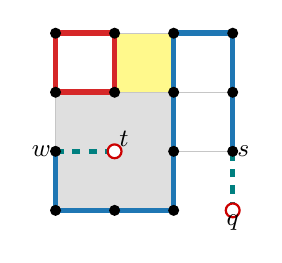
\begin{tikzpicture}[scale=0.75]
\fill[holecell] (0,0) rectangle (1,1);
\fill[holecell] (1,0) rectangle (2,1);
\fill[holecell] (0,1) rectangle (1,2);
\fill[holecell] (1,1) rectangle (2,2);
\fill[hicell] (1,2) rectangle (2,3);
\draw[gedge] (0,0) -- (1,0);
\draw[gedge] (0,0) -- (0,1);
\draw[gedge] (0,1) -- (0,2);
\draw[gedge] (0,2) -- (1,2);
\draw[gedge] (0,2) -- (0,3);
\draw[gedge] (0,3) -- (1,3);
\draw[gedge] (1,0) -- (2,0);
\draw[gedge] (1,2) -- (2,2);
\draw[gedge] (1,2) -- (1,3);
\draw[gedge] (1,3) -- (2,3);
\draw[gedge] (2,0) -- (2,1);
\draw[gedge] (2,1) -- (3,1);
\draw[gedge] (2,1) -- (2,2);
\draw[gedge] (2,2) -- (3,2);
\draw[gedge] (2,2) -- (2,3);
\draw[gedge] (2,3) -- (3,3);
\draw[gedge] (3,1) -- (3,2);
\draw[gedge] (3,2) -- (3,3);
\draw[pc1] (0,0) -- (0,1);
\draw[pc1] (0,0) -- (1,0);
\draw[pc1] (1,0) -- (2,0);
\draw[pc1] (2,0) -- (2,1);
\draw[pc1] (2,1) -- (2,2);
\draw[pc1] (2,2) -- (2,3);
\draw[pc1] (2,3) -- (3,3);
\draw[pc1] (3,2) -- (3,3);
\draw[pc1] (3,1) -- (3,2);
\draw[pc2] (0,2) -- (1,2);
\draw[pc2] (1,2) -- (1,3);
\draw[pc2] (0,3) -- (1,3);
\draw[pc2] (0,2) -- (0,3);
\draw[ph] (0,1) -- (1,1);
\draw[ph] (3,0) -- (3,1);
\node[pt] at (0,0) {};
\node[pt] at (0,1) {};
\node[pt] at (0,2) {};
\node[pt] at (0,3) {};
\node[pt] at (1,0) {};
\node[pt] at (1,2) {};
\node[pt] at (1,3) {};
\node[pt] at (2,0) {};
\node[pt] at (2,1) {};
\node[pt] at (2,2) {};
\node[pt] at (2,3) {};
\node[pt] at (3,1) {};
\node[pt] at (3,2) {};
\node[pt] at (3,3) {};
\node[miss] at (1,1) {};
\node[miss] at (3,0) {};
\node[lab,above right] at (1,1) {$t$};
\node[lab,below] at (3,0) {$q$};
\node[lab,left] at (0,1) {$w$};
\node[lab,right] at (3,1) {$s$};
\end{tikzpicture}\qquad
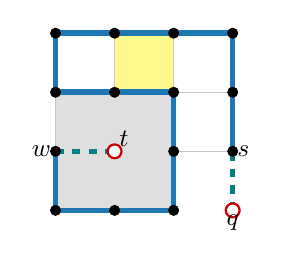
\begin{tikzpicture}[scale=0.75]
\fill[holecell] (0,0) rectangle (1,1);
\fill[holecell] (1,0) rectangle (2,1);
\fill[holecell] (0,1) rectangle (1,2);
\fill[holecell] (1,1) rectangle (2,2);
\fill[hicell] (1,2) rectangle (2,3);
\draw[gedge] (0,0) -- (1,0);
\draw[gedge] (0,0) -- (0,1);
\draw[gedge] (0,1) -- (0,2);
\draw[gedge] (0,2) -- (1,2);
\draw[gedge] (0,2) -- (0,3);
\draw[gedge] (0,3) -- (1,3);
\draw[gedge] (1,0) -- (2,0);
\draw[gedge] (1,2) -- (2,2);
\draw[gedge] (1,2) -- (1,3);
\draw[gedge] (1,3) -- (2,3);
\draw[gedge] (2,0) -- (2,1);
\draw[gedge] (2,1) -- (3,1);
\draw[gedge] (2,1) -- (2,2);
\draw[gedge] (2,2) -- (3,2);
\draw[gedge] (2,2) -- (2,3);
\draw[gedge] (2,3) -- (3,3);
\draw[gedge] (3,1) -- (3,2);
\draw[gedge] (3,2) -- (3,3);
\draw[pc1] (0,0) -- (0,1);
\draw[pc1] (0,0) -- (1,0);
\draw[pc1] (1,0) -- (2,0);
\draw[pc1] (2,0) -- (2,1);
\draw[pc1] (2,1) -- (2,2);
\draw[pc1] (1,2) -- (2,2);
\draw[pc1] (0,2) -- (1,2);
\draw[pc1] (0,2) -- (0,3);
\draw[pc1] (0,3) -- (1,3);
\draw[pc1] (1,3) -- (2,3);
\draw[pc1] (2,3) -- (3,3);
\draw[pc1] (3,2) -- (3,3);
\draw[pc1] (3,1) -- (3,2);
\draw[ph] (0,1) -- (1,1);
\draw[ph] (3,0) -- (3,1);
\node[pt] at (0,0) {};
\node[pt] at (0,1) {};
\node[pt] at (0,2) {};
\node[pt] at (0,3) {};
\node[pt] at (1,0) {};
\node[pt] at (1,2) {};
\node[pt] at (1,3) {};
\node[pt] at (2,0) {};
\node[pt] at (2,1) {};
\node[pt] at (2,2) {};
\node[pt] at (2,3) {};
\node[pt] at (3,1) {};
\node[pt] at (3,2) {};
\node[pt] at (3,3) {};
\node[miss] at (1,1) {};
\node[miss] at (3,0) {};
\node[lab,above right] at (1,1) {$t$};
\node[lab,below] at (3,0) {$q$};
\node[lab,left] at (0,1) {$w$};
\node[lab,right] at (3,1) {$s$};
\end{tikzpicture}

\caption{A flip joining two pieces, from the $4\times4$ instance of \cref{sec:inside}.
Left: a factor with two pieces, a path (blue) and a $4$-cycle (red).
The yellow cell is alternating and cut, so it is a merging cell.
Right: after the flip, one piece.
Grey squares are the four hole cells around the deleted inner endpoint $t$ (\cref{sec:vortex}).
Dashed edges are phantom edges.}
\label{fig:flip}
\end{figure}

% =====================================================================
\section{Sheffield's phase and the certificate}
\label{sec:sheffield}

This section describes the cycle algorithm of~\cite[\S4]{sheffield2000} in the form used in Lean.
In the Lean development a factor lives on a set $W\supseteq V$.
Only cells of $V$ are flipped.
Every corner of a cell of $V$ has degree $2$ (in \cref{sec:phantom} this is arranged for path
factors).

\subsection{Frames, critical cells and rows}

\begin{definition}[frame]
A \emph{frame} of a cell $c$ is a choice of one of its sides as the \emph{front}.
The opposite side is the \emph{back}, and the other two are the \emph{laterals}.
The corners on the back are $b_1,b_2$ and those on the front are $f_1,f_2$, with laterals
$b_1f_1$ and $b_2f_2$ (Lean \lean{back}, \lean{front}, \lean{lat1}, \lean{back1}, \lean{front1} in
\lean{Algorithm.lean}, \lean{lat2} in \lean{Strip.lean}).
The $j$-th cell of the strip from $c$ in the direction of its front is $c_j$, with $c_0=c$ (Lean
\lean{cellJ}).
\end{definition}

\begin{definition}[critical cell, corner cell]
\label{def:critical}
A cell $c$ is \emph{critical} in a frame when $b_1,b_2$ lie in one piece, $f_1,f_2$ lie in one
piece, these two pieces differ, and exactly one of back and front is dark (Lean
\lean{CriticalIn}).
A cell is a \emph{corner cell} when one corner is alone in its piece among the four corners, the
other three share a piece, and the two sides at the corner opposite the lone corner are dark
(Lean \lean{CornerIn}).
\end{definition}

\begin{figure}[t]
\centering
% SPDX-License-Identifier: CC0-1.0
% Generated by gen.py; do not edit by hand.
\begin{tabular}{c@{\qquad}c@{\qquad}c}
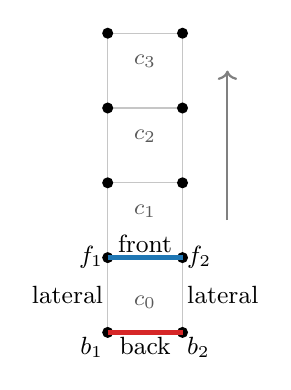
\begin{tikzpicture}[scale=0.95]
\draw[gedge] (0,0) -- (1,0);
\draw[gedge] (0,0) -- (0,1);
\draw[gedge] (0,1) -- (1,1);
\draw[gedge] (0,1) -- (0,2);
\draw[gedge] (0,2) -- (1,2);
\draw[gedge] (0,2) -- (0,3);
\draw[gedge] (0,3) -- (1,3);
\draw[gedge] (0,3) -- (0,4);
\draw[gedge] (0,4) -- (1,4);
\draw[gedge] (1,0) -- (1,1);
\draw[gedge] (1,1) -- (1,2);
\draw[gedge] (1,2) -- (1,3);
\draw[gedge] (1,3) -- (1,4);
\node[pt] at (0,0) {};
\node[pt] at (0,1) {};
\node[pt] at (0,2) {};
\node[pt] at (0,3) {};
\node[pt] at (0,4) {};
\node[pt] at (1,0) {};
\node[pt] at (1,1) {};
\node[pt] at (1,2) {};
\node[pt] at (1,3) {};
\node[pt] at (1,4) {};
\draw[pcB,line width=2pt] (0,0) -- (1,0);
\draw[pcA,line width=2pt] (0,1) -- (1,1);
\node[lab,below] at (0.5,0) {back};
\node[lab,above] at (0.5,1) {front};
\node[lab,left] at (0,0.5) {lateral};
\node[lab,right] at (1,0.5) {lateral};
\node[lab,below left] at (0,0) {$b_1$};
\node[lab,below right] at (1,0) {$b_2$};
\node[lab,left] at (0,1) {$f_1$};
\node[lab,right] at (1,1) {$f_2$};
\node[cellname] at (0.5,0+0.4) {$c_0$};
\node[cellname] at (0.5,1+0.62) {$c_1$};
\node[cellname] at (0.5,2+0.62) {$c_2$};
\node[cellname] at (0.5,3+0.62) {$c_3$};
\draw[->,thick,gray] (1.6,1.5) -- (1.6,3.5);
\end{tikzpicture} & 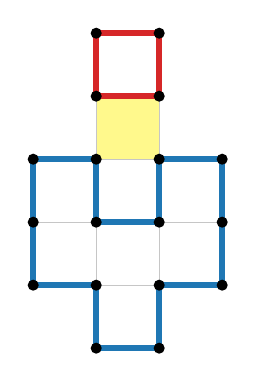
\begin{tikzpicture}[scale=0.8]
\fill[hicell] (1,4) rectangle (2,5);
\draw[gedge] (0,2) -- (1,2);
\draw[gedge] (0,2) -- (0,3);
\draw[gedge] (0,3) -- (1,3);
\draw[gedge] (0,3) -- (0,4);
\draw[gedge] (0,4) -- (1,4);
\draw[gedge] (1,1) -- (2,1);
\draw[gedge] (1,1) -- (1,2);
\draw[gedge] (1,2) -- (2,2);
\draw[gedge] (1,2) -- (1,3);
\draw[gedge] (1,3) -- (2,3);
\draw[gedge] (1,3) -- (1,4);
\draw[gedge] (1,4) -- (2,4);
\draw[gedge] (1,4) -- (1,5);
\draw[gedge] (1,5) -- (2,5);
\draw[gedge] (1,5) -- (1,6);
\draw[gedge] (1,6) -- (2,6);
\draw[gedge] (2,1) -- (2,2);
\draw[gedge] (2,2) -- (3,2);
\draw[gedge] (2,2) -- (2,3);
\draw[gedge] (2,3) -- (3,3);
\draw[gedge] (2,3) -- (2,4);
\draw[gedge] (2,4) -- (3,4);
\draw[gedge] (2,4) -- (2,5);
\draw[gedge] (2,5) -- (2,6);
\draw[gedge] (3,2) -- (3,3);
\draw[gedge] (3,3) -- (3,4);
\draw[pc1] (0,2) -- (1,2);
\draw[pc1] (0,4) -- (1,4);
\draw[pc1] (1,1) -- (2,1);
\draw[pc1] (1,3) -- (2,3);
\draw[pc1] (2,2) -- (3,2);
\draw[pc1] (2,4) -- (3,4);
\draw[pc1] (0,2) -- (0,3);
\draw[pc1] (0,3) -- (0,4);
\draw[pc1] (1,1) -- (1,2);
\draw[pc1] (1,3) -- (1,4);
\draw[pc1] (2,1) -- (2,2);
\draw[pc1] (2,3) -- (2,4);
\draw[pc1] (3,2) -- (3,3);
\draw[pc1] (3,3) -- (3,4);
\draw[pc2] (1,5) -- (2,5);
\draw[pc2] (1,6) -- (2,6);
\draw[pc2] (1,5) -- (1,6);
\draw[pc2] (2,5) -- (2,6);
\node[pt] at (0,2) {};
\node[pt] at (0,3) {};
\node[pt] at (0,4) {};
\node[pt] at (1,1) {};
\node[pt] at (1,2) {};
\node[pt] at (1,3) {};
\node[pt] at (1,4) {};
\node[pt] at (1,5) {};
\node[pt] at (1,6) {};
\node[pt] at (2,1) {};
\node[pt] at (2,2) {};
\node[pt] at (2,3) {};
\node[pt] at (2,4) {};
\node[pt] at (2,5) {};
\node[pt] at (2,6) {};
\node[pt] at (3,2) {};
\node[pt] at (3,3) {};
\node[pt] at (3,4) {};
\end{tikzpicture} & 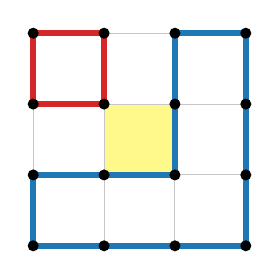
\begin{tikzpicture}[scale=0.9]
\fill[hicell] (1,1) rectangle (2,2);
\draw[gedge] (0,0) -- (1,0);
\draw[gedge] (0,0) -- (0,1);
\draw[gedge] (0,1) -- (1,1);
\draw[gedge] (0,1) -- (0,2);
\draw[gedge] (0,2) -- (1,2);
\draw[gedge] (0,2) -- (0,3);
\draw[gedge] (0,3) -- (1,3);
\draw[gedge] (1,0) -- (2,0);
\draw[gedge] (1,0) -- (1,1);
\draw[gedge] (1,1) -- (2,1);
\draw[gedge] (1,1) -- (1,2);
\draw[gedge] (1,2) -- (2,2);
\draw[gedge] (1,2) -- (1,3);
\draw[gedge] (1,3) -- (2,3);
\draw[gedge] (2,0) -- (3,0);
\draw[gedge] (2,0) -- (2,1);
\draw[gedge] (2,1) -- (3,1);
\draw[gedge] (2,1) -- (2,2);
\draw[gedge] (2,2) -- (3,2);
\draw[gedge] (2,2) -- (2,3);
\draw[gedge] (2,3) -- (3,3);
\draw[gedge] (3,0) -- (3,1);
\draw[gedge] (3,1) -- (3,2);
\draw[gedge] (3,2) -- (3,3);
\draw[pc1] (0,0) -- (1,0);
\draw[pc1] (0,1) -- (1,1);
\draw[pc1] (1,0) -- (2,0);
\draw[pc1] (1,1) -- (2,1);
\draw[pc1] (2,0) -- (3,0);
\draw[pc1] (2,3) -- (3,3);
\draw[pc1] (0,0) -- (0,1);
\draw[pc1] (2,1) -- (2,2);
\draw[pc1] (2,2) -- (2,3);
\draw[pc1] (3,0) -- (3,1);
\draw[pc1] (3,1) -- (3,2);
\draw[pc1] (3,2) -- (3,3);
\draw[pc2] (0,2) -- (1,2);
\draw[pc2] (0,3) -- (1,3);
\draw[pc2] (0,2) -- (0,3);
\draw[pc2] (1,2) -- (1,3);
\node[pt] at (0,0) {};
\node[pt] at (0,1) {};
\node[pt] at (0,2) {};
\node[pt] at (0,3) {};
\node[pt] at (1,0) {};
\node[pt] at (1,1) {};
\node[pt] at (1,2) {};
\node[pt] at (1,3) {};
\node[pt] at (2,0) {};
\node[pt] at (2,1) {};
\node[pt] at (2,2) {};
\node[pt] at (2,3) {};
\node[pt] at (3,0) {};
\node[pt] at (3,1) {};
\node[pt] at (3,2) {};
\node[pt] at (3,3) {};
\end{tikzpicture} \\
\small (a) a frame & \small (b) a critical cell & \small (c) a corner cell
\end{tabular}

\caption{(a) A frame of the cell $c_0$ with its front up, the corners $b_1,b_2,f_1,f_2$, and the strip
$c_0,c_1,c_2,c_3$ in the direction of the front.
(b) A critical cell (yellow) in a plus-shaped set with a factor of two pieces (blue, red).
Its back, the top side, is dark and lies on the red $4$-cycle.
Its front, the bottom side, is light, and its front corners lie on the blue cycle.
(c) A corner cell (yellow) in a $4\times4$ block.
Its top-left corner is alone in its piece among the four corners.
The two sides at the opposite corner, the bottom-right one, are dark.}
\label{fig:frame}
\end{figure}

Sheffield's Lemma~1 says the following.
If no cut cell is alternating, then every cut cell is critical or a corner cell, and no cell
touches three pieces.
The proof uses degree $2$ at the corners.
In Lean the cut-cell shapes are in \lean{Shapes.lean} and \lean{E1.lean}.
At a degree-one point near the cells the lemma has exceptions.
One of them is a cell with the \emph{E1 shape}.
In some frame its back corners share a piece, each front corner is alone in its own piece, one front
corner is an out-vertex (\cref{def:far}), and the square in front is not a cell (Lean
\lean{TriShape}).
A cell has the \emph{diagonal shape} when no side has both corners in one piece but two diagonal
corners do (Lean \lean{DiagShape}).

\begin{definition}[row, stuck]
\label{def:row}
Let $q$ be critical in a frame with dark back.
The \emph{row} from $q$ runs through $q=c_0,c_1,\dots$ while the arc across the front of each cell
points the same way as at $q$.
Its last cell $c_{r-1}$ is the first one whose front arc points the other way.
The row is \emph{well formed} when $c_1,\dots,c_{r-1}$ are cells of $V$ and are not cut.
The cell $q$ is \emph{stuck} when the run reaches a square $c_k$ ($k\ge1$) that is not a cell or is
a cut cell before its arc turns (Lean \lean{StuckAt}, \lean{ColProof.lean}).
\end{definition}

The heights rise strictly along the row (or fall strictly, depending on the direction of the
arcs).
The last cell is a local maximum (or minimum) along the row.
\Cref{fig:row} shows a row of odd length and a stuck cell, with the heights drawn in.

\begin{figure}[t]
\centering
% SPDX-License-Identifier: CC0-1.0
% Generated by gen.py; do not edit by hand.
\begin{tabular}{c@{\qquad}c}
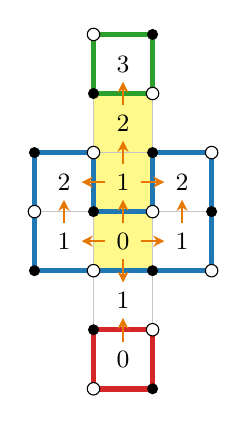
\begin{tikzpicture}[scale=0.75]
\fill[hicell] (1,4) rectangle (2,5);
\fill[hicell] (1,3) rectangle (2,4);
\fill[hicell] (1,2) rectangle (2,3);
\draw[gedge] (0,2) -- (1,2);
\draw[gedge] (0,2) -- (0,3);
\draw[gedge] (0,3) -- (1,3);
\draw[gedge] (0,3) -- (0,4);
\draw[gedge] (0,4) -- (1,4);
\draw[gedge] (1,0) -- (2,0);
\draw[gedge] (1,0) -- (1,1);
\draw[gedge] (1,1) -- (2,1);
\draw[gedge] (1,1) -- (1,2);
\draw[gedge] (1,2) -- (2,2);
\draw[gedge] (1,2) -- (1,3);
\draw[gedge] (1,3) -- (2,3);
\draw[gedge] (1,3) -- (1,4);
\draw[gedge] (1,4) -- (2,4);
\draw[gedge] (1,4) -- (1,5);
\draw[gedge] (1,5) -- (2,5);
\draw[gedge] (1,5) -- (1,6);
\draw[gedge] (1,6) -- (2,6);
\draw[gedge] (2,0) -- (2,1);
\draw[gedge] (2,1) -- (2,2);
\draw[gedge] (2,2) -- (3,2);
\draw[gedge] (2,2) -- (2,3);
\draw[gedge] (2,3) -- (3,3);
\draw[gedge] (2,3) -- (2,4);
\draw[gedge] (2,4) -- (3,4);
\draw[gedge] (2,4) -- (2,5);
\draw[gedge] (2,5) -- (2,6);
\draw[gedge] (3,2) -- (3,3);
\draw[gedge] (3,3) -- (3,4);
\draw[pc1] (0,2) -- (1,2);
\draw[pc1] (0,4) -- (1,4);
\draw[pc1] (1,2) -- (2,2);
\draw[pc1] (1,3) -- (2,3);
\draw[pc1] (2,2) -- (3,2);
\draw[pc1] (2,4) -- (3,4);
\draw[pc1] (0,2) -- (0,3);
\draw[pc1] (0,3) -- (0,4);
\draw[pc1] (1,3) -- (1,4);
\draw[pc1] (2,3) -- (2,4);
\draw[pc1] (3,2) -- (3,3);
\draw[pc1] (3,3) -- (3,4);
\draw[pc2] (1,0) -- (2,0);
\draw[pc2] (1,1) -- (2,1);
\draw[pc2] (1,0) -- (1,1);
\draw[pc2] (2,0) -- (2,1);
\draw[pc3] (1,5) -- (2,5);
\draw[pc3] (1,6) -- (2,6);
\draw[pc3] (1,5) -- (1,6);
\draw[pc3] (2,5) -- (2,6);
\node[pt] at (0,2) {};
\node[wpt] at (0,3) {};
\node[pt] at (0,4) {};
\node[wpt] at (1,0) {};
\node[pt] at (1,1) {};
\node[wpt] at (1,2) {};
\node[pt] at (1,3) {};
\node[wpt] at (1,4) {};
\node[pt] at (1,5) {};
\node[wpt] at (1,6) {};
\node[pt] at (2,0) {};
\node[wpt] at (2,1) {};
\node[pt] at (2,2) {};
\node[wpt] at (2,3) {};
\node[pt] at (2,4) {};
\node[wpt] at (2,5) {};
\node[pt] at (2,6) {};
\node[wpt] at (3,2) {};
\node[pt] at (3,3) {};
\node[wpt] at (3,4) {};
\draw[arcarrow] (0.50,2.80) -- (0.50,3.20);
\draw[arcarrow] (1.20,2.50) -- (0.80,2.50);
\draw[arcarrow] (1.20,3.50) -- (0.80,3.50);
\draw[arcarrow] (1.50,0.80) -- (1.50,1.20);
\draw[arcarrow] (1.50,2.20) -- (1.50,1.80);
\draw[arcarrow] (1.50,2.80) -- (1.50,3.20);
\draw[arcarrow] (1.80,2.50) -- (2.20,2.50);
\draw[arcarrow] (1.50,3.80) -- (1.50,4.20);
\draw[arcarrow] (1.80,3.50) -- (2.20,3.50);
\draw[arcarrow] (1.50,4.80) -- (1.50,5.20);
\draw[arcarrow] (2.50,2.80) -- (2.50,3.20);
\node[taulab] at (0+0.5,2+0.5) {$1$};
\node[taulab] at (0+0.5,3+0.5) {$2$};
\node[taulab] at (1+0.5,0+0.5) {$0$};
\node[taulab] at (1+0.5,1+0.5) {$1$};
\node[taulab] at (1+0.5,2+0.5) {$0$};
\node[taulab] at (1+0.5,3+0.5) {$1$};
\node[taulab] at (1+0.5,4+0.5) {$2$};
\node[taulab] at (1+0.5,5+0.5) {$3$};
\node[taulab] at (2+0.5,2+0.5) {$1$};
\node[taulab] at (2+0.5,3+0.5) {$2$};
\end{tikzpicture} & 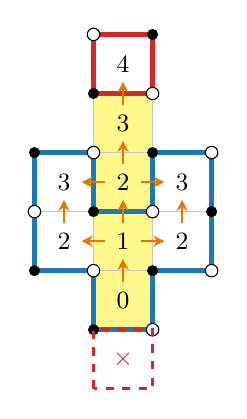
\begin{tikzpicture}[scale=0.75]
\fill[hicell] (1,4) rectangle (2,5);
\fill[hicell] (1,3) rectangle (2,4);
\fill[hicell] (1,2) rectangle (2,3);
\fill[hicell] (1,1) rectangle (2,2);
\draw[gedge] (0,2) -- (1,2);
\draw[gedge] (0,2) -- (0,3);
\draw[gedge] (0,3) -- (1,3);
\draw[gedge] (0,3) -- (0,4);
\draw[gedge] (0,4) -- (1,4);
\draw[gedge] (1,1) -- (2,1);
\draw[gedge] (1,1) -- (1,2);
\draw[gedge] (1,2) -- (2,2);
\draw[gedge] (1,2) -- (1,3);
\draw[gedge] (1,3) -- (2,3);
\draw[gedge] (1,3) -- (1,4);
\draw[gedge] (1,4) -- (2,4);
\draw[gedge] (1,4) -- (1,5);
\draw[gedge] (1,5) -- (2,5);
\draw[gedge] (1,5) -- (1,6);
\draw[gedge] (1,6) -- (2,6);
\draw[gedge] (2,1) -- (2,2);
\draw[gedge] (2,2) -- (3,2);
\draw[gedge] (2,2) -- (2,3);
\draw[gedge] (2,3) -- (3,3);
\draw[gedge] (2,3) -- (2,4);
\draw[gedge] (2,4) -- (3,4);
\draw[gedge] (2,4) -- (2,5);
\draw[gedge] (2,5) -- (2,6);
\draw[gedge] (3,2) -- (3,3);
\draw[gedge] (3,3) -- (3,4);
\draw[pc1] (0,2) -- (1,2);
\draw[pc1] (0,4) -- (1,4);
\draw[pc1] (1,1) -- (2,1);
\draw[pc1] (1,3) -- (2,3);
\draw[pc1] (2,2) -- (3,2);
\draw[pc1] (2,4) -- (3,4);
\draw[pc1] (0,2) -- (0,3);
\draw[pc1] (0,3) -- (0,4);
\draw[pc1] (1,1) -- (1,2);
\draw[pc1] (1,3) -- (1,4);
\draw[pc1] (2,1) -- (2,2);
\draw[pc1] (2,3) -- (2,4);
\draw[pc1] (3,2) -- (3,3);
\draw[pc1] (3,3) -- (3,4);
\draw[pc2] (1,5) -- (2,5);
\draw[pc2] (1,6) -- (2,6);
\draw[pc2] (1,5) -- (1,6);
\draw[pc2] (2,5) -- (2,6);
\node[pt] at (0,2) {};
\node[wpt] at (0,3) {};
\node[pt] at (0,4) {};
\node[pt] at (1,1) {};
\node[wpt] at (1,2) {};
\node[pt] at (1,3) {};
\node[wpt] at (1,4) {};
\node[pt] at (1,5) {};
\node[wpt] at (1,6) {};
\node[wpt] at (2,1) {};
\node[pt] at (2,2) {};
\node[wpt] at (2,3) {};
\node[pt] at (2,4) {};
\node[wpt] at (2,5) {};
\node[pt] at (2,6) {};
\node[wpt] at (3,2) {};
\node[pt] at (3,3) {};
\node[wpt] at (3,4) {};
\draw[arcarrow] (0.50,2.80) -- (0.50,3.20);
\draw[arcarrow] (1.20,2.50) -- (0.80,2.50);
\draw[arcarrow] (1.20,3.50) -- (0.80,3.50);
\draw[arcarrow] (1.50,1.80) -- (1.50,2.20);
\draw[arcarrow] (1.50,2.80) -- (1.50,3.20);
\draw[arcarrow] (1.80,2.50) -- (2.20,2.50);
\draw[arcarrow] (1.50,3.80) -- (1.50,4.20);
\draw[arcarrow] (1.80,3.50) -- (2.20,3.50);
\draw[arcarrow] (1.50,4.80) -- (1.50,5.20);
\draw[arcarrow] (2.50,2.80) -- (2.50,3.20);
\node[taulab] at (0+0.5,2+0.5) {$2$};
\node[taulab] at (0+0.5,3+0.5) {$3$};
\node[taulab] at (1+0.5,1+0.5) {$0$};
\node[taulab] at (1+0.5,2+0.5) {$1$};
\node[taulab] at (1+0.5,3+0.5) {$2$};
\node[taulab] at (1+0.5,4+0.5) {$3$};
\node[taulab] at (1+0.5,5+0.5) {$4$};
\node[taulab] at (2+0.5,2+0.5) {$2$};
\node[taulab] at (2+0.5,3+0.5) {$3$};
\draw[pcB,very thick,dashed] (1,0) rectangle (2,1);
\node[lab,pcB] at (1+0.5,0+0.5) {$\times$};
\end{tikzpicture} \\
\small (a) a row of length $3$ & \small (b) a stuck cell, heights drawn
\end{tabular}

\caption{Rows in plus-shaped sets, with the arcs (orange) and a height in every cell.
(a) A factor with three pieces.
The cell $(1,4)$ is critical in the frame whose front is its bottom side.
Its row (yellow) is $(1,4),(1,3),(1,2)$, of length $3$.
The heights fall $2,1,0$ along it, so the arc across the front of each of its cells except the last
points up.
The arc across the front of $(1,2)$ points down, from height $0$ to height $1$, so the row ends at
$(1,2)$.
(b) The same shape without its two bottom points, and a factor with two pieces.
The row from $(1,4)$ falls $3,2,1,0$ through four cells (yellow), and the next square, $(1,0)$
(red cross), is not a cell of $V$.
So $(1,4)$ is stuck.
It is the only critical cell, the factor has no merging cell, and the phase ends stuck.
By the certificate (\cref{thm:cert}) this set has no Hamiltonian cycle.}
\label{fig:row}
\end{figure}

\begin{definition}[bridge, fixed pair]
\label{def:bridge}
A \emph{bridge step} applies to a well formed row of even length $r\ge2$ from a critical cell $q$
that is not a bridge square of an earlier bridge (Lean \lean{RowStep}, \lean{Bridges.lean}).
It flips only the last cell $E=c_{r-1}$, and it requires that this flip splits a piece
(\lean{RowStep.split}).
The cells $c_0,\dots,c_{r-1}$ of the row are the \emph{bridge squares}.
The two last cells $(A,E)=(c_{r-2},c_{r-1})$ form the \emph{fixed pair} of the bridge (Lean
\lean{FixedPr}, \lean{Bridge.pairOf}), and they are its \emph{pair squares}.
\end{definition}

\begin{figure}[t]
\centering
% SPDX-License-Identifier: CC0-1.0
% Generated by gen.py; do not edit by hand.
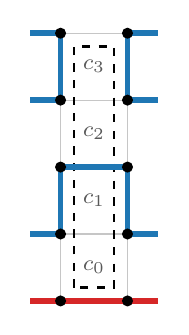
\begin{tikzpicture}[scale=0.85]
\draw[gedge] (0,0) -- (1,0);
\draw[gedge] (0,0) -- (0,1);
\draw[gedge] (0,1) -- (1,1);
\draw[gedge] (0,1) -- (0,2);
\draw[gedge] (0,2) -- (1,2);
\draw[gedge] (0,2) -- (0,3);
\draw[gedge] (0,3) -- (1,3);
\draw[gedge] (0,3) -- (0,4);
\draw[gedge] (0,4) -- (1,4);
\draw[gedge] (1,0) -- (1,1);
\draw[gedge] (1,1) -- (1,2);
\draw[gedge] (1,2) -- (1,3);
\draw[gedge] (1,3) -- (1,4);
\draw[rowbox] (0.2,0.2) rectangle (0.8,3.8);
\draw[pc2] (0,0) -- (1,0);
\draw[pc2,stub] (0,0) -- (-0.45,0);
\draw[pc2,stub] (1,0) -- (1.45,0);
\draw[pc1,stub] (0,1) -- (-0.45,1);
\draw[pc1,stub] (1,1) -- (1.45,1);
\draw[pc1,stub] (0,3) -- (-0.45,3);
\draw[pc1,stub] (1,3) -- (1.45,3);
\draw[pc1] (0,1) -- (0,2);
\draw[pc1] (1,1) -- (1,2);
\draw[pc1] (0,2) -- (1,2);
\draw[pc1] (0,3) -- (0,4);
\draw[pc1] (1,3) -- (1,4);
\draw[pc1,stub] (0,4) -- (-0.45,4);
\draw[pc1,stub] (1,4) -- (1.45,4);
\node[pt] at (0,0) {};
\node[pt] at (0,1) {};
\node[pt] at (0,2) {};
\node[pt] at (0,3) {};
\node[pt] at (0,4) {};
\node[pt] at (1,0) {};
\node[pt] at (1,1) {};
\node[pt] at (1,2) {};
\node[pt] at (1,3) {};
\node[pt] at (1,4) {};
\node[cellname] at (0.5,0+0.5) {$c_0$};
\node[cellname] at (0.5,1+0.5) {$c_1$};
\node[cellname] at (0.5,2+0.5) {$c_2$};
\node[cellname] at (0.5,3+0.5) {$c_3$};
\end{tikzpicture}\qquad\qquad
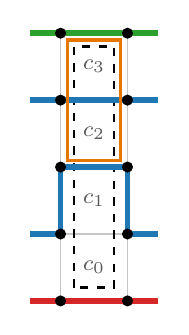
\begin{tikzpicture}[scale=0.85]
\draw[gedge] (0,0) -- (1,0);
\draw[gedge] (0,0) -- (0,1);
\draw[gedge] (0,1) -- (1,1);
\draw[gedge] (0,1) -- (0,2);
\draw[gedge] (0,2) -- (1,2);
\draw[gedge] (0,2) -- (0,3);
\draw[gedge] (0,3) -- (1,3);
\draw[gedge] (0,3) -- (0,4);
\draw[gedge] (0,4) -- (1,4);
\draw[gedge] (1,0) -- (1,1);
\draw[gedge] (1,1) -- (1,2);
\draw[gedge] (1,2) -- (1,3);
\draw[gedge] (1,3) -- (1,4);
\draw[rowbox] (0.2,0.2) rectangle (0.8,3.8);
\draw[pc2] (0,0) -- (1,0);
\draw[pc2,stub] (0,0) -- (-0.45,0);
\draw[pc2,stub] (1,0) -- (1.45,0);
\draw[pc1,stub] (0,1) -- (-0.45,1);
\draw[pc1,stub] (1,1) -- (1.45,1);
\draw[pc1,stub] (0,3) -- (-0.45,3);
\draw[pc1,stub] (1,3) -- (1.45,3);
\draw[pc1] (0,1) -- (0,2);
\draw[pc1] (1,1) -- (1,2);
\draw[pc1] (0,2) -- (1,2);
\draw[pc1] (0,3) -- (1,3);
\draw[pc3] (0,4) -- (1,4);
\draw[pc3,stub] (0,4) -- (-0.45,4);
\draw[pc3,stub] (1,4) -- (1.45,4);
\node[pt] at (0,0) {};
\node[pt] at (0,1) {};
\node[pt] at (0,2) {};
\node[pt] at (0,3) {};
\node[pt] at (0,4) {};
\node[pt] at (1,0) {};
\node[pt] at (1,1) {};
\node[pt] at (1,2) {};
\node[pt] at (1,3) {};
\node[pt] at (1,4) {};
\node[cellname] at (0.5,0+0.5) {$c_0$};
\node[cellname] at (0.5,1+0.5) {$c_1$};
\node[cellname] at (0.5,2+0.5) {$c_2$};
\node[cellname] at (0.5,3+0.5) {$c_3$};
\draw[pairbox] (0.1,2.1) rectangle (0.9,3.9);
\end{tikzpicture}

\caption{An even row $c_0,\dots,c_3$ of length $r=4$ upward from a critical cell $c_0$, and the bridge
made from it.
The dashed box is the row.
The window shows the edges forced by the bridge pattern (\lean{RegionOK}).
Short stubs are edges that leave the window.
Left: before the step, $c_0$ has a dark back (red piece below) and the strip pattern above it
(blue piece).
The last cell $E=c_3$ has dark laterals and light back and front.
Right: $E$ is flipped.
Its back and front are now dark.
The strand through its top corners has split off from the blue piece (green).
Which of the two strands keeps the blue piece depends on edges outside the window, and the
colouring shows one possibility.
The orange box marks the fixed pair $(c_2,c_3)$.}
\label{fig:bridge}
\end{figure}

\subsection{The phase}

A \emph{phase} starts from a factor $H_0$ with $m$ pieces and no bridges.
It repeats the following test in a state $H$ with a list of bridges (Lean \lean{phase},
\lean{SPhaseAlg.lean}).
\begin{enumerate}
\item If some merging cell is not a square of a fixed pair, the phase ends with outcome
  \emph{merge}.
\item Otherwise it looks for a critical cell with dark back that is not stuck and not a bridge square.
  If none exists, the phase ends with outcome \emph{stuck}.
\item If that cell's row has odd length, the phase ends with outcome \emph{odd}.
\item If the row has even length and flipping its last cell splits a piece, the phase makes a
  bridge step and continues.
\item If the row has even length and flipping its last cell does not split, the phase ends with
  outcome \emph{twist}.
\end{enumerate}
Each bridge step adds one piece, so a state reached after $k$ steps has $m+k$ pieces
(\lean{reach\_count}, \lean{PhaseCount.lean}, \cref{app:step}).
The case split is exhaustive (\lean{phase\_spec}).
\Cref{fig:phase} shows each outcome on a small factor, and \cref{app:runs} follows two complete
runs with their heights.

\begin{figure}[!htbp]
\centering
% SPDX-License-Identifier: CC0-1.0
% Generated by gen.py; do not edit by hand.
\begin{tabular}{c@{\qquad}c@{\qquad}c}
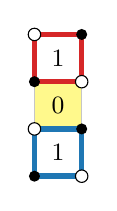
\begin{tikzpicture}[scale=0.6]
\fill[hicell] (0,1) rectangle (1,2);
\draw[gedge] (0,0) -- (1,0);
\draw[gedge] (0,0) -- (0,1);
\draw[gedge] (0,1) -- (1,1);
\draw[gedge] (0,1) -- (0,2);
\draw[gedge] (0,2) -- (1,2);
\draw[gedge] (0,2) -- (0,3);
\draw[gedge] (0,3) -- (1,3);
\draw[gedge] (1,0) -- (1,1);
\draw[gedge] (1,1) -- (1,2);
\draw[gedge] (1,2) -- (1,3);
\draw[pc1] (0,0) -- (1,0);
\draw[pc1] (0,1) -- (1,1);
\draw[pc1] (0,0) -- (0,1);
\draw[pc1] (1,0) -- (1,1);
\draw[pc2] (0,2) -- (1,2);
\draw[pc2] (0,3) -- (1,3);
\draw[pc2] (0,2) -- (0,3);
\draw[pc2] (1,2) -- (1,3);
\node[pt] at (0,0) {};
\node[wpt] at (0,1) {};
\node[pt] at (0,2) {};
\node[wpt] at (0,3) {};
\node[wpt] at (1,0) {};
\node[pt] at (1,1) {};
\node[wpt] at (1,2) {};
\node[pt] at (1,3) {};
\node[taulab] at (0+0.5,0+0.5) {$1$};
\node[taulab] at (0+0.5,1+0.5) {$0$};
\node[taulab] at (0+0.5,2+0.5) {$1$};
\end{tikzpicture} & 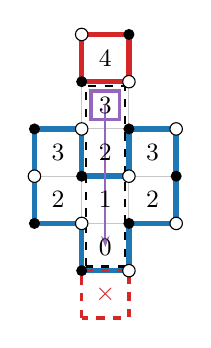
\begin{tikzpicture}[scale=0.6]
\draw[gedge] (0,2) -- (1,2);
\draw[gedge] (0,2) -- (0,3);
\draw[gedge] (0,3) -- (1,3);
\draw[gedge] (0,3) -- (0,4);
\draw[gedge] (0,4) -- (1,4);
\draw[gedge] (1,1) -- (2,1);
\draw[gedge] (1,1) -- (1,2);
\draw[gedge] (1,2) -- (2,2);
\draw[gedge] (1,2) -- (1,3);
\draw[gedge] (1,3) -- (2,3);
\draw[gedge] (1,3) -- (1,4);
\draw[gedge] (1,4) -- (2,4);
\draw[gedge] (1,4) -- (1,5);
\draw[gedge] (1,5) -- (2,5);
\draw[gedge] (1,5) -- (1,6);
\draw[gedge] (1,6) -- (2,6);
\draw[gedge] (2,1) -- (2,2);
\draw[gedge] (2,2) -- (3,2);
\draw[gedge] (2,2) -- (2,3);
\draw[gedge] (2,3) -- (3,3);
\draw[gedge] (2,3) -- (2,4);
\draw[gedge] (2,4) -- (3,4);
\draw[gedge] (2,4) -- (2,5);
\draw[gedge] (2,5) -- (2,6);
\draw[gedge] (3,2) -- (3,3);
\draw[gedge] (3,3) -- (3,4);
\draw[pc1] (0,2) -- (1,2);
\draw[pc1] (0,4) -- (1,4);
\draw[pc1] (1,1) -- (2,1);
\draw[pc1] (1,3) -- (2,3);
\draw[pc1] (2,2) -- (3,2);
\draw[pc1] (2,4) -- (3,4);
\draw[pc1] (0,2) -- (0,3);
\draw[pc1] (0,3) -- (0,4);
\draw[pc1] (1,1) -- (1,2);
\draw[pc1] (1,3) -- (1,4);
\draw[pc1] (2,1) -- (2,2);
\draw[pc1] (2,3) -- (2,4);
\draw[pc1] (3,2) -- (3,3);
\draw[pc1] (3,3) -- (3,4);
\draw[pc2] (1,5) -- (2,5);
\draw[pc2] (1,6) -- (2,6);
\draw[pc2] (1,5) -- (1,6);
\draw[pc2] (2,5) -- (2,6);
\draw[rowbox] (1+0.09,1+0.09) rectangle (1+0.91,4+0.91);
\draw[qbox] (1+0.2,4+0.2) rectangle (1+0.80,4+0.80);
\draw[qarrow] (1+0.5,4+0.5) -- (1+0.5,1+0.5);
\draw[pcB,very thick,dashed] (1,0) rectangle (2,1);
\node[lab,pcB] at (1+0.5,0+0.5) {$\times$};
\node[pt] at (0,2) {};
\node[wpt] at (0,3) {};
\node[pt] at (0,4) {};
\node[pt] at (1,1) {};
\node[wpt] at (1,2) {};
\node[pt] at (1,3) {};
\node[wpt] at (1,4) {};
\node[pt] at (1,5) {};
\node[wpt] at (1,6) {};
\node[wpt] at (2,1) {};
\node[pt] at (2,2) {};
\node[wpt] at (2,3) {};
\node[pt] at (2,4) {};
\node[wpt] at (2,5) {};
\node[pt] at (2,6) {};
\node[wpt] at (3,2) {};
\node[pt] at (3,3) {};
\node[wpt] at (3,4) {};
\node[taulab] at (0+0.5,2+0.5) {$2$};
\node[taulab] at (0+0.5,3+0.5) {$3$};
\node[taulab] at (1+0.5,1+0.5) {$0$};
\node[taulab] at (1+0.5,2+0.5) {$1$};
\node[taulab] at (1+0.5,3+0.5) {$2$};
\node[taulab] at (1+0.5,4+0.5) {$3$};
\node[taulab] at (1+0.5,5+0.5) {$4$};
\node[taulab] at (2+0.5,2+0.5) {$2$};
\node[taulab] at (2+0.5,3+0.5) {$3$};
\end{tikzpicture} & 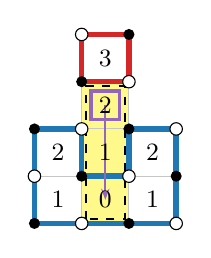
\begin{tikzpicture}[scale=0.6]
\fill[hicell] (1,2) rectangle (2,3);
\fill[hicell] (1,1) rectangle (2,2);
\fill[hicell] (1,0) rectangle (2,1);
\draw[gedge] (0,0) -- (1,0);
\draw[gedge] (0,0) -- (0,1);
\draw[gedge] (0,1) -- (1,1);
\draw[gedge] (0,1) -- (0,2);
\draw[gedge] (0,2) -- (1,2);
\draw[gedge] (1,0) -- (2,0);
\draw[gedge] (1,0) -- (1,1);
\draw[gedge] (1,1) -- (2,1);
\draw[gedge] (1,1) -- (1,2);
\draw[gedge] (1,2) -- (2,2);
\draw[gedge] (1,2) -- (1,3);
\draw[gedge] (1,3) -- (2,3);
\draw[gedge] (1,3) -- (1,4);
\draw[gedge] (1,4) -- (2,4);
\draw[gedge] (2,0) -- (3,0);
\draw[gedge] (2,0) -- (2,1);
\draw[gedge] (2,1) -- (3,1);
\draw[gedge] (2,1) -- (2,2);
\draw[gedge] (2,2) -- (3,2);
\draw[gedge] (2,2) -- (2,3);
\draw[gedge] (2,3) -- (2,4);
\draw[gedge] (3,0) -- (3,1);
\draw[gedge] (3,1) -- (3,2);
\draw[pc1] (0,0) -- (1,0);
\draw[pc1] (0,2) -- (1,2);
\draw[pc1] (1,0) -- (2,0);
\draw[pc1] (1,1) -- (2,1);
\draw[pc1] (2,0) -- (3,0);
\draw[pc1] (2,2) -- (3,2);
\draw[pc1] (0,0) -- (0,1);
\draw[pc1] (0,1) -- (0,2);
\draw[pc1] (1,1) -- (1,2);
\draw[pc1] (2,1) -- (2,2);
\draw[pc1] (3,0) -- (3,1);
\draw[pc1] (3,1) -- (3,2);
\draw[pc2] (1,3) -- (2,3);
\draw[pc2] (1,4) -- (2,4);
\draw[pc2] (1,3) -- (1,4);
\draw[pc2] (2,3) -- (2,4);
\draw[rowbox] (1+0.09,0+0.09) rectangle (1+0.91,2+0.91);
\draw[qbox] (1+0.2,2+0.2) rectangle (1+0.80,2+0.80);
\draw[qarrow] (1+0.5,2+0.5) -- (1+0.5,0+0.5);
\node[pt] at (0,0) {};
\node[wpt] at (0,1) {};
\node[pt] at (0,2) {};
\node[wpt] at (1,0) {};
\node[pt] at (1,1) {};
\node[wpt] at (1,2) {};
\node[pt] at (1,3) {};
\node[wpt] at (1,4) {};
\node[pt] at (2,0) {};
\node[wpt] at (2,1) {};
\node[pt] at (2,2) {};
\node[wpt] at (2,3) {};
\node[pt] at (2,4) {};
\node[wpt] at (3,0) {};
\node[pt] at (3,1) {};
\node[wpt] at (3,2) {};
\node[taulab] at (0+0.5,0+0.5) {$1$};
\node[taulab] at (0+0.5,1+0.5) {$2$};
\node[taulab] at (1+0.5,0+0.5) {$0$};
\node[taulab] at (1+0.5,1+0.5) {$1$};
\node[taulab] at (1+0.5,2+0.5) {$2$};
\node[taulab] at (1+0.5,3+0.5) {$3$};
\node[taulab] at (2+0.5,0+0.5) {$1$};
\node[taulab] at (2+0.5,1+0.5) {$2$};
\end{tikzpicture} \\
\small (a) merge & \small (b) stuck & \small (c) odd row, length $3$
\end{tabular}\\[8pt]
\begin{tabular}{c@{\qquad}c}
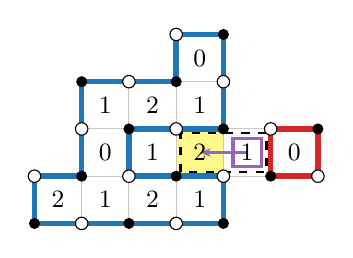
\begin{tikzpicture}[scale=0.6]
\fill[hicell] (3,1) rectangle (4,2);
\draw[gedge] (0,0) -- (1,0);
\draw[gedge] (0,0) -- (0,1);
\draw[gedge] (0,1) -- (1,1);
\draw[gedge] (1,0) -- (2,0);
\draw[gedge] (1,0) -- (1,1);
\draw[gedge] (1,1) -- (2,1);
\draw[gedge] (1,1) -- (1,2);
\draw[gedge] (1,2) -- (2,2);
\draw[gedge] (1,2) -- (1,3);
\draw[gedge] (1,3) -- (2,3);
\draw[gedge] (2,0) -- (3,0);
\draw[gedge] (2,0) -- (2,1);
\draw[gedge] (2,1) -- (3,1);
\draw[gedge] (2,1) -- (2,2);
\draw[gedge] (2,2) -- (3,2);
\draw[gedge] (2,2) -- (2,3);
\draw[gedge] (2,3) -- (3,3);
\draw[gedge] (3,0) -- (4,0);
\draw[gedge] (3,0) -- (3,1);
\draw[gedge] (3,1) -- (4,1);
\draw[gedge] (3,1) -- (3,2);
\draw[gedge] (3,2) -- (4,2);
\draw[gedge] (3,2) -- (3,3);
\draw[gedge] (3,3) -- (4,3);
\draw[gedge] (3,3) -- (3,4);
\draw[gedge] (3,4) -- (4,4);
\draw[gedge] (4,0) -- (4,1);
\draw[gedge] (4,1) -- (5,1);
\draw[gedge] (4,1) -- (4,2);
\draw[gedge] (4,2) -- (5,2);
\draw[gedge] (4,2) -- (4,3);
\draw[gedge] (4,3) -- (4,4);
\draw[gedge] (5,1) -- (6,1);
\draw[gedge] (5,1) -- (5,2);
\draw[gedge] (5,2) -- (6,2);
\draw[gedge] (6,1) -- (6,2);
\draw[pc1] (0,0) -- (1,0);
\draw[pc1] (0,1) -- (1,1);
\draw[pc1] (1,0) -- (2,0);
\draw[pc1] (1,3) -- (2,3);
\draw[pc1] (2,0) -- (3,0);
\draw[pc1] (2,1) -- (3,1);
\draw[pc1] (2,2) -- (3,2);
\draw[pc1] (2,3) -- (3,3);
\draw[pc1] (3,0) -- (4,0);
\draw[pc1] (3,1) -- (4,1);
\draw[pc1] (3,2) -- (4,2);
\draw[pc1] (3,4) -- (4,4);
\draw[pc1] (0,0) -- (0,1);
\draw[pc1] (1,1) -- (1,2);
\draw[pc1] (1,2) -- (1,3);
\draw[pc1] (2,1) -- (2,2);
\draw[pc1] (3,3) -- (3,4);
\draw[pc1] (4,0) -- (4,1);
\draw[pc1] (4,2) -- (4,3);
\draw[pc1] (4,3) -- (4,4);
\draw[pc2] (5,1) -- (6,1);
\draw[pc2] (5,2) -- (6,2);
\draw[pc2] (5,1) -- (5,2);
\draw[pc2] (6,1) -- (6,2);
\draw[rowbox] (3+0.09,1+0.09) rectangle (4+0.91,1+0.91);
\draw[qbox] (4+0.2,1+0.2) rectangle (4+0.80,1+0.80);
\draw[qarrow] (4+0.5,1+0.5) -- (3+0.5,1+0.5);
\node[pt] at (0,0) {};
\node[wpt] at (0,1) {};
\node[wpt] at (1,0) {};
\node[pt] at (1,1) {};
\node[wpt] at (1,2) {};
\node[pt] at (1,3) {};
\node[pt] at (2,0) {};
\node[wpt] at (2,1) {};
\node[pt] at (2,2) {};
\node[wpt] at (2,3) {};
\node[wpt] at (3,0) {};
\node[pt] at (3,1) {};
\node[wpt] at (3,2) {};
\node[pt] at (3,3) {};
\node[wpt] at (3,4) {};
\node[pt] at (4,0) {};
\node[wpt] at (4,1) {};
\node[pt] at (4,2) {};
\node[wpt] at (4,3) {};
\node[pt] at (4,4) {};
\node[pt] at (5,1) {};
\node[wpt] at (5,2) {};
\node[wpt] at (6,1) {};
\node[pt] at (6,2) {};
\node[taulab] at (0+0.5,0+0.5) {$2$};
\node[taulab] at (1+0.5,0+0.5) {$1$};
\node[taulab] at (1+0.5,1+0.5) {$0$};
\node[taulab] at (1+0.5,2+0.5) {$1$};
\node[taulab] at (2+0.5,0+0.5) {$2$};
\node[taulab] at (2+0.5,1+0.5) {$1$};
\node[taulab] at (2+0.5,2+0.5) {$2$};
\node[taulab] at (3+0.5,0+0.5) {$1$};
\node[taulab] at (3+0.5,1+0.5) {$2$};
\node[taulab] at (3+0.5,2+0.5) {$1$};
\node[taulab] at (3+0.5,3+0.5) {$0$};
\node[taulab] at (4+0.5,1+0.5) {$1$};
\node[taulab] at (5+0.5,1+0.5) {$0$};
\end{tikzpicture} & 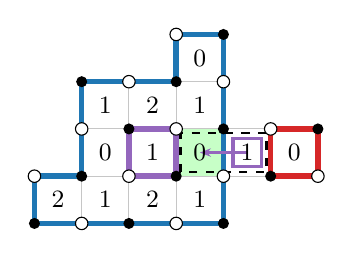
\begin{tikzpicture}[scale=0.6]
\fill[chgcell] (3,1) rectangle (4,2);
\draw[gedge] (0,0) -- (1,0);
\draw[gedge] (0,0) -- (0,1);
\draw[gedge] (0,1) -- (1,1);
\draw[gedge] (1,0) -- (2,0);
\draw[gedge] (1,0) -- (1,1);
\draw[gedge] (1,1) -- (2,1);
\draw[gedge] (1,1) -- (1,2);
\draw[gedge] (1,2) -- (2,2);
\draw[gedge] (1,2) -- (1,3);
\draw[gedge] (1,3) -- (2,3);
\draw[gedge] (2,0) -- (3,0);
\draw[gedge] (2,0) -- (2,1);
\draw[gedge] (2,1) -- (3,1);
\draw[gedge] (2,1) -- (2,2);
\draw[gedge] (2,2) -- (3,2);
\draw[gedge] (2,2) -- (2,3);
\draw[gedge] (2,3) -- (3,3);
\draw[gedge] (3,0) -- (4,0);
\draw[gedge] (3,0) -- (3,1);
\draw[gedge] (3,1) -- (4,1);
\draw[gedge] (3,1) -- (3,2);
\draw[gedge] (3,2) -- (4,2);
\draw[gedge] (3,2) -- (3,3);
\draw[gedge] (3,3) -- (4,3);
\draw[gedge] (3,3) -- (3,4);
\draw[gedge] (3,4) -- (4,4);
\draw[gedge] (4,0) -- (4,1);
\draw[gedge] (4,1) -- (5,1);
\draw[gedge] (4,1) -- (4,2);
\draw[gedge] (4,2) -- (5,2);
\draw[gedge] (4,2) -- (4,3);
\draw[gedge] (4,3) -- (4,4);
\draw[gedge] (5,1) -- (6,1);
\draw[gedge] (5,1) -- (5,2);
\draw[gedge] (5,2) -- (6,2);
\draw[gedge] (6,1) -- (6,2);
\draw[pc1] (0,0) -- (1,0);
\draw[pc1] (0,1) -- (1,1);
\draw[pc1] (1,0) -- (2,0);
\draw[pc1] (1,3) -- (2,3);
\draw[pc1] (2,0) -- (3,0);
\draw[pc1] (2,3) -- (3,3);
\draw[pc1] (3,0) -- (4,0);
\draw[pc1] (3,4) -- (4,4);
\draw[pc1] (0,0) -- (0,1);
\draw[pc1] (1,1) -- (1,2);
\draw[pc1] (1,2) -- (1,3);
\draw[pc1] (3,3) -- (3,4);
\draw[pc1] (4,0) -- (4,1);
\draw[pc1] (4,1) -- (4,2);
\draw[pc1] (4,2) -- (4,3);
\draw[pc1] (4,3) -- (4,4);
\draw[pc4] (2,1) -- (3,1);
\draw[pc4] (2,2) -- (3,2);
\draw[pc4] (2,1) -- (2,2);
\draw[pc4] (3,1) -- (3,2);
\draw[pc2] (5,1) -- (6,1);
\draw[pc2] (5,2) -- (6,2);
\draw[pc2] (5,1) -- (5,2);
\draw[pc2] (6,1) -- (6,2);
\draw[rowbox] (3+0.09,1+0.09) rectangle (4+0.91,1+0.91);
\draw[qbox] (4+0.2,1+0.2) rectangle (4+0.80,1+0.80);
\draw[qarrow] (4+0.5,1+0.5) -- (3+0.5,1+0.5);
\node[pt] at (0,0) {};
\node[wpt] at (0,1) {};
\node[wpt] at (1,0) {};
\node[pt] at (1,1) {};
\node[wpt] at (1,2) {};
\node[pt] at (1,3) {};
\node[pt] at (2,0) {};
\node[wpt] at (2,1) {};
\node[pt] at (2,2) {};
\node[wpt] at (2,3) {};
\node[wpt] at (3,0) {};
\node[pt] at (3,1) {};
\node[wpt] at (3,2) {};
\node[pt] at (3,3) {};
\node[wpt] at (3,4) {};
\node[pt] at (4,0) {};
\node[wpt] at (4,1) {};
\node[pt] at (4,2) {};
\node[wpt] at (4,3) {};
\node[pt] at (4,4) {};
\node[pt] at (5,1) {};
\node[wpt] at (5,2) {};
\node[wpt] at (6,1) {};
\node[pt] at (6,2) {};
\node[taulab] at (0+0.5,0+0.5) {$2$};
\node[taulab] at (1+0.5,0+0.5) {$1$};
\node[taulab] at (1+0.5,1+0.5) {$0$};
\node[taulab] at (1+0.5,2+0.5) {$1$};
\node[taulab] at (2+0.5,0+0.5) {$2$};
\node[taulab] at (2+0.5,1+0.5) {$1$};
\node[taulab] at (2+0.5,2+0.5) {$2$};
\node[taulab] at (3+0.5,0+0.5) {$1$};
\node[taulab] at (3+0.5,1+0.5) {$0$};
\node[taulab] at (3+0.5,2+0.5) {$1$};
\node[taulab] at (3+0.5,3+0.5) {$0$};
\node[taulab] at (4+0.5,1+0.5) {$1$};
\node[taulab] at (5+0.5,1+0.5) {$0$};
\end{tikzpicture} \\
\small (d) bridge step: even row, 2 pieces & \small (e) bridge step: $E$ flipped, 3 pieces
\end{tabular}\\[8pt]
\begin{tabular}{c@{\qquad}c}
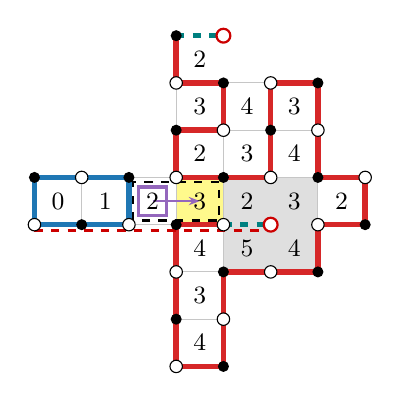
\begin{tikzpicture}[scale=0.6]
\fill[holecell] (4,2) rectangle (5,3);
\fill[holecell] (5,2) rectangle (6,3);
\fill[holecell] (4,3) rectangle (5,4);
\fill[holecell] (5,3) rectangle (6,4);
\fill[hicell] (3,3) rectangle (4,4);
\draw[gedge] (0,3) -- (1,3);
\draw[gedge] (0,3) -- (0,4);
\draw[gedge] (0,4) -- (1,4);
\draw[gedge] (1,3) -- (2,3);
\draw[gedge] (1,3) -- (1,4);
\draw[gedge] (1,4) -- (2,4);
\draw[gedge] (2,3) -- (3,3);
\draw[gedge] (2,3) -- (2,4);
\draw[gedge] (2,4) -- (3,4);
\draw[gedge] (3,0) -- (4,0);
\draw[gedge] (3,0) -- (3,1);
\draw[gedge] (3,1) -- (4,1);
\draw[gedge] (3,1) -- (3,2);
\draw[gedge] (3,2) -- (4,2);
\draw[gedge] (3,2) -- (3,3);
\draw[gedge] (3,3) -- (4,3);
\draw[gedge] (3,3) -- (3,4);
\draw[gedge] (3,4) -- (4,4);
\draw[gedge] (3,4) -- (3,5);
\draw[gedge] (3,5) -- (4,5);
\draw[gedge] (3,5) -- (3,6);
\draw[gedge] (3,6) -- (4,6);
\draw[gedge] (3,6) -- (3,7);
\draw[gedge] (4,0) -- (4,1);
\draw[gedge] (4,1) -- (4,2);
\draw[gedge] (4,2) -- (5,2);
\draw[gedge] (4,2) -- (4,3);
\draw[gedge] (4,3) -- (4,4);
\draw[gedge] (4,4) -- (5,4);
\draw[gedge] (4,4) -- (4,5);
\draw[gedge] (4,5) -- (5,5);
\draw[gedge] (4,5) -- (4,6);
\draw[gedge] (4,6) -- (5,6);
\draw[gedge] (5,2) -- (6,2);
\draw[gedge] (5,4) -- (6,4);
\draw[gedge] (5,4) -- (5,5);
\draw[gedge] (5,5) -- (6,5);
\draw[gedge] (5,5) -- (5,6);
\draw[gedge] (5,6) -- (6,6);
\draw[gedge] (6,2) -- (6,3);
\draw[gedge] (6,3) -- (7,3);
\draw[gedge] (6,3) -- (6,4);
\draw[gedge] (6,4) -- (7,4);
\draw[gedge] (6,4) -- (6,5);
\draw[gedge] (6,5) -- (6,6);
\draw[gedge] (7,3) -- (7,4);
\draw[pc1] (0,3) -- (1,3);
\draw[pc1] (0,4) -- (1,4);
\draw[pc1] (1,3) -- (2,3);
\draw[pc1] (1,4) -- (2,4);
\draw[pc1] (0,3) -- (0,4);
\draw[pc1] (2,3) -- (2,4);
\draw[pc2] (3,0) -- (4,0);
\draw[pc2] (3,3) -- (4,3);
\draw[pc2] (3,4) -- (4,4);
\draw[pc2] (3,5) -- (4,5);
\draw[pc2] (3,6) -- (4,6);
\draw[pc2] (4,2) -- (5,2);
\draw[pc2] (4,4) -- (5,4);
\draw[pc2] (5,2) -- (6,2);
\draw[pc2] (5,6) -- (6,6);
\draw[pc2] (6,3) -- (7,3);
\draw[pc2] (6,4) -- (7,4);
\draw[pc2] (3,0) -- (3,1);
\draw[pc2] (3,1) -- (3,2);
\draw[pc2] (3,2) -- (3,3);
\draw[pc2] (3,4) -- (3,5);
\draw[pc2] (3,6) -- (3,7);
\draw[pc2] (4,0) -- (4,1);
\draw[pc2] (4,1) -- (4,2);
\draw[pc2] (4,5) -- (4,6);
\draw[pc2] (5,4) -- (5,5);
\draw[pc2] (5,5) -- (5,6);
\draw[pc2] (6,2) -- (6,3);
\draw[pc2] (6,4) -- (6,5);
\draw[pc2] (6,5) -- (6,6);
\draw[pc2] (7,3) -- (7,4);
\draw[ph] (4,3) -- (5,3);
\draw[ph] (3,7) -- (4,7);
\draw[slit] (0,3-0.13) -- (5,3-0.13);
\draw[rowbox] (2+0.09,3+0.09) rectangle (3+0.91,3+0.91);
\draw[qbox] (2+0.2,3+0.2) rectangle (2+0.80,3+0.80);
\draw[qarrow] (2+0.5,3+0.5) -- (3+0.5,3+0.5);
\node[wpt] at (0,3) {};
\node[pt] at (0,4) {};
\node[pt] at (1,3) {};
\node[wpt] at (1,4) {};
\node[wpt] at (2,3) {};
\node[pt] at (2,4) {};
\node[wpt] at (3,0) {};
\node[pt] at (3,1) {};
\node[wpt] at (3,2) {};
\node[pt] at (3,3) {};
\node[wpt] at (3,4) {};
\node[pt] at (3,5) {};
\node[wpt] at (3,6) {};
\node[pt] at (3,7) {};
\node[pt] at (4,0) {};
\node[wpt] at (4,1) {};
\node[pt] at (4,2) {};
\node[wpt] at (4,3) {};
\node[pt] at (4,4) {};
\node[wpt] at (4,5) {};
\node[pt] at (4,6) {};
\node[wpt] at (5,2) {};
\node[wpt] at (5,4) {};
\node[pt] at (5,5) {};
\node[wpt] at (5,6) {};
\node[pt] at (6,2) {};
\node[wpt] at (6,3) {};
\node[pt] at (6,4) {};
\node[wpt] at (6,5) {};
\node[pt] at (6,6) {};
\node[pt] at (7,3) {};
\node[wpt] at (7,4) {};
\node[miss] at (4,7) {};
\node[miss] at (5,3) {};
\node[taulab] at (0+0.5,3+0.5) {$0$};
\node[taulab] at (1+0.5,3+0.5) {$1$};
\node[taulab] at (2+0.5,3+0.5) {$2$};
\node[taulab] at (3+0.5,0+0.5) {$4$};
\node[taulab] at (3+0.5,1+0.5) {$3$};
\node[taulab] at (3+0.5,2+0.5) {$4$};
\node[taulab] at (3+0.5,3+0.5) {$3$};
\node[taulab] at (3+0.5,4+0.5) {$2$};
\node[taulab] at (3+0.5,5+0.5) {$3$};
\node[taulab] at (3+0.5,6+0.5) {$2$};
\node[taulab] at (4+0.5,2+0.5) {$5$};
\node[taulab] at (4+0.5,3+0.5) {$2$};
\node[taulab] at (4+0.5,4+0.5) {$3$};
\node[taulab] at (4+0.5,5+0.5) {$4$};
\node[taulab] at (5+0.5,2+0.5) {$4$};
\node[taulab] at (5+0.5,3+0.5) {$3$};
\node[taulab] at (5+0.5,4+0.5) {$4$};
\node[taulab] at (5+0.5,5+0.5) {$3$};
\node[taulab] at (6+0.5,3+0.5) {$2$};
\end{tikzpicture} & 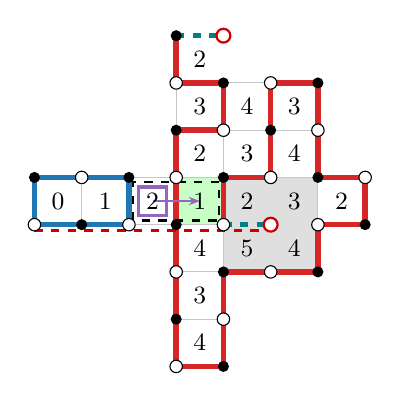
\begin{tikzpicture}[scale=0.6]
\fill[holecell] (4,2) rectangle (5,3);
\fill[holecell] (5,2) rectangle (6,3);
\fill[holecell] (4,3) rectangle (5,4);
\fill[holecell] (5,3) rectangle (6,4);
\fill[chgcell] (3,3) rectangle (4,4);
\draw[gedge] (0,3) -- (1,3);
\draw[gedge] (0,3) -- (0,4);
\draw[gedge] (0,4) -- (1,4);
\draw[gedge] (1,3) -- (2,3);
\draw[gedge] (1,3) -- (1,4);
\draw[gedge] (1,4) -- (2,4);
\draw[gedge] (2,3) -- (3,3);
\draw[gedge] (2,3) -- (2,4);
\draw[gedge] (2,4) -- (3,4);
\draw[gedge] (3,0) -- (4,0);
\draw[gedge] (3,0) -- (3,1);
\draw[gedge] (3,1) -- (4,1);
\draw[gedge] (3,1) -- (3,2);
\draw[gedge] (3,2) -- (4,2);
\draw[gedge] (3,2) -- (3,3);
\draw[gedge] (3,3) -- (4,3);
\draw[gedge] (3,3) -- (3,4);
\draw[gedge] (3,4) -- (4,4);
\draw[gedge] (3,4) -- (3,5);
\draw[gedge] (3,5) -- (4,5);
\draw[gedge] (3,5) -- (3,6);
\draw[gedge] (3,6) -- (4,6);
\draw[gedge] (3,6) -- (3,7);
\draw[gedge] (4,0) -- (4,1);
\draw[gedge] (4,1) -- (4,2);
\draw[gedge] (4,2) -- (5,2);
\draw[gedge] (4,2) -- (4,3);
\draw[gedge] (4,3) -- (4,4);
\draw[gedge] (4,4) -- (5,4);
\draw[gedge] (4,4) -- (4,5);
\draw[gedge] (4,5) -- (5,5);
\draw[gedge] (4,5) -- (4,6);
\draw[gedge] (4,6) -- (5,6);
\draw[gedge] (5,2) -- (6,2);
\draw[gedge] (5,4) -- (6,4);
\draw[gedge] (5,4) -- (5,5);
\draw[gedge] (5,5) -- (6,5);
\draw[gedge] (5,5) -- (5,6);
\draw[gedge] (5,6) -- (6,6);
\draw[gedge] (6,2) -- (6,3);
\draw[gedge] (6,3) -- (7,3);
\draw[gedge] (6,3) -- (6,4);
\draw[gedge] (6,4) -- (7,4);
\draw[gedge] (6,4) -- (6,5);
\draw[gedge] (6,5) -- (6,6);
\draw[gedge] (7,3) -- (7,4);
\draw[pc1] (0,3) -- (1,3);
\draw[pc1] (0,4) -- (1,4);
\draw[pc1] (1,3) -- (2,3);
\draw[pc1] (1,4) -- (2,4);
\draw[pc1] (0,3) -- (0,4);
\draw[pc1] (2,3) -- (2,4);
\draw[pc2] (3,0) -- (4,0);
\draw[pc2] (3,5) -- (4,5);
\draw[pc2] (3,6) -- (4,6);
\draw[pc2] (4,2) -- (5,2);
\draw[pc2] (4,4) -- (5,4);
\draw[pc2] (5,2) -- (6,2);
\draw[pc2] (5,6) -- (6,6);
\draw[pc2] (6,3) -- (7,3);
\draw[pc2] (6,4) -- (7,4);
\draw[pc2] (3,0) -- (3,1);
\draw[pc2] (3,1) -- (3,2);
\draw[pc2] (3,2) -- (3,3);
\draw[pc2] (3,3) -- (3,4);
\draw[pc2] (3,4) -- (3,5);
\draw[pc2] (3,6) -- (3,7);
\draw[pc2] (4,0) -- (4,1);
\draw[pc2] (4,1) -- (4,2);
\draw[pc2] (4,3) -- (4,4);
\draw[pc2] (4,5) -- (4,6);
\draw[pc2] (5,4) -- (5,5);
\draw[pc2] (5,5) -- (5,6);
\draw[pc2] (6,2) -- (6,3);
\draw[pc2] (6,4) -- (6,5);
\draw[pc2] (6,5) -- (6,6);
\draw[pc2] (7,3) -- (7,4);
\draw[ph] (4,3) -- (5,3);
\draw[ph] (3,7) -- (4,7);
\draw[slit] (0,3-0.13) -- (5,3-0.13);
\draw[rowbox] (2+0.09,3+0.09) rectangle (3+0.91,3+0.91);
\draw[qbox] (2+0.2,3+0.2) rectangle (2+0.80,3+0.80);
\draw[qarrow] (2+0.5,3+0.5) -- (3+0.5,3+0.5);
\node[wpt] at (0,3) {};
\node[pt] at (0,4) {};
\node[pt] at (1,3) {};
\node[wpt] at (1,4) {};
\node[wpt] at (2,3) {};
\node[pt] at (2,4) {};
\node[wpt] at (3,0) {};
\node[pt] at (3,1) {};
\node[wpt] at (3,2) {};
\node[pt] at (3,3) {};
\node[wpt] at (3,4) {};
\node[pt] at (3,5) {};
\node[wpt] at (3,6) {};
\node[pt] at (3,7) {};
\node[pt] at (4,0) {};
\node[wpt] at (4,1) {};
\node[pt] at (4,2) {};
\node[wpt] at (4,3) {};
\node[pt] at (4,4) {};
\node[wpt] at (4,5) {};
\node[pt] at (4,6) {};
\node[wpt] at (5,2) {};
\node[wpt] at (5,4) {};
\node[pt] at (5,5) {};
\node[wpt] at (5,6) {};
\node[pt] at (6,2) {};
\node[wpt] at (6,3) {};
\node[pt] at (6,4) {};
\node[wpt] at (6,5) {};
\node[pt] at (6,6) {};
\node[pt] at (7,3) {};
\node[wpt] at (7,4) {};
\node[miss] at (4,7) {};
\node[miss] at (5,3) {};
\node[taulab] at (0+0.5,3+0.5) {$0$};
\node[taulab] at (1+0.5,3+0.5) {$1$};
\node[taulab] at (2+0.5,3+0.5) {$2$};
\node[taulab] at (3+0.5,0+0.5) {$4$};
\node[taulab] at (3+0.5,1+0.5) {$3$};
\node[taulab] at (3+0.5,2+0.5) {$4$};
\node[taulab] at (3+0.5,3+0.5) {$1$};
\node[taulab] at (3+0.5,4+0.5) {$2$};
\node[taulab] at (3+0.5,5+0.5) {$3$};
\node[taulab] at (3+0.5,6+0.5) {$2$};
\node[taulab] at (4+0.5,2+0.5) {$5$};
\node[taulab] at (4+0.5,3+0.5) {$2$};
\node[taulab] at (4+0.5,4+0.5) {$3$};
\node[taulab] at (4+0.5,5+0.5) {$4$};
\node[taulab] at (5+0.5,2+0.5) {$4$};
\node[taulab] at (5+0.5,3+0.5) {$3$};
\node[taulab] at (5+0.5,4+0.5) {$4$};
\node[taulab] at (5+0.5,5+0.5) {$3$};
\node[taulab] at (6+0.5,3+0.5) {$2$};
\end{tikzpicture} \\
\small (f) twist: even row, 2 pieces & \small (g) twist: $E$ flipped, still 2 pieces
\end{tabular}\\[10pt]
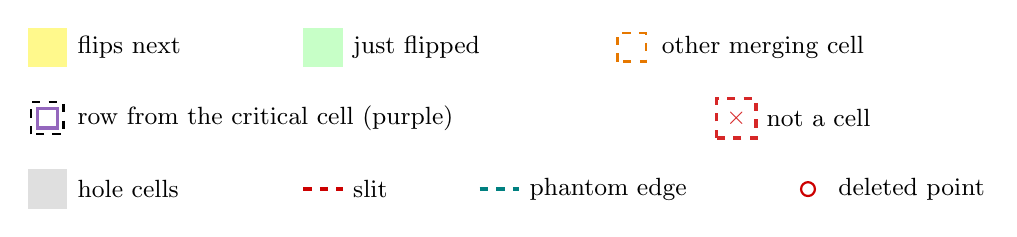
\begin{tikzpicture}[scale=0.5]
\fill[hicell] (0.0,0.0) rectangle (1.0,1.0);
\node[lab,anchor=west] at (1.15,0.5) {flips next};
\fill[chgcell] (7.000000000000001,0.0) rectangle (8.0,1.0);
\node[lab,anchor=west] at (8.15,0.5) {just flipped};
\draw[candbox] (14.980000000000002,0.14) rectangle (15.700000000000001,0.86);
\node[lab,anchor=west] at (15.990000000000002,0.5) {other merging cell};
\draw[rowbox] (0.09,-1.71) rectangle (0.91,-0.89);\draw[qbox] (0.25,-1.55) rectangle (0.75,-1.05);
\node[lab,anchor=west] at (1.15,-1.3) {row from the critical cell (purple)};
\draw[pcB,very thick,dashed] (17.5,-1.8) rectangle (18.5,-0.8);\node[lab,pcB] at (18.0,-1.3) {$\times$};
\node[lab,anchor=west] at (18.65,-1.3) {not a cell};
\fill[holecell] (0.0,-3.6) rectangle (1.0,-2.6);
\node[lab,anchor=west] at (1.15,-3.1) {hole cells};
\draw[slit] (7.000000000000001,-3.1) -- (8.0,-3.1);
\node[lab,anchor=west] at (8.15,-3.1) {slit};
\draw[ph] (11.48,-3.1) -- (12.48,-3.1);
\node[lab,anchor=west] at (12.63,-3.1) {phantom edge};
\node[miss] at (19.82,-3.1) {};
\node[lab,anchor=west] at (20.47,-3.1) {deleted point};
\end{tikzpicture}

\caption{The outcomes of one phase step, with a height in every cell.
The arrow in a row points in its direction.
(a) Merge.
The yellow cell is a merging cell, alternating with its corners in two pieces, and the first in
the scan order.
(b) Stuck.
There is no merging cell, and the row of the only critical cell falls $3,2,1,0$ into a square that
is not a cell (red cross) before its heights turn.
(c) Odd.
There is no merging cell, and the row of the critical cell has odd length $3$.
Lowering it joins the two pieces.
(d), (e) Bridge step.
The row has even length $2$, and flipping its last cell $E$ splits the blue piece in two.
The phase records the bridge and continues.
(f), (g) Twist.
A path factor of a leaf with an inner endpoint, whose phantom lies in the hole (grey cells, slit
heights, slit dashed red).
The row has even length $2$, and flipping its last cell $E$ splits nothing, because the strand
through $E$ belongs to the path piece.
The phase ends and lowers the whole row, which joins the two pieces.}
\label{fig:phase}
\end{figure}

\subsection{Success branches and the undoing of bridges}
\label{sec:undo}

The outcomes merge, odd and twist each give a \emph{half bridge}.
The half bridge is a flip of a merging cell, the lowering of an odd row, or the lowering of an
even row.
Lowering a row flips its cells from the last down to the first.
We follow Sheffield in calling this lowering.
Along a rising row it lowers every height of the row by $2$, and along a falling row it raises every
height by $2$, by symmetry.
Each of these operations joins one pair of pieces.
The bridges are then processed in reverse order of creation.
The \emph{pending pair} is first the pair of points whose pieces the half bridge joins.
Bridge $i$ is \emph{lowered} (its row without $E_i$ is flipped) when the pending pair is connected
in the state before bridge $i$, and its start pair $(b_1,f_1)$ of $q_i$ becomes the pending pair.
Otherwise it is \emph{undone} ($E_i$ is flipped back).
This rule is computable (Lean \lean{plan}, \lean{planB}).
It reproduces Sheffield's path in his boundary tree without building the tree.

\begin{theorem}[undoing the bridges, \lean{undo\_count}, \lean{UndoCount.lean}]
\label{thm:undo}
If the operations of the plan are compatible, then applying the half bridge and the plan to the
final state of the phase gives a bridge-free factor with $m-1$ pieces.
\end{theorem}

\emph{Compatible} (\lean{OpsOK}) means two things.
Each operation is an intact odd strip of cells, its end pair lies in a fixed set $P$ of points, and
no point of $P$ is an interior point of the strip.
No edge toggled by an earlier operation is a side of a cell of a later one.
This is Sheffield's Lemma~4.

\begin{proof}[Proof sketch]
The half bridge joins the pieces of a pending pair $(u,v)$ (\lean{join\_apply}).
The proof is an induction over the bridges, newest first, with this invariant.
The current factor $G$ has one piece fewer than the state $H$ with the remaining bridges, the
connections of $G$ on $P$ are those of $H$ with $u$ and $v$ joined, and $u,v$ are apart in $H$.
Going back over a bridge $b$ removes one piece from $H$ (\lean{step\_count}).
If $u$ and $v$ are joined in the state before $b$, the plan lowers the row of $b$ without $E$.
That is an odd strip whose start pair is apart in $G$, because the critical cell $b.q$ has its back
and front corners in different pieces.
If $u$ and $v$ are not joined there, the plan flips $E$ back, and the back and front corners of $E$
are apart in $G$, because the bridge step split them (\lean{RowStep.split}).
In both cases, flipping an intact odd strip whose end pair is apart removes one piece and joins
that pair (\lean{strip\_odd\_pf}), so the invariant holds for the earlier state, with the start pair
of $b$ as the new pending pair after a lowering (\lean{merge\_eq\_prev}).
Compatibility keeps the later strips intact (\lean{OpsOK.tail}).
With no bridges left the gap of one piece gives $m-1$ pieces.
\end{proof}

Compatibility is proved in Lean for every operation pair (\lean{opsOK\_rows},
\lean{opsOK\_merge}).
The regions of the bridges keep their edge pattern through later steps (\lean{regionOK\_step}), and
the square flipped by one bridge lies outside the region of every other.
From these, the half bridge toggles no side of a square of the plan (\lean{c2\_chain},
\lean{c2\_merge}), its cells avoid the bridge squares (\lean{c1\_half}, \lean{c1\_merge}), the
squares of different operations are disjoint (\lean{c1\_newer}), and an earlier operation toggles no
side of a later one (\lean{c2\_plan}).
Each of these is a case analysis on which side of which square a toggled edge lies, with the cases
named \lean{caseA1}, \lean{caseA2}, \lean{caseB2}, \lean{caseB3} and \lean{caseB4} in Lean.
Only \lean{caseA2}, an out-vertex at the front of a bridge end, uses Far.
One configuration of the merge branch, two bridge ends crossed at one merging cell, is not
excluded.
It is avoided by a choice rule.
A merging cell $X$ is \emph{good} when no bridge $i$ that the plan started from $X$ undoes ends at
$X$, that is, has $X$ as the square beyond $E_i$.
\begin{theorem}[Theorem~R, \lean{theoremR}, \lean{S4TheoremR.lean}]
\label{thm:R}
Let the phase start from a factor whose out-vertices $t_0,u_0$ are Far and carry no opposed
phantoms (\lean{NoOpp}, \cref{def:far,def:opp}).
In the merge outcome a good merging cell exists.
\end{theorem}

\begin{proof}[Proof sketch]
Suppose every merging cell is bad, and let $X$ be bad through an undone bridge $i$, so $X$ is the
square beyond $E_i$.
In the frame of $E_i$, $X$ has dark back and front and light laterals (\lean{beyond\_facts}).
Each square beside $E_i$ across a lateral is a cell, or a corner of $E_i$ on that side is an
out-vertex whose phantom lies across that lateral (\lean{side\_or\_t}).
A side square that is a cell is a merging cell (\lean{l22}), so it is bad through some undone bridge
$k$.
Then the two bridges are crossed.
The front of $E_k$ faces opposite to the front of $E_i$, $E_k$ is the square beside $X$, and $k$ is
determined by $X$ alone, as the bridge Lean calls the node of $X$ (\lean{l23}).
If both side squares are cells, both give this same $k$, and $E_k$ would be two different
squares.
If one is a cell and the other holds an out-vertex, the square beside $E_k$ on its far side is a
cell, since otherwise a second out-vertex would carry a phantom opposed to the first, which
\lean{NoOpp} excludes (\lean{t\_farA2}, \lean{t\_farB2}).
That cell is merging and bad through some $k'$, and the node facts force $k'=i$ and a geometric
contradiction (\lean{r\_core}, \lean{node\_beside}).
If both sides hold out-vertices, two out-vertices are corners of one cell, which contradicts Far
(\lean{two\_sides}).
\end{proof}
The algorithm takes the first cell passing the computable test \lean{goodB}.
It is computed as \lean{isGoodMergingCell}, which builds the connections of each intermediate state
once (\lean{isGoodMergingCell\_eq}).

\subsection{The certificate}

\begin{definition}[certificate, \lean{Cert}, \lean{Cert.lean}]
\label{def:cert}
Let $H$ be a factor, $\mathrm{FP}$ a list of fixed pairs, and $t_0,u_0$ points (the out-vertices,
\cref{def:far}).
$\lean{Cert}\ V\ H\ \mathrm{FP}\ t_0\ u_0$ is the conjunction of the following local conditions.
\begin{enumerate}[label=(\arabic*)]
\item Every merging cell is a pair square of a pair in $\mathrm{FP}$ (\lean{f2}).
\item Every pair satisfies \lean{PairOK}.
  A pair has a top square and a bottom square (Lean \lean{top}, \lean{bot}).
  The light sides of the top square have arcs pointing in, those of the bottom square point out,
  the arc across their shared side points from the bottom square to the top square, and the pieces
  at the corners of both squares are recorded.
\item Every cell touching three or more pieces has the E1 shape at $t_0$ or $u_0$ or the diagonal
  shape (\lean{TriOK}).
\item Every edge with one end outside $V$ has its other end at $t_0$ or $u_0$ (\lean{out}).
\item No cell with joined back corners, joined front corners and different back and front pieces
  has both back and front light (\lean{l4}).
\item Pair squares are alternating, the shared side of a pair is dark, and pairs are disjoint.
\item For every critical cell with dark back that is not a pair square, its \emph{chained row}
  (\cref{sec:repair}) ends at a pair square of its direction, or it leaves $V$ with all its arcs
  pointing one way (\lean{col}).
\item The same holds for strips that start beside the square just beyond a pair (\lean{side}).
\end{enumerate}
\end{definition}

\lean{Cert} mentions only $V$, $H$, $\mathrm{FP}$, $t_0$ and $u_0$.
It does not mention any competitor factor.

\begin{theorem}[\lean{cert\_count\_gen}]
\label{thm:cert}
Let $H$ and $H'$ be factors of $W\supseteq V$ with the same degrees, agreeing off the edges of $V$.
Assume every corner of a cell of $V$ has degree $2$, $\lean{SolidFor}\ V\ H\ H'$ holds, and no
factor of $W$ with these degrees has a closed climb (\lean{ClimbAcyc}, \cref{def:climb}).
If $\lean{Cert}\ V\ H\ \mathrm{FP}\ t_0\ u_0$ holds, then
$\ncomp(W,H)\le\ncomp(W,H')+|\mathrm{FP}|$.
\end{theorem}

\begin{proof}
\lean{Cert} implies the invariant \lean{Inv} for the competitor $H'$ (\lean{cert\_inv}), and
\cref{thm:minimal} gives the bound.
The only difference between the two is in fields (7) and (8).
\lean{Cert} allows a chained row to leave $V$ with all its arcs pointing one way, and \lean{Inv}
requires it to end at a pair square.
A chained row that leaves $V$ cannot carry $D(H,H')$ of its direction's sign, because $D$ does not
move back toward $0$ along arcs and is $0$ off the cells (\lean{not\_colOut}).
\end{proof}

\begin{theorem}[\lean{cert\_of\_stuck}, \lean{TriProof.lean}]
\label{thm:stuckcert}
Let the phase start from a factor whose edges leaving $V$ all end at $t_0$ or $u_0$, and let
$t_0,u_0$ be Far (\cref{def:far}).
If the phase ends with outcome stuck in state $H$ with bridge list $\mathrm{BS}$, then
$\lean{Cert}\ V\ H\ (\mathrm{BS}.\mathrm{map}\ \lean{pairOf})\ t_0\ u_0$ holds.
\end{theorem}

\begin{proof}[Proof sketch]
Along the bridge steps of the phase an invariant holds (\lean{pinv\_reach}).
The state is a factor, its edges leaving $V$ end at $t_0$ or $u_0$, the region of every bridge keeps
its edge pattern (\lean{regionOK\_new}, \lean{regionOK\_step}), the pair squares of different bridges
are distinct, and the square flipped by one bridge lies outside the region of every other.
At the stuck state, every merging cell is a pair square by the stopping rule.
The fields of \lean{Cert} follow (\lean{cert\_of\_phase}).
Field~(1) is the stopping rule.
Fields~(2) and~(6) come from the frozen regions of the bridges (\lean{pair\_facts}).
Field~(4) is part of the invariant.
Fields~(3) and~(5) come from degree~$2$ at the corners.
A cell that violates them forces a square across one of its sides to be a non-cell with an
out-vertex at a corner of the cell (\lean{across\_noncell}), and a violation on two sides would put
two different out-vertices at corners of one cell, which contradicts Far (\lean{tri\_of},
\lean{l4\_of}).
Fields~(7) and~(8) come from the rule that no critical cell is left unstuck, through the chaining
lemma below (\lean{col\_of\_stuck}, \lean{side\_of\_stuck}).
\end{proof}

A stuck state has $m+\ell$ pieces with $\ell=|\mathrm{BS}|$.
If a Hamiltonian path exists, \cref{thm:cert} with $H'$ the path gives $m+\ell\le 1+\ell$.
So $m\le1$, and when a Hamiltonian path exists a phase from $m\ge2$ pieces never ends stuck.
The ``no'' answer is therefore certified by a local check.
It does not depend on the phase rules.
The phase rules are needed only for completeness, that is, for showing that a phase ends in a
merge or in a certified state.

\subsection{Chained rows and the stuck case}
\label{sec:repair}

The count behind \cref{thm:cert} compares a stuck state $H$ with a competitor $H'$.
Generalized moves along chained rows bring $H$ toward $H'$ without changing the number of pieces or
of fixed pairs, and the joins between pieces that remain are then counted.
In Sheffield's \S4.5, as in \cref{def:row}, a row stops where its front arc turns, and a critical
cell is stuck when its row first reaches a square that is not a cell or is a cut cell.
Rows run in all four directions.
His move in \S4.8 lowers rows that end at a fixed pair.
A stuck row can instead end at a cut cell $g$.
Then the run continues straight through $g$, possibly through further cut cells, until it reaches
a fixed pair or leaves $V$ (\cref{lem:chain}).
The whole straight run is a \emph{chained row}.
It differs from a row not in direction but in passing through cut cells.
Lowering it reroutes strands at those cut cells without joining pieces there, and
\cref{app:repair} shows that Sheffield's count reads this rerouting as joining.

\begin{definition}[strip, chained row]
A \emph{strip} of length $n$ from $c$ is a straight run $c_0,\dots,c_{n-1}$ with dark back of $c_0$,
laterals of $c_j$ dark exactly for odd $j$, and the front of $c_j$ dark exactly for odd $j$, except
that the last front is dark exactly when $n$ is odd (Lean \lean{StripPat}).
A \emph{chained row} from a critical cell $c$ is a strip $c_0=c,\dots,c_n$ that ends in one of two
ways.
Either its last cell $c_n$ and the square $c_{n+1}$ beyond it form a fixed pair (Lean
\lean{ColEnds}), or it leaves $V$ with all its arcs pointing one way (Lean \lean{ColOut}).
Its length is $n+1$, the length of the strip, and the Lean files call it a column.
\end{definition}

\begin{lemma}[chaining lemma, \lean{col\_of\_stuck}, \lean{lemmaC}, \lean{ColProof.lean}]
\label{lem:chain}
Let $q$ be critical with dark back, and let its row be stuck at a cut cell $g=c_k$.
Then $k$ is even, $g$ has a dark back and light laterals, and one of the following holds.
\begin{enumerate}
\item The front of $g$ is dark, and $g$ is a pair square with its partner in front.
\item The front of $g$ is light, its front corners are joined, and $g$ is critical in the same
  frame and direction, so the run continues with the row of $g$.
\item The front of $g$ is light, its front corners are apart, and the square in front of $g$ is not
  a cell of $V$.
\end{enumerate}
\end{lemma}

\begin{proof}[Proof sketch]
Along the row the arcs all point the same way, so its cells have the strip pattern, with laterals
and front of $c_j$ dark exactly for odd $j$ (\lean{run\_pat}).
If $k$ were odd, the front of $c_{k-1}$ and its laterals would be light, degree~$2$ would darken the
laterals of $g$, and $g$ would not be cut (\lean{uncut\_of}).
So $k$ is even, the shared side is dark, and degree~$2$ makes the laterals of $g$ light
(\lean{forcedA'}, \lean{forcedB'}).
If the front of $g$ is dark, $g$ is alternating and cut, so it is a merging cell and, at a stuck
state, a pair square.
If the front is light and its corners are joined, $g$ is critical with the same front arc
(\lean{arc\_opp\_diff}), and the argument repeats along the row of $g$ (\lean{lemmaC}).
If the front corners are apart, a merging-cell argument shows that the square in front is not a
cell.
The strips glue into one strip (\lean{stripPat\_append}).
\end{proof}

\begin{lemma}[strand pairing, \lean{lowerCol\_count}, \lean{Column.lean}]
\label{lem:strand}
Lowering a chained row toggles all its laterals and its two end sides.
It keeps the pairing of the strands that leave it sideways at the odd positions $j$ along it.
Only the strands at its two ends can change partners.
So a chained row changes the number of pieces exactly as one row of the same length.
\end{lemma}

The proof of \cref{lem:strand} is in \cref{app:strand}.

The proof uses chained rows in place of rows in the move.
Say that $D(H,H')$ has \emph{sign} $o$ at a cell when it is positive for $o=\lean{true}$ and negative
for $o=\lean{false}$ (Lean \lean{sgnD}), and write $o$ for the front arc of a critical cell, true when
it points out.
A \emph{generalized move} at a critical cell $c$ with $D$ of sign $o$ lowers the chained row from
$c_1$ to its last cell and makes $(c_0,c_1)$ the new fixed pair.
It keeps the number of pieces (\cref{lem:strand}), keeps the invariant \lean{Inv}
(\lean{MoveInv.lean}, \lean{ColAfter.lean}, \lean{SideAfter.lean}, \lean{E1After.lean}), and lowers
$\mu=\sum_c|D(H,H')(c)|$ by $2$ for each flipped cell.
The square beyond a pair created by a move need not be a cut cell, and the invariant has a field
\lean{side} for it.
The E1 square is handled by a shape invariant instead of a count.

\begin{theorem}[\lean{stuck\_minimal}, \lean{Minimal.lean}]
\label{thm:minimal}
If $\lean{Inv}\ V\ H\ H'\ \mathrm{FP}\ t_0\ u_0$ holds, then
$\ncomp(W,H)\le\ncomp(W,H')+|\mathrm{FP}|$.
\end{theorem}

\begin{proof}[Proof sketch]
The proof is an induction on $\mu$.

\emph{A move exists.}
Suppose some cell $c$ with joined back corners, joined front corners and different back and front
pieces is not alternating and has $D(H,H')$ of sign $o$.
By field~(5) and degree~$2$, $c$ is critical in a frame with dark back and front arc $o$
(\lean{crit\_of\_twotwo}), and it is not a pair square (\lean{not\_pair\_of\_crit}).
Field~(7) gives a chained row $c_0=c,\dots,c_n$ whose last cell and the square $c_{n+1}$ beyond it
form a pair $i$, with $n$ even and $n\ge2$ (\lean{movable\_column}).
The move flips $c_n,\dots,c_1$ and replaces the pair $i$ by the pair $(c_0,c_1)$, so the number of
pairs is unchanged (\lean{fpAfter\_length}).
The flips keep the factor, its number of pieces and its connections away from the inner corners of
the chained row (\lean{lowerCol\_factor}).
They keep \lean{Inv}, with \lean{col\_after} for field~(7), \lean{sideInv\_after} for field~(8),
\lean{three\_after} for field~(3) and \lean{MoveCtx.out\_after} for field~(4) (\lean{MoveCtx.inv\_after}).
Each flipped cell is a local extremum with $D$ of the right sign, so $\mu$ drops by $2n\ge4$
(\lean{lowerCol\_mu}, \lean{MoveCtx.mu\_lt}), and the induction hypothesis applies.

\emph{No move exists.}
Call a cell $c$ \emph{extremal} along the cut between two pieces $Q_1\ne Q_2$ of $H$ in direction
$o$ when no side of $c$ with one end in $Q_1$ and the other in $Q_2$ has its arc pointing in
direction $o$.
Say that a pair \emph{pays} for the cut $Q_1|Q_2$ when the corner pieces recorded in field~(2) are
$Q_1$ and $Q_2$ and $D(H,H')$ has the matching sign at its square.
Then every cell $c$ that is extremal along a cut $Q_1|Q_2$, with $D(H,H')(c)\neq0$ of the matching
sign, is a square of a pair that pays for $Q_1|Q_2$, or it is the E1 square and the cut is paid
through a third piece $Q_3$ (\lean{finalOK\_of}, \lean{threeOK\_of\_tri}).
Let $P$ be the paying pairs, so $|P|\le|\mathrm{FP}|$.
Take an edge $e$ of $H'$ that joins two pieces of $H$.
Beside $e$ lies a square with $D\neq0$ (\lean{disagree\_beside}), which is a cell by
\lean{SolidFor}.
A climb from it along the cut never decreases $|D|$ and ends, because no climb closes, at an
extremal cell (\lean{climb}).
The paying pair there joins the two ends of $e$ in the pieces of $H$ merged along $P$.
So every edge of $H'$ that joins pieces of $H$ is accounted for by $P$, and the rank bound
(\lean{ncomp\_le\_of\_joins}, \lean{final\_count}) gives $\ncomp(W,H)\le\ncomp(W,H')+|P|$.
\end{proof}

\subsection{Climbs}

\begin{definition}[climb]
\label{def:climb}
A \emph{climb step} in direction $o$ goes from a cell $c$ to a neighbouring cell $c'$ across a
side whose arc points from $c$ to $c'$ (for $o=\lean{true}$) or from $c'$ to $c$ (for
$o=\lean{false}$), and whose two ends lie in two given pieces $x\ne y$ (Lean \lean{ClimbStep}).
\lean{ClimbAcyc} says that no sequence of climb steps returns to its start.
\lean{ArcAcyc} is the same condition without the piece restriction (\lean{SlitHeight.lean}).
\end{definition}

The final count follows a climb from a cell with $D\ne0$ along its cut to an extremal cell
(\lean{climb}, \lean{Final.lean}).
With a height the climb ends because $\tau$ rises (\lean{acyc\_of\_height}).
The Lean proof of \lean{climb} uses only \lean{ClimbAcyc}.
Its measure is the number of cells reachable by climb steps.

\subsection{The loop}
\label{sec:loop}

The loop \lean{runSC} starts from any path factor.
It repeats phases, and each successful phase is followed by the reduction of \cref{thm:undo}.
Each round removes one piece.
The loop answers \lean{true} when one piece remains and \lean{false} on a stuck phase.
Its fuel is $|V|+2$ rounds, and each phase has fuel $|W|+1$ bridge steps.

The algorithms use a fast version of the two-phantom loop, \lean{twoPhantomLoop}, with the same answers.
\begin{itemize}
\item \lean{connectedPairs}~$W\ H$ lists all connected pairs of points in one sweep, computing each
  component once, in $O(|W|^2)$ steps (\lean{connectedPairsCost\_le}, \lean{isConnected\_eq},
  \lean{ConnSet.lean}).
\item The phase \lean{runPhase} computes the connection set once per step, together with the set of
  bridge cells, so each step costs $O(|W|^2)$.
  It equals \lean{phase} on the states the phase reaches (\lean{runPhase\_eq}, \lean{PhaseS.lean}).
\item The reduction \lean{reducePieces} computes the connection sets of the bridge states once, and
  the plan of each candidate merging cell once, in $O(|W|^3)$ steps (\lean{reducePieces\_eq},
  \lean{ReduceS.lean}).
\item The fast loop \lean{twoPhantomLoop} equals \lean{runSC2}, the loop \lean{runSC} for
  two-phantom factors (\lean{twoPhantomLoop\_eq}).
  With fuel $n$ it costs at most $(n+1)\cdot 3000\,(|V|+3)^3$ (\lean{twoPhantomLoopCost\_le},
  \lean{LoopF.lean}).
\end{itemize}

% =====================================================================
\section{Phantom endpoints and the two-phantom core}
\label{sec:phantom}

Sheffield's argument needs degree $2$ at every corner of a flipped cell.
A path endpoint has degree $1$.
The fix is to move the degree-one defect of each endpoint off $V$.

\begin{definition}[phantom]
Let $t\in V$ have a missing lattice neighbour $p$.
A \emph{phantom factor} is a factor on $V\cup\{p\}$ with degrees $d_{sp}$ that contains the edge
$t$--$p$ and no other edge at $p$ (Lean \lean{NotchF}, \lean{NotchPF.lean}).
The point $p$ is the \emph{phantom} of $t$, and $t$--$p$ is the \emph{phantom edge}.
\end{definition}

In a phantom factor $t$ has degree $2$ and the endpoint is $p\notin V$.
Phantom factors correspond one to one to path factors of $V$ (\lean{notch\_up},
\lean{notch\_down}), with the same pieces.
Only cells of $V$ are flipped, so $p$ is never the corner of a flipped cell.

\begin{definition}[two phantoms]
Let $t$ and $s$ have missing lattice neighbours $p\ne q$.
A \emph{two-phantom factor} is a factor on $V\cup\{p,q\}$ with degree $1$ at $p$ and $q$ and $2$ on
$V$, containing $t$--$p$ and $s$--$q$ and no other edge at $p$ or $q$ (Lean \lean{NotchF2},
\lean{TwoPh.lean}).
\end{definition}

\begin{definition}[out-vertex, Far]
\label{def:far}
An \emph{out-vertex} of a factor is a point of $V$ joined by an edge of the factor to a point
outside $V$.
In a two-phantom factor the out-vertices are $t$ and $s$ (\lean{two\_out}).
Two points $t_0,u_0$ are \emph{Far} when $t_0=u_0$ or $\dist(t_0,u_0)\ge2$ (Lean \lean{Far},
\lean{Close1}, \lean{StuckL4.lean}).
\end{definition}

\begin{definition}[opposed phantoms]
\label{def:opp}
Let $a,b$ be out-vertices with phantoms $m_a,m_b$.
The phantoms are \emph{opposed} when $a$ and $b$ differ by exactly $2$ along one axis and by at
most $2$ along the other, and $m_a$ and $m_b$ point away from each other along the first axis
(Lean \lean{Opp}).
For example $a=(0,0)$, $m_a=(-1,0)$, $b=(2,1)$, $m_b=(3,1)$ are opposed.
\lean{NoOpp}~$V\ H\ t_0\ u_0$ says that no two distinct out-vertices of $H$ carry opposed phantoms.
For a two-phantom factor, $\lean{FarN}\ t\ p\ s\ q$ means that $t,s$ are Far and the phantoms $p$ of
$t$ and $q$ of $s$ are not opposed (\lean{TwoPh.lean}).
\lean{FarN} gives \lean{NoOpp} for every two-phantom factor (\lean{two\_noOpp}).
\end{definition}

Several sites of the certificate argument concern the out-vertex (\lean{l4\_of}, \lean{tri\_of},
\lean{a2p}, \lean{side\_or\_t}, \lean{t\_farA}, and others).
With two out-vertices every site but two closes under Far, because two different corners of one cell lie within king
distance $1$ (\lean{two\_sides}, \lean{corners\_close}).
Two sites need more, \lean{t\_farA2} and \lean{t\_farB2} in the proof of Theorem~R (the crossed
configuration in the proof of \cref{thm:R}).
There one out-vertex sits at a corner of the bridge end $E$ and the other at a corner of a cell two
steps away, at king distance $2$ in the worst case.
Both sites close by \lean{NoOpp}, using the phantom positions returned by \lean{side\_or\_t}.
So \lean{theoremR} takes the hypotheses Far and \lean{NoOpp} for the start factor of the phase.

\begin{theorem}[\lean{hpSheffC2\_main}, \lean{TwoPhCost.lean}]
\label{thm:twoph}
Let $V$ be solid, and let $s\ne t$ in $V$ have missing lattice neighbours $q\ne p$ with
$\lean{FarN}\ t\ p\ s\ q$.
Then \lean{hpSheffC2} decides whether $V$ has a Hamiltonian $s$--$t$ path
(\lean{hpSheffC2\_main}).
Its fast version \lean{twoPhantomTest} returns the same answer (\lean{twoPhantomTest\_eq}) within
$5000(|V|+3)^4$ steps (\lean{twoPhantomTestCost\_le}, \lean{LoopF.lean}).
\end{theorem}

\begin{proof}
Applied at both endpoints, the correspondence of phantom factors with path factors
(\lean{notch\_up}, \lean{notch\_down}) shows that $V$ has a Hamiltonian $s$--$t$ path exactly when
some two-phantom factor on $W=V\cup\{p,q\}$ has one piece.
If \lean{findFactor} finds no path factor, none exists (\lean{findFactor\_none}) and the answer
\lean{false} is correct.
Otherwise the loop runs on two-phantom factors, and the hypotheses of \cref{sec:sheffield} hold for
any two of them, $H$ and $H'$.
Every corner of a cell of $V$ has degree $2$, because the degree-one points $p$ and $q$ are outside
$V$.
$H\oplus H'$ consists of edges of $V$, because both contain $t$--$p$ and $s$--$q$ and no other edge
at $p$ or $q$, so \cref{lem:D} gives $\lean{SolidFor}\ V\ H\ H'$.
Every two-phantom factor has a height by \cref{lem:height}, and a height rises along every climb,
so no climb closes (\lean{acyc\_of\_height}).
The out-vertices $t$ and $s$ are Far with phantoms that are not opposed (\lean{two\_noOpp}).
Suppose a phase starts with $m$ pieces.
If it ends stuck after $\ell$ bridge steps, its state has $m+\ell$ pieces and satisfies the
certificate with $\ell$ fixed pairs (\cref{thm:stuckcert}), so every two-phantom factor has at least $m$ pieces
(\cref{thm:cert}).
A phase is only run while $m\ge2$, so then no Hamiltonian path exists and \lean{false} is correct.
Otherwise the phase ends with a merge, an odd row or a twist.
\Cref{thm:R} supplies a good merging cell in the merge case, and \cref{thm:undo} turns the outcome
into a bridge-free factor with $m-1$ pieces.
A phase cannot run out of fuel, since each bridge step adds a piece and there are at most $|W|$
pieces.
So each round removes one piece, and the $|V|+2$ rounds of fuel reach one piece, where the answer
\lean{true} is correct.
The fast loop computes the same rounds (\lean{twoPhantomLoop\_eq}).
Each round costs at most $3000(|V|+3)^3$, and with $|V|+2$ rounds and \lean{findFactor} the total is
within $5000(|V|+3)^4$.
\end{proof}

% =====================================================================
\section{Deletion walks}
\label{sec:walk}

\begin{lemma}[deletion, \lean{del\_iff}, \lean{TwoPhWalk.lean}]
\label{lem:del}
Let $s\ne t$ be in $V$ with $|V|\ge3$.
Then $V$ has a Hamiltonian $s$--$t$ path if and only if, for some lattice neighbour $w\ne s$ of
$t$ in $V$, the set $V\setminus\{t\}$ has a Hamiltonian $s$--$w$ path.
\end{lemma}

\begin{proof}
Let $H$ be a Hamiltonian $s$--$t$ path of $V$.
The point $t$ has degree $1$, so exactly one edge $w$--$t$ of $H$ meets $t$.
Since $|V|\ge3$, the path is not the single edge $s$--$t$, so $w\ne s$.
Removing this edge gives a Hamiltonian $s$--$w$ path of $V\setminus\{t\}$.
Conversely, adding the edge $w$--$t$ to a Hamiltonian $s$--$w$ path of $V\setminus\{t\}$ gives a
Hamiltonian $s$--$t$ path of $V$.
\end{proof}

The deleted point $t$ is a missing lattice neighbour of $w$, so it can serve as the phantom of $w$.
If $t$ has a missing king neighbour, $V\setminus\{t\}$ is solid (\lean{solid\_erase}).

\paragraph{The walk.}
The walk \lean{boundaryEndpointsWalk} keeps $s$ with its phantom fixed and moves $t$.
In state $(V,t)$ it does the following.
A \emph{usable phantom} of $t$ is a missing lattice neighbour of $t$ that differs from the phantom
$q$ of $s$ and is not opposed to $q$ (Lean \lean{isUsablePhantom}).
If $t$ has a usable phantom and $t,s$ are Far, the walk runs \lean{twoPhantomTest} with the first usable phantom.
Otherwise it deletes $t$ and branches over the lattice neighbours $w\ne s$ of $t$ in $V$.
The measure \lean{wmu} is the number of points of $V\setminus\{s\}$ within king distance $1$ of $s$
(at most $8$), plus $2$ if $t$ has no missing lattice neighbour, plus $1$ if $t$ has no usable
phantom.
It is at most $11$, and each deletion lowers it.
So the walk has at most $11$ deletion levels with at most $4$ branches each, and its fuel is $12$
(\cref{fig:walk}, left).
The number of final tests is far smaller than $4^{11}$, at most $52$ (\cref{par:ring}).

\paragraph{Two boundary endpoints.}
\lean{boundaryEndpoints} handles $s$ and $t$ that each have a missing king neighbour.
If $s$ has a missing lattice neighbour, that is its phantom.
Otherwise $s$ is deleted once first (\cref{lem:del} read with the roles of $s$ and $t$ exchanged).
\begin{theorem}[\lean{boundaryEndpoints\_main}]
\label{thm:bdry}
For solid $V$ and $s\ne t$ in $V$ each with a missing king neighbour, \lean{boundaryEndpoints} decides the
problem within $1\,060\,000\,(|V|+3)^4$ steps.
\end{theorem}

\begin{proof}
If $s$ has no missing lattice neighbour, \lean{boundaryEndpoints} deletes $s$ once and branches over
its neighbours, which is correct by \cref{lem:del} with $s$ and $t$ exchanged, and the deleted $s$
becomes the phantom of the new endpoint.
Each deletion of the walk is correct by \cref{lem:del}.
Every deleted point has a missing king neighbour, the point deleted before it or a missing point
of $V$, so the set stays solid (\lean{solid\_erase}).
The measure \lean{wmu} drops with every deletion and is at most $11$, so within the fuel $12$ every
branch reaches a state in which $t$ has a usable phantom and $t,s$ are Far, or at most two points
remain, where the answer is read off directly (\lean{boundaryEndpointsWalk\_correct}).
In the first case \cref{thm:twoph} applies, because a usable phantom is not opposed to the phantom
of $s$.
For the cost, there are at most $4$ walks of at most $52$ final tests each (\cref{par:ring}), each
within $5000(|V|+3)^4$ steps, plus the walks' own work.
\end{proof}

\begin{figure}[t]
\centering
% SPDX-License-Identifier: CC0-1.0
% Generated by gen.py; do not edit by hand.
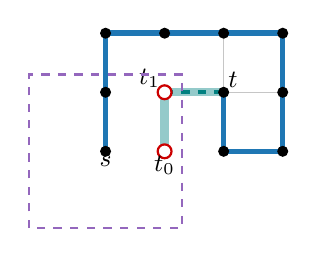
\begin{tikzpicture}[scale=0.75]
\draw[gedge] (0,0) -- (0,1);
\draw[gedge] (0,1) -- (0,2);
\draw[gedge] (0,2) -- (1,2);
\draw[gedge] (1,2) -- (2,2);
\draw[gedge] (2,0) -- (3,0);
\draw[gedge] (2,0) -- (2,1);
\draw[gedge] (2,1) -- (3,1);
\draw[gedge] (2,1) -- (2,2);
\draw[gedge] (2,2) -- (3,2);
\draw[gedge] (3,0) -- (3,1);
\draw[gedge] (3,1) -- (3,2);
\draw[pc1] (0,0) -- (0,1);
\draw[pc1] (0,1) -- (0,2);
\draw[pc1] (0,2) -- (1,2);
\draw[pc1] (1,2) -- (2,2);
\draw[pc1] (2,2) -- (3,2);
\draw[pc1] (3,1) -- (3,2);
\draw[pc1] (3,0) -- (3,1);
\draw[pc1] (2,0) -- (3,0);
\draw[pc1] (2,0) -- (2,1);
\draw[delpath] (1,1) -- (2,1);
\draw[delpath] (1,0) -- (1,1);
\draw[ph] (1,1) -- (2,1);
\node[pt] at (0,0) {};
\node[pt] at (0,1) {};
\node[pt] at (0,2) {};
\node[pt] at (1,2) {};
\node[pt] at (2,0) {};
\node[pt] at (2,1) {};
\node[pt] at (2,2) {};
\node[pt] at (3,0) {};
\node[pt] at (3,1) {};
\node[pt] at (3,2) {};
\node[miss] at (1,0) {};
\node[miss] at (1,1) {};
\node[lab,below] at (0,0) {$s$};
\node[lab,below] at (1,0) {$t_0$};
\node[lab,above left] at (1,1) {$t_1$};
\node[lab,above right] at (2,1) {$t$};
\draw[king] (-1.3,-1.3) rectangle (1.3,1.3);
\end{tikzpicture}\qquad\qquad
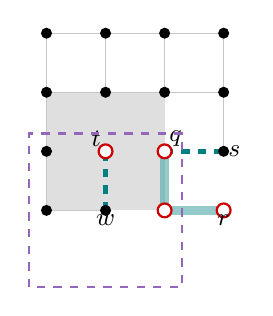
\begin{tikzpicture}[scale=0.75]
\fill[holecell] (0,0) rectangle (1,1);
\fill[holecell] (1,0) rectangle (2,1);
\fill[holecell] (0,1) rectangle (1,2);
\fill[holecell] (1,1) rectangle (2,2);
\draw[gedge] (0,0) -- (1,0);
\draw[gedge] (0,0) -- (0,1);
\draw[gedge] (0,1) -- (0,2);
\draw[gedge] (0,2) -- (1,2);
\draw[gedge] (0,2) -- (0,3);
\draw[gedge] (0,3) -- (1,3);
\draw[gedge] (1,2) -- (2,2);
\draw[gedge] (1,2) -- (1,3);
\draw[gedge] (1,3) -- (2,3);
\draw[gedge] (2,2) -- (3,2);
\draw[gedge] (2,2) -- (2,3);
\draw[gedge] (2,3) -- (3,3);
\draw[gedge] (3,1) -- (3,2);
\draw[gedge] (3,2) -- (3,3);
\draw[delpath] (2,0) -- (3,0);
\draw[delpath] (2,0) -- (2,1);
\draw[ph] (1,0) -- (1,1);
\draw[ph] (2,1) -- (3,1);
\node[pt] at (0,0) {};
\node[pt] at (0,1) {};
\node[pt] at (0,2) {};
\node[pt] at (0,3) {};
\node[pt] at (1,0) {};
\node[pt] at (1,2) {};
\node[pt] at (1,3) {};
\node[pt] at (2,2) {};
\node[pt] at (2,3) {};
\node[pt] at (3,1) {};
\node[pt] at (3,2) {};
\node[pt] at (3,3) {};
\node[miss] at (1,1) {};
\node[miss] at (3,0) {};
\node[miss] at (2,0) {};
\node[miss] at (2,1) {};
\node[lab,above left] at (1,1) {$t$};
\node[lab,below] at (1,0) {$w$};
\node[lab,below] at (3,0) {$r$};
\node[lab,below] at (2,0) {};
\node[lab,above right] at (2,1) {$q$};
\node[lab,right] at (3,1) {$s$};
\draw[king] (-0.3,-1.3) rectangle (2.3,1.3);
\end{tikzpicture}

\caption{Left: the deletion walk with two boundary endpoints.
The Hamiltonian path from $s$ to $t_0$ ends with $t,t_1,t_0$, and its deleted part is teal.
The walk deletes $t_0$ and then $t_1$, because each lies inside the purple box (king distance at
most $1$ from $s$).
The endpoint $t$ is outside the box, so $s,t$ are Far.
The deleted $t_1$ is a usable phantom of $t$.
Right: the $s$-side walk in the $4\times4$ instance of \cref{sec:inside} (\cref{sec:one}).
The inner endpoint $t$ has been deleted (grey hole cells) and $w$ is its neighbour on the path.
The deleted path $P$ (teal) runs from $r$ (the original $s$) to the phantom $q$.
The current endpoint $s$ is joined to $q$ by a phantom edge (dashed).
The purple box holds the points within king distance $1$ of $w$.}
\label{fig:walk}
\end{figure}

% =====================================================================
\section{Inner endpoints: holes, vortices and slit heights}
\label{sec:vortex}

An inner endpoint has no missing king neighbour, so no phantom is available.
The algorithm deletes it anyway.

\begin{definition}[hole]
Let $t$ be inner in the solid set $V$, and let $w$ be the neighbour of $t$ on a Hamiltonian path.
Put $V'=V\setminus\{t\}$.
The point $t$ is a \emph{hole} of $V'$, because all eight of its king neighbours lie in $V'$.
The four squares with corner $t$ are the \emph{hole cells}.
They are cells of $V$ but not of $V'$, so they are never flipped.
The point $t$ is the phantom of $w$.
\end{definition}

Two facts that solidity gave now fail.
There is no height (this section), and factors need not be connected by flips (\cref{sec:classes}).

\begin{definition}[vortex]
A \emph{vortex} of $H$ is a point of degree $1$ that is inner in the original solid set.
\end{definition}

At a vortex the four arcs do not balance.
Going once around it, they add up to $\pm2$ (\lean{wS\_defect1}).
So no height exists on the cells of $V$.
In a phantom factor for the inner endpoint, $t$ has degree $1$ (its only edge is $w$--$t$), so $t$
is a vortex.

\begin{definition}[slit]
The \emph{slit} of a vortex $(a,b)$ is the set of horizontal edges on row $b$ strictly left of $a$
(Lean \lean{SlitE}).
\end{definition}

\begin{theorem}[slit height, \lean{slit\_height}, \lean{SlitHeight.lean}]
\label{thm:slit}
Let $V$ be solid, let $(a,b)$ be inner with $\deg_H(a,b)=1$, and let every other inner point have
degree $2$.
Then there are $\tau\colon\Z^2\to\Z$ and $\delta\in\{2,-2\}$ such that for every side $e$ between two
cells of $V$
\[
  \tau(c^+)-\tau(c^-)
  = \varepsilon(e)+\begin{cases}\delta & \text{if $e$ is in the slit,}\\ 0&\text{otherwise.}\end{cases}
\]
Here $c^-$ is the lower or left square of $e$, $c^+$ the upper or right one, and $\varepsilon(e)$ is
$+1$ if the arc of $H$ across $e$ points from $c^-$ to $c^+$ and $-1$ otherwise.
\end{theorem}

The proof routes the imbalance $\delta$ as a unit flow from the vortex straight left past all of
$V$, and subtracts it (\cref{app:slit}).
\Cref{fig:twistrun} in \cref{app:runs} shows slit heights during a run.

\begin{definition}[quadrant label]
For a vortex $(a,b)$ and a square $c=(x,y)$, $\lab(c)$ is $0$ if $y<b$ and $x<a$, $1$ if $y<b$ and
$x\ge a$, $2$ if $y\ge b$ and $x\ge a$, and $3$ if $y\ge b$ and $x<a$ (Lean \lean{lab}).
\end{definition}

The four squares around the vortex have labels $0,1,2,3$ counterclockwise from the lower left.
Across the vertical line through the vortex and across the ray right of it, the label changes by
$\pm1$.
Across the slit it changes by $\pm3$ (\lean{lab\_step}, \cref{fig:vortex}).

\begin{figure}[t]
\centering
% SPDX-License-Identifier: CC0-1.0
% Generated by gen.py; do not edit by hand.
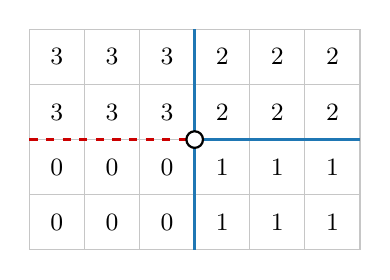
\begin{tikzpicture}[scale=0.7]
\node[clab] at (0+0.5,0+0.5) {0};
\node[clab] at (0+0.5,1+0.5) {0};
\node[clab] at (0+0.5,2+0.5) {3};
\node[clab] at (0+0.5,3+0.5) {3};
\node[clab] at (1+0.5,0+0.5) {0};
\node[clab] at (1+0.5,1+0.5) {0};
\node[clab] at (1+0.5,2+0.5) {3};
\node[clab] at (1+0.5,3+0.5) {3};
\node[clab] at (2+0.5,0+0.5) {0};
\node[clab] at (2+0.5,1+0.5) {0};
\node[clab] at (2+0.5,2+0.5) {3};
\node[clab] at (2+0.5,3+0.5) {3};
\node[clab] at (3+0.5,0+0.5) {1};
\node[clab] at (3+0.5,1+0.5) {1};
\node[clab] at (3+0.5,2+0.5) {2};
\node[clab] at (3+0.5,3+0.5) {2};
\node[clab] at (4+0.5,0+0.5) {1};
\node[clab] at (4+0.5,1+0.5) {1};
\node[clab] at (4+0.5,2+0.5) {2};
\node[clab] at (4+0.5,3+0.5) {2};
\node[clab] at (5+0.5,0+0.5) {1};
\node[clab] at (5+0.5,1+0.5) {1};
\node[clab] at (5+0.5,2+0.5) {2};
\node[clab] at (5+0.5,3+0.5) {2};
\draw[gedge] (0,0) grid (6,4);
\draw[bnd] (3,0) -- (3,4);
\draw[bnd] (3,2) -- (6,2);
\draw[slit] (0,2) -- (3,2);
\node[vort] at (3,2) {};
\end{tikzpicture}\qquad
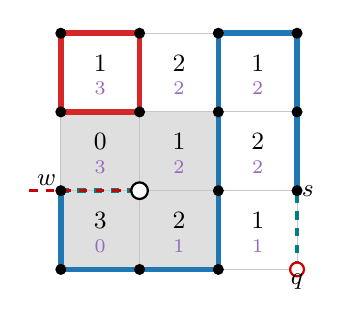
\begin{tikzpicture}[scale=1.0]
\fill[holecell] (0,0) rectangle (1,1);
\fill[holecell] (1,0) rectangle (2,1);
\fill[holecell] (0,1) rectangle (1,2);
\fill[holecell] (1,1) rectangle (2,2);
\draw[gedge] (0,0) -- (1,0);
\draw[gedge] (0,0) -- (0,1);
\draw[gedge] (0,1) -- (1,1);
\draw[gedge] (0,1) -- (0,2);
\draw[gedge] (0,2) -- (1,2);
\draw[gedge] (0,2) -- (0,3);
\draw[gedge] (0,3) -- (1,3);
\draw[gedge] (1,0) -- (2,0);
\draw[gedge] (1,0) -- (1,1);
\draw[gedge] (1,1) -- (2,1);
\draw[gedge] (1,1) -- (1,2);
\draw[gedge] (1,2) -- (2,2);
\draw[gedge] (1,2) -- (1,3);
\draw[gedge] (1,3) -- (2,3);
\draw[gedge] (2,0) -- (3,0);
\draw[gedge] (2,0) -- (2,1);
\draw[gedge] (2,1) -- (3,1);
\draw[gedge] (2,1) -- (2,2);
\draw[gedge] (2,2) -- (3,2);
\draw[gedge] (2,2) -- (2,3);
\draw[gedge] (2,3) -- (3,3);
\draw[gedge] (3,0) -- (3,1);
\draw[gedge] (3,1) -- (3,2);
\draw[gedge] (3,2) -- (3,3);
\draw[pc1] (0,0) -- (0,1);
\draw[pc1] (0,0) -- (1,0);
\draw[pc1] (1,0) -- (2,0);
\draw[pc1] (2,0) -- (2,1);
\draw[pc1] (2,1) -- (2,2);
\draw[pc1] (2,2) -- (2,3);
\draw[pc1] (2,3) -- (3,3);
\draw[pc1] (3,2) -- (3,3);
\draw[pc1] (3,1) -- (3,2);
\draw[pc2] (0,2) -- (1,2);
\draw[pc2] (1,2) -- (1,3);
\draw[pc2] (0,3) -- (1,3);
\draw[pc2] (0,2) -- (0,3);
\draw[ph] (0,1) -- (1,1);
\draw[ph] (3,0) -- (3,1);
\draw[slit] (-0.4,1) -- (1,1);
\node[taulab] at (0+0.5,0+0.62) {$3$};
\node[qlab] at (0+0.5,0+0.3) {0};
\node[taulab] at (1+0.5,0+0.62) {$2$};
\node[qlab] at (1+0.5,0+0.3) {1};
\node[taulab] at (2+0.5,0+0.62) {$1$};
\node[qlab] at (2+0.5,0+0.3) {1};
\node[taulab] at (0+0.5,1+0.62) {$0$};
\node[qlab] at (0+0.5,1+0.3) {3};
\node[taulab] at (1+0.5,1+0.62) {$1$};
\node[qlab] at (1+0.5,1+0.3) {2};
\node[taulab] at (2+0.5,1+0.62) {$2$};
\node[qlab] at (2+0.5,1+0.3) {2};
\node[taulab] at (0+0.5,2+0.62) {$1$};
\node[qlab] at (0+0.5,2+0.3) {3};
\node[taulab] at (1+0.5,2+0.62) {$2$};
\node[qlab] at (1+0.5,2+0.3) {2};
\node[taulab] at (2+0.5,2+0.62) {$1$};
\node[qlab] at (2+0.5,2+0.3) {2};
\node[pt] at (0,0) {};
\node[pt] at (0,1) {};
\node[pt] at (0,2) {};
\node[pt] at (0,3) {};
\node[pt] at (1,0) {};
\node[pt] at (1,2) {};
\node[pt] at (1,3) {};
\node[pt] at (2,0) {};
\node[pt] at (2,1) {};
\node[pt] at (2,2) {};
\node[pt] at (2,3) {};
\node[pt] at (3,1) {};
\node[pt] at (3,2) {};
\node[pt] at (3,3) {};
\node[vort] at (1,1) {};
\node[miss] at (3,0) {};
\node[lab,above left] at (0,1) {$w$};
\node[lab,right] at (3,1) {$s$};
\node[lab,below] at (3,0) {$q$};
\end{tikzpicture}

\caption{Left: the quadrant label around a vortex (open circle).
It changes by $\pm1$ across the blue lines and by $\pm3$ across the slit (red dashed).
Right: the factor $G_0$ of the $4\times4$ instance of \cref{sec:inside}.
The open circle is the deleted inner endpoint $t$, a vortex of the factor.
Each cell shows its slit height $\tau$ (bold, shifted so the least value is $0$) and its quadrant
label (small, purple).
The slit is the single side left of $t$ on its row.
Here $\delta=-2$, and the function $2\tau+\lab$ rises along every arc (\cref{sec:inside}).}
\label{fig:vortex}
\end{figure}

\begin{theorem}[no closed climb around a vortex, \lean{arc\_vortex}]
\label{thm:vortex}
Under the hypotheses of \cref{thm:slit}, $H$ has no closed walk of arc steps between cells of $V$
in a fixed direction.
In particular \lean{ClimbAcyc}~$V\ H$ holds (\lean{acyc\_vortex}).
\end{theorem}

\begin{proof}
Fix the direction $o$ and put $g=1$ for $o=\lean{true}$ and $g=-1$ otherwise.
Take $\tau,\delta$ from \cref{thm:slit}.
Put $\nu=-1$ if $g\delta=2$ and $\nu=1$ if $g\delta=-2$, and
\[\Phi(c)=2g\,\tau(c)+\nu\,\lab(c).\]
Consider a step from $c$ to $c'$ whose arc points in direction $o$.
For a function $f$ on squares write $\Delta f=f(c')-f(c)$ for the change of $f$ along this step.
By \cref{thm:slit}, $g(\tau(c')-\tau(c))=1+g\kappa$ where $\kappa$ is $\delta$ for an upward
crossing of the slit, $-\delta$ for a downward crossing, and $0$ otherwise.
\begin{itemize}
\item Away from the slit, $2g\Delta\tau=2$ and $|\Delta\lab|\le1$, so $\Delta\Phi\ge1$.
\item Upward across the slit, $\Delta\lab=+3$ and $2g\Delta\tau=2+2g\delta$.
  If $g\delta=2$ then $\nu=-1$ and $\Delta\Phi=6-3=3$.
  If $g\delta=-2$ then $\nu=1$ and $\Delta\Phi=-2+3=1$.
\item Downward across the slit, $\Delta\lab=-3$ and $2g\Delta\tau=2-2g\delta$.
  If $g\delta=2$ then $\Delta\Phi=-2+3=1$.
  If $g\delta=-2$ then $\Delta\Phi=6-3=3$.
\end{itemize}
So $\Phi$ rises strictly along every step, and a closed walk would return $\Phi$ to its start value.
\end{proof}

The proof uses only the local inequality $\Delta\Phi\ge1$ across each arc.
It does not argue about which cells a closed walk encloses, so no planar topology (such as the
Jordan curve theorem) is needed, which keeps the Lean proof elementary.
\lean{arcAcyc\_transfer} passes the conclusion to a subset of the cells and to any factor whose arcs
agree on the sides between those cells.

% =====================================================================
\section{Classes and the class search}
\label{sec:classes}

With a hole, two factors with the same degrees need not be connected by cell flips.
Sheffield's Theorem~8~\cite[\S4.1]{sheffield2000} indexes the flip components of $2$-factors on a
grid graph with holes by the relative height on the holes.
The classes below follow this idea.
They are taken relative to phantom and deleted endpoints, and the degree-one defect is handled by
\cref{sec:vortex}.
Throughout this section $U$ is the current set of a leaf, the original $V$ without the deleted
points (\cref{sec:one,sec:two}), and in the simplest case $U=V'=V\setminus\{t\}$.
A factor of the leaf lives on $W=U\cup\{t,q\}$, with phantom edges $w$--$t$ and from the current
endpoint to its phantom $q$.

\paragraph{An informal picture.}
Fix a path factor $F$.
Every other path factor $G$ can be described by a height map $\varphi$ on the cells, defined
precisely below.
$\varphi$ is $0$ outside the bounding box.
Contiguous cells of equal height form regions, and the boundary between two regions is a
\emph{fence}.
Walking along a fence, its edges alternately lie in $F$ and not in $F$.
$G$ is $F\oplus X$, where $X$ is the set of edges of all the fences of $\varphi$.
$\varphi$ changes by exactly $\pm1$ when crossing a fence.
The sign is set by the arcs of $F$ across the fence, which all point the same way, and $\varphi$
rises by $1$ when crossing in the direction of these arcs.

The height of $\varphi$ at the hole is called the \emph{class} of $G$.
It can be interpreted as the number of fences that enclose, or loop around, the hole.
Each such fence counts $+1$ if the arcs of $F$ across it point toward the hole and $-1$ if they
point away from it.
Other fences, or loops, can be present, but since they do not encircle the hole they do not change
the class.
If there is no room to fit the class number of fences around the hole, the class is \emph{empty}
and can be rejected from consideration for a Hamiltonian path.
Finding $\varphi$ for a given class starts by assigning the class to the hole cell $t$.
The other cells then follow by a Bellman--Ford relaxation of the constraints \emph{step $0$ or $+1$
in the direction of the arc of $F$}, which raises every cell to the least value the constraints allow
(\cref{fig:classsearch}).

Put together, the algorithm runs Sheffield's loop once for every possible number $h$ of fences
around the hole, with $h$ counted with its sign.
Since $|h|\le|U|$ (\cref{thm:classsearch}), at most $2|U|+1$ values need to be tried, and $(2|U|+1)^2$ pairs with two holes.
For each value the relaxation either finds a factor of that class, which is then the starting factor
of the loop for that class, or shows that the class is empty.
If any factor of the class exists, the relaxation finds one, so no class that could hold a
Hamiltonian path is skipped.

\begin{definition}[reference factor, class]
Fix a factor $F$ of the leaf (the \emph{reference factor}).
For a factor $G$ that agrees with $F$ off the edges of $U$, the \emph{class} of $G$ is
$h(G)=D(F,G)(t)/2\in\Z$, read at the hole cell $t$ (Lean \lean{classSearchOne}, \lean{class\_mem\_hRange}).
With two holes $t$ and $r$ the class is the pair $(D(F,G)(t)/2,\,D(F,G)(r)/2)$.
\end{definition}

All four hole cells carry the same value of $D(F,G)$, since no edge at $t$ lies in $F\oplus G$.
Since $F\oplus G$ is a union of alternating cycles and $D(F,G)$ changes by $\pm2$ exactly across
its edges, $h(G)$ is the signed number of these cycles that go around the hole.

\paragraph{Classes in an example.}
\Cref{fig:classes} shows a leaf of the $4\times5$ block with $s=(1,0)$ and inner $t=(2,2)$.
In this leaf the neighbour of $t$ on the path is $w=(3,2)$ and the successor of $s$ is $x=(0,0)$
(\cref{sec:one}).
Its factors fall into exactly two classes, $h=0$ and $h=1$.
The least factors $G_0$ and $G_1$ of the two classes differ by a single alternating $12$-cycle, which
goes around the hole (\cref{fig:classes}c).
Inside this cycle $D(G_0,G_1)/2=1$, and in particular it is $1$ on the four hole cells.
No sequence of flips turns $G_0$ into $G_1$, because a flip changes $D$ only on the flipped cell and
the hole cells are never flipped.
The final test treats the two classes separately.
It runs \lean{classSearchOne} for $h=-18,\dots,18$, which returns nothing except for $h=0$ and $h=1$.
For $h=0$ the loop starts from $G_0$ with $2$ pieces, flips one merging cell, and reaches one piece,
so this leaf has a Hamiltonian path.
Had $h=0$ failed, the test would go on to $h=1$.
There the first phase from $G_1$ is stuck with $2$ pieces, and the certificate shows that no factor
of class $1$ has one piece.

\begin{figure}[t]
\centering
% SPDX-License-Identifier: CC0-1.0
% Generated by gen.py; do not edit by hand.
\begin{tabular}{c@{\qquad}c@{\qquad}c}
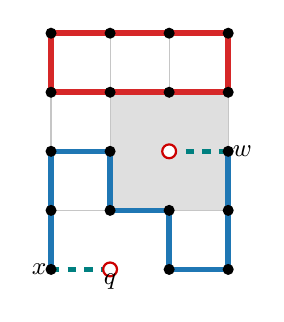
\begin{tikzpicture}[scale=0.75]
\fill[holecell] (1,1) rectangle (2,2);
\fill[holecell] (2,1) rectangle (3,2);
\fill[holecell] (1,2) rectangle (2,3);
\fill[holecell] (2,2) rectangle (3,3);
\draw[gedge] (0,0) -- (0,1);
\draw[gedge] (0,1) -- (1,1);
\draw[gedge] (0,1) -- (0,2);
\draw[gedge] (0,2) -- (1,2);
\draw[gedge] (0,2) -- (0,3);
\draw[gedge] (0,3) -- (1,3);
\draw[gedge] (0,3) -- (0,4);
\draw[gedge] (0,4) -- (1,4);
\draw[gedge] (1,1) -- (2,1);
\draw[gedge] (1,1) -- (1,2);
\draw[gedge] (1,2) -- (1,3);
\draw[gedge] (1,3) -- (2,3);
\draw[gedge] (1,3) -- (1,4);
\draw[gedge] (1,4) -- (2,4);
\draw[gedge] (2,0) -- (3,0);
\draw[gedge] (2,0) -- (2,1);
\draw[gedge] (2,1) -- (3,1);
\draw[gedge] (2,3) -- (3,3);
\draw[gedge] (2,3) -- (2,4);
\draw[gedge] (2,4) -- (3,4);
\draw[gedge] (3,0) -- (3,1);
\draw[gedge] (3,1) -- (3,2);
\draw[gedge] (3,2) -- (3,3);
\draw[gedge] (3,3) -- (3,4);
\draw[pc1] (0,2) -- (1,2);
\draw[pc1] (1,1) -- (2,1);
\draw[pc1] (2,0) -- (3,0);
\draw[pc1] (0,0) -- (0,1);
\draw[pc1] (0,1) -- (0,2);
\draw[pc1] (1,1) -- (1,2);
\draw[pc1] (2,0) -- (2,1);
\draw[pc1] (3,0) -- (3,1);
\draw[pc1] (3,1) -- (3,2);
\draw[pc2] (0,3) -- (1,3);
\draw[pc2] (0,4) -- (1,4);
\draw[pc2] (1,3) -- (2,3);
\draw[pc2] (1,4) -- (2,4);
\draw[pc2] (2,3) -- (3,3);
\draw[pc2] (2,4) -- (3,4);
\draw[pc2] (0,3) -- (0,4);
\draw[pc2] (3,3) -- (3,4);
\draw[ph] (2,2) -- (3,2);
\draw[ph] (0,0) -- (1,0);
\node[pt] at (0,0) {};
\node[pt] at (0,1) {};
\node[pt] at (0,2) {};
\node[pt] at (0,3) {};
\node[pt] at (0,4) {};
\node[pt] at (1,1) {};
\node[pt] at (1,2) {};
\node[pt] at (1,3) {};
\node[pt] at (1,4) {};
\node[pt] at (2,0) {};
\node[pt] at (2,1) {};
\node[pt] at (2,3) {};
\node[pt] at (2,4) {};
\node[pt] at (3,0) {};
\node[pt] at (3,1) {};
\node[pt] at (3,2) {};
\node[pt] at (3,3) {};
\node[pt] at (3,4) {};
\node[miss] at (1,0) {};
\node[miss] at (2,2) {};
\node[lab,right] at (3,2) {$w$};
\node[lab,left] at (0,0) {$x$};
\node[lab,below] at (1,0) {$q$};
\end{tikzpicture} & 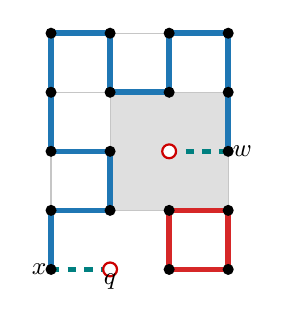
\begin{tikzpicture}[scale=0.75]
\fill[holecell] (1,1) rectangle (2,2);
\fill[holecell] (2,1) rectangle (3,2);
\fill[holecell] (1,2) rectangle (2,3);
\fill[holecell] (2,2) rectangle (3,3);
\draw[gedge] (0,0) -- (0,1);
\draw[gedge] (0,1) -- (1,1);
\draw[gedge] (0,1) -- (0,2);
\draw[gedge] (0,2) -- (1,2);
\draw[gedge] (0,2) -- (0,3);
\draw[gedge] (0,3) -- (1,3);
\draw[gedge] (0,3) -- (0,4);
\draw[gedge] (0,4) -- (1,4);
\draw[gedge] (1,1) -- (2,1);
\draw[gedge] (1,1) -- (1,2);
\draw[gedge] (1,2) -- (1,3);
\draw[gedge] (1,3) -- (2,3);
\draw[gedge] (1,3) -- (1,4);
\draw[gedge] (1,4) -- (2,4);
\draw[gedge] (2,0) -- (3,0);
\draw[gedge] (2,0) -- (2,1);
\draw[gedge] (2,1) -- (3,1);
\draw[gedge] (2,3) -- (3,3);
\draw[gedge] (2,3) -- (2,4);
\draw[gedge] (2,4) -- (3,4);
\draw[gedge] (3,0) -- (3,1);
\draw[gedge] (3,1) -- (3,2);
\draw[gedge] (3,2) -- (3,3);
\draw[gedge] (3,3) -- (3,4);
\draw[pc1] (0,1) -- (1,1);
\draw[pc1] (0,2) -- (1,2);
\draw[pc1] (0,4) -- (1,4);
\draw[pc1] (1,3) -- (2,3);
\draw[pc1] (2,4) -- (3,4);
\draw[pc1] (0,0) -- (0,1);
\draw[pc1] (0,2) -- (0,3);
\draw[pc1] (0,3) -- (0,4);
\draw[pc1] (1,1) -- (1,2);
\draw[pc1] (1,3) -- (1,4);
\draw[pc1] (2,3) -- (2,4);
\draw[pc1] (3,2) -- (3,3);
\draw[pc1] (3,3) -- (3,4);
\draw[pc2] (2,0) -- (3,0);
\draw[pc2] (2,1) -- (3,1);
\draw[pc2] (2,0) -- (2,1);
\draw[pc2] (3,0) -- (3,1);
\draw[ph] (2,2) -- (3,2);
\draw[ph] (0,0) -- (1,0);
\node[pt] at (0,0) {};
\node[pt] at (0,1) {};
\node[pt] at (0,2) {};
\node[pt] at (0,3) {};
\node[pt] at (0,4) {};
\node[pt] at (1,1) {};
\node[pt] at (1,2) {};
\node[pt] at (1,3) {};
\node[pt] at (1,4) {};
\node[pt] at (2,0) {};
\node[pt] at (2,1) {};
\node[pt] at (2,3) {};
\node[pt] at (2,4) {};
\node[pt] at (3,0) {};
\node[pt] at (3,1) {};
\node[pt] at (3,2) {};
\node[pt] at (3,3) {};
\node[pt] at (3,4) {};
\node[miss] at (1,0) {};
\node[miss] at (2,2) {};
\node[lab,right] at (3,2) {$w$};
\node[lab,left] at (0,0) {$x$};
\node[lab,below] at (1,0) {$q$};
\end{tikzpicture} & 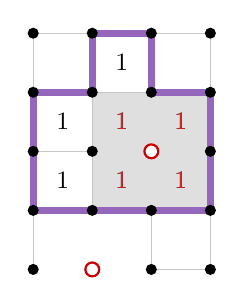
\begin{tikzpicture}[scale=0.75]
\fill[holecell] (1,1) rectangle (2,2);
\fill[holecell] (2,1) rectangle (3,2);
\fill[holecell] (1,2) rectangle (2,3);
\fill[holecell] (2,2) rectangle (3,3);
\draw[gedge] (0,0) -- (0,1);
\draw[gedge] (0,1) -- (1,1);
\draw[gedge] (0,1) -- (0,2);
\draw[gedge] (0,2) -- (1,2);
\draw[gedge] (0,2) -- (0,3);
\draw[gedge] (0,3) -- (1,3);
\draw[gedge] (0,3) -- (0,4);
\draw[gedge] (0,4) -- (1,4);
\draw[gedge] (1,1) -- (2,1);
\draw[gedge] (1,1) -- (1,2);
\draw[gedge] (1,2) -- (1,3);
\draw[gedge] (1,3) -- (2,3);
\draw[gedge] (1,3) -- (1,4);
\draw[gedge] (1,4) -- (2,4);
\draw[gedge] (2,0) -- (3,0);
\draw[gedge] (2,0) -- (2,1);
\draw[gedge] (2,1) -- (3,1);
\draw[gedge] (2,3) -- (3,3);
\draw[gedge] (2,3) -- (2,4);
\draw[gedge] (2,4) -- (3,4);
\draw[gedge] (3,0) -- (3,1);
\draw[gedge] (3,1) -- (3,2);
\draw[gedge] (3,2) -- (3,3);
\draw[gedge] (3,3) -- (3,4);
\draw[xedge] (0,1) -- (1,1);
\draw[xedge] (0,3) -- (1,3);
\draw[xedge] (1,1) -- (2,1);
\draw[xedge] (1,4) -- (2,4);
\draw[xedge] (2,1) -- (3,1);
\draw[xedge] (2,3) -- (3,3);
\draw[xedge] (0,1) -- (0,2);
\draw[xedge] (0,2) -- (0,3);
\draw[xedge] (1,3) -- (1,4);
\draw[xedge] (2,3) -- (2,4);
\draw[xedge] (3,1) -- (3,2);
\draw[xedge] (3,2) -- (3,3);
\node[pt] at (0,0) {};
\node[pt] at (0,1) {};
\node[pt] at (0,2) {};
\node[pt] at (0,3) {};
\node[pt] at (0,4) {};
\node[pt] at (1,1) {};
\node[pt] at (1,2) {};
\node[pt] at (1,3) {};
\node[pt] at (1,4) {};
\node[pt] at (2,0) {};
\node[pt] at (2,1) {};
\node[pt] at (2,3) {};
\node[pt] at (2,4) {};
\node[pt] at (3,0) {};
\node[pt] at (3,1) {};
\node[pt] at (3,2) {};
\node[pt] at (3,3) {};
\node[pt] at (3,4) {};
\node[miss] at (1,0) {};
\node[miss] at (2,2) {};
\node[taulab] at (0+0.5,1+0.5) {$1$};
\node[taulab] at (0+0.5,2+0.5) {$1$};
\node[taulab] at (1+0.5,1+0.5) {$1$};
\node[taulab] at (1+0.5,2+0.5) {$1$};
\node[taulab] at (1+0.5,3+0.5) {$1$};
\node[taulab] at (2+0.5,1+0.5) {$1$};
\node[taulab] at (2+0.5,2+0.5) {$1$};
\node[taulab,pcB] at (1+0.5,1+0.5) {$1$};
\node[taulab,pcB] at (2+0.5,1+0.5) {$1$};
\node[taulab,pcB] at (1+0.5,2+0.5) {$1$};
\node[taulab,pcB] at (2+0.5,2+0.5) {$1$};
\end{tikzpicture} \\
\small (a) class $h=0$ & \small (b) class $h=1$ & \small (c) $G_0\oplus G_1$, $D/2$
\end{tabular}

\caption{Two classes at one leaf.
$V$ is the $4\times5$ block, $s=(1,0)$ (deleted, the phantom $q$) and the inner endpoint $t=(2,2)$
(deleted, grey hole cells).
(a) The least factor $G_0$ of class $h=0$, with $2$ pieces.
(b) The least factor $G_1$ of class $h=1$, with $2$ pieces.
(c) $G_0\oplus G_1$ (purple) is one alternating cycle around the hole.
Each cell inside it shows $D(G_0,G_1)/2=1$, and the hole cells show $1$ in red.
The loop succeeds in class $0$ and is stuck in class $1$.}
\label{fig:classes}
\end{figure}

\begin{lemma}[class implies \lean{SolidFor}, \lean{solidFor\_of\_holes}]
\label{lem:classsolid}
Let every missing point of $U$ be joined by king moves through missing points to a hole or to a
point left of $U$, as the walk invariant \lean{WS} of \cref{sec:one} provides.
If two factors $G$ and $G'$ of the leaf have the same class, then $D(G,G')(c)=0$ for every square
$c$ that is not a cell of
$U$.
\end{lemma}

The proof is in \cref{app:class}.
\Cref{lem:classsolid} supplies exactly the hypothesis \lean{SolidFor} of \cref{thm:cert}.

\begin{lemma}[the run keeps its class, \lean{sf\_flip}, \lean{sf\_flipCol}, \lean{sf\_reduceOutC2}, \lean{HoleRun.lean}, \lean{HoleTwo.lean}]
\label{lem:runclass}
A flip of an alternating cell keeps $D(\cdot,X)$ off the flipped cell, for every $X$ with the same
degrees.
Every flip made by the loop is of an alternating cell.
So every state of a run has the class of its start.
\end{lemma}

\begin{proof}
Let $G'$ be $G$ with an alternating cell $c$ flipped, so $G$, $G'$ and $X$ have the same degrees.
The proof of \cref{lem:D} shows that $D(A,B)$ jumps across each side by
$\varepsilon_A-\varepsilon_B$.
So $D(G',X)-D(G,X)$ and $D(G',G)$ have the same jumps and are both $0$ far left, hence equal.
The vertical edges of $G\oplus G'$ are the left and right sides of $c$.
They have the same membership, so by \cref{def:arc} their arcs both point into $c$ or both point out
of $c$, that is, in opposite horizontal directions, and their weights cancel.
By \cref{def:D}, $D(G',G)$ is therefore $0$ on every square except $c$.
Every flip of the loop is of an alternating cell.
A merging cell is alternating by definition.
A bridge end $E$ has dark laterals and light back and front when it is flipped, and dark back and
front and light laterals when it is flipped back, so it is alternating both times.
Lowering a row flips its cells from the last down to the first, and each is alternating when it is
flipped (\lean{sf\_flipCol}).
The hole cells are not cells of $U$ and are never flipped, so $D(F,\cdot)=-D(\cdot,F)$ keeps its
value at the hole cells, and the class does not change.
\end{proof}

The class is kept flip by flip.
Toggling an alternating cycle around the hole, which is not a sequence of cell flips, changes it.

\paragraph{The class search.}
Factors $G$ that agree with $F$ off the edges of $U$ correspond one to one to \emph{admissible
potentials} (Lean \lean{Adm}, \lean{HoleAdm.lean}).
An admissible potential is an integer function $\varphi$ on squares, zero outside the bounding box,
whose jump across every side is $0$, except that across an edge $e$ of $U$ it may equal the sign of
the arc of $F$ across $e$.
The factor is $G=F\oplus X_\varphi$ where $X_\varphi$ is the set of edges of $U$ across which
$\varphi$ jumps, and $D(F,G)=2\varphi$.
Prescribing $\varphi(t)=h$ adds one more difference constraint.
\lean{classSearch} relaxes from below to the least admissible potential with the prescribed values, checks
it, and returns $F\oplus X_\varphi$ (\lean{Algorithm.lean}).
\lean{classSearchOne}~$U\ F\ t\ h$ is \lean{classSearch} with one prescribed value.

\paragraph{How the relaxation runs.}
The unknowns are the values $\varphi(c)$ on the squares $c$ of the bounding box (\lean{boxSquares}).
Squares outside the box keep the value $0$.
For a side $e$ between a lower or left square $c^-$ and an upper or right square $c^+$, the rule
\emph{jump $0$ or the sign $\sigma(e)$ of the arc of $F$} becomes the two inequalities
\[\min(0,\sigma(e))\le\varphi(c^+)-\varphi(c^-)\le\max(0,\sigma(e)),\]
and a side that is not an edge of $U$ gets $0\le\varphi(c^+)-\varphi(c^-)\le0$.
The prescribed hole cell starts at $h$ and every other square at $-\omega$, where $\omega$ is the width of the
box (\lean{kInitA}).
No admissible potential is lower than $-\omega$, because it is $0$ outside the box and changes by at most
$1$ from one square to the next.
A round raises every square, all at once, to the largest value that its four sides force from the
current values of its neighbours, or keeps it when that is lower (\lean{lowerBound},
\lean{roundA}).
Values only rise, and the hole cell can rise above $h$ as well.
The rounds stop when nothing changes, at the latest after $|S|+1$ rounds (\lean{relax\_bf}, below).
If some admissible potential $\psi$ with value $h$ at the hole exists, every round stays at or below
$\psi$, so the fixed point satisfies every inequality and still has the value $h$ at the hole.
\lean{isAdmissible} checks exactly these two facts (\lean{relax\_fix}, \lean{check\_iff}).
When the check fails the class is empty.

\Cref{fig:classsearch} runs the search on a leaf of the $7\times5$ block.
The factors of this leaf fall into three classes, $h=-1,0,1$.
In each the least potential is a plateau of height $h$ around the hole, and the boundary of the
plateau is an alternating cycle of $F\oplus G$ around the hole.
Other contours, such as the $-1$ cells of class $0$, do not go around the hole and leave the class
unchanged.
For $h=2$ the values forced around the hole reach the boundary of the box, where the step rule fails
on nine sides, so the class is empty.
In this leaf the loop reaches one piece in every nonempty class.
In the leaf of \cref{fig:classes} the loop succeeds in class $0$ and is stuck in class $1$.

\begin{figure}[p]
\centering
% SPDX-License-Identifier: CC0-1.0
% Generated by gen.py; do not edit by hand.
\begin{tabular}{c@{\quad}c@{\quad}c}
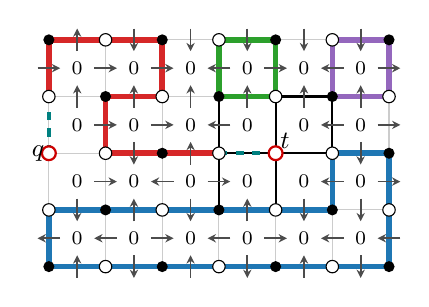
\begin{tikzpicture}[scale=0.72]
\draw[gray!40] (0,0) grid (6,4);
\draw[black,thick] (3,1) rectangle (4,2);
\draw[black,thick] (4,1) rectangle (5,2);
\draw[black,thick] (3,2) rectangle (4,3);
\draw[black,thick] (4,2) rectangle (5,3);
\draw[pc1] (0,0) -- (1,0);
\draw[pc1] (0,1) -- (1,1);
\draw[pc1] (1,0) -- (2,0);
\draw[pc1] (1,1) -- (2,1);
\draw[pc1] (2,0) -- (3,0);
\draw[pc1] (2,1) -- (3,1);
\draw[pc1] (3,0) -- (4,0);
\draw[pc1] (3,1) -- (4,1);
\draw[pc1] (4,0) -- (5,0);
\draw[pc1] (4,1) -- (5,1);
\draw[pc1] (5,0) -- (6,0);
\draw[pc1] (5,2) -- (6,2);
\draw[pc1] (0,0) -- (0,1);
\draw[pc1] (5,1) -- (5,2);
\draw[pc1] (6,0) -- (6,1);
\draw[pc1] (6,1) -- (6,2);
\draw[pc2] (0,4) -- (1,4);
\draw[pc2] (1,2) -- (2,2);
\draw[pc2] (1,3) -- (2,3);
\draw[pc2] (1,4) -- (2,4);
\draw[pc2] (2,2) -- (3,2);
\draw[pc2] (0,3) -- (0,4);
\draw[pc2] (1,2) -- (1,3);
\draw[pc2] (2,3) -- (2,4);
\draw[pc3] (3,3) -- (4,3);
\draw[pc3] (3,4) -- (4,4);
\draw[pc3] (3,3) -- (3,4);
\draw[pc3] (4,3) -- (4,4);
\draw[pc4] (5,3) -- (6,3);
\draw[pc4] (5,4) -- (6,4);
\draw[pc4] (5,3) -- (5,4);
\draw[pc4] (6,3) -- (6,4);
\draw[ph] (3,2) -- (4,2);
\draw[ph] (0,2) -- (0,3);
\draw[arcarrowsm] (0.20,0.50) -- (-0.20,0.50);
\draw[arcarrowsm] (-0.20,3.50) -- (0.20,3.50);
\draw[arcarrowsm] (0.50,-0.20) -- (0.50,0.20);
\draw[arcarrowsm] (0.50,1.20) -- (0.50,0.80);
\draw[arcarrowsm] (1.20,0.50) -- (0.80,0.50);
\draw[arcarrowsm] (0.80,1.50) -- (1.20,1.50);
\draw[arcarrowsm] (0.50,2.80) -- (0.50,3.20);
\draw[arcarrowsm] (0.80,2.50) -- (1.20,2.50);
\draw[arcarrowsm] (0.50,3.80) -- (0.50,4.20);
\draw[arcarrowsm] (0.80,3.50) -- (1.20,3.50);
\draw[arcarrowsm] (1.50,0.20) -- (1.50,-0.20);
\draw[arcarrowsm] (1.50,0.80) -- (1.50,1.20);
\draw[arcarrowsm] (1.80,0.50) -- (2.20,0.50);
\draw[arcarrowsm] (1.50,2.20) -- (1.50,1.80);
\draw[arcarrowsm] (2.20,1.50) -- (1.80,1.50);
\draw[arcarrowsm] (1.50,2.80) -- (1.50,3.20);
\draw[arcarrowsm] (1.80,2.50) -- (2.20,2.50);
\draw[arcarrowsm] (1.50,4.20) -- (1.50,3.80);
\draw[arcarrowsm] (1.80,3.50) -- (2.20,3.50);
\draw[arcarrowsm] (2.50,-0.20) -- (2.50,0.20);
\draw[arcarrowsm] (2.50,1.20) -- (2.50,0.80);
\draw[arcarrowsm] (3.20,0.50) -- (2.80,0.50);
\draw[arcarrowsm] (2.50,1.80) -- (2.50,2.20);
\draw[arcarrowsm] (2.80,1.50) -- (3.20,1.50);
\draw[arcarrowsm] (2.50,2.80) -- (2.50,3.20);
\draw[arcarrowsm] (3.20,2.50) -- (2.80,2.50);
\draw[arcarrowsm] (2.50,4.20) -- (2.50,3.80);
\draw[arcarrowsm] (3.20,3.50) -- (2.80,3.50);
\draw[arcarrowsm] (3.50,0.20) -- (3.50,-0.20);
\draw[arcarrowsm] (3.50,0.80) -- (3.50,1.20);
\draw[arcarrowsm] (3.80,0.50) -- (4.20,0.50);
\draw[arcarrowsm] (3.50,2.80) -- (3.50,3.20);
\draw[arcarrowsm] (3.50,4.20) -- (3.50,3.80);
\draw[arcarrowsm] (3.80,3.50) -- (4.20,3.50);
\draw[arcarrowsm] (4.50,-0.20) -- (4.50,0.20);
\draw[arcarrowsm] (4.50,1.20) -- (4.50,0.80);
\draw[arcarrowsm] (5.20,0.50) -- (4.80,0.50);
\draw[arcarrowsm] (5.20,1.50) -- (4.80,1.50);
\draw[arcarrowsm] (4.50,2.80) -- (4.50,3.20);
\draw[arcarrowsm] (5.20,2.50) -- (4.80,2.50);
\draw[arcarrowsm] (4.50,4.20) -- (4.50,3.80);
\draw[arcarrowsm] (5.20,3.50) -- (4.80,3.50);
\draw[arcarrowsm] (5.50,0.20) -- (5.50,-0.20);
\draw[arcarrowsm] (5.50,1.20) -- (5.50,0.80);
\draw[arcarrowsm] (6.20,0.50) -- (5.80,0.50);
\draw[arcarrowsm] (5.50,2.20) -- (5.50,1.80);
\draw[arcarrowsm] (5.80,1.50) -- (6.20,1.50);
\draw[arcarrowsm] (5.50,2.80) -- (5.50,3.20);
\draw[arcarrowsm] (5.80,2.50) -- (6.20,2.50);
\draw[arcarrowsm] (5.50,4.20) -- (5.50,3.80);
\draw[arcarrowsm] (5.80,3.50) -- (6.20,3.50);
\node[font=\scriptsize,fill=white,fill opacity=0.6,text opacity=1,inner sep=0.5pt] at (0+0.5,0+0.5) {$0$};
\node[font=\scriptsize,fill=white,fill opacity=0.6,text opacity=1,inner sep=0.5pt] at (0+0.5,1+0.5) {$0$};
\node[font=\scriptsize,fill=white,fill opacity=0.6,text opacity=1,inner sep=0.5pt] at (0+0.5,2+0.5) {$0$};
\node[font=\scriptsize,fill=white,fill opacity=0.6,text opacity=1,inner sep=0.5pt] at (0+0.5,3+0.5) {$0$};
\node[font=\scriptsize,fill=white,fill opacity=0.6,text opacity=1,inner sep=0.5pt] at (1+0.5,0+0.5) {$0$};
\node[font=\scriptsize,fill=white,fill opacity=0.6,text opacity=1,inner sep=0.5pt] at (1+0.5,1+0.5) {$0$};
\node[font=\scriptsize,fill=white,fill opacity=0.6,text opacity=1,inner sep=0.5pt] at (1+0.5,2+0.5) {$0$};
\node[font=\scriptsize,fill=white,fill opacity=0.6,text opacity=1,inner sep=0.5pt] at (1+0.5,3+0.5) {$0$};
\node[font=\scriptsize,fill=white,fill opacity=0.6,text opacity=1,inner sep=0.5pt] at (2+0.5,0+0.5) {$0$};
\node[font=\scriptsize,fill=white,fill opacity=0.6,text opacity=1,inner sep=0.5pt] at (2+0.5,1+0.5) {$0$};
\node[font=\scriptsize,fill=white,fill opacity=0.6,text opacity=1,inner sep=0.5pt] at (2+0.5,2+0.5) {$0$};
\node[font=\scriptsize,fill=white,fill opacity=0.6,text opacity=1,inner sep=0.5pt] at (2+0.5,3+0.5) {$0$};
\node[font=\scriptsize,fill=white,fill opacity=0.6,text opacity=1,inner sep=0.5pt] at (3+0.5,0+0.5) {$0$};
\node[font=\scriptsize,fill=white,fill opacity=0.6,text opacity=1,inner sep=0.5pt] at (3+0.5,1+0.5) {$0$};
\node[font=\scriptsize,fill=white,fill opacity=0.6,text opacity=1,inner sep=0.5pt] at (3+0.5,2+0.5) {$0$};
\node[font=\scriptsize,fill=white,fill opacity=0.6,text opacity=1,inner sep=0.5pt] at (3+0.5,3+0.5) {$0$};
\node[font=\scriptsize,fill=white,fill opacity=0.6,text opacity=1,inner sep=0.5pt] at (4+0.5,0+0.5) {$0$};
\node[font=\scriptsize,fill=white,fill opacity=0.6,text opacity=1,inner sep=0.5pt] at (4+0.5,1+0.5) {$0$};
\node[font=\scriptsize,fill=white,fill opacity=0.6,text opacity=1,inner sep=0.5pt] at (4+0.5,2+0.5) {$0$};
\node[font=\scriptsize,fill=white,fill opacity=0.6,text opacity=1,inner sep=0.5pt] at (4+0.5,3+0.5) {$0$};
\node[font=\scriptsize,fill=white,fill opacity=0.6,text opacity=1,inner sep=0.5pt] at (5+0.5,0+0.5) {$0$};
\node[font=\scriptsize,fill=white,fill opacity=0.6,text opacity=1,inner sep=0.5pt] at (5+0.5,1+0.5) {$0$};
\node[font=\scriptsize,fill=white,fill opacity=0.6,text opacity=1,inner sep=0.5pt] at (5+0.5,2+0.5) {$0$};
\node[font=\scriptsize,fill=white,fill opacity=0.6,text opacity=1,inner sep=0.5pt] at (5+0.5,3+0.5) {$0$};
\node[pt] at (0,0) {};
\node[wpt] at (0,1) {};
\node[wpt] at (0,3) {};
\node[pt] at (0,4) {};
\node[wpt] at (1,0) {};
\node[pt] at (1,1) {};
\node[wpt] at (1,2) {};
\node[pt] at (1,3) {};
\node[wpt] at (1,4) {};
\node[pt] at (2,0) {};
\node[wpt] at (2,1) {};
\node[pt] at (2,2) {};
\node[wpt] at (2,3) {};
\node[pt] at (2,4) {};
\node[wpt] at (3,0) {};
\node[pt] at (3,1) {};
\node[wpt] at (3,2) {};
\node[pt] at (3,3) {};
\node[wpt] at (3,4) {};
\node[pt] at (4,0) {};
\node[wpt] at (4,1) {};
\node[wpt] at (4,3) {};
\node[pt] at (4,4) {};
\node[wpt] at (5,0) {};
\node[pt] at (5,1) {};
\node[wpt] at (5,2) {};
\node[pt] at (5,3) {};
\node[wpt] at (5,4) {};
\node[pt] at (6,0) {};
\node[wpt] at (6,1) {};
\node[pt] at (6,2) {};
\node[wpt] at (6,3) {};
\node[pt] at (6,4) {};
\node[miss] at (0,2) {};
\node[miss] at (4,2) {};
\node[lab,above right] at (4,2) {$t$};
\node[lab,left] at (0,2) {$q$};
\end{tikzpicture} & 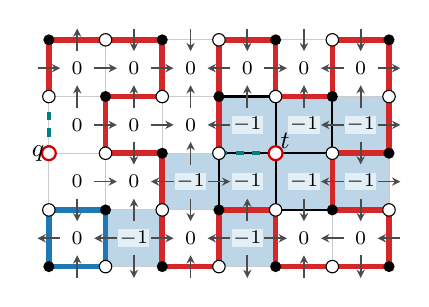
\begin{tikzpicture}[scale=0.72]
\fill[pcA!30] (1,0) rectangle (2,1);
\fill[pcA!30] (2,1) rectangle (3,2);
\fill[pcA!30] (3,0) rectangle (4,1);
\fill[pcA!30] (3,1) rectangle (4,2);
\fill[pcA!30] (3,2) rectangle (4,3);
\fill[pcA!30] (4,1) rectangle (5,2);
\fill[pcA!30] (4,2) rectangle (5,3);
\fill[pcA!30] (5,1) rectangle (6,2);
\fill[pcA!30] (5,2) rectangle (6,3);
\draw[gray!40] (0,0) grid (6,4);
\draw[black,thick] (3,1) rectangle (4,2);
\draw[black,thick] (4,1) rectangle (5,2);
\draw[black,thick] (3,2) rectangle (4,3);
\draw[black,thick] (4,2) rectangle (5,3);
\draw[pc1] (0,0) -- (1,0);
\draw[pc1] (0,1) -- (1,1);
\draw[pc1] (0,0) -- (0,1);
\draw[pc1] (1,0) -- (1,1);
\draw[pc2] (0,4) -- (1,4);
\draw[pc2] (1,2) -- (2,2);
\draw[pc2] (1,3) -- (2,3);
\draw[pc2] (1,4) -- (2,4);
\draw[pc2] (2,0) -- (3,0);
\draw[pc2] (3,1) -- (4,1);
\draw[pc2] (3,4) -- (4,4);
\draw[pc2] (4,0) -- (5,0);
\draw[pc2] (4,3) -- (5,3);
\draw[pc2] (5,0) -- (6,0);
\draw[pc2] (5,1) -- (6,1);
\draw[pc2] (5,2) -- (6,2);
\draw[pc2] (5,4) -- (6,4);
\draw[pc2] (0,3) -- (0,4);
\draw[pc2] (1,2) -- (1,3);
\draw[pc2] (2,0) -- (2,1);
\draw[pc2] (2,1) -- (2,2);
\draw[pc2] (2,3) -- (2,4);
\draw[pc2] (3,0) -- (3,1);
\draw[pc2] (3,2) -- (3,3);
\draw[pc2] (3,3) -- (3,4);
\draw[pc2] (4,0) -- (4,1);
\draw[pc2] (4,3) -- (4,4);
\draw[pc2] (5,1) -- (5,2);
\draw[pc2] (5,3) -- (5,4);
\draw[pc2] (6,0) -- (6,1);
\draw[pc2] (6,2) -- (6,3);
\draw[pc2] (6,3) -- (6,4);
\draw[ph] (3,2) -- (4,2);
\draw[ph] (0,2) -- (0,3);
\draw[arcarrowsm] (0.20,0.50) -- (-0.20,0.50);
\draw[arcarrowsm] (-0.20,3.50) -- (0.20,3.50);
\draw[arcarrowsm] (0.50,-0.20) -- (0.50,0.20);
\draw[arcarrowsm] (0.50,1.20) -- (0.50,0.80);
\draw[arcarrowsm] (1.20,0.50) -- (0.80,0.50);
\draw[arcarrowsm] (0.80,1.50) -- (1.20,1.50);
\draw[arcarrowsm] (0.50,2.80) -- (0.50,3.20);
\draw[arcarrowsm] (0.80,2.50) -- (1.20,2.50);
\draw[arcarrowsm] (0.50,3.80) -- (0.50,4.20);
\draw[arcarrowsm] (0.80,3.50) -- (1.20,3.50);
\draw[arcarrowsm] (1.50,0.20) -- (1.50,-0.20);
\draw[arcarrowsm] (1.50,0.80) -- (1.50,1.20);
\draw[arcarrowsm] (1.80,0.50) -- (2.20,0.50);
\draw[arcarrowsm] (1.50,2.20) -- (1.50,1.80);
\draw[arcarrowsm] (2.20,1.50) -- (1.80,1.50);
\draw[arcarrowsm] (1.50,2.80) -- (1.50,3.20);
\draw[arcarrowsm] (1.80,2.50) -- (2.20,2.50);
\draw[arcarrowsm] (1.50,4.20) -- (1.50,3.80);
\draw[arcarrowsm] (1.80,3.50) -- (2.20,3.50);
\draw[arcarrowsm] (2.50,-0.20) -- (2.50,0.20);
\draw[arcarrowsm] (2.50,1.20) -- (2.50,0.80);
\draw[arcarrowsm] (3.20,0.50) -- (2.80,0.50);
\draw[arcarrowsm] (2.50,1.80) -- (2.50,2.20);
\draw[arcarrowsm] (2.80,1.50) -- (3.20,1.50);
\draw[arcarrowsm] (2.50,2.80) -- (2.50,3.20);
\draw[arcarrowsm] (3.20,2.50) -- (2.80,2.50);
\draw[arcarrowsm] (2.50,4.20) -- (2.50,3.80);
\draw[arcarrowsm] (3.20,3.50) -- (2.80,3.50);
\draw[arcarrowsm] (3.50,0.20) -- (3.50,-0.20);
\draw[arcarrowsm] (3.50,0.80) -- (3.50,1.20);
\draw[arcarrowsm] (3.80,0.50) -- (4.20,0.50);
\draw[arcarrowsm] (3.50,2.80) -- (3.50,3.20);
\draw[arcarrowsm] (3.50,4.20) -- (3.50,3.80);
\draw[arcarrowsm] (3.80,3.50) -- (4.20,3.50);
\draw[arcarrowsm] (4.50,-0.20) -- (4.50,0.20);
\draw[arcarrowsm] (4.50,1.20) -- (4.50,0.80);
\draw[arcarrowsm] (5.20,0.50) -- (4.80,0.50);
\draw[arcarrowsm] (5.20,1.50) -- (4.80,1.50);
\draw[arcarrowsm] (4.50,2.80) -- (4.50,3.20);
\draw[arcarrowsm] (5.20,2.50) -- (4.80,2.50);
\draw[arcarrowsm] (4.50,4.20) -- (4.50,3.80);
\draw[arcarrowsm] (5.20,3.50) -- (4.80,3.50);
\draw[arcarrowsm] (5.50,0.20) -- (5.50,-0.20);
\draw[arcarrowsm] (5.50,1.20) -- (5.50,0.80);
\draw[arcarrowsm] (6.20,0.50) -- (5.80,0.50);
\draw[arcarrowsm] (5.50,2.20) -- (5.50,1.80);
\draw[arcarrowsm] (5.80,1.50) -- (6.20,1.50);
\draw[arcarrowsm] (5.50,2.80) -- (5.50,3.20);
\draw[arcarrowsm] (5.80,2.50) -- (6.20,2.50);
\draw[arcarrowsm] (5.50,4.20) -- (5.50,3.80);
\draw[arcarrowsm] (5.80,3.50) -- (6.20,3.50);
\node[font=\scriptsize,fill=white,fill opacity=0.6,text opacity=1,inner sep=0.5pt] at (0+0.5,0+0.5) {$0$};
\node[font=\scriptsize,fill=white,fill opacity=0.6,text opacity=1,inner sep=0.5pt] at (0+0.5,1+0.5) {$0$};
\node[font=\scriptsize,fill=white,fill opacity=0.6,text opacity=1,inner sep=0.5pt] at (0+0.5,2+0.5) {$0$};
\node[font=\scriptsize,fill=white,fill opacity=0.6,text opacity=1,inner sep=0.5pt] at (0+0.5,3+0.5) {$0$};
\node[font=\scriptsize,fill=white,fill opacity=0.6,text opacity=1,inner sep=0.5pt] at (1+0.5,0+0.5) {$-1$};
\node[font=\scriptsize,fill=white,fill opacity=0.6,text opacity=1,inner sep=0.5pt] at (1+0.5,1+0.5) {$0$};
\node[font=\scriptsize,fill=white,fill opacity=0.6,text opacity=1,inner sep=0.5pt] at (1+0.5,2+0.5) {$0$};
\node[font=\scriptsize,fill=white,fill opacity=0.6,text opacity=1,inner sep=0.5pt] at (1+0.5,3+0.5) {$0$};
\node[font=\scriptsize,fill=white,fill opacity=0.6,text opacity=1,inner sep=0.5pt] at (2+0.5,0+0.5) {$0$};
\node[font=\scriptsize,fill=white,fill opacity=0.6,text opacity=1,inner sep=0.5pt] at (2+0.5,1+0.5) {$-1$};
\node[font=\scriptsize,fill=white,fill opacity=0.6,text opacity=1,inner sep=0.5pt] at (2+0.5,2+0.5) {$0$};
\node[font=\scriptsize,fill=white,fill opacity=0.6,text opacity=1,inner sep=0.5pt] at (2+0.5,3+0.5) {$0$};
\node[font=\scriptsize,fill=white,fill opacity=0.6,text opacity=1,inner sep=0.5pt] at (3+0.5,0+0.5) {$-1$};
\node[font=\scriptsize,fill=white,fill opacity=0.6,text opacity=1,inner sep=0.5pt] at (3+0.5,1+0.5) {$-1$};
\node[font=\scriptsize,fill=white,fill opacity=0.6,text opacity=1,inner sep=0.5pt] at (3+0.5,2+0.5) {$-1$};
\node[font=\scriptsize,fill=white,fill opacity=0.6,text opacity=1,inner sep=0.5pt] at (3+0.5,3+0.5) {$0$};
\node[font=\scriptsize,fill=white,fill opacity=0.6,text opacity=1,inner sep=0.5pt] at (4+0.5,0+0.5) {$0$};
\node[font=\scriptsize,fill=white,fill opacity=0.6,text opacity=1,inner sep=0.5pt] at (4+0.5,1+0.5) {$-1$};
\node[font=\scriptsize,fill=white,fill opacity=0.6,text opacity=1,inner sep=0.5pt] at (4+0.5,2+0.5) {$-1$};
\node[font=\scriptsize,fill=white,fill opacity=0.6,text opacity=1,inner sep=0.5pt] at (4+0.5,3+0.5) {$0$};
\node[font=\scriptsize,fill=white,fill opacity=0.6,text opacity=1,inner sep=0.5pt] at (5+0.5,0+0.5) {$0$};
\node[font=\scriptsize,fill=white,fill opacity=0.6,text opacity=1,inner sep=0.5pt] at (5+0.5,1+0.5) {$-1$};
\node[font=\scriptsize,fill=white,fill opacity=0.6,text opacity=1,inner sep=0.5pt] at (5+0.5,2+0.5) {$-1$};
\node[font=\scriptsize,fill=white,fill opacity=0.6,text opacity=1,inner sep=0.5pt] at (5+0.5,3+0.5) {$0$};
\node[pt] at (0,0) {};
\node[wpt] at (0,1) {};
\node[wpt] at (0,3) {};
\node[pt] at (0,4) {};
\node[wpt] at (1,0) {};
\node[pt] at (1,1) {};
\node[wpt] at (1,2) {};
\node[pt] at (1,3) {};
\node[wpt] at (1,4) {};
\node[pt] at (2,0) {};
\node[wpt] at (2,1) {};
\node[pt] at (2,2) {};
\node[wpt] at (2,3) {};
\node[pt] at (2,4) {};
\node[wpt] at (3,0) {};
\node[pt] at (3,1) {};
\node[wpt] at (3,2) {};
\node[pt] at (3,3) {};
\node[wpt] at (3,4) {};
\node[pt] at (4,0) {};
\node[wpt] at (4,1) {};
\node[wpt] at (4,3) {};
\node[pt] at (4,4) {};
\node[wpt] at (5,0) {};
\node[pt] at (5,1) {};
\node[wpt] at (5,2) {};
\node[pt] at (5,3) {};
\node[wpt] at (5,4) {};
\node[pt] at (6,0) {};
\node[wpt] at (6,1) {};
\node[pt] at (6,2) {};
\node[wpt] at (6,3) {};
\node[pt] at (6,4) {};
\node[miss] at (0,2) {};
\node[miss] at (4,2) {};
\node[lab,above right] at (4,2) {$t$};
\node[lab,left] at (0,2) {$q$};
\end{tikzpicture} & 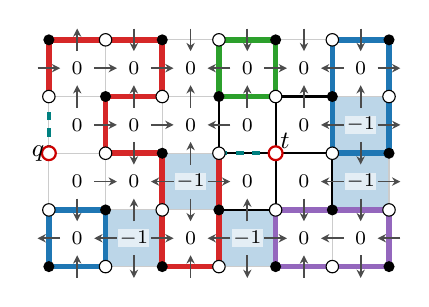
\begin{tikzpicture}[scale=0.72]
\fill[pcA!30] (1,0) rectangle (2,1);
\fill[pcA!30] (2,1) rectangle (3,2);
\fill[pcA!30] (3,0) rectangle (4,1);
\fill[pcA!30] (5,1) rectangle (6,2);
\fill[pcA!30] (5,2) rectangle (6,3);
\draw[gray!40] (0,0) grid (6,4);
\draw[black,thick] (3,1) rectangle (4,2);
\draw[black,thick] (4,1) rectangle (5,2);
\draw[black,thick] (3,2) rectangle (4,3);
\draw[black,thick] (4,2) rectangle (5,3);
\draw[pc1] (0,0) -- (1,0);
\draw[pc1] (0,1) -- (1,1);
\draw[pc1] (0,0) -- (0,1);
\draw[pc1] (1,0) -- (1,1);
\draw[pc2] (0,4) -- (1,4);
\draw[pc2] (1,2) -- (2,2);
\draw[pc2] (1,3) -- (2,3);
\draw[pc2] (1,4) -- (2,4);
\draw[pc2] (2,0) -- (3,0);
\draw[pc2] (0,3) -- (0,4);
\draw[pc2] (1,2) -- (1,3);
\draw[pc2] (2,0) -- (2,1);
\draw[pc2] (2,1) -- (2,2);
\draw[pc2] (2,3) -- (2,4);
\draw[pc2] (3,0) -- (3,1);
\draw[pc2] (3,1) -- (3,2);
\draw[pc3] (3,3) -- (4,3);
\draw[pc3] (3,4) -- (4,4);
\draw[pc3] (3,3) -- (3,4);
\draw[pc3] (4,3) -- (4,4);
\draw[pc4] (4,0) -- (5,0);
\draw[pc4] (4,1) -- (5,1);
\draw[pc4] (5,0) -- (6,0);
\draw[pc4] (5,1) -- (6,1);
\draw[pc4] (4,0) -- (4,1);
\draw[pc4] (6,0) -- (6,1);
\draw[pc1] (5,2) -- (6,2);
\draw[pc1] (5,4) -- (6,4);
\draw[pc1] (5,2) -- (5,3);
\draw[pc1] (5,3) -- (5,4);
\draw[pc1] (6,2) -- (6,3);
\draw[pc1] (6,3) -- (6,4);
\draw[ph] (3,2) -- (4,2);
\draw[ph] (0,2) -- (0,3);
\draw[arcarrowsm] (0.20,0.50) -- (-0.20,0.50);
\draw[arcarrowsm] (-0.20,3.50) -- (0.20,3.50);
\draw[arcarrowsm] (0.50,-0.20) -- (0.50,0.20);
\draw[arcarrowsm] (0.50,1.20) -- (0.50,0.80);
\draw[arcarrowsm] (1.20,0.50) -- (0.80,0.50);
\draw[arcarrowsm] (0.80,1.50) -- (1.20,1.50);
\draw[arcarrowsm] (0.50,2.80) -- (0.50,3.20);
\draw[arcarrowsm] (0.80,2.50) -- (1.20,2.50);
\draw[arcarrowsm] (0.50,3.80) -- (0.50,4.20);
\draw[arcarrowsm] (0.80,3.50) -- (1.20,3.50);
\draw[arcarrowsm] (1.50,0.20) -- (1.50,-0.20);
\draw[arcarrowsm] (1.50,0.80) -- (1.50,1.20);
\draw[arcarrowsm] (1.80,0.50) -- (2.20,0.50);
\draw[arcarrowsm] (1.50,2.20) -- (1.50,1.80);
\draw[arcarrowsm] (2.20,1.50) -- (1.80,1.50);
\draw[arcarrowsm] (1.50,2.80) -- (1.50,3.20);
\draw[arcarrowsm] (1.80,2.50) -- (2.20,2.50);
\draw[arcarrowsm] (1.50,4.20) -- (1.50,3.80);
\draw[arcarrowsm] (1.80,3.50) -- (2.20,3.50);
\draw[arcarrowsm] (2.50,-0.20) -- (2.50,0.20);
\draw[arcarrowsm] (2.50,1.20) -- (2.50,0.80);
\draw[arcarrowsm] (3.20,0.50) -- (2.80,0.50);
\draw[arcarrowsm] (2.50,1.80) -- (2.50,2.20);
\draw[arcarrowsm] (2.80,1.50) -- (3.20,1.50);
\draw[arcarrowsm] (2.50,2.80) -- (2.50,3.20);
\draw[arcarrowsm] (3.20,2.50) -- (2.80,2.50);
\draw[arcarrowsm] (2.50,4.20) -- (2.50,3.80);
\draw[arcarrowsm] (3.20,3.50) -- (2.80,3.50);
\draw[arcarrowsm] (3.50,0.20) -- (3.50,-0.20);
\draw[arcarrowsm] (3.50,0.80) -- (3.50,1.20);
\draw[arcarrowsm] (3.80,0.50) -- (4.20,0.50);
\draw[arcarrowsm] (3.50,2.80) -- (3.50,3.20);
\draw[arcarrowsm] (3.50,4.20) -- (3.50,3.80);
\draw[arcarrowsm] (3.80,3.50) -- (4.20,3.50);
\draw[arcarrowsm] (4.50,-0.20) -- (4.50,0.20);
\draw[arcarrowsm] (4.50,1.20) -- (4.50,0.80);
\draw[arcarrowsm] (5.20,0.50) -- (4.80,0.50);
\draw[arcarrowsm] (5.20,1.50) -- (4.80,1.50);
\draw[arcarrowsm] (4.50,2.80) -- (4.50,3.20);
\draw[arcarrowsm] (5.20,2.50) -- (4.80,2.50);
\draw[arcarrowsm] (4.50,4.20) -- (4.50,3.80);
\draw[arcarrowsm] (5.20,3.50) -- (4.80,3.50);
\draw[arcarrowsm] (5.50,0.20) -- (5.50,-0.20);
\draw[arcarrowsm] (5.50,1.20) -- (5.50,0.80);
\draw[arcarrowsm] (6.20,0.50) -- (5.80,0.50);
\draw[arcarrowsm] (5.50,2.20) -- (5.50,1.80);
\draw[arcarrowsm] (5.80,1.50) -- (6.20,1.50);
\draw[arcarrowsm] (5.50,2.80) -- (5.50,3.20);
\draw[arcarrowsm] (5.80,2.50) -- (6.20,2.50);
\draw[arcarrowsm] (5.50,4.20) -- (5.50,3.80);
\draw[arcarrowsm] (5.80,3.50) -- (6.20,3.50);
\node[font=\scriptsize,fill=white,fill opacity=0.6,text opacity=1,inner sep=0.5pt] at (0+0.5,0+0.5) {$0$};
\node[font=\scriptsize,fill=white,fill opacity=0.6,text opacity=1,inner sep=0.5pt] at (0+0.5,1+0.5) {$0$};
\node[font=\scriptsize,fill=white,fill opacity=0.6,text opacity=1,inner sep=0.5pt] at (0+0.5,2+0.5) {$0$};
\node[font=\scriptsize,fill=white,fill opacity=0.6,text opacity=1,inner sep=0.5pt] at (0+0.5,3+0.5) {$0$};
\node[font=\scriptsize,fill=white,fill opacity=0.6,text opacity=1,inner sep=0.5pt] at (1+0.5,0+0.5) {$-1$};
\node[font=\scriptsize,fill=white,fill opacity=0.6,text opacity=1,inner sep=0.5pt] at (1+0.5,1+0.5) {$0$};
\node[font=\scriptsize,fill=white,fill opacity=0.6,text opacity=1,inner sep=0.5pt] at (1+0.5,2+0.5) {$0$};
\node[font=\scriptsize,fill=white,fill opacity=0.6,text opacity=1,inner sep=0.5pt] at (1+0.5,3+0.5) {$0$};
\node[font=\scriptsize,fill=white,fill opacity=0.6,text opacity=1,inner sep=0.5pt] at (2+0.5,0+0.5) {$0$};
\node[font=\scriptsize,fill=white,fill opacity=0.6,text opacity=1,inner sep=0.5pt] at (2+0.5,1+0.5) {$-1$};
\node[font=\scriptsize,fill=white,fill opacity=0.6,text opacity=1,inner sep=0.5pt] at (2+0.5,2+0.5) {$0$};
\node[font=\scriptsize,fill=white,fill opacity=0.6,text opacity=1,inner sep=0.5pt] at (2+0.5,3+0.5) {$0$};
\node[font=\scriptsize,fill=white,fill opacity=0.6,text opacity=1,inner sep=0.5pt] at (3+0.5,0+0.5) {$-1$};
\node[font=\scriptsize,fill=white,fill opacity=0.6,text opacity=1,inner sep=0.5pt] at (3+0.5,1+0.5) {$0$};
\node[font=\scriptsize,fill=white,fill opacity=0.6,text opacity=1,inner sep=0.5pt] at (3+0.5,2+0.5) {$0$};
\node[font=\scriptsize,fill=white,fill opacity=0.6,text opacity=1,inner sep=0.5pt] at (3+0.5,3+0.5) {$0$};
\node[font=\scriptsize,fill=white,fill opacity=0.6,text opacity=1,inner sep=0.5pt] at (4+0.5,0+0.5) {$0$};
\node[font=\scriptsize,fill=white,fill opacity=0.6,text opacity=1,inner sep=0.5pt] at (4+0.5,1+0.5) {$0$};
\node[font=\scriptsize,fill=white,fill opacity=0.6,text opacity=1,inner sep=0.5pt] at (4+0.5,2+0.5) {$0$};
\node[font=\scriptsize,fill=white,fill opacity=0.6,text opacity=1,inner sep=0.5pt] at (4+0.5,3+0.5) {$0$};
\node[font=\scriptsize,fill=white,fill opacity=0.6,text opacity=1,inner sep=0.5pt] at (5+0.5,0+0.5) {$0$};
\node[font=\scriptsize,fill=white,fill opacity=0.6,text opacity=1,inner sep=0.5pt] at (5+0.5,1+0.5) {$-1$};
\node[font=\scriptsize,fill=white,fill opacity=0.6,text opacity=1,inner sep=0.5pt] at (5+0.5,2+0.5) {$-1$};
\node[font=\scriptsize,fill=white,fill opacity=0.6,text opacity=1,inner sep=0.5pt] at (5+0.5,3+0.5) {$0$};
\node[pt] at (0,0) {};
\node[wpt] at (0,1) {};
\node[wpt] at (0,3) {};
\node[pt] at (0,4) {};
\node[wpt] at (1,0) {};
\node[pt] at (1,1) {};
\node[wpt] at (1,2) {};
\node[pt] at (1,3) {};
\node[wpt] at (1,4) {};
\node[pt] at (2,0) {};
\node[wpt] at (2,1) {};
\node[pt] at (2,2) {};
\node[wpt] at (2,3) {};
\node[pt] at (2,4) {};
\node[wpt] at (3,0) {};
\node[pt] at (3,1) {};
\node[wpt] at (3,2) {};
\node[pt] at (3,3) {};
\node[wpt] at (3,4) {};
\node[pt] at (4,0) {};
\node[wpt] at (4,1) {};
\node[wpt] at (4,3) {};
\node[pt] at (4,4) {};
\node[wpt] at (5,0) {};
\node[pt] at (5,1) {};
\node[wpt] at (5,2) {};
\node[pt] at (5,3) {};
\node[wpt] at (5,4) {};
\node[pt] at (6,0) {};
\node[wpt] at (6,1) {};
\node[pt] at (6,2) {};
\node[wpt] at (6,3) {};
\node[pt] at (6,4) {};
\node[miss] at (0,2) {};
\node[miss] at (4,2) {};
\node[lab,above right] at (4,2) {$t$};
\node[lab,left] at (0,2) {$q$};
\end{tikzpicture} \\
\small (a) reference $F$ & \small (b) $h=-1$, 2 pieces & \small (c) $h=0$, 5 pieces
\end{tabular}\\[6pt]
\begin{tabular}{c@{\quad}c}
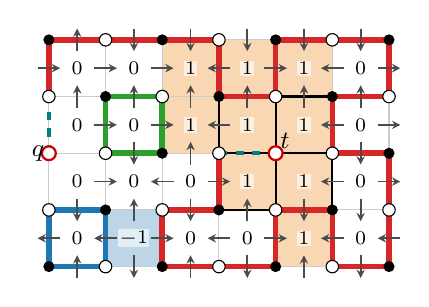
\begin{tikzpicture}[scale=0.72]
\fill[pcA!30] (1,0) rectangle (2,1);
\fill[orng!30] (2,2) rectangle (3,3);
\fill[orng!30] (2,3) rectangle (3,4);
\fill[orng!30] (3,1) rectangle (4,2);
\fill[orng!30] (3,2) rectangle (4,3);
\fill[orng!30] (3,3) rectangle (4,4);
\fill[orng!30] (4,0) rectangle (5,1);
\fill[orng!30] (4,1) rectangle (5,2);
\fill[orng!30] (4,2) rectangle (5,3);
\fill[orng!30] (4,3) rectangle (5,4);
\draw[gray!40] (0,0) grid (6,4);
\draw[black,thick] (3,1) rectangle (4,2);
\draw[black,thick] (4,1) rectangle (5,2);
\draw[black,thick] (3,2) rectangle (4,3);
\draw[black,thick] (4,2) rectangle (5,3);
\draw[pc1] (0,0) -- (1,0);
\draw[pc1] (0,1) -- (1,1);
\draw[pc1] (0,0) -- (0,1);
\draw[pc1] (1,0) -- (1,1);
\draw[pc2] (0,4) -- (1,4);
\draw[pc2] (1,4) -- (2,4);
\draw[pc2] (2,0) -- (3,0);
\draw[pc2] (2,1) -- (3,1);
\draw[pc2] (2,4) -- (3,4);
\draw[pc2] (3,0) -- (4,0);
\draw[pc2] (3,3) -- (4,3);
\draw[pc2] (4,1) -- (5,1);
\draw[pc2] (4,4) -- (5,4);
\draw[pc2] (5,0) -- (6,0);
\draw[pc2] (5,2) -- (6,2);
\draw[pc2] (5,3) -- (6,3);
\draw[pc2] (5,4) -- (6,4);
\draw[pc2] (0,3) -- (0,4);
\draw[pc2] (2,0) -- (2,1);
\draw[pc2] (3,1) -- (3,2);
\draw[pc2] (3,3) -- (3,4);
\draw[pc2] (4,0) -- (4,1);
\draw[pc2] (4,3) -- (4,4);
\draw[pc2] (5,0) -- (5,1);
\draw[pc2] (5,2) -- (5,3);
\draw[pc2] (6,0) -- (6,1);
\draw[pc2] (6,1) -- (6,2);
\draw[pc2] (6,3) -- (6,4);
\draw[pc3] (1,2) -- (2,2);
\draw[pc3] (1,3) -- (2,3);
\draw[pc3] (1,2) -- (1,3);
\draw[pc3] (2,2) -- (2,3);
\draw[ph] (3,2) -- (4,2);
\draw[ph] (0,2) -- (0,3);
\draw[arcarrowsm] (0.20,0.50) -- (-0.20,0.50);
\draw[arcarrowsm] (-0.20,3.50) -- (0.20,3.50);
\draw[arcarrowsm] (0.50,-0.20) -- (0.50,0.20);
\draw[arcarrowsm] (0.50,1.20) -- (0.50,0.80);
\draw[arcarrowsm] (1.20,0.50) -- (0.80,0.50);
\draw[arcarrowsm] (0.80,1.50) -- (1.20,1.50);
\draw[arcarrowsm] (0.50,2.80) -- (0.50,3.20);
\draw[arcarrowsm] (0.80,2.50) -- (1.20,2.50);
\draw[arcarrowsm] (0.50,3.80) -- (0.50,4.20);
\draw[arcarrowsm] (0.80,3.50) -- (1.20,3.50);
\draw[arcarrowsm] (1.50,0.20) -- (1.50,-0.20);
\draw[arcarrowsm] (1.50,0.80) -- (1.50,1.20);
\draw[arcarrowsm] (1.80,0.50) -- (2.20,0.50);
\draw[arcarrowsm] (1.50,2.20) -- (1.50,1.80);
\draw[arcarrowsm] (2.20,1.50) -- (1.80,1.50);
\draw[arcarrowsm] (1.50,2.80) -- (1.50,3.20);
\draw[arcarrowsm] (1.80,2.50) -- (2.20,2.50);
\draw[arcarrowsm] (1.50,4.20) -- (1.50,3.80);
\draw[arcarrowsm] (1.80,3.50) -- (2.20,3.50);
\draw[arcarrowsm] (2.50,-0.20) -- (2.50,0.20);
\draw[arcarrowsm] (2.50,1.20) -- (2.50,0.80);
\draw[arcarrowsm] (3.20,0.50) -- (2.80,0.50);
\draw[arcarrowsm] (2.50,1.80) -- (2.50,2.20);
\draw[arcarrowsm] (2.80,1.50) -- (3.20,1.50);
\draw[arcarrowsm] (2.50,2.80) -- (2.50,3.20);
\draw[arcarrowsm] (3.20,2.50) -- (2.80,2.50);
\draw[arcarrowsm] (2.50,4.20) -- (2.50,3.80);
\draw[arcarrowsm] (3.20,3.50) -- (2.80,3.50);
\draw[arcarrowsm] (3.50,0.20) -- (3.50,-0.20);
\draw[arcarrowsm] (3.50,0.80) -- (3.50,1.20);
\draw[arcarrowsm] (3.80,0.50) -- (4.20,0.50);
\draw[arcarrowsm] (3.50,2.80) -- (3.50,3.20);
\draw[arcarrowsm] (3.50,4.20) -- (3.50,3.80);
\draw[arcarrowsm] (3.80,3.50) -- (4.20,3.50);
\draw[arcarrowsm] (4.50,-0.20) -- (4.50,0.20);
\draw[arcarrowsm] (4.50,1.20) -- (4.50,0.80);
\draw[arcarrowsm] (5.20,0.50) -- (4.80,0.50);
\draw[arcarrowsm] (5.20,1.50) -- (4.80,1.50);
\draw[arcarrowsm] (4.50,2.80) -- (4.50,3.20);
\draw[arcarrowsm] (5.20,2.50) -- (4.80,2.50);
\draw[arcarrowsm] (4.50,4.20) -- (4.50,3.80);
\draw[arcarrowsm] (5.20,3.50) -- (4.80,3.50);
\draw[arcarrowsm] (5.50,0.20) -- (5.50,-0.20);
\draw[arcarrowsm] (5.50,1.20) -- (5.50,0.80);
\draw[arcarrowsm] (6.20,0.50) -- (5.80,0.50);
\draw[arcarrowsm] (5.50,2.20) -- (5.50,1.80);
\draw[arcarrowsm] (5.80,1.50) -- (6.20,1.50);
\draw[arcarrowsm] (5.50,2.80) -- (5.50,3.20);
\draw[arcarrowsm] (5.80,2.50) -- (6.20,2.50);
\draw[arcarrowsm] (5.50,4.20) -- (5.50,3.80);
\draw[arcarrowsm] (5.80,3.50) -- (6.20,3.50);
\node[font=\scriptsize,fill=white,fill opacity=0.6,text opacity=1,inner sep=0.5pt] at (0+0.5,0+0.5) {$0$};
\node[font=\scriptsize,fill=white,fill opacity=0.6,text opacity=1,inner sep=0.5pt] at (0+0.5,1+0.5) {$0$};
\node[font=\scriptsize,fill=white,fill opacity=0.6,text opacity=1,inner sep=0.5pt] at (0+0.5,2+0.5) {$0$};
\node[font=\scriptsize,fill=white,fill opacity=0.6,text opacity=1,inner sep=0.5pt] at (0+0.5,3+0.5) {$0$};
\node[font=\scriptsize,fill=white,fill opacity=0.6,text opacity=1,inner sep=0.5pt] at (1+0.5,0+0.5) {$-1$};
\node[font=\scriptsize,fill=white,fill opacity=0.6,text opacity=1,inner sep=0.5pt] at (1+0.5,1+0.5) {$0$};
\node[font=\scriptsize,fill=white,fill opacity=0.6,text opacity=1,inner sep=0.5pt] at (1+0.5,2+0.5) {$0$};
\node[font=\scriptsize,fill=white,fill opacity=0.6,text opacity=1,inner sep=0.5pt] at (1+0.5,3+0.5) {$0$};
\node[font=\scriptsize,fill=white,fill opacity=0.6,text opacity=1,inner sep=0.5pt] at (2+0.5,0+0.5) {$0$};
\node[font=\scriptsize,fill=white,fill opacity=0.6,text opacity=1,inner sep=0.5pt] at (2+0.5,1+0.5) {$0$};
\node[font=\scriptsize,fill=white,fill opacity=0.6,text opacity=1,inner sep=0.5pt] at (2+0.5,2+0.5) {$1$};
\node[font=\scriptsize,fill=white,fill opacity=0.6,text opacity=1,inner sep=0.5pt] at (2+0.5,3+0.5) {$1$};
\node[font=\scriptsize,fill=white,fill opacity=0.6,text opacity=1,inner sep=0.5pt] at (3+0.5,0+0.5) {$0$};
\node[font=\scriptsize,fill=white,fill opacity=0.6,text opacity=1,inner sep=0.5pt] at (3+0.5,1+0.5) {$1$};
\node[font=\scriptsize,fill=white,fill opacity=0.6,text opacity=1,inner sep=0.5pt] at (3+0.5,2+0.5) {$1$};
\node[font=\scriptsize,fill=white,fill opacity=0.6,text opacity=1,inner sep=0.5pt] at (3+0.5,3+0.5) {$1$};
\node[font=\scriptsize,fill=white,fill opacity=0.6,text opacity=1,inner sep=0.5pt] at (4+0.5,0+0.5) {$1$};
\node[font=\scriptsize,fill=white,fill opacity=0.6,text opacity=1,inner sep=0.5pt] at (4+0.5,1+0.5) {$1$};
\node[font=\scriptsize,fill=white,fill opacity=0.6,text opacity=1,inner sep=0.5pt] at (4+0.5,2+0.5) {$1$};
\node[font=\scriptsize,fill=white,fill opacity=0.6,text opacity=1,inner sep=0.5pt] at (4+0.5,3+0.5) {$1$};
\node[font=\scriptsize,fill=white,fill opacity=0.6,text opacity=1,inner sep=0.5pt] at (5+0.5,0+0.5) {$0$};
\node[font=\scriptsize,fill=white,fill opacity=0.6,text opacity=1,inner sep=0.5pt] at (5+0.5,1+0.5) {$0$};
\node[font=\scriptsize,fill=white,fill opacity=0.6,text opacity=1,inner sep=0.5pt] at (5+0.5,2+0.5) {$0$};
\node[font=\scriptsize,fill=white,fill opacity=0.6,text opacity=1,inner sep=0.5pt] at (5+0.5,3+0.5) {$0$};
\node[pt] at (0,0) {};
\node[wpt] at (0,1) {};
\node[wpt] at (0,3) {};
\node[pt] at (0,4) {};
\node[wpt] at (1,0) {};
\node[pt] at (1,1) {};
\node[wpt] at (1,2) {};
\node[pt] at (1,3) {};
\node[wpt] at (1,4) {};
\node[pt] at (2,0) {};
\node[wpt] at (2,1) {};
\node[pt] at (2,2) {};
\node[wpt] at (2,3) {};
\node[pt] at (2,4) {};
\node[wpt] at (3,0) {};
\node[pt] at (3,1) {};
\node[wpt] at (3,2) {};
\node[pt] at (3,3) {};
\node[wpt] at (3,4) {};
\node[pt] at (4,0) {};
\node[wpt] at (4,1) {};
\node[wpt] at (4,3) {};
\node[pt] at (4,4) {};
\node[wpt] at (5,0) {};
\node[pt] at (5,1) {};
\node[wpt] at (5,2) {};
\node[pt] at (5,3) {};
\node[wpt] at (5,4) {};
\node[pt] at (6,0) {};
\node[wpt] at (6,1) {};
\node[pt] at (6,2) {};
\node[wpt] at (6,3) {};
\node[pt] at (6,4) {};
\node[miss] at (0,2) {};
\node[miss] at (4,2) {};
\node[lab,above right] at (4,2) {$t$};
\node[lab,left] at (0,2) {$q$};
\end{tikzpicture} & 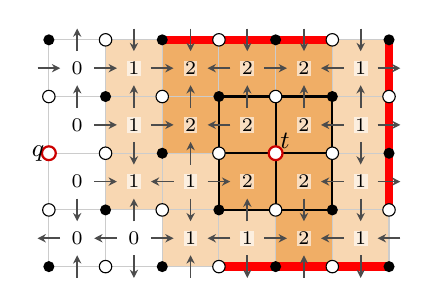
\begin{tikzpicture}[scale=0.72]
\fill[orng!30] (1,1) rectangle (2,2);
\fill[orng!30] (1,2) rectangle (2,3);
\fill[orng!30] (1,3) rectangle (2,4);
\fill[orng!30] (2,0) rectangle (3,1);
\fill[orng!30] (2,1) rectangle (3,2);
\fill[orng!60] (2,2) rectangle (3,3);
\fill[orng!60] (2,3) rectangle (3,4);
\fill[orng!30] (3,0) rectangle (4,1);
\fill[orng!60] (3,1) rectangle (4,2);
\fill[orng!60] (3,2) rectangle (4,3);
\fill[orng!60] (3,3) rectangle (4,4);
\fill[orng!60] (4,0) rectangle (5,1);
\fill[orng!60] (4,1) rectangle (5,2);
\fill[orng!60] (4,2) rectangle (5,3);
\fill[orng!60] (4,3) rectangle (5,4);
\fill[orng!30] (5,0) rectangle (6,1);
\fill[orng!30] (5,1) rectangle (6,2);
\fill[orng!30] (5,2) rectangle (6,3);
\fill[orng!30] (5,3) rectangle (6,4);
\draw[gray!40] (0,0) grid (6,4);
\draw[black,thick] (3,1) rectangle (4,2);
\draw[black,thick] (4,1) rectangle (5,2);
\draw[black,thick] (3,2) rectangle (4,3);
\draw[black,thick] (4,2) rectangle (5,3);
\draw[red,line width=3pt] (2,4) -- (3,4);
\draw[red,line width=3pt] (3,0) -- (4,0);
\draw[red,line width=3pt] (3,4) -- (4,4);
\draw[red,line width=3pt] (4,0) -- (5,0);
\draw[red,line width=3pt] (4,4) -- (5,4);
\draw[red,line width=3pt] (5,0) -- (6,0);
\draw[red,line width=3pt] (6,1) -- (6,2);
\draw[red,line width=3pt] (6,2) -- (6,3);
\draw[red,line width=3pt] (6,3) -- (6,4);
\draw[arcarrowsm] (0.20,0.50) -- (-0.20,0.50);
\draw[arcarrowsm] (-0.20,3.50) -- (0.20,3.50);
\draw[arcarrowsm] (0.50,-0.20) -- (0.50,0.20);
\draw[arcarrowsm] (0.50,1.20) -- (0.50,0.80);
\draw[arcarrowsm] (1.20,0.50) -- (0.80,0.50);
\draw[arcarrowsm] (0.80,1.50) -- (1.20,1.50);
\draw[arcarrowsm] (0.50,2.80) -- (0.50,3.20);
\draw[arcarrowsm] (0.80,2.50) -- (1.20,2.50);
\draw[arcarrowsm] (0.50,3.80) -- (0.50,4.20);
\draw[arcarrowsm] (0.80,3.50) -- (1.20,3.50);
\draw[arcarrowsm] (1.50,0.20) -- (1.50,-0.20);
\draw[arcarrowsm] (1.50,0.80) -- (1.50,1.20);
\draw[arcarrowsm] (1.80,0.50) -- (2.20,0.50);
\draw[arcarrowsm] (1.50,2.20) -- (1.50,1.80);
\draw[arcarrowsm] (2.20,1.50) -- (1.80,1.50);
\draw[arcarrowsm] (1.50,2.80) -- (1.50,3.20);
\draw[arcarrowsm] (1.80,2.50) -- (2.20,2.50);
\draw[arcarrowsm] (1.50,4.20) -- (1.50,3.80);
\draw[arcarrowsm] (1.80,3.50) -- (2.20,3.50);
\draw[arcarrowsm] (2.50,-0.20) -- (2.50,0.20);
\draw[arcarrowsm] (2.50,1.20) -- (2.50,0.80);
\draw[arcarrowsm] (3.20,0.50) -- (2.80,0.50);
\draw[arcarrowsm] (2.50,1.80) -- (2.50,2.20);
\draw[arcarrowsm] (2.80,1.50) -- (3.20,1.50);
\draw[arcarrowsm] (2.50,2.80) -- (2.50,3.20);
\draw[arcarrowsm] (3.20,2.50) -- (2.80,2.50);
\draw[arcarrowsm] (2.50,4.20) -- (2.50,3.80);
\draw[arcarrowsm] (3.20,3.50) -- (2.80,3.50);
\draw[arcarrowsm] (3.50,0.20) -- (3.50,-0.20);
\draw[arcarrowsm] (3.50,0.80) -- (3.50,1.20);
\draw[arcarrowsm] (3.80,0.50) -- (4.20,0.50);
\draw[arcarrowsm] (3.50,2.80) -- (3.50,3.20);
\draw[arcarrowsm] (3.50,4.20) -- (3.50,3.80);
\draw[arcarrowsm] (3.80,3.50) -- (4.20,3.50);
\draw[arcarrowsm] (4.50,-0.20) -- (4.50,0.20);
\draw[arcarrowsm] (4.50,1.20) -- (4.50,0.80);
\draw[arcarrowsm] (5.20,0.50) -- (4.80,0.50);
\draw[arcarrowsm] (5.20,1.50) -- (4.80,1.50);
\draw[arcarrowsm] (4.50,2.80) -- (4.50,3.20);
\draw[arcarrowsm] (5.20,2.50) -- (4.80,2.50);
\draw[arcarrowsm] (4.50,4.20) -- (4.50,3.80);
\draw[arcarrowsm] (5.20,3.50) -- (4.80,3.50);
\draw[arcarrowsm] (5.50,0.20) -- (5.50,-0.20);
\draw[arcarrowsm] (5.50,1.20) -- (5.50,0.80);
\draw[arcarrowsm] (6.20,0.50) -- (5.80,0.50);
\draw[arcarrowsm] (5.50,2.20) -- (5.50,1.80);
\draw[arcarrowsm] (5.80,1.50) -- (6.20,1.50);
\draw[arcarrowsm] (5.50,2.80) -- (5.50,3.20);
\draw[arcarrowsm] (5.80,2.50) -- (6.20,2.50);
\draw[arcarrowsm] (5.50,4.20) -- (5.50,3.80);
\draw[arcarrowsm] (5.80,3.50) -- (6.20,3.50);
\node[font=\scriptsize,fill=white,fill opacity=0.6,text opacity=1,inner sep=0.5pt] at (0+0.5,0+0.5) {$0$};
\node[font=\scriptsize,fill=white,fill opacity=0.6,text opacity=1,inner sep=0.5pt] at (0+0.5,1+0.5) {$0$};
\node[font=\scriptsize,fill=white,fill opacity=0.6,text opacity=1,inner sep=0.5pt] at (0+0.5,2+0.5) {$0$};
\node[font=\scriptsize,fill=white,fill opacity=0.6,text opacity=1,inner sep=0.5pt] at (0+0.5,3+0.5) {$0$};
\node[font=\scriptsize,fill=white,fill opacity=0.6,text opacity=1,inner sep=0.5pt] at (1+0.5,0+0.5) {$0$};
\node[font=\scriptsize,fill=white,fill opacity=0.6,text opacity=1,inner sep=0.5pt] at (1+0.5,1+0.5) {$1$};
\node[font=\scriptsize,fill=white,fill opacity=0.6,text opacity=1,inner sep=0.5pt] at (1+0.5,2+0.5) {$1$};
\node[font=\scriptsize,fill=white,fill opacity=0.6,text opacity=1,inner sep=0.5pt] at (1+0.5,3+0.5) {$1$};
\node[font=\scriptsize,fill=white,fill opacity=0.6,text opacity=1,inner sep=0.5pt] at (2+0.5,0+0.5) {$1$};
\node[font=\scriptsize,fill=white,fill opacity=0.6,text opacity=1,inner sep=0.5pt] at (2+0.5,1+0.5) {$1$};
\node[font=\scriptsize,fill=white,fill opacity=0.6,text opacity=1,inner sep=0.5pt] at (2+0.5,2+0.5) {$2$};
\node[font=\scriptsize,fill=white,fill opacity=0.6,text opacity=1,inner sep=0.5pt] at (2+0.5,3+0.5) {$2$};
\node[font=\scriptsize,fill=white,fill opacity=0.6,text opacity=1,inner sep=0.5pt] at (3+0.5,0+0.5) {$1$};
\node[font=\scriptsize,fill=white,fill opacity=0.6,text opacity=1,inner sep=0.5pt] at (3+0.5,1+0.5) {$2$};
\node[font=\scriptsize,fill=white,fill opacity=0.6,text opacity=1,inner sep=0.5pt] at (3+0.5,2+0.5) {$2$};
\node[font=\scriptsize,fill=white,fill opacity=0.6,text opacity=1,inner sep=0.5pt] at (3+0.5,3+0.5) {$2$};
\node[font=\scriptsize,fill=white,fill opacity=0.6,text opacity=1,inner sep=0.5pt] at (4+0.5,0+0.5) {$2$};
\node[font=\scriptsize,fill=white,fill opacity=0.6,text opacity=1,inner sep=0.5pt] at (4+0.5,1+0.5) {$2$};
\node[font=\scriptsize,fill=white,fill opacity=0.6,text opacity=1,inner sep=0.5pt] at (4+0.5,2+0.5) {$2$};
\node[font=\scriptsize,fill=white,fill opacity=0.6,text opacity=1,inner sep=0.5pt] at (4+0.5,3+0.5) {$2$};
\node[font=\scriptsize,fill=white,fill opacity=0.6,text opacity=1,inner sep=0.5pt] at (5+0.5,0+0.5) {$1$};
\node[font=\scriptsize,fill=white,fill opacity=0.6,text opacity=1,inner sep=0.5pt] at (5+0.5,1+0.5) {$1$};
\node[font=\scriptsize,fill=white,fill opacity=0.6,text opacity=1,inner sep=0.5pt] at (5+0.5,2+0.5) {$1$};
\node[font=\scriptsize,fill=white,fill opacity=0.6,text opacity=1,inner sep=0.5pt] at (5+0.5,3+0.5) {$1$};
\node[pt] at (0,0) {};
\node[wpt] at (0,1) {};
\node[wpt] at (0,3) {};
\node[pt] at (0,4) {};
\node[wpt] at (1,0) {};
\node[pt] at (1,1) {};
\node[wpt] at (1,2) {};
\node[pt] at (1,3) {};
\node[wpt] at (1,4) {};
\node[pt] at (2,0) {};
\node[wpt] at (2,1) {};
\node[pt] at (2,2) {};
\node[wpt] at (2,3) {};
\node[pt] at (2,4) {};
\node[wpt] at (3,0) {};
\node[pt] at (3,1) {};
\node[wpt] at (3,2) {};
\node[pt] at (3,3) {};
\node[wpt] at (3,4) {};
\node[pt] at (4,0) {};
\node[wpt] at (4,1) {};
\node[wpt] at (4,3) {};
\node[pt] at (4,4) {};
\node[wpt] at (5,0) {};
\node[pt] at (5,1) {};
\node[wpt] at (5,2) {};
\node[pt] at (5,3) {};
\node[wpt] at (5,4) {};
\node[pt] at (6,0) {};
\node[wpt] at (6,1) {};
\node[pt] at (6,2) {};
\node[wpt] at (6,3) {};
\node[pt] at (6,4) {};
\node[miss] at (0,2) {};
\node[miss] at (4,2) {};
\node[lab,above right] at (4,2) {$t$};
\node[lab,left] at (0,2) {$q$};
\end{tikzpicture} \\
\small (d) $h=1$, 3 pieces & \small (e) $h=2$, empty
\end{tabular}\\[8pt]
\begin{tabular}{c@{\quad}c}
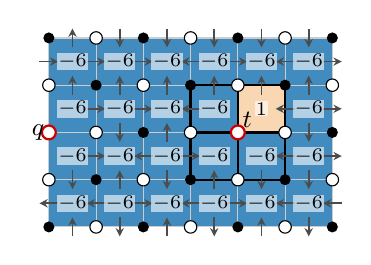
\begin{tikzpicture}[scale=0.6]
\fill[pcA!85] (0,0) rectangle (1,1);
\fill[pcA!85] (0,1) rectangle (1,2);
\fill[pcA!85] (0,2) rectangle (1,3);
\fill[pcA!85] (0,3) rectangle (1,4);
\fill[pcA!85] (1,0) rectangle (2,1);
\fill[pcA!85] (1,1) rectangle (2,2);
\fill[pcA!85] (1,2) rectangle (2,3);
\fill[pcA!85] (1,3) rectangle (2,4);
\fill[pcA!85] (2,0) rectangle (3,1);
\fill[pcA!85] (2,1) rectangle (3,2);
\fill[pcA!85] (2,2) rectangle (3,3);
\fill[pcA!85] (2,3) rectangle (3,4);
\fill[pcA!85] (3,0) rectangle (4,1);
\fill[pcA!85] (3,1) rectangle (4,2);
\fill[pcA!85] (3,2) rectangle (4,3);
\fill[pcA!85] (3,3) rectangle (4,4);
\fill[pcA!85] (4,0) rectangle (5,1);
\fill[pcA!85] (4,1) rectangle (5,2);
\fill[orng!30] (4,2) rectangle (5,3);
\fill[pcA!85] (4,3) rectangle (5,4);
\fill[pcA!85] (5,0) rectangle (6,1);
\fill[pcA!85] (5,1) rectangle (6,2);
\fill[pcA!85] (5,2) rectangle (6,3);
\fill[pcA!85] (5,3) rectangle (6,4);
\draw[gray!40] (0,0) grid (6,4);
\draw[black,thick] (3,1) rectangle (4,2);
\draw[black,thick] (4,1) rectangle (5,2);
\draw[black,thick] (3,2) rectangle (4,3);
\draw[black,thick] (4,2) rectangle (5,3);
\draw[arcarrowsm] (0.20,0.50) -- (-0.20,0.50);
\draw[arcarrowsm] (-0.20,3.50) -- (0.20,3.50);
\draw[arcarrowsm] (0.50,-0.20) -- (0.50,0.20);
\draw[arcarrowsm] (0.50,1.20) -- (0.50,0.80);
\draw[arcarrowsm] (1.20,0.50) -- (0.80,0.50);
\draw[arcarrowsm] (0.80,1.50) -- (1.20,1.50);
\draw[arcarrowsm] (0.50,2.80) -- (0.50,3.20);
\draw[arcarrowsm] (0.80,2.50) -- (1.20,2.50);
\draw[arcarrowsm] (0.50,3.80) -- (0.50,4.20);
\draw[arcarrowsm] (0.80,3.50) -- (1.20,3.50);
\draw[arcarrowsm] (1.50,0.20) -- (1.50,-0.20);
\draw[arcarrowsm] (1.50,0.80) -- (1.50,1.20);
\draw[arcarrowsm] (1.80,0.50) -- (2.20,0.50);
\draw[arcarrowsm] (1.50,2.20) -- (1.50,1.80);
\draw[arcarrowsm] (2.20,1.50) -- (1.80,1.50);
\draw[arcarrowsm] (1.50,2.80) -- (1.50,3.20);
\draw[arcarrowsm] (1.80,2.50) -- (2.20,2.50);
\draw[arcarrowsm] (1.50,4.20) -- (1.50,3.80);
\draw[arcarrowsm] (1.80,3.50) -- (2.20,3.50);
\draw[arcarrowsm] (2.50,-0.20) -- (2.50,0.20);
\draw[arcarrowsm] (2.50,1.20) -- (2.50,0.80);
\draw[arcarrowsm] (3.20,0.50) -- (2.80,0.50);
\draw[arcarrowsm] (2.50,1.80) -- (2.50,2.20);
\draw[arcarrowsm] (2.80,1.50) -- (3.20,1.50);
\draw[arcarrowsm] (2.50,2.80) -- (2.50,3.20);
\draw[arcarrowsm] (3.20,2.50) -- (2.80,2.50);
\draw[arcarrowsm] (2.50,4.20) -- (2.50,3.80);
\draw[arcarrowsm] (3.20,3.50) -- (2.80,3.50);
\draw[arcarrowsm] (3.50,0.20) -- (3.50,-0.20);
\draw[arcarrowsm] (3.50,0.80) -- (3.50,1.20);
\draw[arcarrowsm] (3.80,0.50) -- (4.20,0.50);
\draw[arcarrowsm] (3.50,2.80) -- (3.50,3.20);
\draw[arcarrowsm] (3.50,4.20) -- (3.50,3.80);
\draw[arcarrowsm] (3.80,3.50) -- (4.20,3.50);
\draw[arcarrowsm] (4.50,-0.20) -- (4.50,0.20);
\draw[arcarrowsm] (4.50,1.20) -- (4.50,0.80);
\draw[arcarrowsm] (5.20,0.50) -- (4.80,0.50);
\draw[arcarrowsm] (5.20,1.50) -- (4.80,1.50);
\draw[arcarrowsm] (4.50,2.80) -- (4.50,3.20);
\draw[arcarrowsm] (5.20,2.50) -- (4.80,2.50);
\draw[arcarrowsm] (4.50,4.20) -- (4.50,3.80);
\draw[arcarrowsm] (5.20,3.50) -- (4.80,3.50);
\draw[arcarrowsm] (5.50,0.20) -- (5.50,-0.20);
\draw[arcarrowsm] (5.50,1.20) -- (5.50,0.80);
\draw[arcarrowsm] (6.20,0.50) -- (5.80,0.50);
\draw[arcarrowsm] (5.50,2.20) -- (5.50,1.80);
\draw[arcarrowsm] (5.80,1.50) -- (6.20,1.50);
\draw[arcarrowsm] (5.50,2.80) -- (5.50,3.20);
\draw[arcarrowsm] (5.80,2.50) -- (6.20,2.50);
\draw[arcarrowsm] (5.50,4.20) -- (5.50,3.80);
\draw[arcarrowsm] (5.80,3.50) -- (6.20,3.50);
\node[font=\scriptsize,fill=white,fill opacity=0.6,text opacity=1,inner sep=0.5pt] at (0+0.5,0+0.5) {$-6$};
\node[font=\scriptsize,fill=white,fill opacity=0.6,text opacity=1,inner sep=0.5pt] at (0+0.5,1+0.5) {$-6$};
\node[font=\scriptsize,fill=white,fill opacity=0.6,text opacity=1,inner sep=0.5pt] at (0+0.5,2+0.5) {$-6$};
\node[font=\scriptsize,fill=white,fill opacity=0.6,text opacity=1,inner sep=0.5pt] at (0+0.5,3+0.5) {$-6$};
\node[font=\scriptsize,fill=white,fill opacity=0.6,text opacity=1,inner sep=0.5pt] at (1+0.5,0+0.5) {$-6$};
\node[font=\scriptsize,fill=white,fill opacity=0.6,text opacity=1,inner sep=0.5pt] at (1+0.5,1+0.5) {$-6$};
\node[font=\scriptsize,fill=white,fill opacity=0.6,text opacity=1,inner sep=0.5pt] at (1+0.5,2+0.5) {$-6$};
\node[font=\scriptsize,fill=white,fill opacity=0.6,text opacity=1,inner sep=0.5pt] at (1+0.5,3+0.5) {$-6$};
\node[font=\scriptsize,fill=white,fill opacity=0.6,text opacity=1,inner sep=0.5pt] at (2+0.5,0+0.5) {$-6$};
\node[font=\scriptsize,fill=white,fill opacity=0.6,text opacity=1,inner sep=0.5pt] at (2+0.5,1+0.5) {$-6$};
\node[font=\scriptsize,fill=white,fill opacity=0.6,text opacity=1,inner sep=0.5pt] at (2+0.5,2+0.5) {$-6$};
\node[font=\scriptsize,fill=white,fill opacity=0.6,text opacity=1,inner sep=0.5pt] at (2+0.5,3+0.5) {$-6$};
\node[font=\scriptsize,fill=white,fill opacity=0.6,text opacity=1,inner sep=0.5pt] at (3+0.5,0+0.5) {$-6$};
\node[font=\scriptsize,fill=white,fill opacity=0.6,text opacity=1,inner sep=0.5pt] at (3+0.5,1+0.5) {$-6$};
\node[font=\scriptsize,fill=white,fill opacity=0.6,text opacity=1,inner sep=0.5pt] at (3+0.5,2+0.5) {$-6$};
\node[font=\scriptsize,fill=white,fill opacity=0.6,text opacity=1,inner sep=0.5pt] at (3+0.5,3+0.5) {$-6$};
\node[font=\scriptsize,fill=white,fill opacity=0.6,text opacity=1,inner sep=0.5pt] at (4+0.5,0+0.5) {$-6$};
\node[font=\scriptsize,fill=white,fill opacity=0.6,text opacity=1,inner sep=0.5pt] at (4+0.5,1+0.5) {$-6$};
\node[font=\scriptsize,fill=white,fill opacity=0.6,text opacity=1,inner sep=0.5pt] at (4+0.5,2+0.5) {$1$};
\node[font=\scriptsize,fill=white,fill opacity=0.6,text opacity=1,inner sep=0.5pt] at (4+0.5,3+0.5) {$-6$};
\node[font=\scriptsize,fill=white,fill opacity=0.6,text opacity=1,inner sep=0.5pt] at (5+0.5,0+0.5) {$-6$};
\node[font=\scriptsize,fill=white,fill opacity=0.6,text opacity=1,inner sep=0.5pt] at (5+0.5,1+0.5) {$-6$};
\node[font=\scriptsize,fill=white,fill opacity=0.6,text opacity=1,inner sep=0.5pt] at (5+0.5,2+0.5) {$-6$};
\node[font=\scriptsize,fill=white,fill opacity=0.6,text opacity=1,inner sep=0.5pt] at (5+0.5,3+0.5) {$-6$};
\node[pt] at (0,0) {};
\node[wpt] at (0,1) {};
\node[wpt] at (0,3) {};
\node[pt] at (0,4) {};
\node[wpt] at (1,0) {};
\node[pt] at (1,1) {};
\node[wpt] at (1,2) {};
\node[pt] at (1,3) {};
\node[wpt] at (1,4) {};
\node[pt] at (2,0) {};
\node[wpt] at (2,1) {};
\node[pt] at (2,2) {};
\node[wpt] at (2,3) {};
\node[pt] at (2,4) {};
\node[wpt] at (3,0) {};
\node[pt] at (3,1) {};
\node[wpt] at (3,2) {};
\node[pt] at (3,3) {};
\node[wpt] at (3,4) {};
\node[pt] at (4,0) {};
\node[wpt] at (4,1) {};
\node[wpt] at (4,3) {};
\node[pt] at (4,4) {};
\node[wpt] at (5,0) {};
\node[pt] at (5,1) {};
\node[wpt] at (5,2) {};
\node[pt] at (5,3) {};
\node[wpt] at (5,4) {};
\node[pt] at (6,0) {};
\node[wpt] at (6,1) {};
\node[pt] at (6,2) {};
\node[wpt] at (6,3) {};
\node[pt] at (6,4) {};
\node[miss] at (0,2) {};
\node[miss] at (4,2) {};
\node[lab,above right] at (4,2) {$t$};
\node[lab,left] at (0,2) {$q$};
\end{tikzpicture} & 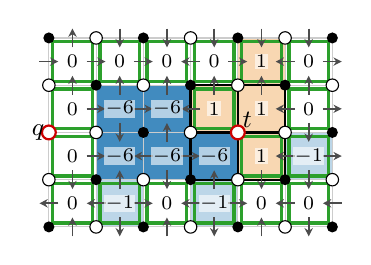
\begin{tikzpicture}[scale=0.6]
\fill[pcA!30] (1,0) rectangle (2,1);
\fill[pcA!85] (1,1) rectangle (2,2);
\fill[pcA!85] (1,2) rectangle (2,3);
\fill[pcA!85] (2,1) rectangle (3,2);
\fill[pcA!85] (2,2) rectangle (3,3);
\fill[pcA!30] (3,0) rectangle (4,1);
\fill[pcA!85] (3,1) rectangle (4,2);
\fill[orng!30] (3,2) rectangle (4,3);
\fill[orng!30] (4,1) rectangle (5,2);
\fill[orng!30] (4,2) rectangle (5,3);
\fill[orng!30] (4,3) rectangle (5,4);
\fill[pcA!30] (5,1) rectangle (6,2);
\draw[gray!40] (0,0) grid (6,4);
\draw[black,thick] (3,1) rectangle (4,2);
\draw[black,thick] (4,1) rectangle (5,2);
\draw[black,thick] (3,2) rectangle (4,3);
\draw[black,thick] (4,2) rectangle (5,3);
\draw[pcC,very thick] (0.08,0.08) rectangle (0.92,0.92);
\draw[pcC,very thick] (0.08,1.08) rectangle (0.92,1.92);
\draw[pcC,very thick] (0.08,2.08) rectangle (0.92,2.92);
\draw[pcC,very thick] (0.08,3.08) rectangle (0.92,3.92);
\draw[pcC,very thick] (1.08,0.08) rectangle (1.92,0.92);
\draw[pcC,very thick] (1.08,3.08) rectangle (1.92,3.92);
\draw[pcC,very thick] (2.08,0.08) rectangle (2.92,0.92);
\draw[pcC,very thick] (2.08,3.08) rectangle (2.92,3.92);
\draw[pcC,very thick] (3.08,0.08) rectangle (3.92,0.92);
\draw[pcC,very thick] (3.08,2.08) rectangle (3.92,2.92);
\draw[pcC,very thick] (3.08,3.08) rectangle (3.92,3.92);
\draw[pcC,very thick] (4.08,0.08) rectangle (4.92,0.92);
\draw[pcC,very thick] (4.08,1.08) rectangle (4.92,1.92);
\draw[pcC,very thick] (4.08,3.08) rectangle (4.92,3.92);
\draw[pcC,very thick] (5.08,0.08) rectangle (5.92,0.92);
\draw[pcC,very thick] (5.08,1.08) rectangle (5.92,1.92);
\draw[pcC,very thick] (5.08,2.08) rectangle (5.92,2.92);
\draw[pcC,very thick] (5.08,3.08) rectangle (5.92,3.92);
\draw[arcarrowsm] (0.20,0.50) -- (-0.20,0.50);
\draw[arcarrowsm] (-0.20,3.50) -- (0.20,3.50);
\draw[arcarrowsm] (0.50,-0.20) -- (0.50,0.20);
\draw[arcarrowsm] (0.50,1.20) -- (0.50,0.80);
\draw[arcarrowsm] (1.20,0.50) -- (0.80,0.50);
\draw[arcarrowsm] (0.80,1.50) -- (1.20,1.50);
\draw[arcarrowsm] (0.50,2.80) -- (0.50,3.20);
\draw[arcarrowsm] (0.80,2.50) -- (1.20,2.50);
\draw[arcarrowsm] (0.50,3.80) -- (0.50,4.20);
\draw[arcarrowsm] (0.80,3.50) -- (1.20,3.50);
\draw[arcarrowsm] (1.50,0.20) -- (1.50,-0.20);
\draw[arcarrowsm] (1.50,0.80) -- (1.50,1.20);
\draw[arcarrowsm] (1.80,0.50) -- (2.20,0.50);
\draw[arcarrowsm] (1.50,2.20) -- (1.50,1.80);
\draw[arcarrowsm] (2.20,1.50) -- (1.80,1.50);
\draw[arcarrowsm] (1.50,2.80) -- (1.50,3.20);
\draw[arcarrowsm] (1.80,2.50) -- (2.20,2.50);
\draw[arcarrowsm] (1.50,4.20) -- (1.50,3.80);
\draw[arcarrowsm] (1.80,3.50) -- (2.20,3.50);
\draw[arcarrowsm] (2.50,-0.20) -- (2.50,0.20);
\draw[arcarrowsm] (2.50,1.20) -- (2.50,0.80);
\draw[arcarrowsm] (3.20,0.50) -- (2.80,0.50);
\draw[arcarrowsm] (2.50,1.80) -- (2.50,2.20);
\draw[arcarrowsm] (2.80,1.50) -- (3.20,1.50);
\draw[arcarrowsm] (2.50,2.80) -- (2.50,3.20);
\draw[arcarrowsm] (3.20,2.50) -- (2.80,2.50);
\draw[arcarrowsm] (2.50,4.20) -- (2.50,3.80);
\draw[arcarrowsm] (3.20,3.50) -- (2.80,3.50);
\draw[arcarrowsm] (3.50,0.20) -- (3.50,-0.20);
\draw[arcarrowsm] (3.50,0.80) -- (3.50,1.20);
\draw[arcarrowsm] (3.80,0.50) -- (4.20,0.50);
\draw[arcarrowsm] (3.50,2.80) -- (3.50,3.20);
\draw[arcarrowsm] (3.50,4.20) -- (3.50,3.80);
\draw[arcarrowsm] (3.80,3.50) -- (4.20,3.50);
\draw[arcarrowsm] (4.50,-0.20) -- (4.50,0.20);
\draw[arcarrowsm] (4.50,1.20) -- (4.50,0.80);
\draw[arcarrowsm] (5.20,0.50) -- (4.80,0.50);
\draw[arcarrowsm] (5.20,1.50) -- (4.80,1.50);
\draw[arcarrowsm] (4.50,2.80) -- (4.50,3.20);
\draw[arcarrowsm] (5.20,2.50) -- (4.80,2.50);
\draw[arcarrowsm] (4.50,4.20) -- (4.50,3.80);
\draw[arcarrowsm] (5.20,3.50) -- (4.80,3.50);
\draw[arcarrowsm] (5.50,0.20) -- (5.50,-0.20);
\draw[arcarrowsm] (5.50,1.20) -- (5.50,0.80);
\draw[arcarrowsm] (6.20,0.50) -- (5.80,0.50);
\draw[arcarrowsm] (5.50,2.20) -- (5.50,1.80);
\draw[arcarrowsm] (5.80,1.50) -- (6.20,1.50);
\draw[arcarrowsm] (5.50,2.80) -- (5.50,3.20);
\draw[arcarrowsm] (5.80,2.50) -- (6.20,2.50);
\draw[arcarrowsm] (5.50,4.20) -- (5.50,3.80);
\draw[arcarrowsm] (5.80,3.50) -- (6.20,3.50);
\node[font=\scriptsize,fill=white,fill opacity=0.6,text opacity=1,inner sep=0.5pt] at (0+0.5,0+0.5) {$0$};
\node[font=\scriptsize,fill=white,fill opacity=0.6,text opacity=1,inner sep=0.5pt] at (0+0.5,1+0.5) {$0$};
\node[font=\scriptsize,fill=white,fill opacity=0.6,text opacity=1,inner sep=0.5pt] at (0+0.5,2+0.5) {$0$};
\node[font=\scriptsize,fill=white,fill opacity=0.6,text opacity=1,inner sep=0.5pt] at (0+0.5,3+0.5) {$0$};
\node[font=\scriptsize,fill=white,fill opacity=0.6,text opacity=1,inner sep=0.5pt] at (1+0.5,0+0.5) {$-1$};
\node[font=\scriptsize,fill=white,fill opacity=0.6,text opacity=1,inner sep=0.5pt] at (1+0.5,1+0.5) {$-6$};
\node[font=\scriptsize,fill=white,fill opacity=0.6,text opacity=1,inner sep=0.5pt] at (1+0.5,2+0.5) {$-6$};
\node[font=\scriptsize,fill=white,fill opacity=0.6,text opacity=1,inner sep=0.5pt] at (1+0.5,3+0.5) {$0$};
\node[font=\scriptsize,fill=white,fill opacity=0.6,text opacity=1,inner sep=0.5pt] at (2+0.5,0+0.5) {$0$};
\node[font=\scriptsize,fill=white,fill opacity=0.6,text opacity=1,inner sep=0.5pt] at (2+0.5,1+0.5) {$-6$};
\node[font=\scriptsize,fill=white,fill opacity=0.6,text opacity=1,inner sep=0.5pt] at (2+0.5,2+0.5) {$-6$};
\node[font=\scriptsize,fill=white,fill opacity=0.6,text opacity=1,inner sep=0.5pt] at (2+0.5,3+0.5) {$0$};
\node[font=\scriptsize,fill=white,fill opacity=0.6,text opacity=1,inner sep=0.5pt] at (3+0.5,0+0.5) {$-1$};
\node[font=\scriptsize,fill=white,fill opacity=0.6,text opacity=1,inner sep=0.5pt] at (3+0.5,1+0.5) {$-6$};
\node[font=\scriptsize,fill=white,fill opacity=0.6,text opacity=1,inner sep=0.5pt] at (3+0.5,2+0.5) {$1$};
\node[font=\scriptsize,fill=white,fill opacity=0.6,text opacity=1,inner sep=0.5pt] at (3+0.5,3+0.5) {$0$};
\node[font=\scriptsize,fill=white,fill opacity=0.6,text opacity=1,inner sep=0.5pt] at (4+0.5,0+0.5) {$0$};
\node[font=\scriptsize,fill=white,fill opacity=0.6,text opacity=1,inner sep=0.5pt] at (4+0.5,1+0.5) {$1$};
\node[font=\scriptsize,fill=white,fill opacity=0.6,text opacity=1,inner sep=0.5pt] at (4+0.5,2+0.5) {$1$};
\node[font=\scriptsize,fill=white,fill opacity=0.6,text opacity=1,inner sep=0.5pt] at (4+0.5,3+0.5) {$1$};
\node[font=\scriptsize,fill=white,fill opacity=0.6,text opacity=1,inner sep=0.5pt] at (5+0.5,0+0.5) {$0$};
\node[font=\scriptsize,fill=white,fill opacity=0.6,text opacity=1,inner sep=0.5pt] at (5+0.5,1+0.5) {$-1$};
\node[font=\scriptsize,fill=white,fill opacity=0.6,text opacity=1,inner sep=0.5pt] at (5+0.5,2+0.5) {$0$};
\node[font=\scriptsize,fill=white,fill opacity=0.6,text opacity=1,inner sep=0.5pt] at (5+0.5,3+0.5) {$0$};
\node[pt] at (0,0) {};
\node[wpt] at (0,1) {};
\node[wpt] at (0,3) {};
\node[pt] at (0,4) {};
\node[wpt] at (1,0) {};
\node[pt] at (1,1) {};
\node[wpt] at (1,2) {};
\node[pt] at (1,3) {};
\node[wpt] at (1,4) {};
\node[pt] at (2,0) {};
\node[wpt] at (2,1) {};
\node[pt] at (2,2) {};
\node[wpt] at (2,3) {};
\node[pt] at (2,4) {};
\node[wpt] at (3,0) {};
\node[pt] at (3,1) {};
\node[wpt] at (3,2) {};
\node[pt] at (3,3) {};
\node[wpt] at (3,4) {};
\node[pt] at (4,0) {};
\node[wpt] at (4,1) {};
\node[wpt] at (4,3) {};
\node[pt] at (4,4) {};
\node[wpt] at (5,0) {};
\node[pt] at (5,1) {};
\node[wpt] at (5,2) {};
\node[pt] at (5,3) {};
\node[wpt] at (5,4) {};
\node[pt] at (6,0) {};
\node[wpt] at (6,1) {};
\node[pt] at (6,2) {};
\node[wpt] at (6,3) {};
\node[pt] at (6,4) {};
\node[miss] at (0,2) {};
\node[miss] at (4,2) {};
\node[lab,above right] at (4,2) {$t$};
\node[lab,left] at (0,2) {$q$};
\end{tikzpicture} \\
\small (f) start & \small (g) round 1
\end{tabular}\\[6pt]
\begin{tabular}{c@{\quad}c}
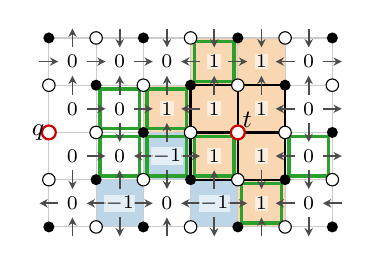
\begin{tikzpicture}[scale=0.6]
\fill[pcA!30] (1,0) rectangle (2,1);
\fill[pcA!30] (2,1) rectangle (3,2);
\fill[orng!30] (2,2) rectangle (3,3);
\fill[pcA!30] (3,0) rectangle (4,1);
\fill[orng!30] (3,1) rectangle (4,2);
\fill[orng!30] (3,2) rectangle (4,3);
\fill[orng!30] (3,3) rectangle (4,4);
\fill[orng!30] (4,0) rectangle (5,1);
\fill[orng!30] (4,1) rectangle (5,2);
\fill[orng!30] (4,2) rectangle (5,3);
\fill[orng!30] (4,3) rectangle (5,4);
\draw[gray!40] (0,0) grid (6,4);
\draw[black,thick] (3,1) rectangle (4,2);
\draw[black,thick] (4,1) rectangle (5,2);
\draw[black,thick] (3,2) rectangle (4,3);
\draw[black,thick] (4,2) rectangle (5,3);
\draw[pcC,very thick] (1.08,1.08) rectangle (1.92,1.92);
\draw[pcC,very thick] (1.08,2.08) rectangle (1.92,2.92);
\draw[pcC,very thick] (2.08,1.08) rectangle (2.92,1.92);
\draw[pcC,very thick] (2.08,2.08) rectangle (2.92,2.92);
\draw[pcC,very thick] (3.08,1.08) rectangle (3.92,1.92);
\draw[pcC,very thick] (3.08,3.08) rectangle (3.92,3.92);
\draw[pcC,very thick] (4.08,0.08) rectangle (4.92,0.92);
\draw[pcC,very thick] (5.08,1.08) rectangle (5.92,1.92);
\draw[arcarrowsm] (0.20,0.50) -- (-0.20,0.50);
\draw[arcarrowsm] (-0.20,3.50) -- (0.20,3.50);
\draw[arcarrowsm] (0.50,-0.20) -- (0.50,0.20);
\draw[arcarrowsm] (0.50,1.20) -- (0.50,0.80);
\draw[arcarrowsm] (1.20,0.50) -- (0.80,0.50);
\draw[arcarrowsm] (0.80,1.50) -- (1.20,1.50);
\draw[arcarrowsm] (0.50,2.80) -- (0.50,3.20);
\draw[arcarrowsm] (0.80,2.50) -- (1.20,2.50);
\draw[arcarrowsm] (0.50,3.80) -- (0.50,4.20);
\draw[arcarrowsm] (0.80,3.50) -- (1.20,3.50);
\draw[arcarrowsm] (1.50,0.20) -- (1.50,-0.20);
\draw[arcarrowsm] (1.50,0.80) -- (1.50,1.20);
\draw[arcarrowsm] (1.80,0.50) -- (2.20,0.50);
\draw[arcarrowsm] (1.50,2.20) -- (1.50,1.80);
\draw[arcarrowsm] (2.20,1.50) -- (1.80,1.50);
\draw[arcarrowsm] (1.50,2.80) -- (1.50,3.20);
\draw[arcarrowsm] (1.80,2.50) -- (2.20,2.50);
\draw[arcarrowsm] (1.50,4.20) -- (1.50,3.80);
\draw[arcarrowsm] (1.80,3.50) -- (2.20,3.50);
\draw[arcarrowsm] (2.50,-0.20) -- (2.50,0.20);
\draw[arcarrowsm] (2.50,1.20) -- (2.50,0.80);
\draw[arcarrowsm] (3.20,0.50) -- (2.80,0.50);
\draw[arcarrowsm] (2.50,1.80) -- (2.50,2.20);
\draw[arcarrowsm] (2.80,1.50) -- (3.20,1.50);
\draw[arcarrowsm] (2.50,2.80) -- (2.50,3.20);
\draw[arcarrowsm] (3.20,2.50) -- (2.80,2.50);
\draw[arcarrowsm] (2.50,4.20) -- (2.50,3.80);
\draw[arcarrowsm] (3.20,3.50) -- (2.80,3.50);
\draw[arcarrowsm] (3.50,0.20) -- (3.50,-0.20);
\draw[arcarrowsm] (3.50,0.80) -- (3.50,1.20);
\draw[arcarrowsm] (3.80,0.50) -- (4.20,0.50);
\draw[arcarrowsm] (3.50,2.80) -- (3.50,3.20);
\draw[arcarrowsm] (3.50,4.20) -- (3.50,3.80);
\draw[arcarrowsm] (3.80,3.50) -- (4.20,3.50);
\draw[arcarrowsm] (4.50,-0.20) -- (4.50,0.20);
\draw[arcarrowsm] (4.50,1.20) -- (4.50,0.80);
\draw[arcarrowsm] (5.20,0.50) -- (4.80,0.50);
\draw[arcarrowsm] (5.20,1.50) -- (4.80,1.50);
\draw[arcarrowsm] (4.50,2.80) -- (4.50,3.20);
\draw[arcarrowsm] (5.20,2.50) -- (4.80,2.50);
\draw[arcarrowsm] (4.50,4.20) -- (4.50,3.80);
\draw[arcarrowsm] (5.20,3.50) -- (4.80,3.50);
\draw[arcarrowsm] (5.50,0.20) -- (5.50,-0.20);
\draw[arcarrowsm] (5.50,1.20) -- (5.50,0.80);
\draw[arcarrowsm] (6.20,0.50) -- (5.80,0.50);
\draw[arcarrowsm] (5.50,2.20) -- (5.50,1.80);
\draw[arcarrowsm] (5.80,1.50) -- (6.20,1.50);
\draw[arcarrowsm] (5.50,2.80) -- (5.50,3.20);
\draw[arcarrowsm] (5.80,2.50) -- (6.20,2.50);
\draw[arcarrowsm] (5.50,4.20) -- (5.50,3.80);
\draw[arcarrowsm] (5.80,3.50) -- (6.20,3.50);
\node[font=\scriptsize,fill=white,fill opacity=0.6,text opacity=1,inner sep=0.5pt] at (0+0.5,0+0.5) {$0$};
\node[font=\scriptsize,fill=white,fill opacity=0.6,text opacity=1,inner sep=0.5pt] at (0+0.5,1+0.5) {$0$};
\node[font=\scriptsize,fill=white,fill opacity=0.6,text opacity=1,inner sep=0.5pt] at (0+0.5,2+0.5) {$0$};
\node[font=\scriptsize,fill=white,fill opacity=0.6,text opacity=1,inner sep=0.5pt] at (0+0.5,3+0.5) {$0$};
\node[font=\scriptsize,fill=white,fill opacity=0.6,text opacity=1,inner sep=0.5pt] at (1+0.5,0+0.5) {$-1$};
\node[font=\scriptsize,fill=white,fill opacity=0.6,text opacity=1,inner sep=0.5pt] at (1+0.5,1+0.5) {$0$};
\node[font=\scriptsize,fill=white,fill opacity=0.6,text opacity=1,inner sep=0.5pt] at (1+0.5,2+0.5) {$0$};
\node[font=\scriptsize,fill=white,fill opacity=0.6,text opacity=1,inner sep=0.5pt] at (1+0.5,3+0.5) {$0$};
\node[font=\scriptsize,fill=white,fill opacity=0.6,text opacity=1,inner sep=0.5pt] at (2+0.5,0+0.5) {$0$};
\node[font=\scriptsize,fill=white,fill opacity=0.6,text opacity=1,inner sep=0.5pt] at (2+0.5,1+0.5) {$-1$};
\node[font=\scriptsize,fill=white,fill opacity=0.6,text opacity=1,inner sep=0.5pt] at (2+0.5,2+0.5) {$1$};
\node[font=\scriptsize,fill=white,fill opacity=0.6,text opacity=1,inner sep=0.5pt] at (2+0.5,3+0.5) {$0$};
\node[font=\scriptsize,fill=white,fill opacity=0.6,text opacity=1,inner sep=0.5pt] at (3+0.5,0+0.5) {$-1$};
\node[font=\scriptsize,fill=white,fill opacity=0.6,text opacity=1,inner sep=0.5pt] at (3+0.5,1+0.5) {$1$};
\node[font=\scriptsize,fill=white,fill opacity=0.6,text opacity=1,inner sep=0.5pt] at (3+0.5,2+0.5) {$1$};
\node[font=\scriptsize,fill=white,fill opacity=0.6,text opacity=1,inner sep=0.5pt] at (3+0.5,3+0.5) {$1$};
\node[font=\scriptsize,fill=white,fill opacity=0.6,text opacity=1,inner sep=0.5pt] at (4+0.5,0+0.5) {$1$};
\node[font=\scriptsize,fill=white,fill opacity=0.6,text opacity=1,inner sep=0.5pt] at (4+0.5,1+0.5) {$1$};
\node[font=\scriptsize,fill=white,fill opacity=0.6,text opacity=1,inner sep=0.5pt] at (4+0.5,2+0.5) {$1$};
\node[font=\scriptsize,fill=white,fill opacity=0.6,text opacity=1,inner sep=0.5pt] at (4+0.5,3+0.5) {$1$};
\node[font=\scriptsize,fill=white,fill opacity=0.6,text opacity=1,inner sep=0.5pt] at (5+0.5,0+0.5) {$0$};
\node[font=\scriptsize,fill=white,fill opacity=0.6,text opacity=1,inner sep=0.5pt] at (5+0.5,1+0.5) {$0$};
\node[font=\scriptsize,fill=white,fill opacity=0.6,text opacity=1,inner sep=0.5pt] at (5+0.5,2+0.5) {$0$};
\node[font=\scriptsize,fill=white,fill opacity=0.6,text opacity=1,inner sep=0.5pt] at (5+0.5,3+0.5) {$0$};
\node[pt] at (0,0) {};
\node[wpt] at (0,1) {};
\node[wpt] at (0,3) {};
\node[pt] at (0,4) {};
\node[wpt] at (1,0) {};
\node[pt] at (1,1) {};
\node[wpt] at (1,2) {};
\node[pt] at (1,3) {};
\node[wpt] at (1,4) {};
\node[pt] at (2,0) {};
\node[wpt] at (2,1) {};
\node[pt] at (2,2) {};
\node[wpt] at (2,3) {};
\node[pt] at (2,4) {};
\node[wpt] at (3,0) {};
\node[pt] at (3,1) {};
\node[wpt] at (3,2) {};
\node[pt] at (3,3) {};
\node[wpt] at (3,4) {};
\node[pt] at (4,0) {};
\node[wpt] at (4,1) {};
\node[wpt] at (4,3) {};
\node[pt] at (4,4) {};
\node[wpt] at (5,0) {};
\node[pt] at (5,1) {};
\node[wpt] at (5,2) {};
\node[pt] at (5,3) {};
\node[wpt] at (5,4) {};
\node[pt] at (6,0) {};
\node[wpt] at (6,1) {};
\node[pt] at (6,2) {};
\node[wpt] at (6,3) {};
\node[pt] at (6,4) {};
\node[miss] at (0,2) {};
\node[miss] at (4,2) {};
\node[lab,above right] at (4,2) {$t$};
\node[lab,left] at (0,2) {$q$};
\end{tikzpicture} & 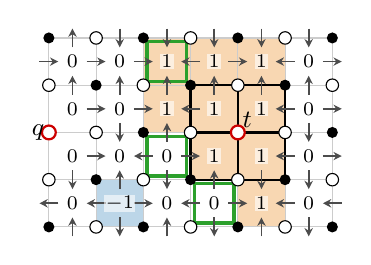
\begin{tikzpicture}[scale=0.6]
\fill[pcA!30] (1,0) rectangle (2,1);
\fill[orng!30] (2,2) rectangle (3,3);
\fill[orng!30] (2,3) rectangle (3,4);
\fill[orng!30] (3,1) rectangle (4,2);
\fill[orng!30] (3,2) rectangle (4,3);
\fill[orng!30] (3,3) rectangle (4,4);
\fill[orng!30] (4,0) rectangle (5,1);
\fill[orng!30] (4,1) rectangle (5,2);
\fill[orng!30] (4,2) rectangle (5,3);
\fill[orng!30] (4,3) rectangle (5,4);
\draw[gray!40] (0,0) grid (6,4);
\draw[black,thick] (3,1) rectangle (4,2);
\draw[black,thick] (4,1) rectangle (5,2);
\draw[black,thick] (3,2) rectangle (4,3);
\draw[black,thick] (4,2) rectangle (5,3);
\draw[pcC,very thick] (2.08,1.08) rectangle (2.92,1.92);
\draw[pcC,very thick] (2.08,3.08) rectangle (2.92,3.92);
\draw[pcC,very thick] (3.08,0.08) rectangle (3.92,0.92);
\draw[arcarrowsm] (0.20,0.50) -- (-0.20,0.50);
\draw[arcarrowsm] (-0.20,3.50) -- (0.20,3.50);
\draw[arcarrowsm] (0.50,-0.20) -- (0.50,0.20);
\draw[arcarrowsm] (0.50,1.20) -- (0.50,0.80);
\draw[arcarrowsm] (1.20,0.50) -- (0.80,0.50);
\draw[arcarrowsm] (0.80,1.50) -- (1.20,1.50);
\draw[arcarrowsm] (0.50,2.80) -- (0.50,3.20);
\draw[arcarrowsm] (0.80,2.50) -- (1.20,2.50);
\draw[arcarrowsm] (0.50,3.80) -- (0.50,4.20);
\draw[arcarrowsm] (0.80,3.50) -- (1.20,3.50);
\draw[arcarrowsm] (1.50,0.20) -- (1.50,-0.20);
\draw[arcarrowsm] (1.50,0.80) -- (1.50,1.20);
\draw[arcarrowsm] (1.80,0.50) -- (2.20,0.50);
\draw[arcarrowsm] (1.50,2.20) -- (1.50,1.80);
\draw[arcarrowsm] (2.20,1.50) -- (1.80,1.50);
\draw[arcarrowsm] (1.50,2.80) -- (1.50,3.20);
\draw[arcarrowsm] (1.80,2.50) -- (2.20,2.50);
\draw[arcarrowsm] (1.50,4.20) -- (1.50,3.80);
\draw[arcarrowsm] (1.80,3.50) -- (2.20,3.50);
\draw[arcarrowsm] (2.50,-0.20) -- (2.50,0.20);
\draw[arcarrowsm] (2.50,1.20) -- (2.50,0.80);
\draw[arcarrowsm] (3.20,0.50) -- (2.80,0.50);
\draw[arcarrowsm] (2.50,1.80) -- (2.50,2.20);
\draw[arcarrowsm] (2.80,1.50) -- (3.20,1.50);
\draw[arcarrowsm] (2.50,2.80) -- (2.50,3.20);
\draw[arcarrowsm] (3.20,2.50) -- (2.80,2.50);
\draw[arcarrowsm] (2.50,4.20) -- (2.50,3.80);
\draw[arcarrowsm] (3.20,3.50) -- (2.80,3.50);
\draw[arcarrowsm] (3.50,0.20) -- (3.50,-0.20);
\draw[arcarrowsm] (3.50,0.80) -- (3.50,1.20);
\draw[arcarrowsm] (3.80,0.50) -- (4.20,0.50);
\draw[arcarrowsm] (3.50,2.80) -- (3.50,3.20);
\draw[arcarrowsm] (3.50,4.20) -- (3.50,3.80);
\draw[arcarrowsm] (3.80,3.50) -- (4.20,3.50);
\draw[arcarrowsm] (4.50,-0.20) -- (4.50,0.20);
\draw[arcarrowsm] (4.50,1.20) -- (4.50,0.80);
\draw[arcarrowsm] (5.20,0.50) -- (4.80,0.50);
\draw[arcarrowsm] (5.20,1.50) -- (4.80,1.50);
\draw[arcarrowsm] (4.50,2.80) -- (4.50,3.20);
\draw[arcarrowsm] (5.20,2.50) -- (4.80,2.50);
\draw[arcarrowsm] (4.50,4.20) -- (4.50,3.80);
\draw[arcarrowsm] (5.20,3.50) -- (4.80,3.50);
\draw[arcarrowsm] (5.50,0.20) -- (5.50,-0.20);
\draw[arcarrowsm] (5.50,1.20) -- (5.50,0.80);
\draw[arcarrowsm] (6.20,0.50) -- (5.80,0.50);
\draw[arcarrowsm] (5.50,2.20) -- (5.50,1.80);
\draw[arcarrowsm] (5.80,1.50) -- (6.20,1.50);
\draw[arcarrowsm] (5.50,2.80) -- (5.50,3.20);
\draw[arcarrowsm] (5.80,2.50) -- (6.20,2.50);
\draw[arcarrowsm] (5.50,4.20) -- (5.50,3.80);
\draw[arcarrowsm] (5.80,3.50) -- (6.20,3.50);
\node[font=\scriptsize,fill=white,fill opacity=0.6,text opacity=1,inner sep=0.5pt] at (0+0.5,0+0.5) {$0$};
\node[font=\scriptsize,fill=white,fill opacity=0.6,text opacity=1,inner sep=0.5pt] at (0+0.5,1+0.5) {$0$};
\node[font=\scriptsize,fill=white,fill opacity=0.6,text opacity=1,inner sep=0.5pt] at (0+0.5,2+0.5) {$0$};
\node[font=\scriptsize,fill=white,fill opacity=0.6,text opacity=1,inner sep=0.5pt] at (0+0.5,3+0.5) {$0$};
\node[font=\scriptsize,fill=white,fill opacity=0.6,text opacity=1,inner sep=0.5pt] at (1+0.5,0+0.5) {$-1$};
\node[font=\scriptsize,fill=white,fill opacity=0.6,text opacity=1,inner sep=0.5pt] at (1+0.5,1+0.5) {$0$};
\node[font=\scriptsize,fill=white,fill opacity=0.6,text opacity=1,inner sep=0.5pt] at (1+0.5,2+0.5) {$0$};
\node[font=\scriptsize,fill=white,fill opacity=0.6,text opacity=1,inner sep=0.5pt] at (1+0.5,3+0.5) {$0$};
\node[font=\scriptsize,fill=white,fill opacity=0.6,text opacity=1,inner sep=0.5pt] at (2+0.5,0+0.5) {$0$};
\node[font=\scriptsize,fill=white,fill opacity=0.6,text opacity=1,inner sep=0.5pt] at (2+0.5,1+0.5) {$0$};
\node[font=\scriptsize,fill=white,fill opacity=0.6,text opacity=1,inner sep=0.5pt] at (2+0.5,2+0.5) {$1$};
\node[font=\scriptsize,fill=white,fill opacity=0.6,text opacity=1,inner sep=0.5pt] at (2+0.5,3+0.5) {$1$};
\node[font=\scriptsize,fill=white,fill opacity=0.6,text opacity=1,inner sep=0.5pt] at (3+0.5,0+0.5) {$0$};
\node[font=\scriptsize,fill=white,fill opacity=0.6,text opacity=1,inner sep=0.5pt] at (3+0.5,1+0.5) {$1$};
\node[font=\scriptsize,fill=white,fill opacity=0.6,text opacity=1,inner sep=0.5pt] at (3+0.5,2+0.5) {$1$};
\node[font=\scriptsize,fill=white,fill opacity=0.6,text opacity=1,inner sep=0.5pt] at (3+0.5,3+0.5) {$1$};
\node[font=\scriptsize,fill=white,fill opacity=0.6,text opacity=1,inner sep=0.5pt] at (4+0.5,0+0.5) {$1$};
\node[font=\scriptsize,fill=white,fill opacity=0.6,text opacity=1,inner sep=0.5pt] at (4+0.5,1+0.5) {$1$};
\node[font=\scriptsize,fill=white,fill opacity=0.6,text opacity=1,inner sep=0.5pt] at (4+0.5,2+0.5) {$1$};
\node[font=\scriptsize,fill=white,fill opacity=0.6,text opacity=1,inner sep=0.5pt] at (4+0.5,3+0.5) {$1$};
\node[font=\scriptsize,fill=white,fill opacity=0.6,text opacity=1,inner sep=0.5pt] at (5+0.5,0+0.5) {$0$};
\node[font=\scriptsize,fill=white,fill opacity=0.6,text opacity=1,inner sep=0.5pt] at (5+0.5,1+0.5) {$0$};
\node[font=\scriptsize,fill=white,fill opacity=0.6,text opacity=1,inner sep=0.5pt] at (5+0.5,2+0.5) {$0$};
\node[font=\scriptsize,fill=white,fill opacity=0.6,text opacity=1,inner sep=0.5pt] at (5+0.5,3+0.5) {$0$};
\node[pt] at (0,0) {};
\node[wpt] at (0,1) {};
\node[wpt] at (0,3) {};
\node[pt] at (0,4) {};
\node[wpt] at (1,0) {};
\node[pt] at (1,1) {};
\node[wpt] at (1,2) {};
\node[pt] at (1,3) {};
\node[wpt] at (1,4) {};
\node[pt] at (2,0) {};
\node[wpt] at (2,1) {};
\node[pt] at (2,2) {};
\node[wpt] at (2,3) {};
\node[pt] at (2,4) {};
\node[wpt] at (3,0) {};
\node[pt] at (3,1) {};
\node[wpt] at (3,2) {};
\node[pt] at (3,3) {};
\node[wpt] at (3,4) {};
\node[pt] at (4,0) {};
\node[wpt] at (4,1) {};
\node[wpt] at (4,3) {};
\node[pt] at (4,4) {};
\node[wpt] at (5,0) {};
\node[pt] at (5,1) {};
\node[wpt] at (5,2) {};
\node[pt] at (5,3) {};
\node[wpt] at (5,4) {};
\node[pt] at (6,0) {};
\node[wpt] at (6,1) {};
\node[pt] at (6,2) {};
\node[wpt] at (6,3) {};
\node[pt] at (6,4) {};
\node[miss] at (0,2) {};
\node[miss] at (4,2) {};
\node[lab,above right] at (4,2) {$t$};
\node[lab,left] at (0,2) {$q$};
\end{tikzpicture} \\
\small (h) round 2 & \small (i) round 3
\end{tabular}

\caption{The class search on one leaf of the $7\times5$ block, $s=(0,2)$ (deleted, phantom $q$),
inner $t=(4,2)$ (hole cells outlined), branch $w=(3,2)$, $x=(0,3)$.
Every cell shows $\varphi=D(F,G)/2$, orange above $0$ and blue below.
Points are black or white by parity, and the small arrows are the arcs of the reference factor $F$,
which fix the allowed step of $\varphi$ across each side ($0$ or $+1$ along an arrow, $0$ or $-1$
against it).
Sides without an arrow are not edges of $U=V\setminus\{s,t\}$, among them every side at $s$ and
$t$, including the two phantom edges, so $\varphi$ cannot step across them, and the phantom edges
are the same in $F$ and in every factor of the leaf.
(a) The reference factor $F$ from \lean{findFactor}, where $\varphi=0$.
(b)--(d) The least factor of each nonempty class $h=-1,0,1$, with its pieces.
The edge between the plateau and its surroundings is an alternating cycle of $F\oplus G$ around
the hole.
(e) For $h=2$ the numbers are not the heights of a factor.
They are the least values that the value $2$ at the hole forces, and every admissible $\varphi$
with this hole value would be at least as large.
For example, the arrow from the hole cell $(4,2)$ into $(4,3)$ forces $\varphi(4,3)\ge2$, while the
outside square above $(4,3)$ has $\varphi=0$ and the arrow there allows at most $1$.
On the red sides the least values already exceed what the border allows, so no admissible $\varphi$
exists and the class is empty.
(f)--(i) The relaxation for $h=1$.
The prescribed hole cell starts at $1$ and all other squares at $-6$.
Green squares rose in that round.
Round~$3$ is the fixed point, which equals~(d).}
\label{fig:classsearch}
\end{figure}

\begin{theorem}[\lean{classSearchOne\_sound}, \lean{classSearchOne\_complete}, \lean{classSearchOne\_solidFor}, \lean{classSearchOneCost\_le}]
\label{thm:classsearch}
A factor returned by \lean{classSearchOne} has class $h$.
If some factor has class $h$, \lean{classSearchOne} returns a factor $G$ with $\lean{SolidFor}\ U\ G\ G'$ for
every $G'$ of class $h$.
If the bounding box of $U$ has width and height below $|U|$, the cost is at most
$1000(|W|+1)^4$.
\end{theorem}

\begin{proof}
\emph{Factors and potentials.}
Let $G$ have the degrees of $F$ and agree with $F$ off the edges of $U$, and put
$\varphi=D(F,G)/2$.
By the proof of \cref{lem:D}, $\varphi$ jumps across $e$ by the sign of the arc of $F$ when
$e\in F\oplus G$ and by $0$ otherwise.
The squares outside the box form a connected region, and no side between two of them is an edge of
$U$, so $\varphi$ is constant there, and it is $0$ far left.
So $\varphi$ is admissible.
Conversely let $\varphi$ be admissible and $X_\varphi$ the edges of $U$ across which it jumps.
Going once around a point $p$, the jumps of $\varphi$ add up to $0$.
Each jump is $\pm1$ according to the arc of $F$, and going around $p$ the arcs of the dark edges of
$F$ point one way and those of the light edges the other way (\cref{sec:prelim}).
So $X_\varphi$ has as many dark as light edges at $p$, and toggling them keeps the degree of $p$.
Hence $G=F\oplus X_\varphi$ is a factor with the degrees of $F$, and $D(F,G)$ and $2\varphi$ have
the same jumps and are both $0$ far left, so $D(F,G)=2\varphi$.
A factor of class $h$ is therefore the same as an admissible $\varphi$ with $\varphi(t)=h$.

\emph{The relaxation.}
Each inequality between two neighbouring squares gives a lower bound on each of them, of the form
$\varphi(c')\ge\varphi(c)+\beta$.
A round replaces $f(c')$, for every square $c'$ of the box, by the largest such bound when it is
larger, with the squares outside the box fixed at $0$.
After $k$ rounds, $f(c)$ is the largest value of $f_0(c_0)+\beta_1+\dots+\beta_j$ over walks
$c_0,\dots,c_j=c$ with $j\le k$, where $f_0$ is the start.
Suppose an admissible $\psi$ with $\psi(t)=h$ exists.
Then $\psi\ge f_0$, because $\psi\ge-\omega$ everywhere and $\psi(t)=h$.
Adding the inequalities of $\psi$ around a closed walk shows that its $\beta$ add up to at most $0$,
so dropping a closed part of a walk never lowers its value.
Walks of at most $|S|-1$ steps therefore reach every value, where $S$ is the list of squares of the
box, and $f$ is fixed after at most $|S|+1$ rounds, the fuel $\lean{kFuel}$ (\lean{relax\_bf}).
By induction on the rounds, $f\le\psi$.
The fixed point satisfies every lower bound on a square of the box.
The remaining conditions are upper bounds on single squares, namely the bounds that the squares
outside the box, fixed at $0$, put on their neighbours in the box, and $f(t)\le h$.
$\psi$ satisfies them, so $f\le\psi$ does too.
So \lean{isAdmissible} accepts $f$ (\lean{relax\_fix}, \lean{check\_iff}).

\emph{Soundness and completeness.}
If \lean{isAdmissible} accepts the final $f$, then $f$ is admissible with $f(t)=h$, and
$F\oplus X_f$ is a factor of class $h$.
If some factor of class $h$ exists, the previous paragraph shows that the check accepts.
The returned $G$ and every $G'$ of class $h$ have the same class, so \cref{lem:classsolid} gives
$\lean{SolidFor}\ U\ G\ G'$.

\emph{Cost.}
The potentials are stored in an array indexed by box position, so each lookup costs a constant
(\lean{relaxA}, \lean{toFA}), and the array relaxation computes the same values as the relaxation
above (\lean{toFA\_relaxA}, \lean{classPotential\_eq}).
A narrow box has at most $|U|^2$ squares, so $|S|+1$ rounds of $O(|S|)$ work and the check give
the bound.
In general \lean{classSearch} with $k$ prescribed values costs at most $500(k+1)(|W|+1)^4$
(\lean{classSearchCost\_le}).
\end{proof}

The bounding box is \emph{narrow} when its width and height are below $|U|$.
It is narrow whenever a Hamiltonian path exists (\lean{narrow\_of\_ncomp}), and this is
tested first (\lean{isNarrow}).
Classes lie in $[-|U|,|U|]$, because $\varphi$ changes by at most $1$ from one square to the next and
is $0$ outside a narrow box, so the list \lean{classRange} of $2|U|+1$ values covers them.

% =====================================================================
\section{One inner endpoint}
\label{sec:one}

Let $t$ be inner and let $s$ have a missing king neighbour.
The two-phantom core needs the out-vertices $w$ and $s$ Far with phantoms that are not opposed,
and $s$ needs a phantom.
Both come from deletions on the $s$ side (\lean{holeCase}, \lean{holeCaseWalk}, \lean{Algorithm.lean}).
\begin{enumerate}
\item Delete $t$ and branch over its neighbour $w\ne s$ (the last edge of the path).
  The phantom of $w$ is $t$.
\item Delete $s$ and branch over its successor $x\ne w$.
  The new endpoint is $x$, and the deleted $s$ is its phantom $q$.
\item While the current endpoint is within king distance $1$ of $w$, or its phantom $q$ is opposed to
  the phantom $t$ of $w$, delete it again and branch over its successor.
  The phantom $q$ is always the point deleted last.
\item When the endpoint and $w$ are Far and the phantoms are not opposed (\lean{isFar},
  \lean{phantomsOpposed}), run the final test \lean{oneHoleFinalTest}.
  It enumerates classes, calls \lean{classSearchOne}, and runs the two-phantom loop \lean{twoPhantomLoop}.
\end{enumerate}
The measure \lean{wmuG} is the number of points of the current set within king distance $1$ of $w$
(at most $8$), plus $1$ while $q$ is not within king distance $2$ of $w$.
It is at most $9$, and each deletion in step~3 lowers it.
An opposed continuation needs $q$ at king distance $3$ from $w$, which happens only right after
step~2.
So step~3 runs at most $9$ times, and the walk \lean{holeCaseWalk} has fuel $10$.

\paragraph{Why the phantom is the point deleted last.}
Write $r$ for the original $s$, and let $P$ be the path of deleted points from $r$ to $q$.
\Cref{thm:slit} needs degree $2$ at every inner point except the vortex.

\begin{lemma}[\lean{ws\_deg}]
\label{lem:wsdeg}
For every factor $G$ of the current two-phantom setting, $G\cup P$ has degree $1$ at $t$, degree
$1$ at $r$, and degree $2$ at every other inner point of the original $V$.
\end{lemma}

\begin{proof}
The points of the original $V$ are $t$, the points of the current set $U$, and the deleted points,
which are the points of $P$.
A point of $U$ has degree $2$ in $G$, and $P$ has no edge at it.
The point $t$ has degree $1$ in $G$, from its edge $w$--$t$, and is not on $P$.
An inner point of $P$ has degree $2$ in $P$ and no edge of $G$.
The end $q$ of $P$ has one edge in $P$ and one, its phantom edge, in $G$.
The other end $r$ has one edge in $P$ and none in $G$, or, when $P$ is the single point $r=q$, no
edge in $P$ and one in $G$.
\end{proof}

The phantom $q$ gets one edge from $G$ and one from $P$.
If the phantom of the current endpoint were a missing point other than the last deleted one, the
last deleted point would keep degree $1$ in $G\cup P$, and if it were inner it would be a second
vortex.
The point $r$ has a missing king neighbour, so it is not inner.
So $G\cup P$ has the single vortex $t$ on the solid original set.
Its arcs agree with those of $G$ on the cells of the current set, so climbs of $G$ do not close
(\lean{ws\_acyc}, \lean{acyc\_ext}, \cref{thm:vortex}).

\begin{definition}[walk invariant \lean{WS}]
\lean{WS} records the original solid set, the inner $t$, the current set $U$, the current endpoint $s$, its
phantom $q$, the edges $w$--$t$ and $s$--$q$, the deleted path $P$ with the degree condition of
\cref{lem:wsdeg}, and the fact that every missing point of $U$ joins $t$ or $r$ through missing
points or escapes to the left.
\end{definition}

The last field gives \lean{SolidFor} within a class by \cref{lem:classsolid}.
\lean{ws\_init} establishes \lean{WS} after steps~1 and~2, and \lean{ws\_step} keeps it under one
deletion.

\begin{theorem}[\lean{oneHoleCase\_main}, \lean{HoleWalkCost.lean}]
\label{thm:one}
For solid $V$, inner $t$, and $s\ne t$ with a missing king neighbour, \lean{oneHoleCase} decides the
problem within $2\,513\,000\,(|V|+3)^5$ steps.
\end{theorem}

\begin{proof}
By \cref{lem:del}, applied to $t$, to $s$ and to each further deletion, $V$ has a Hamiltonian
$s$--$t$ path exactly when some leaf of the walk has a two-phantom factor with one piece.
The measure \lean{wmuG} bounds the walk, so every branch reaches a leaf within the fuel $10$, and
\lean{WS} holds at every leaf (\lean{ws\_init}, \lean{ws\_step}).
Fix a leaf with current set $U$.
If its box is not narrow, it has no Hamiltonian path (\lean{narrow\_of\_ncomp}) and the answer
\lean{false} is correct.
Otherwise every class lies in \lean{classRange}, and for each class the final test runs
\cref{thm:classsearch} and then the loop from the factor it returns.
Within one class the hypotheses of \cref{sec:sheffield} hold.
Every corner of a cell of $U$ has degree $2$.
By \cref{lem:runclass} every state of the run has the class of its start, so any two factors that
occur are in one class and \cref{lem:classsolid} gives \lean{SolidFor}.
By \cref{lem:wsdeg}, $G\cup P$ has the single vortex $t$ on the original solid set, so by
\cref{thm:vortex} no climb closes, and this passes to $G$ on the cells of $U$ (\lean{ws\_acyc},
\lean{acyc\_ext}).
The walk stops only when $w$ and the current endpoint are Far with phantoms that are not opposed.
So the argument of \cref{thm:twoph} applies within the class.
A stuck phase certifies that no factor of the class has one piece, and otherwise the loop reaches
one piece.
A Hamiltonian path of the leaf lies in some class of \lean{classRange}, so the final test finds it
whenever it exists.
For the cost, the two deletions give $16$ walk starts, each walk makes at most $13$ final tests
(\cref{par:ring}), and each final test costs at most $12\,000\,(|U|+3)^5$.
\end{proof}

% =====================================================================
\section{Two inner endpoints}
\label{sec:two}

When $s$ is inner too, the same walk applies with $r=s$ inner.
Now $G\cup P$ has two vortices, $t$ and $r$.
Two things change.

\paragraph{Classes are pairs.}
The final test \lean{twoHoleFinalTest} enumerates pairs $(h_1,h_2)$ in $\lean{classRange}^2$, at most
$(2|U|+1)^2$ of them, and calls \lean{classSearch} with two prescribed values
(\lean{kFind2\_solidFor}, \lean{HoleTwoV.lean}).

\paragraph{No closed climb with two vortices.}
A single potential of the shape in \cref{thm:vortex} fails.
When one step can change both labels, their changes add up and can cancel the gain of $\tau$.
The fix is to give each vortex a label with three sectors, placed so that no step crosses
boundaries of both.

\begin{theorem}[height with two slits, \lean{height2}, \lean{TwoVortex.lean}]
\label{thm:height2}
Let $V$ be solid, and let $H$ be a factor with degree $1$ at two distinct inner points $v_1,v_2$ and
degree $2$ at every other inner point.
Choose the slits of $v_1$ and $v_2$ as below.
Then there are $\tau$ and $\delta_1,\delta_2\in\{2,-2\}$ such that for every step from a cell $c$ to a
neighbouring cell $c'$
\[\tau(c')-\tau(c)=\varepsilon+\delta_1k_1+\delta_2k_2,\]
where $\varepsilon=+1$ when the arc of $H$ points from $c$ to $c'$ and $-1$ otherwise, and
$k_i\in\{-1,0,1\}$ records a crossing of slit $i$.
For a slit that goes left, $k_i=1$ for an upward crossing and $-1$ for a downward one.
For the slit that goes down, $k_i=1$ for a leftward crossing and $-1$ for a rightward one (Lean
\lean{kL}, \lean{kD}, \lean{tau\_step}).
\end{theorem}

\begin{proof}
As in \cref{app:slit}, with two imbalanced points.
The arcs balance at every inner point except $v_1$ and $v_2$, where they are out of balance by $2$.
A unit flow from $v_i$ along slit $i$ and on to a common far point outside $V$, multiplied by a
suitable $\delta_i\in\{2,-2\}$ and subtracted, removes the imbalance at $v_i$ and moves it to the far
point (\lean{height2}).
The imbalances at points that are not inner are moved there along edges that are not sides between
two cells, which changes no arc between two cells.
The total imbalance is $0$, so afterwards the weights balance at every point and are the jumps of a
function $\tau$.
\end{proof}

The slits are chosen by the relative position of the vortices.
\begin{itemize}
\item \emph{Different rows}, $v_1=(a_1,b_1)$ below $v_2=(a_2,b_2)$.
  Both slits go left along the rows of the vortices.
\item \emph{One row}, $v_1=(a_1,b)$ left of $v_2=(a_2,b)$.
  The slit of $v_1$ goes left along row $b$.
  The slit of $v_2$ goes down along column $a_2$ (Lean \lean{SlitD}).
\end{itemize}

\begin{definition}[three-sector labels]
For a square $c=(x,y)$ define (Lean \lean{labD}, \lean{labU}, \lean{labL}, \lean{labR})
\begin{align*}
\lab_D^{(a,b)}(c)&=\begin{cases}3&y\ge b\\1&y<b,\ x<a\\2&y<b,\ x\ge a\end{cases}&
\lab_U^{(a,b)}(c)&=\begin{cases}1&y<b\\2&y\ge b,\ x\ge a\\3&y\ge b,\ x<a\end{cases}\\
\lab_L^{(a,b)}(c)&=\begin{cases}1&x\ge a\\2&x<a,\ y\ge b\\0&x<a,\ y<b\end{cases}&
\lab_R^{(a,b)}(c)&=\begin{cases}2&x<a\\0&x\ge a,\ y<b\\1&x\ge a,\ y\ge b\end{cases}
\end{align*}
For different rows, $\ell_1=\lab_D^{v_1}$ and $\ell_2=\lab_U^{v_2}$.
For one row, $\ell_1=\lab_L^{v_1}$ and $\ell_2=\lab_R^{v_2}$.
\end{definition}

Each label has three boundary rays from its vortex.
Across its slit it changes by $\pm2$, and across the other two rays by $\pm1$.
\begin{itemize}
\item $\lab_D$: the row $y=b$ (the left part is the slit) and the downward ray $x=a$, $y<b$.
\item $\lab_U$: the row $y=b$ (the left part is the slit) and the upward ray $x=a$, $y>b$.
\item $\lab_L$: the column $x=a$ and the left ray $y=b$, $x<a$ (the slit).
\item $\lab_R$: the column $x=a$ (the lower part is the slit) and the right ray $y=b$, $x>a$.
\end{itemize}
\Cref{fig:twovortex} shows both configurations with the computed labels.

\begin{figure}[t]
\centering
% SPDX-License-Identifier: CC0-1.0
% Generated by gen.py; do not edit by hand.
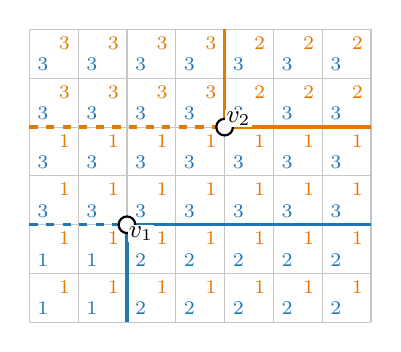
\begin{tikzpicture}[scale=0.62]
\draw[gedge] (0,0) grid (7,6);
\node[l1] at (0+0.28,0+0.28) {1};
\node[l2] at (0+0.72,0+0.72) {1};
\node[l1] at (0+0.28,1+0.28) {1};
\node[l2] at (0+0.72,1+0.72) {1};
\node[l1] at (0+0.28,2+0.28) {3};
\node[l2] at (0+0.72,2+0.72) {1};
\node[l1] at (0+0.28,3+0.28) {3};
\node[l2] at (0+0.72,3+0.72) {1};
\node[l1] at (0+0.28,4+0.28) {3};
\node[l2] at (0+0.72,4+0.72) {3};
\node[l1] at (0+0.28,5+0.28) {3};
\node[l2] at (0+0.72,5+0.72) {3};
\node[l1] at (1+0.28,0+0.28) {1};
\node[l2] at (1+0.72,0+0.72) {1};
\node[l1] at (1+0.28,1+0.28) {1};
\node[l2] at (1+0.72,1+0.72) {1};
\node[l1] at (1+0.28,2+0.28) {3};
\node[l2] at (1+0.72,2+0.72) {1};
\node[l1] at (1+0.28,3+0.28) {3};
\node[l2] at (1+0.72,3+0.72) {1};
\node[l1] at (1+0.28,4+0.28) {3};
\node[l2] at (1+0.72,4+0.72) {3};
\node[l1] at (1+0.28,5+0.28) {3};
\node[l2] at (1+0.72,5+0.72) {3};
\node[l1] at (2+0.28,0+0.28) {2};
\node[l2] at (2+0.72,0+0.72) {1};
\node[l1] at (2+0.28,1+0.28) {2};
\node[l2] at (2+0.72,1+0.72) {1};
\node[l1] at (2+0.28,2+0.28) {3};
\node[l2] at (2+0.72,2+0.72) {1};
\node[l1] at (2+0.28,3+0.28) {3};
\node[l2] at (2+0.72,3+0.72) {1};
\node[l1] at (2+0.28,4+0.28) {3};
\node[l2] at (2+0.72,4+0.72) {3};
\node[l1] at (2+0.28,5+0.28) {3};
\node[l2] at (2+0.72,5+0.72) {3};
\node[l1] at (3+0.28,0+0.28) {2};
\node[l2] at (3+0.72,0+0.72) {1};
\node[l1] at (3+0.28,1+0.28) {2};
\node[l2] at (3+0.72,1+0.72) {1};
\node[l1] at (3+0.28,2+0.28) {3};
\node[l2] at (3+0.72,2+0.72) {1};
\node[l1] at (3+0.28,3+0.28) {3};
\node[l2] at (3+0.72,3+0.72) {1};
\node[l1] at (3+0.28,4+0.28) {3};
\node[l2] at (3+0.72,4+0.72) {3};
\node[l1] at (3+0.28,5+0.28) {3};
\node[l2] at (3+0.72,5+0.72) {3};
\node[l1] at (4+0.28,0+0.28) {2};
\node[l2] at (4+0.72,0+0.72) {1};
\node[l1] at (4+0.28,1+0.28) {2};
\node[l2] at (4+0.72,1+0.72) {1};
\node[l1] at (4+0.28,2+0.28) {3};
\node[l2] at (4+0.72,2+0.72) {1};
\node[l1] at (4+0.28,3+0.28) {3};
\node[l2] at (4+0.72,3+0.72) {1};
\node[l1] at (4+0.28,4+0.28) {3};
\node[l2] at (4+0.72,4+0.72) {2};
\node[l1] at (4+0.28,5+0.28) {3};
\node[l2] at (4+0.72,5+0.72) {2};
\node[l1] at (5+0.28,0+0.28) {2};
\node[l2] at (5+0.72,0+0.72) {1};
\node[l1] at (5+0.28,1+0.28) {2};
\node[l2] at (5+0.72,1+0.72) {1};
\node[l1] at (5+0.28,2+0.28) {3};
\node[l2] at (5+0.72,2+0.72) {1};
\node[l1] at (5+0.28,3+0.28) {3};
\node[l2] at (5+0.72,3+0.72) {1};
\node[l1] at (5+0.28,4+0.28) {3};
\node[l2] at (5+0.72,4+0.72) {2};
\node[l1] at (5+0.28,5+0.28) {3};
\node[l2] at (5+0.72,5+0.72) {2};
\node[l1] at (6+0.28,0+0.28) {2};
\node[l2] at (6+0.72,0+0.72) {1};
\node[l1] at (6+0.28,1+0.28) {2};
\node[l2] at (6+0.72,1+0.72) {1};
\node[l1] at (6+0.28,2+0.28) {3};
\node[l2] at (6+0.72,2+0.72) {1};
\node[l1] at (6+0.28,3+0.28) {3};
\node[l2] at (6+0.72,3+0.72) {1};
\node[l1] at (6+0.28,4+0.28) {3};
\node[l2] at (6+0.72,4+0.72) {2};
\node[l1] at (6+0.28,5+0.28) {3};
\node[l2] at (6+0.72,5+0.72) {2};
\draw[bnd1] (2,2) -- (7,2);
\draw[bnd1] (2,0) -- (2,2);
\draw[slit1] (0,2) -- (2,2);
\draw[bnd2] (4,4) -- (7,4);
\draw[bnd2] (4,4) -- (4,6);
\draw[slit2] (0,4) -- (4,4);
\node[vort] at (2,2) {};
\node[vort] at (4,4) {};
\node[lab,fill=white,inner sep=0.5pt,below right] at (2,2) {$v_1$};
\node[lab,fill=white,inner sep=0.5pt,above right] at (4,4) {$v_2$};
\end{tikzpicture}\qquad
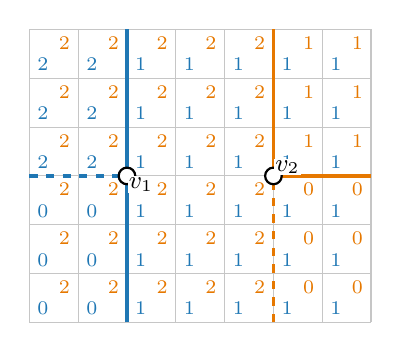
\begin{tikzpicture}[scale=0.62]
\draw[gedge] (0,0) grid (7,6);
\node[l1] at (0+0.28,0+0.28) {0};
\node[l2] at (0+0.72,0+0.72) {2};
\node[l1] at (0+0.28,1+0.28) {0};
\node[l2] at (0+0.72,1+0.72) {2};
\node[l1] at (0+0.28,2+0.28) {0};
\node[l2] at (0+0.72,2+0.72) {2};
\node[l1] at (0+0.28,3+0.28) {2};
\node[l2] at (0+0.72,3+0.72) {2};
\node[l1] at (0+0.28,4+0.28) {2};
\node[l2] at (0+0.72,4+0.72) {2};
\node[l1] at (0+0.28,5+0.28) {2};
\node[l2] at (0+0.72,5+0.72) {2};
\node[l1] at (1+0.28,0+0.28) {0};
\node[l2] at (1+0.72,0+0.72) {2};
\node[l1] at (1+0.28,1+0.28) {0};
\node[l2] at (1+0.72,1+0.72) {2};
\node[l1] at (1+0.28,2+0.28) {0};
\node[l2] at (1+0.72,2+0.72) {2};
\node[l1] at (1+0.28,3+0.28) {2};
\node[l2] at (1+0.72,3+0.72) {2};
\node[l1] at (1+0.28,4+0.28) {2};
\node[l2] at (1+0.72,4+0.72) {2};
\node[l1] at (1+0.28,5+0.28) {2};
\node[l2] at (1+0.72,5+0.72) {2};
\node[l1] at (2+0.28,0+0.28) {1};
\node[l2] at (2+0.72,0+0.72) {2};
\node[l1] at (2+0.28,1+0.28) {1};
\node[l2] at (2+0.72,1+0.72) {2};
\node[l1] at (2+0.28,2+0.28) {1};
\node[l2] at (2+0.72,2+0.72) {2};
\node[l1] at (2+0.28,3+0.28) {1};
\node[l2] at (2+0.72,3+0.72) {2};
\node[l1] at (2+0.28,4+0.28) {1};
\node[l2] at (2+0.72,4+0.72) {2};
\node[l1] at (2+0.28,5+0.28) {1};
\node[l2] at (2+0.72,5+0.72) {2};
\node[l1] at (3+0.28,0+0.28) {1};
\node[l2] at (3+0.72,0+0.72) {2};
\node[l1] at (3+0.28,1+0.28) {1};
\node[l2] at (3+0.72,1+0.72) {2};
\node[l1] at (3+0.28,2+0.28) {1};
\node[l2] at (3+0.72,2+0.72) {2};
\node[l1] at (3+0.28,3+0.28) {1};
\node[l2] at (3+0.72,3+0.72) {2};
\node[l1] at (3+0.28,4+0.28) {1};
\node[l2] at (3+0.72,4+0.72) {2};
\node[l1] at (3+0.28,5+0.28) {1};
\node[l2] at (3+0.72,5+0.72) {2};
\node[l1] at (4+0.28,0+0.28) {1};
\node[l2] at (4+0.72,0+0.72) {2};
\node[l1] at (4+0.28,1+0.28) {1};
\node[l2] at (4+0.72,1+0.72) {2};
\node[l1] at (4+0.28,2+0.28) {1};
\node[l2] at (4+0.72,2+0.72) {2};
\node[l1] at (4+0.28,3+0.28) {1};
\node[l2] at (4+0.72,3+0.72) {2};
\node[l1] at (4+0.28,4+0.28) {1};
\node[l2] at (4+0.72,4+0.72) {2};
\node[l1] at (4+0.28,5+0.28) {1};
\node[l2] at (4+0.72,5+0.72) {2};
\node[l1] at (5+0.28,0+0.28) {1};
\node[l2] at (5+0.72,0+0.72) {0};
\node[l1] at (5+0.28,1+0.28) {1};
\node[l2] at (5+0.72,1+0.72) {0};
\node[l1] at (5+0.28,2+0.28) {1};
\node[l2] at (5+0.72,2+0.72) {0};
\node[l1] at (5+0.28,3+0.28) {1};
\node[l2] at (5+0.72,3+0.72) {1};
\node[l1] at (5+0.28,4+0.28) {1};
\node[l2] at (5+0.72,4+0.72) {1};
\node[l1] at (5+0.28,5+0.28) {1};
\node[l2] at (5+0.72,5+0.72) {1};
\node[l1] at (6+0.28,0+0.28) {1};
\node[l2] at (6+0.72,0+0.72) {0};
\node[l1] at (6+0.28,1+0.28) {1};
\node[l2] at (6+0.72,1+0.72) {0};
\node[l1] at (6+0.28,2+0.28) {1};
\node[l2] at (6+0.72,2+0.72) {0};
\node[l1] at (6+0.28,3+0.28) {1};
\node[l2] at (6+0.72,3+0.72) {1};
\node[l1] at (6+0.28,4+0.28) {1};
\node[l2] at (6+0.72,4+0.72) {1};
\node[l1] at (6+0.28,5+0.28) {1};
\node[l2] at (6+0.72,5+0.72) {1};
\draw[bnd1] (2,0) -- (2,6);
\draw[slit1] (0,3) -- (2,3);
\draw[bnd2] (5,3) -- (5,6);
\draw[slit2] (5,0) -- (5,3);
\draw[bnd2] (5,3) -- (7,3);
\node[vort] at (2,3) {};
\node[vort] at (5,3) {};
\node[lab,fill=white,inner sep=0.5pt,below right] at (2,3) {$v_1$};
\node[lab,fill=white,inner sep=0.5pt,above right] at (5,3) {$v_2$};
\end{tikzpicture}

\caption{The three-sector labels of two vortices (open circles), computed from \lean{labD},
\lean{labU} (left) and \lean{labL}, \lean{labR} (right).
Each cell shows $\ell_1$ (blue, lower left) and $\ell_2$ (orange, upper right).
Solid lines are label boundaries with jump $\pm1$, and dashed lines are the slits, with jump
$\pm2$.
Left: different rows.
Right: one row.
No side lies on lines of both colours.}
\label{fig:twovortex}
\end{figure}

\begin{theorem}[\lean{arc\_vortex2}]
\label{thm:vortex2}
Under the hypotheses of \cref{thm:height2}, $H$ has no closed walk of arc steps between cells of
$V$ in a fixed direction.
\end{theorem}

\begin{proof}
Fix the direction $o$, put $g=\pm1$ as in \cref{thm:vortex}, and take $\tau,\delta_1,\delta_2$ from
\cref{thm:height2} with the slits above, so that a step from $c$ to $c'$ has
$\tau(c')-\tau(c)=\varepsilon+\delta_1k_1+\delta_2k_2$.
Put $\nu_i=-1$ if $g\delta_i=2$ and $\nu_i=1$ if $g\delta_i=-2$, so $g\delta_i=-2\nu_i$.
Define
\[\Phi(c)=3g\,\tau(c)+2\nu_1\ell_1(c)+2\nu_2\ell_2(c).\]
For a step whose arc points in direction $o$, $g\Delta\tau=1-2\nu_1k_1-2\nu_2k_2$, so
\[\Delta\Phi=3\,(1-2\nu_1k_1-2\nu_2k_2)+2\nu_1\Delta\ell_1+2\nu_2\Delta\ell_2.\]
Two geometric facts hold for every unit step (\lean{geo\_rows}, \lean{geo\_same}).
\begin{enumerate}[label=(G\arabic*)]
\item If $k_i=0$ then $|\Delta\ell_i|\le1$.
  If $k_i\ne0$ then $\Delta\ell_i=2k_i$.
\item At most one of the pairs $(k_1,\Delta\ell_1)$ and $(k_2,\Delta\ell_2)$ is nonzero.
\end{enumerate}
(G1) holds because the slit is exactly the boundary with jump $2$, and the jump is $+2$ in the
direction counted by $k_i=1$.
(G2) holds because the boundary rays of the two labels share no side.
For different rows, the two rows $y=b_1$ and $y=b_2$ are different lines, the downward ray of
$v_1$ lies below $b_1$, and the upward ray of $v_2$ lies above $b_2>b_1$.
For one row, the columns $x=a_1$ and $x=a_2$ differ, the left ray lies left of $a_1$, and the right
ray lies right of $a_2>a_1$.
Now there are three cases.
\begin{itemize}
\item Both pairs are zero.
  Then $\Delta\Phi=3$.
\item Pair $i$ is nonzero with $k_i=0$.
  Then $\Delta\Phi=3+2\nu_i\Delta\ell_i\ge3-2=1$.
\item Pair $i$ is nonzero with $k_i=\pm1$.
  Then $\Delta\ell_i=2k_i$ and $\Delta\Phi=3-6\nu_ik_i+4\nu_ik_i=3-2\nu_ik_i\ge1$.
\end{itemize}
So $\Phi$ rises by at least $1$ along every step, and no closed walk exists
(\lean{arc\_of\_pot}).
The case of $v_2$ below $v_1$, or left of it, follows by exchanging the names
(\lean{arc\_vortex2}).
\end{proof}

\begin{theorem}[\lean{twoHoleCase\_main}, \lean{HoleTwoVCost.lean}]
\label{thm:two}
For solid $V$ and distinct inner $s,t$, \lean{twoHoleCase} decides the problem within
$5\,217\,000\,(|V|+3)^6$ steps.
\end{theorem}

\begin{proof}
As for \cref{thm:one}, with two changes.
The deleted path now starts at the inner point $r=s$, so $G\cup P$ has the two vortices $t$ and $r$,
and \cref{thm:vortex2} replaces \cref{thm:vortex}.
Classes are pairs, all of them lie in $\lean{classRange}^2$, and \lean{classSearch} with two
prescribed values replaces \lean{classSearchOne} (\lean{kFind2\_solidFor}), with the same proof as
\cref{thm:classsearch}.
For the cost, there are again at most $208$ final tests, each at most $25\,000\,(|U|+3)^6$.
\end{proof}

% =====================================================================
\section{The algorithm and its running time}
\label{sec:time}

\lean{decideHamPath} tests whether each endpoint is inner (\lean{isInner}) and dispatches as in
\cref{tab:cases}.

\begin{table}[h]
\centering
\small
\begin{tabular}{@{}lllll@{}}
\toprule
$s$ & $t$ & algorithm & Lean theorem & bound \\
\midrule
not inner & not inner & \lean{boundaryEndpoints} & \lean{boundaryEndpoints\_main} & $1\,060\,000\,(|V|+3)^4$\\
not inner & inner & \lean{oneHoleCase} & \lean{oneHoleCase\_main} & $2\,513\,000\,(|V|+3)^5$\\
inner & not inner & \lean{oneHoleCase}, $s,t$ swapped & \lean{oneHoleCase\_main} & $2\,513\,000\,(|V|+3)^5$\\
inner & inner & \lean{twoHoleCase} & \lean{twoHoleCase\_main} & $5\,217\,000\,(|V|+3)^6$\\
\midrule
\multicolumn{3}{@{}l}{all cases, plus $10$ for the dispatch} & \lean{decideHamPath\_main} & $5\,220\,000\,(|V|+3)^6$\\
\bottomrule
\end{tabular}
\caption{The four cases of \lean{decideHamPath} and their proved bounds.
Swapping the endpoints in the third row uses that a path read backwards is a path
(\lean{hp\_swap}).}
\label{tab:cases}
\end{table}

\begin{proof}[Proof of \cref{thm:main}]
A point of $V$ that is not inner has a missing king neighbour (\lean{miss\_of\_not\_inner}).
So in each row of \cref{tab:cases} the hypotheses of the theorem named there hold, and
\cref{thm:bdry}, \cref{thm:one} or \cref{thm:two} applies, where the third row uses that a Hamiltonian $t$--$s$
path read backwards is a Hamiltonian $s$--$t$ path (\lean{hp\_swap}).
Each case decides the problem, and the largest bound plus $10$ for the dispatch is at most
$5\,220\,000\,(|V|+3)^6$.
\end{proof}

\paragraph{Where the exponents come from.}
One round of the fast loop (a phase and its reduction) costs at most $3000(|V|+3)^3$
(\lean{twoPhantomLoopCost\_le}).
The loop runs at most $|V|+2$ rounds, which gives degree $4$ (\lean{twoPhantomTestCost\_le}).
In the hole cases the loop runs once per class, and the class search costs $O(N^4)$ per class.
One hole has $2|U|+1$ classes, where $U$ is the set left after the deletions, which gives degree
$5$.
Two holes have $(2|U|+1)^2$ class pairs, which gives degree $6$.
The leading constants count the final tests of the deletion walks.
In the hole cases the two deletions before the walk give $4\cdot4=16$ walk starts, and each walk
makes at most $13$ final tests and visits at most $21$ nodes (\cref{par:ring}), so $208$ final tests
of cost at most $12\,000\,(|U|+3)^5$ (one hole) or $25\,000\,(|U|+3)^6$ (two holes).
When neither endpoint is inner, the initial $t$ may have no usable phantom and no deleted neighbour,
so the walk can branch into $4$ ring walks of at most $13$ final tests each, $52$ in all, and the
possible deletion of $s$ before it gives at most $4$ such walks.

\paragraph{Caveats.}
The cost functions charge unit cost for operations on finite sets of points and edges.
A machine implementation pays more for these operations, so its exponent can be larger, but it
stays polynomial.
The Lean statement does not link \lean{decideHamPathCost} to \lean{decideHamPath} formally.
The link is the parallel structure of the two definitions, which the reader checks.
The companion Umans--Lenhart formalization in the same repository uses a step-counting monad instead.

\paragraph{The walk constant: the ring potential.}
\label{par:ring}
Fix the walk's centre $w$ and its hole $t$ (when neither endpoint is inner, the centre $s$ and its
phantom $q$).
The king neighbours of $w$ other than $t$ form a path of $7$ points around $w$, the \emph{ring},
numbered $0,\dots,6$ (\lean{pidx}, \lean{ptAt}).
From ring point $i$ a lattice step goes to $w$, to $t$, to ring point $i\pm1$, or outward to king
distance $2$.
A corner of the ring has $2$ outward steps and an edge midpoint $1$ (\lean{outI},
\lean{cat\_counts}).
The walk continues only from a ring point, or from distance $2$ with an opposed phantom.
An outward step from the ring stops, since the phantom (the ring point just left) is not opposed.
Let the weight of a present ring point be its number of outward steps.
The leaf potential $L$ of a walk state is $0$ when at most $2$ points remain, $1$ at a stop, $13$ in
an opposed state, and on ring point $i$ the weight of $i$ plus the weights of the unbroken runs of
present ring points on both sides of $i$ (\lean{Lp}).
The $7$ weights sum to $11$, so $L\le13$.
A step along the ring to $i+1$ deletes $i$ and leaves the child with the run after $i$ only.
An outward step is a stop worth $1$, paid by the weight of $i$.
So the children's potentials sum to at most $L$ (\lean{ring\_step}).
An opposed state at king distance $2$ has four lattice steps.
One goes onto its phantom, which is absent, and the other three lead to states of potential at most
$11$, $1$ and $1$.
So its children sum to at most $11+1+1=13$ (\lean{opp\_step}).
Hence a walk makes at most $13$ final tests.
The node potential $M$ is defined like $L$, with each present ring point weighted by $1$ plus its
number of outward steps, and the same argument bounds the nodes of a walk by $21$
(\lean{holeCaseWalkCost\_pot}, \lean{boundaryEndpointsWalkCost\_pot}).
All facts about the ring are proved by \lean{decide}, which evaluates them exhaustively over the $4$
rotations and the $28$ relative positions of a walk state that the facts mention.

% SPDX-License-Identifier: CC0-1.0
%
% Pseudocode of the procedures that decideHamPath runs, transcribed from the Lean definitions.
% Requires in the preamble of hpst.tex:
%   \usepackage{algorithm}
%   \usepackage[noend]{algpseudocode}
% Uses \lean{...} from hpst.tex.
%
% Procedures are typeset in small capitals (\proc), helper predicates and functions in sans
% serif (\pfn), multi-letter variables in italics (\var).
%
\algrenewcommand{\textproc}{\textsc}
\algrenewcommand{\algorithmiccomment}[1]{\hfill{\small$\triangleright$~#1}}
\newcommand{\proc}[1]{\mbox{\textsc{#1}}}
\newcommand{\pfn}[1]{\textsf{#1}}
\newcommand{\var}[1]{\mathit{#1}}
\newcommand{\pctrue}{\textsf{true}}
\newcommand{\pcfalse}{\textsf{false}}
\newcommand{\pcnone}{\textsf{none}}
\newcommand{\pcbreak}{\textbf{break}}

\paragraph{Pseudocode.}
\proc{DecideHamPath} (\cref{alg:decideHamPath}) chooses one of three procedures by testing which
endpoints are inner.
Each walk deletes endpoints until the two out-vertices are Far with phantoms that are not opposed,
and then runs a final test.
The final test builds a path factor with \proc{FindFactor}, in the hole cases moves it into each
class with \proc{ClassSearch}, and runs the two-phantom loop \proc{TwoPhantomLoop}.
Each round of that loop is a \proc{RunPhase} followed by \proc{ReducePieces}.

The blocks below use the following conventions.
Each procedure has the name of its Lean definition, capitalised, and the caption of its block gives
that name.
All of these definitions are in \lean{Algorithm.lean}.
Helper predicates and functions are set in sans serif and are described after each block with
their Lean names.
$\pfn{Nbrs}(t)$ (Lean \lean{nbrsL}) is the list of pairs $(y,e)$ with $y$ a lattice neighbour of
$t$ and $e$ the edge $t$--$y$, in the order right, left, up, down.
The cells of $V$ are visited in lexicographic order (\lean{cellList}).
The procedures return Booleans, and \pctrue\ means that a Hamiltonian path exists.
Every loop over a list stops at its first success, as \lean{List.any}, \lean{List.find?} and
\lean{List.findSome?} do in Lean.
A loop ``for $n$ rounds'' runs at most $n$ times, and $n$ is the fuel of the Lean definition.

\begin{algorithm}[htbp]
\caption{\proc{DecideHamPath} (Lean \lean{decideHamPath})}
\label{alg:decideHamPath}
\begin{algorithmic}[1]
\Function{DecideHamPath}{$V,s,t$}
  \If{$\pfn{IsInner}(V,s)$}
    \If{$\pfn{IsInner}(V,t)$} \Return \Call{TwoHoleCase}{$V,s,t$}
      \Comment{both endpoints inner}
    \Else\ \Return \Call{OneHoleCase}{$V,t,s$}
      \Comment{only $s$ inner, read the path backwards}
    \EndIf
  \ElsIf{$\pfn{IsInner}(V,t)$} \Return \Call{OneHoleCase}{$V,s,t$}
    \Comment{only $t$ inner}
  \Else\ \Return \Call{BoundaryEndpoints}{$V,s,t$}
    \Comment{neither endpoint inner}
  \EndIf
\EndFunction
\end{algorithmic}
\end{algorithm}

In \cref{alg:decideHamPath}, $\pfn{IsInner}(V,p)$ (Lean \lean{isInner}) holds when the four squares with
corner $p$ are cells of $V$.

\begin{algorithm}[htbp]
\caption{\proc{BoundaryEndpoints} (Lean \lean{boundaryEndpoints})}
\label{alg:boundaryEndpoints}
\begin{algorithmic}[1]
\Function{BoundaryEndpoints}{$V,s,t$}
  \Comment{$s$ and $t$ each have a missing king neighbour}
  \If{$|V|\le2$} \Return [$s$ is a lattice neighbour of $t$]
  \EndIf
  \If{some $(q,e_{sq})\in\pfn{Nbrs}(s)$ has $q\notin V$ (take the first)}
    \Comment{$q$ becomes the phantom of $s$}
    \State \Return \Call{BoundaryEndpointsWalk}{$s,q,e_{sq},12,V,t$}
  \EndIf
  \ForAll{$(x,e)\in\pfn{Nbrs}(s)$ with $x\in V$, $x\ne t$}
    \Comment{delete $s$ (phantom of $x$)}
    \If{\Call{BoundaryEndpointsWalk}{$x,s,e,12,V\setminus\{s\},t$}} \Return \pctrue
    \EndIf
  \EndFor
  \State \Return \pcfalse
\EndFunction
\end{algorithmic}
\end{algorithm}

\begin{algorithm}[htbp]
\caption{\proc{BoundaryEndpointsWalk} (Lean \lean{boundaryEndpointsWalk})}
\label{alg:boundaryEndpointsWalk}
\begin{algorithmic}[1]
\Function{BoundaryEndpointsWalk}{$s,q,e_{sq},\var{fuel},V,t$}
  \Comment{$s$ keeps its phantom $q$, $t$ moves}
  \If{$\var{fuel}=0$} \Return \pcfalse
  \EndIf
  \If{$|V|\le2$} \Return [$s$ is a lattice neighbour of $t$]
  \EndIf
  \If{some $(p,e_{tp})\in\pfn{Nbrs}(t)$ has $\pfn{IsUsablePhantom}(V,s,q,t,p)$ (take the first)}
    \If{$\pfn{IsFar}(t,s)$}
      \Comment{$p$ is usable and $t$ is Far from $s$}
      \State \Return \Call{TwoPhantomTest}{$V,s,t,p,q,e_{tp},e_{sq}$}
      \Comment{the final test}
    \EndIf
  \EndIf
  \ForAll{$(x,\cdot)\in\pfn{Nbrs}(t)$ with $x\in V$, $x\ne s$}
    \Comment{delete $t$, $x$ is the next endpoint}
    \If{\Call{BoundaryEndpointsWalk}{$s,q,e_{sq},\var{fuel}-1,V\setminus\{t\},x$}} \Return \pctrue
    \EndIf
  \EndFor
  \State \Return \pcfalse
\EndFunction
\end{algorithmic}
\end{algorithm}

In \cref{alg:boundaryEndpoints,alg:boundaryEndpointsWalk}, $e_{sq}$ is the phantom edge $s$--$q$ and $e_{tp}$ is the phantom
edge $t$--$p$.
The fuel $12$ allows the at most $11$ deletion levels of \cref{sec:walk}.
$\pfn{IsUsablePhantom}(V,s,q,t,p)$ (Lean \lean{isUsablePhantom}) holds when $p\notin V$, $p\ne q$, and
the phantom $p$ of $t$ is not opposed to the phantom $q$ of $s$, so $p$ is a usable phantom.
$\pfn{IsFar}(t,s)$ (Lean \lean{isFar}) holds when $t=s$ or $\dist(t,s)\ge2$.

\begin{algorithm}[htbp]
\caption{\proc{HoleCase} (Lean \lean{holeCase}), \proc{OneHoleCase} (Lean
  \lean{oneHoleCase}) and \proc{TwoHoleCase} (Lean \lean{twoHoleCase})}
\label{alg:holeCase}
\label{alg:oneHoleCase}
\label{alg:twoHoleCase}
\begin{algorithmic}[1]
\Function{HoleCase}{$\var{finalTest},V,s,t$}
  \Comment{$t$ is inner}
  \If{$|V|\le2$} \Return [$s$ is a lattice neighbour of $t$]
  \EndIf
  \ForAll{$(w,e_{wt})\in\pfn{Nbrs}(t)$ with $w\in V$, $w\ne s$}
    \Comment{delete $t$ (phantom of $w$)}
    \If{$|V\setminus\{t\}|\le2$}
      \If{$s$ is a lattice neighbour of $w$} \Return \pctrue
      \EndIf
    \Else
      \ForAll{$(x,e)\in\pfn{Nbrs}(s)$ with $x\in V\setminus\{t\}$, $x\ne w$}
        \Comment{delete $s$ (phantom of $x$)}
        \If{\Call{HoleCaseWalk}{$\var{finalTest}(w,e_{wt}),w,t,10,V\setminus\{t,s\},x,s,e$}}
          \Return \pctrue
        \EndIf
      \EndFor
    \EndIf
  \EndFor
  \State \Return \pcfalse
\EndFunction
\Statex
\Function{OneHoleCase}{$V,s,t$}
  \Comment{$t$ inner, $s$ not inner}
  \State $\var{finalTest}(w,e_{wt})(U,s',q,e_{sq})\gets\Call{OneHoleFinalTest}{U,s',w,t,q,e_{wt},e_{sq}}$
  \State \Return \Call{HoleCase}{$\var{finalTest},V,s,t$}
\EndFunction
\Statex
\Function{TwoHoleCase}{$V,s,t$}
  \Comment{the original $s$ is the second hole}
  \State $\var{finalTest}(w,e_{wt})(U,s',q,e_{sq})\gets\Call{TwoHoleFinalTest}{U,s',w,t,s,q,e_{wt},e_{sq}}$
  \State \Return \Call{HoleCase}{$\var{finalTest},V,s,t$}
\EndFunction
\end{algorithmic}
\end{algorithm}

In \cref{alg:holeCase} the point $w$ is the neighbour of $t$ on the path, $e_{wt}$ is the edge
$w$--$t$, and the deleted $t$ is the phantom of $w$.
The argument $\var{finalTest}$ is a function of $(w,e_{wt})$ that returns the final test of the
walk.
In \proc{TwoHoleCase} the original $s$ is passed to \proc{TwoHoleFinalTest} as the second hole
$r$.

\begin{algorithm}[htbp]
\caption{\proc{HoleCaseWalk} (Lean \lean{holeCaseWalk})}
\label{alg:holeCaseWalk}
\begin{algorithmic}[1]
\Function{HoleCaseWalk}{$\var{finalTest},w,p_w,\var{fuel},U,s,q,e_{sq}$}
  \Comment{$w$ keeps its phantom $p_w$, $s$ moves}
  \If{$\var{fuel}=0$} \Return \pcfalse
  \EndIf
  \If{$|U|\le2$} \Return [$s$ is a lattice neighbour of $w$]
  \EndIf
  \If{$\pfn{IsFar}(w,s)$ and not $\pfn{PhantomsOpposed}(w,p_w,s,q)$}
    \Comment{ready for the final test}
    \State \Return $\var{finalTest}(U,s,q,e_{sq})$
  \EndIf
  \ForAll{$(x,e)\in\pfn{Nbrs}(s)$ with $x\in U$, $x\ne w$}
    \Comment{delete $s$ (phantom of $x$)}
    \If{\Call{HoleCaseWalk}{$\var{finalTest},w,p_w,\var{fuel}-1,U\setminus\{s\},x,s,e$}}
      \Return \pctrue
    \EndIf
  \EndFor
  \State \Return \pcfalse
\EndFunction
\end{algorithmic}
\end{algorithm}

In \cref{alg:holeCaseWalk} the phantom $p_w$ of $w$ is the deleted inner point $t$.
The phantom $q$ of $s$ is the point deleted last, and $e_{sq}$ is the edge $s$--$q$.
The fuel $10$ allows the at most $9$ deletions of \cref{sec:one}.
$\pfn{PhantomsOpposed}(a,m_a,b,m_b)$ (Lean \lean{phantomsOpposed}) holds when the phantoms $m_a$ of $a$ and
$m_b$ of $b$ are opposed (\cref{def:opp}).

\begin{algorithm}[htbp]
\caption{\proc{OneHoleFinalTest} (Lean \lean{oneHoleFinalTest}) and
  \proc{TwoHoleFinalTest} (Lean \lean{twoHoleFinalTest})}
\label{alg:oneHoleFinalTest}
\label{alg:twoHoleFinalTest}
\begin{algorithmic}[1]
\Function{OneHoleFinalTest}{$U,s,w,t,q,e_{wt},e_{sq}$}
  \Comment{hole at $t$}
  \If{not $\pfn{IsNarrow}(U)$} \Return \pcfalse
    \Comment{a wide set has no Hamiltonian path}
  \EndIf
  \State $R\gets\Call{FindFactor}{U,d_{sw}}$
  \Comment{a path factor with ends $s$ and $w$}
  \If{$R=\pcnone$} \Return \pcfalse
  \EndIf
  \State $F\gets R\cup\{e_{wt},e_{sq}\}$
  \Comment{the reference factor, phantoms $t$ and $q$}
  \For{$h=-|U|,\dots,|U|$}
    \Comment{every possible class (\lean{classRange})}
    \State $G\gets\Call{ClassSearch}{U,F,[t],[h]}$
    \Comment{a factor of class $h$ (\lean{classSearchOne})}
    \If{$G\ne\pcnone$ and \Call{TwoPhantomLoop}{$U,t,q,|U|+2,G$}} \Return \pctrue
    \EndIf
  \EndFor
  \State \Return \pcfalse
\EndFunction
\Statex
\Function{TwoHoleFinalTest}{$U,s,w,t,r,q,e_{wt},e_{sq}$}
  \Comment{holes at $t$ and $r$}
  \If{not $\pfn{IsNarrow}(U)$} \Return \pcfalse
  \EndIf
  \State $R\gets\Call{FindFactor}{U,d_{sw}}$
  \If{$R=\pcnone$} \Return \pcfalse
  \EndIf
  \State $F\gets R\cup\{e_{wt},e_{sq}\}$
  \For{$h_1=-|U|,\dots,|U|$}
    \For{$h_2=-|U|,\dots,|U|$}
      \Comment{every possible pair of classes}
      \State $G\gets\Call{ClassSearch}{U,F,[t,r],[h_1,h_2]}$
      \If{$G\ne\pcnone$ and \Call{TwoPhantomLoop}{$U,t,q,|U|+2,G$}} \Return \pctrue
      \EndIf
    \EndFor
  \EndFor
  \State \Return \pcfalse
\EndFunction
\end{algorithmic}
\end{algorithm}

In \cref{alg:oneHoleFinalTest}, $\pfn{IsNarrow}(U)$ (Lean \lean{isNarrow}) holds when the width and the
height of the bounding box of $U$ are both less than $|U|$.
The degrees $d_{sw}$ are $1$ at $s$ and $w$ and $2$ elsewhere.
The factor $F$ is a two-phantom factor on $U\cup\{t,q\}$ with phantoms $t$ of $w$ and $q$ of $s$.

\begin{algorithm}[htbp]
\caption{\proc{ClassSearch} (Lean \lean{classSearch}, with \lean{classPotential} and
  \lean{relaxA})}
\label{alg:classSearch}
\begin{algorithmic}[1]
\Function{ClassSearch}{$V,F,[a_1,\dots,a_k],[h_1,\dots,h_k]$}
  \Comment{hole $a_i$ gets class $h_i$}
  \State $\var{box}\gets\pfn{BoxSquares}(V)$
  \Comment{squares of the bounding box, $x$-major}
  \ForAll{$c\in\var{box}$}
    \Comment{start below every solution (\lean{kInitA})}
    \State $\varphi(c)\gets h_i$ for the first $i$ whose hole cell $a_i$ is $c$, else $-\pfn{BoxWidth}(V)$
  \EndFor
  \State $\varphi(c)\gets0$ for every square $c\notin\var{box}$
  \For{$|\var{box}|+1$ rounds}
    \Comment{Bellman--Ford relaxation (\lean{relaxA})}
    \State $\varphi'(c)\gets\max(\varphi(c),\pfn{LowerBound}(V,F,\varphi,c))$ for all
      $c\in\var{box}$
    \If{$\varphi'=\varphi$ on $\var{box}$} \pcbreak
      \Comment{fixed point, the least potential}
    \EndIf
    \State $\varphi\gets\varphi'$
  \EndFor
  \If{$\pfn{IsAdmissible}(V,F,[a_i],[h_i],\varphi)$}
    \Return $F\oplus\pfn{JumpEdges}(V,\varphi)$
    \Comment{the factor of these classes}
  \Else\ \Return \pcnone
    \Comment{no factor has these classes}
  \EndIf
\EndFunction
\end{algorithmic}
\end{algorithm}

In \cref{alg:classSearch}, $\pfn{BoxSquares}(V)$ (Lean \lean{boxSquares}) lists the squares of the bounding
box of $V$, and $\pfn{BoxWidth}(V)$ (Lean \lean{boxWidth}) is the width of that box.
Let $\sigma(e)$ be the sign of the arc of $F$ across $e$ ($+1$ from the lower or left square to the
upper or right one) when $e$ is an edge of $V$, and $0$ otherwise.
$\pfn{LowerBound}(V,F,\varphi,c)$ (Lean \lean{lowerBound}) is the largest lower bound on $\varphi(c)$
given by the four neighbours of $c$ under the constraint that each jump lies between $0$ and
$\sigma(e)$.
It is the maximum of $\varphi(c_\downarrow)+\min(0,\sigma)$ and
$\varphi(c_\leftarrow)+\min(0,\sigma)$ across the bottom and left sides and of
$\varphi(c_\uparrow)-\max(0,\sigma)$ and $\varphi(c_\rightarrow)-\max(0,\sigma)$ across the top
and right sides.
$\pfn{IsAdmissible}$ (Lean \lean{isAdmissible}) holds when every side of every square of the box has jump
$0$, or is an edge $e$ of $V$ with jump $\sigma(e)$, and $\varphi(a_i)=h_i$ for all $i$.
$\pfn{JumpEdges}(V,\varphi)$ (Lean \lean{jumpEdges}) is the set of edges of $V$ on sides of squares of the
box across which $\varphi$ jumps.
The rounds bound $|\var{box}|+1$ is \lean{kFuel}.
The potentials are stored in an array indexed by box position (\lean{toFA}).
With one hole, \proc{ClassSearch} is the Lean \lean{classSearchOne}.

\begin{algorithm}[htbp]
\caption{\proc{TwoPhantomTest} (Lean \lean{twoPhantomTest}) and
  \proc{TwoPhantomLoop} (Lean \lean{twoPhantomLoop})}
\label{alg:twoPhantomTest}
\label{alg:twoPhantomLoop}
\begin{algorithmic}[1]
\Function{TwoPhantomTest}{$V,s,t,p,q,e_{tp},e_{sq}$}
  \Comment{phantoms $p$ of $t$ and $q$ of $s$}
  \State $R\gets\Call{FindFactor}{V,d_{st}}$
  \Comment{a path factor with ends $s$ and $t$}
  \If{$R=\pcnone$} \Return \pcfalse
  \EndIf
  \State \Return \Call{TwoPhantomLoop}{$V,p,q,|V|+2,R\cup\{e_{tp},e_{sq}\}$}
  \Comment{add the phantom edges}
\EndFunction
\Statex
\Function{TwoPhantomLoop}{$V,p,q,\var{fuel},G$}
  \State $W\gets V\cup\{p,q\}$
  \For{$\var{fuel}$ rounds}
    \Comment{each round joins two pieces}
    \If{$\ncomp(W,G)=1$} \Return \pctrue
      \Comment{one piece, a Hamiltonian path}
    \EndIf
    \State $(H,\var{bridges},\var{outcome})\gets\Call{RunPhase}{V,W,|W|+1,G,[\,]}$
    \If{$\var{outcome}\in\{\textsf{stuck},\textsf{fuel}\}$} \Return \pcfalse
    \EndIf
    \State $G\gets\Call{ReducePieces}{V,W,H,\var{bridges},\var{outcome}}$
    \Comment{one piece fewer, no bridges}
  \EndFor
  \State \Return $[\ncomp(W,G)=1]$
\EndFunction
\end{algorithmic}
\end{algorithm}

\begin{algorithm}[htbp]
\caption{\proc{RunPhase} (Lean \lean{runPhase})}
\label{alg:runPhase}
\begin{algorithmic}[1]
\Function{RunPhase}{$V,W,\var{fuel},H,\var{bridges}$}
  \Comment{$\var{bridges}$ is listed newest first}
  \For{$\var{fuel}$ steps}
    \State $\var{conn}\gets\pfn{ConnectedPairs}(W,H)$
    \Comment{all pairs of points in one piece}
    \State $c\gets$ the first merging cell of $V$ that is not a pair square
    \Comment{\lean{findMergingCell}}
    \If{$c\ne\pcnone$} \Return $(H,\var{bridges},\textsf{merge}\ c)$
      \Comment{flipping $c$ joins two pieces}
    \EndIf
    \State $b\gets\pfn{FindRow}(V,\var{conn},H,\var{bridges})$
    \Comment{a critical cell whose row is not stuck}
    \If{$b=\pcnone$} \Return $(H,\var{bridges},\textsf{stuck})$
    \EndIf
    \If{$r_b$ is odd} \Return $(H,\var{bridges},\textsf{odd}\ b)$
      \Comment{lowering the odd row joins two pieces}
    \EndIf
    \If{$\pfn{FlipSplits}(W,H,b)$}
      \Comment{bridge step, undone or lowered later}
      \State flip $E_b$ in $H$, \quad $\var{bridges}\gets b::\var{bridges}$
      \Comment{one piece more}
    \Else\ \Return $(H,\var{bridges},\textsf{twist}\ b)$
      \Comment{even row, flipping $E_b$ splits nothing}
    \EndIf
  \EndFor
  \State \Return $(H,\var{bridges},\textsf{fuel})$
\EndFunction
\end{algorithmic}
\end{algorithm}

In \cref{alg:runPhase}, a bridge $b=(q_b,a_b,r_b)$ is a row of length $r_b$ from the cell $q_b$ in
the frame with front $a_b$, and $E_b$ is its last cell $c_{r_b-1}$.
Its fixed pair is $(c_{r_b-2},c_{r_b-1})$, and these two cells are \emph{pair squares} (Lean
\lean{pairSqB}).
$\pfn{ConnectedPairs}(W,H)$ (Lean \lean{connectedPairs}) is the set of pairs of points of $W$ that lie in one
piece of $H$.
A merging cell is an alternating cut cell (\lean{Alt}, \lean{isCutCell}).
$\pfn{FindRow}$ (Lean \lean{findRow}) scans the cells $q$ of $V$ in order and for each the sides
$a$ in the order bottom, top, left, right.
It returns $(q,a,r)$ for the first $q$ that is critical in frame $a$ with dark back and light front
(\lean{isCritical}), is not a square of any bridge, and has a row of length $r$ that is not stuck
(\lean{scanRow}).
\lean{scanRow} steps $j=1,2,\dots$ up to $|V|+1$ times.
It ends with a row of length $j$ when the front arc of $c_{j-1}$ differs from that of $q$, and it
ends stuck when $c_j$ is not a cell of $V$ or is a cut cell.
$\pfn{FlipSplits}(W,H,b)$ (Lean \lean{flipSplits}) holds when, after the flip of $E_b$, the corners
$b_1$ and $f_1$ of $E_b$ lie in different pieces.

\begin{algorithm}[htbp]
\caption{\proc{ReducePieces} (Lean \lean{reducePieces}) and
  \proc{UndoBridges} (Lean \lean{applyAll} and \lean{undoPlan})}
\label{alg:reducePieces}
\begin{algorithmic}[1]
\Function{ReducePieces}{$V,W,H,[b_1,\dots,b_k],\var{outcome}$}
  \Comment{$b_1$ is the newest bridge}
  \State $H_0\gets H$
  \For{$i=1,\dots,k$}
    \Comment{the states before each bridge (\lean{bridgeStatesConn})}
    \State $H_i\gets H_{i-1}$ with $E_{b_i}$ flipped, \quad $\var{conn}_i\gets\pfn{ConnectedPairs}(W,H_i)$
  \EndFor
  \If{$\var{outcome}=\textsf{merge}\ c$}
    \State $X\gets$ the first cell of $V$ with
      $\pfn{IsGoodMergingCell}(W,H,[b_i],[\var{conn}_i],X)$, else $c$
    \Comment{Theorem~R}
    \State $(u,v)\gets\pfn{MergePair}(H,X)$, \quad flip $X$ in $H$
    \Comment{half bridge}
  \ElsIf{$\var{outcome}=\textsf{odd}\ b$ or $\var{outcome}=\textsf{twist}\ b$}
    \State $(u,v)\gets\pfn{RowStartPair}(b)$
    \State flip the cells $c_{r_b-1},\dots,c_1,c_0$ of the row of $b$ in $H$
    \Comment{half bridge, lower the row}
  \Else\ \Return $H$
  \EndIf
  \State \Return \Call{UndoBridges}{$H,[b_1,\dots,b_k],[\var{conn}_1,\dots,\var{conn}_k],(u,v)$}
\EndFunction
\Statex
\Function{UndoBridges}{$H,[b_1,\dots,b_k],[\var{conn}_1,\dots,\var{conn}_k],(u,v)$}
  \Comment{$(u,v)$ is the pending pair}
  \For{$i=1,\dots,k$}
    \Comment{the plan (\lean{undoPlan})}
    \If{$u$ and $v$ are connected in $\var{conn}_i$}
      \Comment{joined before $b_i$ was made}
      \State $\var{op}_i\gets$ lower $b_i$, \quad $(u,v)\gets\pfn{RowStartPair}(b_i)$
    \Else\ $\var{op}_i\gets$ undo $b_i$
    \EndIf
  \EndFor
  \For{$i=1,\dots,k$}
    \Comment{apply the plan (\lean{applyAll})}
    \If{$\var{op}_i$ lowers $b_i$} flip the cells $c_{r_{b_i}-2},\dots,c_0$ of $b_i$ in $H$
    \Else\ flip $E_{b_i}$ in $H$
      \Comment{back to the state before $b_i$}
    \EndIf
  \EndFor
  \State \Return $H$
\EndFunction
\end{algorithmic}
\end{algorithm}

In \cref{alg:reducePieces}, $\var{conn}_i$ is the connection set of the state before bridge $b_i$
was made.
The half bridge joins the pieces of $u$ and $v$, and \proc{UndoBridges} removes the bridges while
keeping that join.
$\pfn{MergePair}(H,X)$ (Lean \lean{mergePair}) is the pair $(b_1,f_1)$ of $X$ in the frame with front
top when the bottom of $X$ is dark and front right otherwise (\lean{altFrame}).
$\pfn{RowStartPair}(b)$ (Lean \lean{rowStartPair}) is the pair $(b_1,f_1)$ of $q_b$ in the frame
$a_b$.
$\pfn{IsGoodMergingCell}$ (Lean \lean{isGoodMergingCell}) tests that $X$ is alternating, cut, and not a pair
square, and that every bridge $b_i$ whose square beyond $E_{b_i}$ is $X$ is lowered by the plan
started from $\pfn{MergePair}(H,X)$, so $X$ is good in the sense of Theorem~R.
The plan and the operations are computed and applied in the order $b_1,\dots,b_k$, newest bridge
first.

\begin{algorithm}[htbp]
\caption{\proc{FindFactor} (Lean \lean{findFactor} with \lean{augLoop}, \lean{augStep} and
  \lean{layerAcc}) and \proc{AugmentingWalk} (Lean \lean{walk})}
\label{alg:findFactor}
\begin{algorithmic}[1]
\Function{FindFactor}{$V,d$}
  \Comment{a factor with degrees $d$, or none}
  \State $F\gets\emptyset$
  \For{$|V|+1$ rounds}
    \Comment{one augmentation per round (\lean{augLoop})}
    \State $\var{layer}_0\gets\{z\in V : z \text{ black},\ \deg_F z<d(z)\}$
    \Comment{deficient black points}
    \For{$k=1,\dots,|V|$}
      \Comment{\lean{layerAcc}}
      \State $\var{layer}_k\gets\var{layer}_{k-1}\cup\pfn{AltNbrs}(V,F,\var{layer}_{k-1})$
    \EndFor
    \State $y\gets$ the least white $y\in\var{layer}_{|V|}$ with $\deg_F y<d(y)$
    \Comment{a deficient white end}
    \If{no such $y$} \pcbreak
      \Comment{no augmenting walk is left}
    \EndIf
    \State $F\gets\Call{AugmentingWalk}{V,F,[\var{layer}_{|V|-1},\dots,\var{layer}_0],y}$
  \EndFor
  \If{$\deg_F z=d(z)$ for all $z\in V$} \Return $F$
  \Else\ \Return \pcnone
  \EndIf
\EndFunction
\Statex
\Function{AugmentingWalk}{$V,F,[L_{n-1},\dots,L_0],v$}
  \Comment{walk from $v$ back to a black start}
  \State $F'\gets F$
  \For{$k=n-1,\dots,0$}
    \If{$v\notin L_k$}
      \Comment{step back into layer $k$}
      \State $e\gets$ the first edge $e$ at $v$ with $\pfn{IsBackEdge}(V,F,L_k,v,e)$
      \If{$e=\pcnone$} \Return $F'$
      \EndIf
      \State $F'\gets F'\setminus\{e\}$ if $v$ is black, else $F'\cup\{e\}$
      \Comment{toggle $e$}
      \State $v\gets$ the other end of $e$
    \EndIf
  \EndFor
  \State \Return $F'$
\EndFunction
\end{algorithmic}
\end{algorithm}

In \cref{alg:findFactor}, a point $(x,y)$ is black when $x+y$ is even and white otherwise.
$\pfn{AltNbrs}(V,F,u)$ (Lean \lean{nbr}) is the set of points joined to $u$ by an edge of $V$ that
is not in $F$ when $u$ is black and in $F$ when $u$ is white.
So $\var{layer}_k$ is the set of points reached from a deficient black point by an alternating
walk of at most $k$ steps.
$\pfn{IsBackEdge}(V,F,L,v,e)$ (Lean \lean{Bwd}) holds when $e$ is an edge of $V$ at $v$ whose other
end is in $L$, with $e\in F$ when $v$ is black and $e\notin F$ when $v$ is white.
It reads the factor $F$ of the start of the round, not $F'$.
The edges at $v$ are tried in the order right, left, up, down.
Each round toggles the edges of one augmenting walk from $y$ back to $\var{layer}_0$, and the
rounds stop when no deficient white point is reachable.


% =====================================================================
\section{Formal verification}
\label{sec:lean}

\paragraph{Structure.}
The proof is in the Lean~4 library \lean{SolidGridHam}~\cite{lean4} with Mathlib~\cite{mathlib2020}.
The toolchain is pinned to \lean{leanprover/lean4:v4.35.0-rc2} (\lean{lean/lean-toolchain}), and
Mathlib to the revision in \lean{lean/lake-manifest.json}.
The library, the reference implementations and this paper are at
\url{https://github.com/zzyzek/SolidGridGraphHamPath}.
The $s$--$t$ path development is in \lean{lean/SolidGridHam/Path/}, $98$ files and about $27{,}500$
lines.
The algorithm and every definition in the statement are in \lean{lean/SolidGridHam/Algorithm.lean},
about $950$ lines.
It builds on the grid, height and strip libraries of the companion Umans--Lenhart formalization
(\lean{ulhc\_main}) in the same repository.
\Cref{app:map} maps the ideas of this paper to modules.

\paragraph{Axioms.}
The command \lean{\#print axioms} applied to
\lean{SolidGridHam.HP.decideHamPath\_main} lists \lean{propext}, \lean{Classical.choice} and
\lean{Quot.sound}.
The same holds for \lean{stuck\_minimal} and \lean{arc\_vortex2}.
No file of the library contains \lean{sorry}, and the build has no warnings.

\paragraph{Trusted definitions.}
Lean checks every step of the proof.
The reader must check that the statement means what it should.
The definitions in the statement are \lean{Pt} ($\Z\times\Z$), \lean{Edge}, \lean{IsEdge},
\lean{deg}, \lean{IsFactor}, \lean{dST}, \lean{ncomp} and \lean{Solid}.
They are in \lean{Algorithm.lean}, together with every definition of the algorithm, so one file holds
everything the statement depends on.
The definition of \lean{Solid} was also cross-checked by computation against ``all interior faces
have unit area''.
For the step bound the reader must also check that \lean{decideHamPathCost} and the cost functions it calls
follow the structure of \lean{decideHamPath}, and accept the primitive costs (for example \lean{flipCost}
$=8$ in \lean{CostStrips.lean}, \lean{connBCost} in \lean{CostConn.lean}).
The algorithm \lean{decideHamPath} itself is computable.

\paragraph{Implementation.}
The repository contains reference implementations in Python, C and JavaScript, each with a command
line front end.
The Python implementation has two modes.
Its reference mode ports each definition on the call path of \lean{decideHamPath} as one function with
the same name, the same control flow, the same fuel constants and the same iteration orders.
Its fast mode adds answer-preserving speedups, and the C and JavaScript implementations port the
fast mode.
All of them return the path on a ``yes'' answer.
The implementations are not verified.

\paragraph{How to check.}
With \lean{elan} installed, run \lean{lake exe cache get} and \lean{lake build} in \lean{lean/}.
Then run \lean{lake env lean} on a file containing
\lean{import SolidGridHam.Path.HPFinal} and \lean{\#print axioms SolidGridHam.HP.decideHamPath\_main}.

% =====================================================================
\section{Worked example}
\label{sec:example}


\subsection{One complete run}
\label{sec:run}

Let $V$ be the $4\times4$ block $\{0,1,2,3\}^2$ without its top-left point $(0,3)$, so $|V|=15$, and
let $s=(0,2)$ and $t=(2,2)$ (\cref{fig:example}a).
$V$ is solid.
The point $t$ is inner and $s$ is not, so \lean{decideHamPath} (\textsc{DecideHamPath}, \cref{alg:decideHamPath})
calls $\lean{oneHoleCase}\ V\ s\ t$ (\textsc{OneHoleCase}, \cref{alg:oneHoleCase}).
This subsection follows that call from start to finish, in the order the algorithm executes it.
The run visits two leaves.
The first ends with a proof that it holds no Hamiltonian path, and the second finds one.
The run then stops, because every branching stops at its first success.

\begin{figure}[t]
\centering
% SPDX-License-Identifier: CC0-1.0
% Generated by gen.py; do not edit by hand.
\begin{tabular}{c@{\qquad}c@{\qquad}c@{\qquad}c}
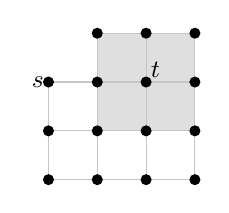
\begin{tikzpicture}[scale=0.62]
\fill[holecell] (1,1) rectangle (2,2);
\fill[holecell] (2,1) rectangle (3,2);
\fill[holecell] (1,2) rectangle (2,3);
\fill[holecell] (2,2) rectangle (3,3);
\draw[gedge] (0,0) -- (1,0);
\draw[gedge] (0,0) -- (0,1);
\draw[gedge] (0,1) -- (1,1);
\draw[gedge] (0,1) -- (0,2);
\draw[gedge] (0,2) -- (1,2);
\draw[gedge] (1,0) -- (2,0);
\draw[gedge] (1,0) -- (1,1);
\draw[gedge] (1,1) -- (2,1);
\draw[gedge] (1,1) -- (1,2);
\draw[gedge] (1,2) -- (2,2);
\draw[gedge] (1,2) -- (1,3);
\draw[gedge] (1,3) -- (2,3);
\draw[gedge] (2,0) -- (3,0);
\draw[gedge] (2,0) -- (2,1);
\draw[gedge] (2,1) -- (3,1);
\draw[gedge] (2,1) -- (2,2);
\draw[gedge] (2,2) -- (3,2);
\draw[gedge] (2,2) -- (2,3);
\draw[gedge] (2,3) -- (3,3);
\draw[gedge] (3,0) -- (3,1);
\draw[gedge] (3,1) -- (3,2);
\draw[gedge] (3,2) -- (3,3);
\node[pt] at (0,0) {};
\node[pt] at (0,1) {};
\node[pt] at (0,2) {};
\node[pt] at (1,0) {};
\node[pt] at (1,1) {};
\node[pt] at (1,2) {};
\node[pt] at (1,3) {};
\node[pt] at (2,0) {};
\node[pt] at (2,1) {};
\node[pt] at (2,2) {};
\node[pt] at (2,3) {};
\node[pt] at (3,0) {};
\node[pt] at (3,1) {};
\node[pt] at (3,2) {};
\node[pt] at (3,3) {};
\node[lab,left] at (0,2) {$s$};
\node[lab,above right] at (2,2) {$t$};
\end{tikzpicture} & \begin{tikzpicture}[scale=0.62]
\fill[holecell] (1,1) rectangle (2,2);
\fill[holecell] (2,1) rectangle (3,2);
\fill[holecell] (1,2) rectangle (2,3);
\fill[holecell] (2,2) rectangle (3,3);
\draw[gedge] (0,0) -- (1,0);
\draw[gedge] (0,0) -- (0,1);
\draw[gedge] (0,1) -- (1,1);
\draw[gedge] (1,0) -- (2,0);
\draw[gedge] (1,0) -- (1,1);
\draw[gedge] (1,1) -- (2,1);
\draw[gedge] (1,1) -- (1,2);
\draw[gedge] (1,2) -- (1,3);
\draw[gedge] (1,3) -- (2,3);
\draw[gedge] (2,0) -- (3,0);
\draw[gedge] (2,0) -- (2,1);
\draw[gedge] (2,1) -- (3,1);
\draw[gedge] (2,3) -- (3,3);
\draw[gedge] (3,0) -- (3,1);
\draw[gedge] (3,1) -- (3,2);
\draw[gedge] (3,2) -- (3,3);
\draw[ph] (2,2) -- (3,2);
\draw[ph] (0,2) -- (1,2);
\node[pt] at (0,0) {};
\node[pt] at (0,1) {};
\node[pt] at (1,0) {};
\node[pt] at (1,1) {};
\node[pt] at (1,2) {};
\node[pt] at (1,3) {};
\node[pt] at (2,0) {};
\node[pt] at (2,1) {};
\node[pt] at (2,3) {};
\node[pt] at (3,0) {};
\node[pt] at (3,1) {};
\node[pt] at (3,2) {};
\node[pt] at (3,3) {};
\node[miss] at (0,2) {};
\node[miss] at (2,2) {};
\node[lab,right] at (3,2) {$w$};
\node[lab,below right] at (1,2) {$x$};
\node[lab,left] at (0,2) {$q$};
\end{tikzpicture} & \begin{tikzpicture}[scale=0.62]
\fill[holecell] (1,1) rectangle (2,2);
\fill[holecell] (2,1) rectangle (3,2);
\fill[holecell] (1,2) rectangle (2,3);
\fill[holecell] (2,2) rectangle (3,3);
\fill[hicell] (1,0) rectangle (2,1);
\draw[gedge] (0,0) -- (1,0);
\draw[gedge] (0,0) -- (0,1);
\draw[gedge] (0,1) -- (1,1);
\draw[gedge] (1,0) -- (2,0);
\draw[gedge] (1,0) -- (1,1);
\draw[gedge] (1,1) -- (2,1);
\draw[gedge] (1,1) -- (1,2);
\draw[gedge] (1,2) -- (1,3);
\draw[gedge] (1,3) -- (2,3);
\draw[gedge] (2,0) -- (3,0);
\draw[gedge] (2,0) -- (2,1);
\draw[gedge] (2,1) -- (3,1);
\draw[gedge] (2,3) -- (3,3);
\draw[gedge] (3,0) -- (3,1);
\draw[gedge] (3,1) -- (3,2);
\draw[gedge] (3,2) -- (3,3);
\draw[pc1] (0,0) -- (1,0);
\draw[pc1] (0,1) -- (1,1);
\draw[pc1] (0,0) -- (0,1);
\draw[pc1] (1,0) -- (1,1);
\draw[pc2] (1,3) -- (2,3);
\draw[pc2] (2,3) -- (3,3);
\draw[pc2] (1,2) -- (1,3);
\draw[pc2] (3,2) -- (3,3);
\draw[pc3] (2,0) -- (3,0);
\draw[pc3] (2,1) -- (3,1);
\draw[pc3] (2,0) -- (2,1);
\draw[pc3] (3,0) -- (3,1);
\draw[ph] (2,2) -- (3,2);
\draw[ph] (0,2) -- (1,2);
\node[pt] at (0,0) {};
\node[pt] at (0,1) {};
\node[pt] at (1,0) {};
\node[pt] at (1,1) {};
\node[pt] at (1,2) {};
\node[pt] at (1,3) {};
\node[pt] at (2,0) {};
\node[pt] at (2,1) {};
\node[pt] at (2,3) {};
\node[pt] at (3,0) {};
\node[pt] at (3,1) {};
\node[pt] at (3,2) {};
\node[pt] at (3,3) {};
\node[miss] at (0,2) {};
\node[miss] at (2,2) {};
\node[lab,right] at (3,2) {$w$};
\node[lab,below right] at (1,2) {$x$};
\node[lab,left] at (0,2) {$q$};
\end{tikzpicture} & \begin{tikzpicture}[scale=0.62]
\fill[holecell] (1,1) rectangle (2,2);
\fill[holecell] (2,1) rectangle (3,2);
\fill[holecell] (1,2) rectangle (2,3);
\fill[holecell] (2,2) rectangle (3,3);
\draw[gedge] (0,0) -- (1,0);
\draw[gedge] (0,0) -- (0,1);
\draw[gedge] (0,1) -- (1,1);
\draw[gedge] (1,0) -- (2,0);
\draw[gedge] (1,0) -- (1,1);
\draw[gedge] (1,1) -- (2,1);
\draw[gedge] (1,1) -- (1,2);
\draw[gedge] (1,2) -- (1,3);
\draw[gedge] (1,3) -- (2,3);
\draw[gedge] (2,0) -- (3,0);
\draw[gedge] (2,0) -- (2,1);
\draw[gedge] (2,1) -- (3,1);
\draw[gedge] (2,3) -- (3,3);
\draw[gedge] (3,0) -- (3,1);
\draw[gedge] (3,1) -- (3,2);
\draw[gedge] (3,2) -- (3,3);
\draw[pc1] (0,0) -- (1,0);
\draw[pc1] (0,1) -- (1,1);
\draw[pc1] (1,0) -- (2,0);
\draw[pc1] (1,1) -- (2,1);
\draw[pc1] (2,0) -- (3,0);
\draw[pc1] (2,1) -- (3,1);
\draw[pc1] (0,0) -- (0,1);
\draw[pc1] (3,0) -- (3,1);
\draw[pc2] (1,3) -- (2,3);
\draw[pc2] (2,3) -- (3,3);
\draw[pc2] (1,2) -- (1,3);
\draw[pc2] (3,2) -- (3,3);
\draw[ph] (2,2) -- (3,2);
\draw[ph] (0,2) -- (1,2);
\node[pt] at (0,0) {};
\node[pt] at (0,1) {};
\node[pt] at (1,0) {};
\node[pt] at (1,1) {};
\node[pt] at (1,2) {};
\node[pt] at (1,3) {};
\node[pt] at (2,0) {};
\node[pt] at (2,1) {};
\node[pt] at (2,3) {};
\node[pt] at (3,0) {};
\node[pt] at (3,1) {};
\node[pt] at (3,2) {};
\node[pt] at (3,3) {};
\node[miss] at (0,2) {};
\node[miss] at (2,2) {};
\node[lab,right] at (3,2) {$w$};
\node[lab,below right] at (1,2) {$x$};
\node[lab,left] at (0,2) {$q$};
\end{tikzpicture} \\
\small (a) input & \small (b) leaf 1 & \small (c) 3 pieces & \small (d) stuck, $2$ pieces
\end{tabular}\\[8pt]
\begin{tabular}{c@{\qquad}c@{\qquad}c}
\begin{tikzpicture}[scale=0.62]
\fill[holecell] (1,1) rectangle (2,2);
\fill[holecell] (2,1) rectangle (3,2);
\fill[holecell] (1,2) rectangle (2,3);
\fill[holecell] (2,2) rectangle (3,3);
\fill[hicell] (1,0) rectangle (2,1);
\draw[gedge] (0,0) -- (1,0);
\draw[gedge] (0,0) -- (0,1);
\draw[gedge] (0,1) -- (1,1);
\draw[gedge] (1,0) -- (2,0);
\draw[gedge] (1,0) -- (1,1);
\draw[gedge] (1,1) -- (2,1);
\draw[gedge] (1,1) -- (1,2);
\draw[gedge] (1,2) -- (1,3);
\draw[gedge] (1,3) -- (2,3);
\draw[gedge] (2,0) -- (3,0);
\draw[gedge] (2,0) -- (2,1);
\draw[gedge] (2,1) -- (3,1);
\draw[gedge] (2,3) -- (3,3);
\draw[gedge] (3,0) -- (3,1);
\draw[gedge] (3,1) -- (3,2);
\draw[gedge] (3,2) -- (3,3);
\draw[pc1] (0,0) -- (1,0);
\draw[pc1] (1,3) -- (2,3);
\draw[pc1] (2,3) -- (3,3);
\draw[pc1] (0,0) -- (0,1);
\draw[pc1] (1,0) -- (1,1);
\draw[pc1] (1,1) -- (1,2);
\draw[pc1] (1,2) -- (1,3);
\draw[pc1] (3,2) -- (3,3);
\draw[pc2] (2,0) -- (3,0);
\draw[pc2] (2,1) -- (3,1);
\draw[pc2] (2,0) -- (2,1);
\draw[pc2] (3,0) -- (3,1);
\draw[ph] (2,2) -- (3,2);
\draw[ph] (0,1) -- (0,2);
\node[pt] at (0,0) {};
\node[pt] at (0,1) {};
\node[pt] at (1,0) {};
\node[pt] at (1,1) {};
\node[pt] at (1,2) {};
\node[pt] at (1,3) {};
\node[pt] at (2,0) {};
\node[pt] at (2,1) {};
\node[pt] at (2,3) {};
\node[pt] at (3,0) {};
\node[pt] at (3,1) {};
\node[pt] at (3,2) {};
\node[pt] at (3,3) {};
\node[miss] at (0,2) {};
\node[miss] at (2,2) {};
\node[lab,right] at (3,2) {$w$};
\node[lab,left] at (0,1) {$x$};
\node[lab,left] at (0,2) {$q$};
\end{tikzpicture} & \begin{tikzpicture}[scale=0.62]
\fill[holecell] (1,1) rectangle (2,2);
\fill[holecell] (2,1) rectangle (3,2);
\fill[holecell] (1,2) rectangle (2,3);
\fill[holecell] (2,2) rectangle (3,3);
\draw[gedge] (0,0) -- (1,0);
\draw[gedge] (0,0) -- (0,1);
\draw[gedge] (0,1) -- (1,1);
\draw[gedge] (1,0) -- (2,0);
\draw[gedge] (1,0) -- (1,1);
\draw[gedge] (1,1) -- (2,1);
\draw[gedge] (1,1) -- (1,2);
\draw[gedge] (1,2) -- (1,3);
\draw[gedge] (1,3) -- (2,3);
\draw[gedge] (2,0) -- (3,0);
\draw[gedge] (2,0) -- (2,1);
\draw[gedge] (2,1) -- (3,1);
\draw[gedge] (2,3) -- (3,3);
\draw[gedge] (3,0) -- (3,1);
\draw[gedge] (3,1) -- (3,2);
\draw[gedge] (3,2) -- (3,3);
\draw[pc1] (0,0) -- (1,0);
\draw[pc1] (1,0) -- (2,0);
\draw[pc1] (1,1) -- (2,1);
\draw[pc1] (1,3) -- (2,3);
\draw[pc1] (2,0) -- (3,0);
\draw[pc1] (2,1) -- (3,1);
\draw[pc1] (2,3) -- (3,3);
\draw[pc1] (0,0) -- (0,1);
\draw[pc1] (1,1) -- (1,2);
\draw[pc1] (1,2) -- (1,3);
\draw[pc1] (3,0) -- (3,1);
\draw[pc1] (3,2) -- (3,3);
\draw[ph] (2,2) -- (3,2);
\draw[ph] (0,1) -- (0,2);
\node[pt] at (0,0) {};
\node[pt] at (0,1) {};
\node[pt] at (1,0) {};
\node[pt] at (1,1) {};
\node[pt] at (1,2) {};
\node[pt] at (1,3) {};
\node[pt] at (2,0) {};
\node[pt] at (2,1) {};
\node[pt] at (2,3) {};
\node[pt] at (3,0) {};
\node[pt] at (3,1) {};
\node[pt] at (3,2) {};
\node[pt] at (3,3) {};
\node[miss] at (0,2) {};
\node[miss] at (2,2) {};
\node[lab,right] at (3,2) {$w$};
\node[lab,left] at (0,1) {$x$};
\node[lab,left] at (0,2) {$q$};
\end{tikzpicture} & \begin{tikzpicture}[scale=0.62]
\fill[holecell] (1,1) rectangle (2,2);
\fill[holecell] (2,1) rectangle (3,2);
\fill[holecell] (1,2) rectangle (2,3);
\fill[holecell] (2,2) rectangle (3,3);
\draw[gedge] (0,0) -- (1,0);
\draw[gedge] (0,0) -- (0,1);
\draw[gedge] (0,1) -- (1,1);
\draw[gedge] (0,1) -- (0,2);
\draw[gedge] (0,2) -- (1,2);
\draw[gedge] (1,0) -- (2,0);
\draw[gedge] (1,0) -- (1,1);
\draw[gedge] (1,1) -- (2,1);
\draw[gedge] (1,1) -- (1,2);
\draw[gedge] (1,2) -- (2,2);
\draw[gedge] (1,2) -- (1,3);
\draw[gedge] (1,3) -- (2,3);
\draw[gedge] (2,0) -- (3,0);
\draw[gedge] (2,0) -- (2,1);
\draw[gedge] (2,1) -- (3,1);
\draw[gedge] (2,1) -- (2,2);
\draw[gedge] (2,2) -- (3,2);
\draw[gedge] (2,2) -- (2,3);
\draw[gedge] (2,3) -- (3,3);
\draw[gedge] (3,0) -- (3,1);
\draw[gedge] (3,1) -- (3,2);
\draw[gedge] (3,2) -- (3,3);
\draw[pc1] (0,0) -- (1,0);
\draw[pc1] (1,0) -- (2,0);
\draw[pc1] (1,1) -- (2,1);
\draw[pc1] (1,3) -- (2,3);
\draw[pc1] (2,0) -- (3,0);
\draw[pc1] (2,1) -- (3,1);
\draw[pc1] (2,2) -- (3,2);
\draw[pc1] (2,3) -- (3,3);
\draw[pc1] (0,0) -- (0,1);
\draw[pc1] (0,1) -- (0,2);
\draw[pc1] (1,1) -- (1,2);
\draw[pc1] (1,2) -- (1,3);
\draw[pc1] (3,0) -- (3,1);
\draw[pc1] (3,2) -- (3,3);
\node[pt] at (0,0) {};
\node[pt] at (0,1) {};
\node[pt] at (0,2) {};
\node[pt] at (1,0) {};
\node[pt] at (1,1) {};
\node[pt] at (1,2) {};
\node[pt] at (1,3) {};
\node[pt] at (2,0) {};
\node[pt] at (2,1) {};
\node[pt] at (2,2) {};
\node[pt] at (2,3) {};
\node[pt] at (3,0) {};
\node[pt] at (3,1) {};
\node[pt] at (3,2) {};
\node[pt] at (3,3) {};
\node[lab,left] at (0,2) {$s$};
\node[lab,above right] at (2,2) {$t$};
\end{tikzpicture} \\
\small (e) 2 pieces & \small (f) $1$ piece & \small (g) the answer
\end{tabular}

\caption{One run of \lean{decideHamPath} on $15$ points, in execution order.
Red circles are deleted points, dashed teal edges are phantom edges, grey squares are the four
cells around the inner endpoint $t$, and yellow cells are merging cells.
Pieces are coloured blue, red and green.
(a) The input.
(b) Leaf~1.
$t$ is deleted and its first neighbour $w=(3,2)$ gets the phantom $t$.
$s$ is deleted and its first neighbour $x=(1,2)$ gets the phantom $q=s$.
$x$ and $w$ are Far, so the walk stops at once.
(c) The least factor of the only nonempty class, with $3$ pieces, and its merging cell $(1,0)$.
(d) After the flip, $2$ pieces, and the phase ends stuck.
The certificate shows that no factor of the class has one piece, so leaf~1 answers no.
(e) Leaf~2, the next successor $x=(0,1)$ of $s$.
The least factor of the class has $2$ pieces and the merging cell $(1,0)$.
(f) After the flip, $1$ piece.
(g) Adding back $s$ and $t$ gives a Hamiltonian $s$--$t$ path, and the run stops.}
\label{fig:example}
\end{figure}

\paragraph{Deletions.}
The algorithm deletes $t$ and tries its neighbours $w\ne s$ in the order right, left, up, down.
The first is $w=(3,2)$, which gets $t$ as its phantom.
It then deletes $s$ and tries the neighbours $x\ne w$ of $s$ in the same order.
The first is $x=(1,2)$, which gets $q=s$ as its phantom.
The king distance of $x$ and $w$ is $2$, so they are Far, and the phantoms are not opposed.
The walk therefore stops before deleting anything else, and the final test \lean{oneHoleFinalTest} (\textsc{OneHoleFinalTest}, \cref{alg:oneHoleFinalTest}) runs on
$U=V\setminus\{s,t\}$.
This leaf asks whether $V$ has a Hamiltonian path that starts with the edge $s$--$(1,2)$ and ends
with the edge $(3,2)$--$t$.

\paragraph{Leaf 1, the class search.}
\lean{findFactor} returns a factor with $2$ pieces.
The final test then tries the classes $h=-13,\dots,13$ in order.
For each $h$, \lean{classSearchOne} returns the least factor whose relative height at the hole cell of $t$ is
$h$, or nothing (\cref{sec:classes}).
Only $h=0$ gives a factor here.
It has $3$ pieces, a $4$-cycle on $(0,0),(1,0),(0,1),(1,1)$, a $4$-cycle on $(2,0),(3,0),(2,1),(3,1)$,
and the path piece through the top two rows (\cref{fig:example}c).

\paragraph{Leaf 1, the loop.}
The first phase finds the merging cell $(1,0)$ between the two $4$-cycles.
The reduction flips it, which joins the two cycles into an $8$-cycle.
The second phase finds no merging cell and no critical cell that is not stuck, so it ends stuck
with $2$ pieces and no bridges.
By the certificate (\cref{thm:cert}), every factor of this class has at least $2$ pieces.
Since $h=0$ is the only nonempty class, leaf~1 has no Hamiltonian path, and the algorithm moves on.

\paragraph{Leaf 2.}
The next neighbour of $s$ is $x=(0,1)$, whose king distance to $w$ is $3$.
Again the walk stops at once and only $h=0$ gives a factor.
This factor has $2$ pieces, the $4$-cycle on $(2,0),(3,0),(2,1),(3,1)$ and the path piece
(\cref{fig:example}e).
The first phase finds the merging cell $(1,0)$, and the flip leaves $1$ piece.
The loop answers yes, and adding back $s$ and $t$ gives the Hamiltonian path
\[(0,2),(0,1),(0,0),(1,0),(2,0),(3,0),(3,1),(2,1),(1,1),(1,2),(1,3),(2,3),(3,3),(3,2),(2,2).\]
The remaining branches are never evaluated.

\subsection{Inside the leaves of a $4\times4$ instance}
\label{sec:inside}

This subsection is not a run.
It takes the $4\times4$ block $V=\{0,1,2,3\}^2$ with $s=(3,0)$ and inner $t=(1,1)$, and looks inside
individual leaves to show a longer walk, the four factors of a class, and the slit height.
\Cref{fig:walk,fig:flip,fig:vortex} use this instance.

Consider the branch $w=(1,0)$ and $x=(2,0)$.
Here $\dist(x,w)=1$, so the walk deletes $(2,0)$.
Its only successor other than $w$ is $(2,1)$, again at king distance $1$ from $w$, so the walk
deletes $(2,1)$ too.
Both successors of $(2,1)$, namely $(3,1)$ and $(2,2)$, are at king distance $2$ from $w$, with
phantom $(2,1)$, not opposed to $t$.
The leaf for $(3,1)$ has $U=V\setminus\{t,(3,0),(2,0),(2,1)\}$, endpoint $(3,1)$, phantom
$q=(2,1)$, and deleted path $P=(3,0)$--$(2,0)$--$(2,1)$ (\cref{fig:walk}, right).
The set $U$ has exactly one Hamiltonian path from $(3,1)$ to $(1,0)$,
\[(3,1),(3,2),(3,3),(2,3),(2,2),(1,2),(1,3),(0,3),(0,2),(0,1),(0,0),(1,0).\]
Adding back $t$ and the deleted path gives a Hamiltonian path of $V$ from $s$ to $t$.

At this leaf the point $(2,1)$ is inner in $V$ and missing from $U$.
In $G\cup P$ it has one edge from $P$ and one phantom edge from $G$, so its degree is $2$
(\cref{lem:wsdeg}).
Had the phantom of $(3,1)$ been the missing point $(3,0)$, the point $(2,1)$ would have degree $1$ and
would be a second vortex.

\paragraph{Factors and class.}
Take the leaf $w=(0,1)$, $x=(3,1)$.
Here $\dist(x,w)=3$, so the walk stops at once with $U=V\setminus\{t,s\}$ and phantom $q=s$.
The setting is a two-phantom factor on $W=V$ with degree $1$ at the phantoms $t$ and $q$, containing
$w$--$t$ and $x$--$q$.
The cells of $U$ are $(0,2)$, $(1,2)$, $(2,1)$ and $(2,2)$.
There are exactly four such factors, $G_0,\dots,G_3$.
\begin{center}
\begin{tabular}{@{}cccl@{}}
\toprule
factor & pieces & $D(G_0,G_k)\ne0$ at & merging cells \\
\midrule
$G_0$ & 2 & none & $(1,2)$ \\
$G_1$ & 3 & $(2,1)$ & $(1,2)$, $(2,1)$ \\
$G_2$ & 1 & $(1,2)$ & none \\
$G_3$ & 2 & $(2,1)$, $(1,2)$ & $(2,1)$ \\
\bottomrule
\end{tabular}
\end{center}
Every nonzero value of $D(G_0,G_k)$ in the table equals $2$.
In particular $D(G_0,G_k)=0$ at the hole cell $t$ for all $k$, so all four factors lie in one class.
Here \lean{findFactor} returns $G_1$, so the reference factor is $F=G_1$.
The admissible potentials are $D(G_1,G_k)/2$.
They are $0$ for $G_1$, $-1$ at $(2,1)$ for $G_0$, $-1$ at $(2,1)$ and $1$ at $(1,2)$ for $G_2$, and
$1$ at $(1,2)$ for $G_3$, and $0$ elsewhere.
The least one with value $0$ at $t$ is that of $G_0$, so \lean{classSearchOne} returns $G_0$ for $h=0$ and
nothing for $h\ne0$.

\paragraph{The factor $G_0$.}
$G_0$ consists of the path piece
\[t,\ (0,1),\ (0,0),\ (1,0),\ (2,0),\ (2,1),\ (2,2),\ (2,3),\ (3,3),\ (3,2),\ (3,1),\ q\]
and the $4$-cycle around the cell $(0,2)$ (\cref{fig:flip}, left).
The cell $(1,2)$ has dark left and right sides and light top and bottom.
Its left corners lie on the cycle and its right corners on the path, so it is a merging cell.

\paragraph{Arcs, slit height and potential.}
The deleted path is the single point $s$, with no edges, so $G_0\cup P=G_0$ on $V$.
Its only inner point of degree $1$ is $t$.
The slit of $t=(1,1)$ is the side between the cells $(0,0)$ and $(0,1)$.
Solving the jump equations of \cref{thm:slit} on the nine cells is consistent only for $\delta=-2$.
The resulting heights, shifted so the least is $0$, are shown in \cref{fig:vortex} (right).
\begin{center}
\begin{tabular}{@{}c|ccc@{}}
$y\backslash x$ & 0 & 1 & 2\\\hline
2 & 1 & 2 & 1\\
1 & 0 & 1 & 2\\
0 & 3 & 2 & 1
\end{tabular}
\end{center}
Going once counterclockwise around $t$ through the cells $(0,0),(1,0),(1,1),(0,1)$, the arcs give
$-1,-1,-1,+1$, a total of $-2$.
This is the vortex.
For $o=\lean{true}$ we have $g=1$, $g\delta=-2$ and $\nu=1$, so $\Phi=2\tau+\lab$.
Its values are $6,5,3$ on the bottom row (left to right), $3,4,6$ on the middle row and $5,6,4$ on
the top row.
Each of the twelve arcs between these cells goes from a smaller to a larger value of $\Phi$.
For example, the arc across the slit points from $(0,1)$ to $(0,0)$, and $\Phi$ goes from $3$ to $6$.

Flipping the merging cell $(1,2)$ of $G_0$ gives $G_2$, with one piece (\cref{fig:flip}).

% =====================================================================
\section{The bulk case: endpoints far apart}
\label{sec:bulk}

Most of the paper is spent on moving the endpoints, because the proof must handle every position of
$s$ and $t$.
When $s$ and $t$ are far apart, the walks stop at once and the work is elsewhere.
This section describes what the algorithm does then, with one run on $34$ points
(\cref{fig:bulk}), whose endpoints are at king distance $3$ and whose walks also stop at once.

\paragraph{The endpoints cost little.}
Deleting $t$ (branch $w$) and $s$ (branch $x$) moves each endpoint by one step.
If $s$ and $t$ are at king distance at least $4$, then $w$ and $x$ are at king distance at least
$2$, so they are Far.
Their phantoms can be opposed only when $w$ and $x$ differ by exactly $2$ along an axis
(\cref{def:opp}), which needs king distance exactly $4$ between $s$ and $t$.
So when $s$ and $t$ are at king distance at least $5$, every walk stops at once and calls the final
test.
There are at most $4\cdot4=16$ such leaves, and they are tried one after another until one
succeeds.

\paragraph{Inner endpoints become holes.}
An inner endpoint has all eight king neighbours in $V$.
After its deletion it is a hole of $U$, surrounded by four cells (grey in \cref{fig:bulk}).
A factor of $U$ with its two phantom edges has degree $1$ at the hole, and its height field turns
around it like a vortex (\cref{sec:vortex}).
Factors are grouped into classes by the relative height $D$ at the cells around each hole.
Within one class, the phase and the certificate work as in Sheffield's cycle algorithm, because
the slit height and the quadrant label give a potential that rises along every climb
(\cref{sec:vortex}), and with two holes the three-sector labels do (\cref{sec:two}).
Across classes they need not, so the final test runs Sheffield's loop once per class.

\paragraph{What the final test does.}
For one hole there are at most $2|U|+1$ classes, and for two holes at most $(2|U|+1)^2$ pairs.
For each class, \lean{classSearch} returns the least factor of the class, or nothing when the class is
empty (\cref{sec:classes}).
In the runs of \cref{sec:run} and of this section exactly one class, or class pair, is nonempty.
The least factor of a class is the starting state of the loop.
It can have more pieces than the factor \lean{findFactor} found, because it is chosen for its heights
and not for its pieces.

\paragraph{The moves of the loop.}
Each round of the loop is one phase and one reduction, and it lowers the number of pieces by one
(\cref{sec:undo,sec:loop}).
A phase makes moves of three kinds.
\begin{itemize}
\item A \emph{merge} flips an alternating cell whose corners lie in two pieces.
  The two pieces become one.
\item A \emph{bridge step} is used when no such cell exists.
  It takes a critical cell, follows its row to the last cell where the heights turn, and flips that
  last cell.
  The flip splits a piece, so the count goes up by one, but it exposes new cells.
\item An \emph{odd row} or a \emph{twist} ends the phase like a merge.
\end{itemize}
The reduction then applies the half bridge (the flip of the merging cell, or the lowering of the
row), and walks back through the bridges,
newest first.
Each bridge is either lowered (the cells of its row before the last are flipped) or undone (its last
cell is flipped back), as the plan of \cref{sec:undo} decides.
The net effect of a round is one piece fewer.
If a phase ends stuck, no merge, bridge step or row is available, and the certificate shows that no
factor of the class has fewer pieces than the phase started with.
The loop then gives up on this class.

\paragraph{The example.}
\Cref{fig:bulk} shows a run on a $6\times6$ block with two points removed from the left column.
Both endpoints $s=(4,4)$ and $t=(4,1)$ are inner, at king distance $3$, so \lean{decideHamPath} calls
\lean{twoHoleCase} (\textsc{TwoHoleCase}).
The first branch, $w=(5,1)$ and $x=(5,4)$, already succeeds.
\begin{itemize}
\item Deleting $t$ and $s$ leaves $U$ with $32$ points and two holes.
  The walk takes no step, since $w$ and $x$ are at king distance $3$.
\item \lean{findFactor} returns a factor with $2$ pieces.
  The only nonempty class pair is $(0,0)$, and its least factor has $4$ pieces, a long path and
  three $4$-cycles (\cref{fig:bulk}c).
\item Phase~1 flips the merging cell $(1,4)$ and joins the top-left cycle to the path.
  Phase~2 flips $(2,0)$ and joins a second $4$-cycle to the path.
\item Phase~3 starts with $2$ pieces, the path and the cycle on $(4,2),(5,2),(4,3),(5,3)$
  (\cref{fig:bulk}e).
  No cell between them is alternating, so no merge is possible.
  The cell $(3,2)$ is critical in the frame whose front is its left side.
  Its back, the right side, is dark and lies on the cycle.
  Its row is $(3,2),(2,2)$, of even length $2$.
\item The bridge step flips $(2,2)$, the last cell of the row.
  This splits the path into two pieces, so there are now $3$ (\cref{fig:bulk}f).
  The split exposes the merging cell $(1,3)$, and the phase ends with outcome merge.
\item The reduction flips $(1,3)$, which joins the two parts of the path again.
  The plan then lowers the bridge by flipping $(3,2)$, which joins the cycle.
  One piece remains (\cref{fig:bulk}g), and the loop answers yes.
\end{itemize}
In this round three cells were flipped, $(2,2)$, $(1,3)$ and $(3,2)$.
No single flip joins the last cycle to the path, and the join goes through the bridge.
Adding back $s$ and $t$ gives the Hamiltonian path of \cref{fig:bulk}h.

\begin{figure}[t]
\centering
% SPDX-License-Identifier: CC0-1.0
% Generated by gen.py; do not edit by hand.
\begin{tabular}{c@{\quad}c@{\quad}c@{\quad}c}
\begin{tikzpicture}[scale=0.62]
\fill[holecell] (3,0) rectangle (4,1);
\fill[holecell] (4,0) rectangle (5,1);
\fill[holecell] (3,1) rectangle (4,2);
\fill[holecell] (4,1) rectangle (5,2);
\fill[holecell] (3,3) rectangle (4,4);
\fill[holecell] (4,3) rectangle (5,4);
\fill[holecell] (3,4) rectangle (4,5);
\fill[holecell] (4,4) rectangle (5,5);
\draw[gedge] (0,1) -- (1,1);
\draw[gedge] (0,1) -- (0,2);
\draw[gedge] (0,2) -- (1,2);
\draw[gedge] (0,4) -- (1,4);
\draw[gedge] (0,4) -- (0,5);
\draw[gedge] (0,5) -- (1,5);
\draw[gedge] (1,0) -- (2,0);
\draw[gedge] (1,0) -- (1,1);
\draw[gedge] (1,1) -- (2,1);
\draw[gedge] (1,1) -- (1,2);
\draw[gedge] (1,2) -- (2,2);
\draw[gedge] (1,2) -- (1,3);
\draw[gedge] (1,3) -- (2,3);
\draw[gedge] (1,3) -- (1,4);
\draw[gedge] (1,4) -- (2,4);
\draw[gedge] (1,4) -- (1,5);
\draw[gedge] (1,5) -- (2,5);
\draw[gedge] (2,0) -- (3,0);
\draw[gedge] (2,0) -- (2,1);
\draw[gedge] (2,1) -- (3,1);
\draw[gedge] (2,1) -- (2,2);
\draw[gedge] (2,2) -- (3,2);
\draw[gedge] (2,2) -- (2,3);
\draw[gedge] (2,3) -- (3,3);
\draw[gedge] (2,3) -- (2,4);
\draw[gedge] (2,4) -- (3,4);
\draw[gedge] (2,4) -- (2,5);
\draw[gedge] (2,5) -- (3,5);
\draw[gedge] (3,0) -- (4,0);
\draw[gedge] (3,0) -- (3,1);
\draw[gedge] (3,1) -- (4,1);
\draw[gedge] (3,1) -- (3,2);
\draw[gedge] (3,2) -- (4,2);
\draw[gedge] (3,2) -- (3,3);
\draw[gedge] (3,3) -- (4,3);
\draw[gedge] (3,3) -- (3,4);
\draw[gedge] (3,4) -- (4,4);
\draw[gedge] (3,4) -- (3,5);
\draw[gedge] (3,5) -- (4,5);
\draw[gedge] (4,0) -- (5,0);
\draw[gedge] (4,0) -- (4,1);
\draw[gedge] (4,1) -- (5,1);
\draw[gedge] (4,1) -- (4,2);
\draw[gedge] (4,2) -- (5,2);
\draw[gedge] (4,2) -- (4,3);
\draw[gedge] (4,3) -- (5,3);
\draw[gedge] (4,3) -- (4,4);
\draw[gedge] (4,4) -- (5,4);
\draw[gedge] (4,4) -- (4,5);
\draw[gedge] (4,5) -- (5,5);
\draw[gedge] (5,0) -- (5,1);
\draw[gedge] (5,1) -- (5,2);
\draw[gedge] (5,2) -- (5,3);
\draw[gedge] (5,3) -- (5,4);
\draw[gedge] (5,4) -- (5,5);
\node[pt] at (0,1) {};
\node[pt] at (0,2) {};
\node[pt] at (0,4) {};
\node[pt] at (0,5) {};
\node[pt] at (1,0) {};
\node[pt] at (1,1) {};
\node[pt] at (1,2) {};
\node[pt] at (1,3) {};
\node[pt] at (1,4) {};
\node[pt] at (1,5) {};
\node[pt] at (2,0) {};
\node[pt] at (2,1) {};
\node[pt] at (2,2) {};
\node[pt] at (2,3) {};
\node[pt] at (2,4) {};
\node[pt] at (2,5) {};
\node[pt] at (3,0) {};
\node[pt] at (3,1) {};
\node[pt] at (3,2) {};
\node[pt] at (3,3) {};
\node[pt] at (3,4) {};
\node[pt] at (3,5) {};
\node[pt] at (4,0) {};
\node[pt] at (4,1) {};
\node[pt] at (4,2) {};
\node[pt] at (4,3) {};
\node[pt] at (4,4) {};
\node[pt] at (4,5) {};
\node[pt] at (5,0) {};
\node[pt] at (5,1) {};
\node[pt] at (5,2) {};
\node[pt] at (5,3) {};
\node[pt] at (5,4) {};
\node[pt] at (5,5) {};
\node[lab,above right] at (4,4) {$s$};
\node[lab,above right] at (4,1) {$t$};
\end{tikzpicture} & \begin{tikzpicture}[scale=0.62]
\fill[holecell] (3,0) rectangle (4,1);
\fill[holecell] (4,0) rectangle (5,1);
\fill[holecell] (3,1) rectangle (4,2);
\fill[holecell] (4,1) rectangle (5,2);
\fill[holecell] (3,3) rectangle (4,4);
\fill[holecell] (4,3) rectangle (5,4);
\fill[holecell] (3,4) rectangle (4,5);
\fill[holecell] (4,4) rectangle (5,5);
\draw[gedge] (0,1) -- (1,1);
\draw[gedge] (0,1) -- (0,2);
\draw[gedge] (0,2) -- (1,2);
\draw[gedge] (0,4) -- (1,4);
\draw[gedge] (0,4) -- (0,5);
\draw[gedge] (0,5) -- (1,5);
\draw[gedge] (1,0) -- (2,0);
\draw[gedge] (1,0) -- (1,1);
\draw[gedge] (1,1) -- (2,1);
\draw[gedge] (1,1) -- (1,2);
\draw[gedge] (1,2) -- (2,2);
\draw[gedge] (1,2) -- (1,3);
\draw[gedge] (1,3) -- (2,3);
\draw[gedge] (1,3) -- (1,4);
\draw[gedge] (1,4) -- (2,4);
\draw[gedge] (1,4) -- (1,5);
\draw[gedge] (1,5) -- (2,5);
\draw[gedge] (2,0) -- (3,0);
\draw[gedge] (2,0) -- (2,1);
\draw[gedge] (2,1) -- (3,1);
\draw[gedge] (2,1) -- (2,2);
\draw[gedge] (2,2) -- (3,2);
\draw[gedge] (2,2) -- (2,3);
\draw[gedge] (2,3) -- (3,3);
\draw[gedge] (2,3) -- (2,4);
\draw[gedge] (2,4) -- (3,4);
\draw[gedge] (2,4) -- (2,5);
\draw[gedge] (2,5) -- (3,5);
\draw[gedge] (3,0) -- (4,0);
\draw[gedge] (3,0) -- (3,1);
\draw[gedge] (3,1) -- (3,2);
\draw[gedge] (3,2) -- (4,2);
\draw[gedge] (3,2) -- (3,3);
\draw[gedge] (3,3) -- (4,3);
\draw[gedge] (3,3) -- (3,4);
\draw[gedge] (3,4) -- (3,5);
\draw[gedge] (3,5) -- (4,5);
\draw[gedge] (4,0) -- (5,0);
\draw[gedge] (4,2) -- (5,2);
\draw[gedge] (4,2) -- (4,3);
\draw[gedge] (4,3) -- (5,3);
\draw[gedge] (4,5) -- (5,5);
\draw[gedge] (5,0) -- (5,1);
\draw[gedge] (5,1) -- (5,2);
\draw[gedge] (5,2) -- (5,3);
\draw[gedge] (5,3) -- (5,4);
\draw[gedge] (5,4) -- (5,5);
\draw[ph] (4,1) -- (5,1);
\draw[ph] (4,4) -- (5,4);
\node[pt] at (0,1) {};
\node[pt] at (0,2) {};
\node[pt] at (0,4) {};
\node[pt] at (0,5) {};
\node[pt] at (1,0) {};
\node[pt] at (1,1) {};
\node[pt] at (1,2) {};
\node[pt] at (1,3) {};
\node[pt] at (1,4) {};
\node[pt] at (1,5) {};
\node[pt] at (2,0) {};
\node[pt] at (2,1) {};
\node[pt] at (2,2) {};
\node[pt] at (2,3) {};
\node[pt] at (2,4) {};
\node[pt] at (2,5) {};
\node[pt] at (3,0) {};
\node[pt] at (3,1) {};
\node[pt] at (3,2) {};
\node[pt] at (3,3) {};
\node[pt] at (3,4) {};
\node[pt] at (3,5) {};
\node[pt] at (4,0) {};
\node[pt] at (4,2) {};
\node[pt] at (4,3) {};
\node[pt] at (4,5) {};
\node[pt] at (5,0) {};
\node[pt] at (5,1) {};
\node[pt] at (5,2) {};
\node[pt] at (5,3) {};
\node[pt] at (5,4) {};
\node[pt] at (5,5) {};
\node[miss] at (4,1) {};
\node[miss] at (4,4) {};
\node[lab,right] at (5,1) {$w$};
\node[lab,right] at (5,4) {$x$};
\end{tikzpicture} & \begin{tikzpicture}[scale=0.62]
\fill[holecell] (3,0) rectangle (4,1);
\fill[holecell] (4,0) rectangle (5,1);
\fill[holecell] (3,1) rectangle (4,2);
\fill[holecell] (4,1) rectangle (5,2);
\fill[holecell] (3,3) rectangle (4,4);
\fill[holecell] (4,3) rectangle (5,4);
\fill[holecell] (3,4) rectangle (4,5);
\fill[holecell] (4,4) rectangle (5,5);
\fill[hicell] (1,4) rectangle (2,5);
\draw[gedge] (0,1) -- (1,1);
\draw[gedge] (0,1) -- (0,2);
\draw[gedge] (0,2) -- (1,2);
\draw[gedge] (0,4) -- (1,4);
\draw[gedge] (0,4) -- (0,5);
\draw[gedge] (0,5) -- (1,5);
\draw[gedge] (1,0) -- (2,0);
\draw[gedge] (1,0) -- (1,1);
\draw[gedge] (1,1) -- (2,1);
\draw[gedge] (1,1) -- (1,2);
\draw[gedge] (1,2) -- (2,2);
\draw[gedge] (1,2) -- (1,3);
\draw[gedge] (1,3) -- (2,3);
\draw[gedge] (1,3) -- (1,4);
\draw[gedge] (1,4) -- (2,4);
\draw[gedge] (1,4) -- (1,5);
\draw[gedge] (1,5) -- (2,5);
\draw[gedge] (2,0) -- (3,0);
\draw[gedge] (2,0) -- (2,1);
\draw[gedge] (2,1) -- (3,1);
\draw[gedge] (2,1) -- (2,2);
\draw[gedge] (2,2) -- (3,2);
\draw[gedge] (2,2) -- (2,3);
\draw[gedge] (2,3) -- (3,3);
\draw[gedge] (2,3) -- (2,4);
\draw[gedge] (2,4) -- (3,4);
\draw[gedge] (2,4) -- (2,5);
\draw[gedge] (2,5) -- (3,5);
\draw[gedge] (3,0) -- (4,0);
\draw[gedge] (3,0) -- (3,1);
\draw[gedge] (3,1) -- (3,2);
\draw[gedge] (3,2) -- (4,2);
\draw[gedge] (3,2) -- (3,3);
\draw[gedge] (3,3) -- (4,3);
\draw[gedge] (3,3) -- (3,4);
\draw[gedge] (3,4) -- (3,5);
\draw[gedge] (3,5) -- (4,5);
\draw[gedge] (4,0) -- (5,0);
\draw[gedge] (4,2) -- (5,2);
\draw[gedge] (4,2) -- (4,3);
\draw[gedge] (4,3) -- (5,3);
\draw[gedge] (4,5) -- (5,5);
\draw[gedge] (5,0) -- (5,1);
\draw[gedge] (5,1) -- (5,2);
\draw[gedge] (5,2) -- (5,3);
\draw[gedge] (5,3) -- (5,4);
\draw[gedge] (5,4) -- (5,5);
\draw[pc1] (0,1) -- (1,1);
\draw[pc1] (0,2) -- (1,2);
\draw[pc1] (1,0) -- (2,0);
\draw[pc1] (1,3) -- (2,3);
\draw[pc1] (2,0) -- (3,0);
\draw[pc1] (2,3) -- (3,3);
\draw[pc1] (2,4) -- (3,4);
\draw[pc1] (2,5) -- (3,5);
\draw[pc1] (3,0) -- (4,0);
\draw[pc1] (3,5) -- (4,5);
\draw[pc1] (4,0) -- (5,0);
\draw[pc1] (4,5) -- (5,5);
\draw[pc1] (0,1) -- (0,2);
\draw[pc1] (1,0) -- (1,1);
\draw[pc1] (1,2) -- (1,3);
\draw[pc1] (2,4) -- (2,5);
\draw[pc1] (3,3) -- (3,4);
\draw[pc1] (5,0) -- (5,1);
\draw[pc1] (5,4) -- (5,5);
\draw[pc2] (0,4) -- (1,4);
\draw[pc2] (0,5) -- (1,5);
\draw[pc2] (0,4) -- (0,5);
\draw[pc2] (1,4) -- (1,5);
\draw[pc3] (2,1) -- (3,1);
\draw[pc3] (2,2) -- (3,2);
\draw[pc3] (2,1) -- (2,2);
\draw[pc3] (3,1) -- (3,2);
\draw[pc4] (4,2) -- (5,2);
\draw[pc4] (4,3) -- (5,3);
\draw[pc4] (4,2) -- (4,3);
\draw[pc4] (5,2) -- (5,3);
\draw[ph] (4,1) -- (5,1);
\draw[ph] (4,4) -- (5,4);
\node[pt] at (0,1) {};
\node[pt] at (0,2) {};
\node[pt] at (0,4) {};
\node[pt] at (0,5) {};
\node[pt] at (1,0) {};
\node[pt] at (1,1) {};
\node[pt] at (1,2) {};
\node[pt] at (1,3) {};
\node[pt] at (1,4) {};
\node[pt] at (1,5) {};
\node[pt] at (2,0) {};
\node[pt] at (2,1) {};
\node[pt] at (2,2) {};
\node[pt] at (2,3) {};
\node[pt] at (2,4) {};
\node[pt] at (2,5) {};
\node[pt] at (3,0) {};
\node[pt] at (3,1) {};
\node[pt] at (3,2) {};
\node[pt] at (3,3) {};
\node[pt] at (3,4) {};
\node[pt] at (3,5) {};
\node[pt] at (4,0) {};
\node[pt] at (4,2) {};
\node[pt] at (4,3) {};
\node[pt] at (4,5) {};
\node[pt] at (5,0) {};
\node[pt] at (5,1) {};
\node[pt] at (5,2) {};
\node[pt] at (5,3) {};
\node[pt] at (5,4) {};
\node[pt] at (5,5) {};
\node[miss] at (4,1) {};
\node[miss] at (4,4) {};
\node[lab,right] at (5,1) {$w$};
\node[lab,right] at (5,4) {$x$};
\end{tikzpicture} & \begin{tikzpicture}[scale=0.62]
\fill[holecell] (3,0) rectangle (4,1);
\fill[holecell] (4,0) rectangle (5,1);
\fill[holecell] (3,1) rectangle (4,2);
\fill[holecell] (4,1) rectangle (5,2);
\fill[holecell] (3,3) rectangle (4,4);
\fill[holecell] (4,3) rectangle (5,4);
\fill[holecell] (3,4) rectangle (4,5);
\fill[holecell] (4,4) rectangle (5,5);
\fill[hicell] (2,0) rectangle (3,1);
\draw[gedge] (0,1) -- (1,1);
\draw[gedge] (0,1) -- (0,2);
\draw[gedge] (0,2) -- (1,2);
\draw[gedge] (0,4) -- (1,4);
\draw[gedge] (0,4) -- (0,5);
\draw[gedge] (0,5) -- (1,5);
\draw[gedge] (1,0) -- (2,0);
\draw[gedge] (1,0) -- (1,1);
\draw[gedge] (1,1) -- (2,1);
\draw[gedge] (1,1) -- (1,2);
\draw[gedge] (1,2) -- (2,2);
\draw[gedge] (1,2) -- (1,3);
\draw[gedge] (1,3) -- (2,3);
\draw[gedge] (1,3) -- (1,4);
\draw[gedge] (1,4) -- (2,4);
\draw[gedge] (1,4) -- (1,5);
\draw[gedge] (1,5) -- (2,5);
\draw[gedge] (2,0) -- (3,0);
\draw[gedge] (2,0) -- (2,1);
\draw[gedge] (2,1) -- (3,1);
\draw[gedge] (2,1) -- (2,2);
\draw[gedge] (2,2) -- (3,2);
\draw[gedge] (2,2) -- (2,3);
\draw[gedge] (2,3) -- (3,3);
\draw[gedge] (2,3) -- (2,4);
\draw[gedge] (2,4) -- (3,4);
\draw[gedge] (2,4) -- (2,5);
\draw[gedge] (2,5) -- (3,5);
\draw[gedge] (3,0) -- (4,0);
\draw[gedge] (3,0) -- (3,1);
\draw[gedge] (3,1) -- (3,2);
\draw[gedge] (3,2) -- (4,2);
\draw[gedge] (3,2) -- (3,3);
\draw[gedge] (3,3) -- (4,3);
\draw[gedge] (3,3) -- (3,4);
\draw[gedge] (3,4) -- (3,5);
\draw[gedge] (3,5) -- (4,5);
\draw[gedge] (4,0) -- (5,0);
\draw[gedge] (4,2) -- (5,2);
\draw[gedge] (4,2) -- (4,3);
\draw[gedge] (4,3) -- (5,3);
\draw[gedge] (4,5) -- (5,5);
\draw[gedge] (5,0) -- (5,1);
\draw[gedge] (5,1) -- (5,2);
\draw[gedge] (5,2) -- (5,3);
\draw[gedge] (5,3) -- (5,4);
\draw[gedge] (5,4) -- (5,5);
\draw[pc1] (0,1) -- (1,1);
\draw[pc1] (0,2) -- (1,2);
\draw[pc1] (0,4) -- (1,4);
\draw[pc1] (0,5) -- (1,5);
\draw[pc1] (1,0) -- (2,0);
\draw[pc1] (1,3) -- (2,3);
\draw[pc1] (1,4) -- (2,4);
\draw[pc1] (1,5) -- (2,5);
\draw[pc1] (2,0) -- (3,0);
\draw[pc1] (2,3) -- (3,3);
\draw[pc1] (2,4) -- (3,4);
\draw[pc1] (2,5) -- (3,5);
\draw[pc1] (3,0) -- (4,0);
\draw[pc1] (3,5) -- (4,5);
\draw[pc1] (4,0) -- (5,0);
\draw[pc1] (4,5) -- (5,5);
\draw[pc1] (0,1) -- (0,2);
\draw[pc1] (0,4) -- (0,5);
\draw[pc1] (1,0) -- (1,1);
\draw[pc1] (1,2) -- (1,3);
\draw[pc1] (3,3) -- (3,4);
\draw[pc1] (5,0) -- (5,1);
\draw[pc1] (5,4) -- (5,5);
\draw[pc2] (2,1) -- (3,1);
\draw[pc2] (2,2) -- (3,2);
\draw[pc2] (2,1) -- (2,2);
\draw[pc2] (3,1) -- (3,2);
\draw[pc3] (4,2) -- (5,2);
\draw[pc3] (4,3) -- (5,3);
\draw[pc3] (4,2) -- (4,3);
\draw[pc3] (5,2) -- (5,3);
\draw[ph] (4,1) -- (5,1);
\draw[ph] (4,4) -- (5,4);
\node[pt] at (0,1) {};
\node[pt] at (0,2) {};
\node[pt] at (0,4) {};
\node[pt] at (0,5) {};
\node[pt] at (1,0) {};
\node[pt] at (1,1) {};
\node[pt] at (1,2) {};
\node[pt] at (1,3) {};
\node[pt] at (1,4) {};
\node[pt] at (1,5) {};
\node[pt] at (2,0) {};
\node[pt] at (2,1) {};
\node[pt] at (2,2) {};
\node[pt] at (2,3) {};
\node[pt] at (2,4) {};
\node[pt] at (2,5) {};
\node[pt] at (3,0) {};
\node[pt] at (3,1) {};
\node[pt] at (3,2) {};
\node[pt] at (3,3) {};
\node[pt] at (3,4) {};
\node[pt] at (3,5) {};
\node[pt] at (4,0) {};
\node[pt] at (4,2) {};
\node[pt] at (4,3) {};
\node[pt] at (4,5) {};
\node[pt] at (5,0) {};
\node[pt] at (5,1) {};
\node[pt] at (5,2) {};
\node[pt] at (5,3) {};
\node[pt] at (5,4) {};
\node[pt] at (5,5) {};
\node[miss] at (4,1) {};
\node[miss] at (4,4) {};
\node[lab,right] at (5,1) {$w$};
\node[lab,right] at (5,4) {$x$};
\end{tikzpicture} \\
\small (a) input & \small (b) the leaf & \small (c) $4$ pieces & \small (d) $3$ pieces
\end{tabular}\\[8pt]
\begin{tabular}{c@{\quad}c@{\quad}c@{\quad}c}
\begin{tikzpicture}[scale=0.62]
\fill[holecell] (3,0) rectangle (4,1);
\fill[holecell] (4,0) rectangle (5,1);
\fill[holecell] (3,1) rectangle (4,2);
\fill[holecell] (4,1) rectangle (5,2);
\fill[holecell] (3,3) rectangle (4,4);
\fill[holecell] (4,3) rectangle (5,4);
\fill[holecell] (3,4) rectangle (4,5);
\fill[holecell] (4,4) rectangle (5,5);
\draw[gedge] (0,1) -- (1,1);
\draw[gedge] (0,1) -- (0,2);
\draw[gedge] (0,2) -- (1,2);
\draw[gedge] (0,4) -- (1,4);
\draw[gedge] (0,4) -- (0,5);
\draw[gedge] (0,5) -- (1,5);
\draw[gedge] (1,0) -- (2,0);
\draw[gedge] (1,0) -- (1,1);
\draw[gedge] (1,1) -- (2,1);
\draw[gedge] (1,1) -- (1,2);
\draw[gedge] (1,2) -- (2,2);
\draw[gedge] (1,2) -- (1,3);
\draw[gedge] (1,3) -- (2,3);
\draw[gedge] (1,3) -- (1,4);
\draw[gedge] (1,4) -- (2,4);
\draw[gedge] (1,4) -- (1,5);
\draw[gedge] (1,5) -- (2,5);
\draw[gedge] (2,0) -- (3,0);
\draw[gedge] (2,0) -- (2,1);
\draw[gedge] (2,1) -- (3,1);
\draw[gedge] (2,1) -- (2,2);
\draw[gedge] (2,2) -- (3,2);
\draw[gedge] (2,2) -- (2,3);
\draw[gedge] (2,3) -- (3,3);
\draw[gedge] (2,3) -- (2,4);
\draw[gedge] (2,4) -- (3,4);
\draw[gedge] (2,4) -- (2,5);
\draw[gedge] (2,5) -- (3,5);
\draw[gedge] (3,0) -- (4,0);
\draw[gedge] (3,0) -- (3,1);
\draw[gedge] (3,1) -- (3,2);
\draw[gedge] (3,2) -- (4,2);
\draw[gedge] (3,2) -- (3,3);
\draw[gedge] (3,3) -- (4,3);
\draw[gedge] (3,3) -- (3,4);
\draw[gedge] (3,4) -- (3,5);
\draw[gedge] (3,5) -- (4,5);
\draw[gedge] (4,0) -- (5,0);
\draw[gedge] (4,2) -- (5,2);
\draw[gedge] (4,2) -- (4,3);
\draw[gedge] (4,3) -- (5,3);
\draw[gedge] (4,5) -- (5,5);
\draw[gedge] (5,0) -- (5,1);
\draw[gedge] (5,1) -- (5,2);
\draw[gedge] (5,2) -- (5,3);
\draw[gedge] (5,3) -- (5,4);
\draw[gedge] (5,4) -- (5,5);
\draw[pc1] (0,1) -- (1,1);
\draw[pc1] (0,2) -- (1,2);
\draw[pc1] (0,4) -- (1,4);
\draw[pc1] (0,5) -- (1,5);
\draw[pc1] (1,0) -- (2,0);
\draw[pc1] (1,3) -- (2,3);
\draw[pc1] (1,4) -- (2,4);
\draw[pc1] (1,5) -- (2,5);
\draw[pc1] (2,2) -- (3,2);
\draw[pc1] (2,3) -- (3,3);
\draw[pc1] (2,4) -- (3,4);
\draw[pc1] (2,5) -- (3,5);
\draw[pc1] (3,0) -- (4,0);
\draw[pc1] (3,5) -- (4,5);
\draw[pc1] (4,0) -- (5,0);
\draw[pc1] (4,5) -- (5,5);
\draw[pc1] (0,1) -- (0,2);
\draw[pc1] (0,4) -- (0,5);
\draw[pc1] (1,0) -- (1,1);
\draw[pc1] (1,2) -- (1,3);
\draw[pc1] (2,0) -- (2,1);
\draw[pc1] (2,1) -- (2,2);
\draw[pc1] (3,0) -- (3,1);
\draw[pc1] (3,1) -- (3,2);
\draw[pc1] (3,3) -- (3,4);
\draw[pc1] (5,0) -- (5,1);
\draw[pc1] (5,4) -- (5,5);
\draw[pc2] (4,2) -- (5,2);
\draw[pc2] (4,3) -- (5,3);
\draw[pc2] (4,2) -- (4,3);
\draw[pc2] (5,2) -- (5,3);
\draw[ph] (4,1) -- (5,1);
\draw[ph] (4,4) -- (5,4);
\draw[rowbox] (2+0.12,2+0.12) rectangle (3+0.88,2+0.88);
\node[pt] at (0,1) {};
\node[pt] at (0,2) {};
\node[pt] at (0,4) {};
\node[pt] at (0,5) {};
\node[pt] at (1,0) {};
\node[pt] at (1,1) {};
\node[pt] at (1,2) {};
\node[pt] at (1,3) {};
\node[pt] at (1,4) {};
\node[pt] at (1,5) {};
\node[pt] at (2,0) {};
\node[pt] at (2,1) {};
\node[pt] at (2,2) {};
\node[pt] at (2,3) {};
\node[pt] at (2,4) {};
\node[pt] at (2,5) {};
\node[pt] at (3,0) {};
\node[pt] at (3,1) {};
\node[pt] at (3,2) {};
\node[pt] at (3,3) {};
\node[pt] at (3,4) {};
\node[pt] at (3,5) {};
\node[pt] at (4,0) {};
\node[pt] at (4,2) {};
\node[pt] at (4,3) {};
\node[pt] at (4,5) {};
\node[pt] at (5,0) {};
\node[pt] at (5,1) {};
\node[pt] at (5,2) {};
\node[pt] at (5,3) {};
\node[pt] at (5,4) {};
\node[pt] at (5,5) {};
\node[miss] at (4,1) {};
\node[miss] at (4,4) {};
\node[lab,right] at (5,1) {$w$};
\node[lab,right] at (5,4) {$x$};
\end{tikzpicture} & \begin{tikzpicture}[scale=0.62]
\fill[holecell] (3,0) rectangle (4,1);
\fill[holecell] (4,0) rectangle (5,1);
\fill[holecell] (3,1) rectangle (4,2);
\fill[holecell] (4,1) rectangle (5,2);
\fill[holecell] (3,3) rectangle (4,4);
\fill[holecell] (4,3) rectangle (5,4);
\fill[holecell] (3,4) rectangle (4,5);
\fill[holecell] (4,4) rectangle (5,5);
\fill[hicell] (1,3) rectangle (2,4);
\draw[gedge] (0,1) -- (1,1);
\draw[gedge] (0,1) -- (0,2);
\draw[gedge] (0,2) -- (1,2);
\draw[gedge] (0,4) -- (1,4);
\draw[gedge] (0,4) -- (0,5);
\draw[gedge] (0,5) -- (1,5);
\draw[gedge] (1,0) -- (2,0);
\draw[gedge] (1,0) -- (1,1);
\draw[gedge] (1,1) -- (2,1);
\draw[gedge] (1,1) -- (1,2);
\draw[gedge] (1,2) -- (2,2);
\draw[gedge] (1,2) -- (1,3);
\draw[gedge] (1,3) -- (2,3);
\draw[gedge] (1,3) -- (1,4);
\draw[gedge] (1,4) -- (2,4);
\draw[gedge] (1,4) -- (1,5);
\draw[gedge] (1,5) -- (2,5);
\draw[gedge] (2,0) -- (3,0);
\draw[gedge] (2,0) -- (2,1);
\draw[gedge] (2,1) -- (3,1);
\draw[gedge] (2,1) -- (2,2);
\draw[gedge] (2,2) -- (3,2);
\draw[gedge] (2,2) -- (2,3);
\draw[gedge] (2,3) -- (3,3);
\draw[gedge] (2,3) -- (2,4);
\draw[gedge] (2,4) -- (3,4);
\draw[gedge] (2,4) -- (2,5);
\draw[gedge] (2,5) -- (3,5);
\draw[gedge] (3,0) -- (4,0);
\draw[gedge] (3,0) -- (3,1);
\draw[gedge] (3,1) -- (3,2);
\draw[gedge] (3,2) -- (4,2);
\draw[gedge] (3,2) -- (3,3);
\draw[gedge] (3,3) -- (4,3);
\draw[gedge] (3,3) -- (3,4);
\draw[gedge] (3,4) -- (3,5);
\draw[gedge] (3,5) -- (4,5);
\draw[gedge] (4,0) -- (5,0);
\draw[gedge] (4,2) -- (5,2);
\draw[gedge] (4,2) -- (4,3);
\draw[gedge] (4,3) -- (5,3);
\draw[gedge] (4,5) -- (5,5);
\draw[gedge] (5,0) -- (5,1);
\draw[gedge] (5,1) -- (5,2);
\draw[gedge] (5,2) -- (5,3);
\draw[gedge] (5,3) -- (5,4);
\draw[gedge] (5,4) -- (5,5);
\draw[pc1] (0,1) -- (1,1);
\draw[pc1] (0,2) -- (1,2);
\draw[pc1] (1,0) -- (2,0);
\draw[pc1] (1,3) -- (2,3);
\draw[pc1] (0,1) -- (0,2);
\draw[pc1] (1,0) -- (1,1);
\draw[pc1] (1,2) -- (1,3);
\draw[pc1] (2,0) -- (2,1);
\draw[pc1] (2,1) -- (2,2);
\draw[pc1] (2,2) -- (2,3);
\draw[pc2] (0,4) -- (1,4);
\draw[pc2] (0,5) -- (1,5);
\draw[pc2] (1,4) -- (2,4);
\draw[pc2] (1,5) -- (2,5);
\draw[pc2] (2,4) -- (3,4);
\draw[pc2] (2,5) -- (3,5);
\draw[pc2] (3,0) -- (4,0);
\draw[pc2] (3,5) -- (4,5);
\draw[pc2] (4,0) -- (5,0);
\draw[pc2] (4,5) -- (5,5);
\draw[pc2] (0,4) -- (0,5);
\draw[pc2] (3,0) -- (3,1);
\draw[pc2] (3,1) -- (3,2);
\draw[pc2] (3,2) -- (3,3);
\draw[pc2] (3,3) -- (3,4);
\draw[pc2] (5,0) -- (5,1);
\draw[pc2] (5,4) -- (5,5);
\draw[pc3] (4,2) -- (5,2);
\draw[pc3] (4,3) -- (5,3);
\draw[pc3] (4,2) -- (4,3);
\draw[pc3] (5,2) -- (5,3);
\draw[ph] (4,1) -- (5,1);
\draw[ph] (4,4) -- (5,4);
\draw[rowbox] (2+0.12,2+0.12) rectangle (3+0.88,2+0.88);
\node[pt] at (0,1) {};
\node[pt] at (0,2) {};
\node[pt] at (0,4) {};
\node[pt] at (0,5) {};
\node[pt] at (1,0) {};
\node[pt] at (1,1) {};
\node[pt] at (1,2) {};
\node[pt] at (1,3) {};
\node[pt] at (1,4) {};
\node[pt] at (1,5) {};
\node[pt] at (2,0) {};
\node[pt] at (2,1) {};
\node[pt] at (2,2) {};
\node[pt] at (2,3) {};
\node[pt] at (2,4) {};
\node[pt] at (2,5) {};
\node[pt] at (3,0) {};
\node[pt] at (3,1) {};
\node[pt] at (3,2) {};
\node[pt] at (3,3) {};
\node[pt] at (3,4) {};
\node[pt] at (3,5) {};
\node[pt] at (4,0) {};
\node[pt] at (4,2) {};
\node[pt] at (4,3) {};
\node[pt] at (4,5) {};
\node[pt] at (5,0) {};
\node[pt] at (5,1) {};
\node[pt] at (5,2) {};
\node[pt] at (5,3) {};
\node[pt] at (5,4) {};
\node[pt] at (5,5) {};
\node[miss] at (4,1) {};
\node[miss] at (4,4) {};
\node[lab,right] at (5,1) {$w$};
\node[lab,right] at (5,4) {$x$};
\end{tikzpicture} & \begin{tikzpicture}[scale=0.62]
\fill[holecell] (3,0) rectangle (4,1);
\fill[holecell] (4,0) rectangle (5,1);
\fill[holecell] (3,1) rectangle (4,2);
\fill[holecell] (4,1) rectangle (5,2);
\fill[holecell] (3,3) rectangle (4,4);
\fill[holecell] (4,3) rectangle (5,4);
\fill[holecell] (3,4) rectangle (4,5);
\fill[holecell] (4,4) rectangle (5,5);
\draw[gedge] (0,1) -- (1,1);
\draw[gedge] (0,1) -- (0,2);
\draw[gedge] (0,2) -- (1,2);
\draw[gedge] (0,4) -- (1,4);
\draw[gedge] (0,4) -- (0,5);
\draw[gedge] (0,5) -- (1,5);
\draw[gedge] (1,0) -- (2,0);
\draw[gedge] (1,0) -- (1,1);
\draw[gedge] (1,1) -- (2,1);
\draw[gedge] (1,1) -- (1,2);
\draw[gedge] (1,2) -- (2,2);
\draw[gedge] (1,2) -- (1,3);
\draw[gedge] (1,3) -- (2,3);
\draw[gedge] (1,3) -- (1,4);
\draw[gedge] (1,4) -- (2,4);
\draw[gedge] (1,4) -- (1,5);
\draw[gedge] (1,5) -- (2,5);
\draw[gedge] (2,0) -- (3,0);
\draw[gedge] (2,0) -- (2,1);
\draw[gedge] (2,1) -- (3,1);
\draw[gedge] (2,1) -- (2,2);
\draw[gedge] (2,2) -- (3,2);
\draw[gedge] (2,2) -- (2,3);
\draw[gedge] (2,3) -- (3,3);
\draw[gedge] (2,3) -- (2,4);
\draw[gedge] (2,4) -- (3,4);
\draw[gedge] (2,4) -- (2,5);
\draw[gedge] (2,5) -- (3,5);
\draw[gedge] (3,0) -- (4,0);
\draw[gedge] (3,0) -- (3,1);
\draw[gedge] (3,1) -- (3,2);
\draw[gedge] (3,2) -- (4,2);
\draw[gedge] (3,2) -- (3,3);
\draw[gedge] (3,3) -- (4,3);
\draw[gedge] (3,3) -- (3,4);
\draw[gedge] (3,4) -- (3,5);
\draw[gedge] (3,5) -- (4,5);
\draw[gedge] (4,0) -- (5,0);
\draw[gedge] (4,2) -- (5,2);
\draw[gedge] (4,2) -- (4,3);
\draw[gedge] (4,3) -- (5,3);
\draw[gedge] (4,5) -- (5,5);
\draw[gedge] (5,0) -- (5,1);
\draw[gedge] (5,1) -- (5,2);
\draw[gedge] (5,2) -- (5,3);
\draw[gedge] (5,3) -- (5,4);
\draw[gedge] (5,4) -- (5,5);
\draw[pc1] (0,1) -- (1,1);
\draw[pc1] (0,2) -- (1,2);
\draw[pc1] (0,4) -- (1,4);
\draw[pc1] (0,5) -- (1,5);
\draw[pc1] (1,0) -- (2,0);
\draw[pc1] (1,5) -- (2,5);
\draw[pc1] (2,4) -- (3,4);
\draw[pc1] (2,5) -- (3,5);
\draw[pc1] (3,0) -- (4,0);
\draw[pc1] (3,2) -- (4,2);
\draw[pc1] (3,3) -- (4,3);
\draw[pc1] (3,5) -- (4,5);
\draw[pc1] (4,0) -- (5,0);
\draw[pc1] (4,2) -- (5,2);
\draw[pc1] (4,3) -- (5,3);
\draw[pc1] (4,5) -- (5,5);
\draw[pc1] (0,1) -- (0,2);
\draw[pc1] (0,4) -- (0,5);
\draw[pc1] (1,0) -- (1,1);
\draw[pc1] (1,2) -- (1,3);
\draw[pc1] (1,3) -- (1,4);
\draw[pc1] (2,0) -- (2,1);
\draw[pc1] (2,1) -- (2,2);
\draw[pc1] (2,2) -- (2,3);
\draw[pc1] (2,3) -- (2,4);
\draw[pc1] (3,0) -- (3,1);
\draw[pc1] (3,1) -- (3,2);
\draw[pc1] (3,3) -- (3,4);
\draw[pc1] (5,0) -- (5,1);
\draw[pc1] (5,2) -- (5,3);
\draw[pc1] (5,4) -- (5,5);
\draw[ph] (4,1) -- (5,1);
\draw[ph] (4,4) -- (5,4);
\node[pt] at (0,1) {};
\node[pt] at (0,2) {};
\node[pt] at (0,4) {};
\node[pt] at (0,5) {};
\node[pt] at (1,0) {};
\node[pt] at (1,1) {};
\node[pt] at (1,2) {};
\node[pt] at (1,3) {};
\node[pt] at (1,4) {};
\node[pt] at (1,5) {};
\node[pt] at (2,0) {};
\node[pt] at (2,1) {};
\node[pt] at (2,2) {};
\node[pt] at (2,3) {};
\node[pt] at (2,4) {};
\node[pt] at (2,5) {};
\node[pt] at (3,0) {};
\node[pt] at (3,1) {};
\node[pt] at (3,2) {};
\node[pt] at (3,3) {};
\node[pt] at (3,4) {};
\node[pt] at (3,5) {};
\node[pt] at (4,0) {};
\node[pt] at (4,2) {};
\node[pt] at (4,3) {};
\node[pt] at (4,5) {};
\node[pt] at (5,0) {};
\node[pt] at (5,1) {};
\node[pt] at (5,2) {};
\node[pt] at (5,3) {};
\node[pt] at (5,4) {};
\node[pt] at (5,5) {};
\node[miss] at (4,1) {};
\node[miss] at (4,4) {};
\node[lab,right] at (5,1) {$w$};
\node[lab,right] at (5,4) {$x$};
\end{tikzpicture} & \begin{tikzpicture}[scale=0.62]
\fill[holecell] (3,0) rectangle (4,1);
\fill[holecell] (4,0) rectangle (5,1);
\fill[holecell] (3,1) rectangle (4,2);
\fill[holecell] (4,1) rectangle (5,2);
\fill[holecell] (3,3) rectangle (4,4);
\fill[holecell] (4,3) rectangle (5,4);
\fill[holecell] (3,4) rectangle (4,5);
\fill[holecell] (4,4) rectangle (5,5);
\draw[gedge] (0,1) -- (1,1);
\draw[gedge] (0,1) -- (0,2);
\draw[gedge] (0,2) -- (1,2);
\draw[gedge] (0,4) -- (1,4);
\draw[gedge] (0,4) -- (0,5);
\draw[gedge] (0,5) -- (1,5);
\draw[gedge] (1,0) -- (2,0);
\draw[gedge] (1,0) -- (1,1);
\draw[gedge] (1,1) -- (2,1);
\draw[gedge] (1,1) -- (1,2);
\draw[gedge] (1,2) -- (2,2);
\draw[gedge] (1,2) -- (1,3);
\draw[gedge] (1,3) -- (2,3);
\draw[gedge] (1,3) -- (1,4);
\draw[gedge] (1,4) -- (2,4);
\draw[gedge] (1,4) -- (1,5);
\draw[gedge] (1,5) -- (2,5);
\draw[gedge] (2,0) -- (3,0);
\draw[gedge] (2,0) -- (2,1);
\draw[gedge] (2,1) -- (3,1);
\draw[gedge] (2,1) -- (2,2);
\draw[gedge] (2,2) -- (3,2);
\draw[gedge] (2,2) -- (2,3);
\draw[gedge] (2,3) -- (3,3);
\draw[gedge] (2,3) -- (2,4);
\draw[gedge] (2,4) -- (3,4);
\draw[gedge] (2,4) -- (2,5);
\draw[gedge] (2,5) -- (3,5);
\draw[gedge] (3,0) -- (4,0);
\draw[gedge] (3,0) -- (3,1);
\draw[gedge] (3,1) -- (4,1);
\draw[gedge] (3,1) -- (3,2);
\draw[gedge] (3,2) -- (4,2);
\draw[gedge] (3,2) -- (3,3);
\draw[gedge] (3,3) -- (4,3);
\draw[gedge] (3,3) -- (3,4);
\draw[gedge] (3,4) -- (4,4);
\draw[gedge] (3,4) -- (3,5);
\draw[gedge] (3,5) -- (4,5);
\draw[gedge] (4,0) -- (5,0);
\draw[gedge] (4,0) -- (4,1);
\draw[gedge] (4,1) -- (5,1);
\draw[gedge] (4,1) -- (4,2);
\draw[gedge] (4,2) -- (5,2);
\draw[gedge] (4,2) -- (4,3);
\draw[gedge] (4,3) -- (5,3);
\draw[gedge] (4,3) -- (4,4);
\draw[gedge] (4,4) -- (5,4);
\draw[gedge] (4,4) -- (4,5);
\draw[gedge] (4,5) -- (5,5);
\draw[gedge] (5,0) -- (5,1);
\draw[gedge] (5,1) -- (5,2);
\draw[gedge] (5,2) -- (5,3);
\draw[gedge] (5,3) -- (5,4);
\draw[gedge] (5,4) -- (5,5);
\draw[pc1] (0,1) -- (1,1);
\draw[pc1] (0,2) -- (1,2);
\draw[pc1] (0,4) -- (1,4);
\draw[pc1] (0,5) -- (1,5);
\draw[pc1] (1,0) -- (2,0);
\draw[pc1] (1,5) -- (2,5);
\draw[pc1] (2,4) -- (3,4);
\draw[pc1] (2,5) -- (3,5);
\draw[pc1] (3,0) -- (4,0);
\draw[pc1] (3,2) -- (4,2);
\draw[pc1] (3,3) -- (4,3);
\draw[pc1] (3,5) -- (4,5);
\draw[pc1] (4,0) -- (5,0);
\draw[pc1] (4,1) -- (5,1);
\draw[pc1] (4,2) -- (5,2);
\draw[pc1] (4,3) -- (5,3);
\draw[pc1] (4,4) -- (5,4);
\draw[pc1] (4,5) -- (5,5);
\draw[pc1] (0,1) -- (0,2);
\draw[pc1] (0,4) -- (0,5);
\draw[pc1] (1,0) -- (1,1);
\draw[pc1] (1,2) -- (1,3);
\draw[pc1] (1,3) -- (1,4);
\draw[pc1] (2,0) -- (2,1);
\draw[pc1] (2,1) -- (2,2);
\draw[pc1] (2,2) -- (2,3);
\draw[pc1] (2,3) -- (2,4);
\draw[pc1] (3,0) -- (3,1);
\draw[pc1] (3,1) -- (3,2);
\draw[pc1] (3,3) -- (3,4);
\draw[pc1] (5,0) -- (5,1);
\draw[pc1] (5,2) -- (5,3);
\draw[pc1] (5,4) -- (5,5);
\node[pt] at (0,1) {};
\node[pt] at (0,2) {};
\node[pt] at (0,4) {};
\node[pt] at (0,5) {};
\node[pt] at (1,0) {};
\node[pt] at (1,1) {};
\node[pt] at (1,2) {};
\node[pt] at (1,3) {};
\node[pt] at (1,4) {};
\node[pt] at (1,5) {};
\node[pt] at (2,0) {};
\node[pt] at (2,1) {};
\node[pt] at (2,2) {};
\node[pt] at (2,3) {};
\node[pt] at (2,4) {};
\node[pt] at (2,5) {};
\node[pt] at (3,0) {};
\node[pt] at (3,1) {};
\node[pt] at (3,2) {};
\node[pt] at (3,3) {};
\node[pt] at (3,4) {};
\node[pt] at (3,5) {};
\node[pt] at (4,0) {};
\node[pt] at (4,1) {};
\node[pt] at (4,2) {};
\node[pt] at (4,3) {};
\node[pt] at (4,4) {};
\node[pt] at (4,5) {};
\node[pt] at (5,0) {};
\node[pt] at (5,1) {};
\node[pt] at (5,2) {};
\node[pt] at (5,3) {};
\node[pt] at (5,4) {};
\node[pt] at (5,5) {};
\node[lab,above right] at (4,4) {$s$};
\node[lab,above right] at (4,1) {$t$};
\end{tikzpicture} \\
\small (e) $2$ pieces, a row & \small (f) bridge step & \small (g) merge and lower & \small (h) the answer
\end{tabular}

\caption{One run of \lean{decideHamPath} with both endpoints inner, in execution order.
Grey squares are the cells around the two holes, red circles the deleted endpoints, dashed teal
edges the phantom edges, yellow cells merging cells, and the dashed box a bridge row.
(a) The input.
(b) The leaf after deleting $t$ (branch $w$) and $s$ (branch $x$).
(c) The least factor of the class pair $(0,0)$, with $4$ pieces, and the merging cell of phase~1.
(d) After phase~1, $3$ pieces, and the merging cell of phase~2.
(e) After phase~2, $2$ pieces.
No merging cell exists.
The critical cell $(3,2)$ has the row $(3,2),(2,2)$ (dashed box).
(f) The bridge step flips $(2,2)$ and splits the path, and the merging cell $(1,3)$ appears.
(g) The reduction flips $(1,3)$ and lowers the bridge by flipping $(3,2)$, leaving $1$ piece.
(h) The Hamiltonian $s$--$t$ path.}
\label{fig:bulk}
\end{figure}

\paragraph{Where the running time goes.}
In the bound of \lean{decideHamPath\_main}, the deletions contribute only the constant $208$.
The polynomial comes from the final test.
The class enumeration gives the factor $2|U|+1$ per hole, the class search costs $O(N^4)$ per class,
and the loop costs $O(N^3)$ per round for at most $|V|+2$ rounds.
With two holes this is $O(N^2)\cdot(O(N^4)+O(N^4))=O(N^6)$.

\section{Conclusion}
\label{sec:conclusion}

Hamiltonian $s$--$t$ paths in solid grid graphs are decided in polynomial time, by an algorithm
whose correctness and step bound are proved in Lean~4.
The bound is $5\,220\,000\,(|V|+3)^6$ steps for all positions of the endpoints, and
$O(|V|^4)$ when neither endpoint is inner.
The algorithm extends Sheffield's height-function method for Hamiltonian cycles.
Phantom edges give the endpoints degree $2$, deletion walks bring them to a configuration where
the phantoms do not interfere, and an inner endpoint becomes a vortex, handled by a slit height
and a search over flip classes.
The proof also repairs the stuck case of Sheffield's counting argument with chained rows.

Two points rest on a reader's check rather than on Lean.
The definition of \lean{Solid} is not proved equivalent to the face definition.
The cost functions are not linked formally to the algorithm, and the reader checks that they follow
its structure.
The step bound is for these cost functions, with a constant cost for each primitive operation on
finite sets, and it is not a Turing machine bound.
The correctness statement alone is registered with the Palomar registry
(\url{https://palomar-registry.org}) as PALOMAR-2026-10-19-000001.

The Lean library, the reference implementations in Python, C and JavaScript, an interactive demo
and the source of this paper are at \url{https://github.com/zzyzek/SolidGridGraphHamPath}.

% =====================================================================
\appendix

\section{Prior work and novelty}
\label{app:prior}

\paragraph{Complexity of grid Hamiltonicity.}
Itai, Papadimitriou and Szwarcfiter proved that Hamiltonian path and cycle are NP-complete in grid
graphs, gave a linear-time algorithm for $s$--$t$ paths in rectangular grid graphs, and posed the
solid case~\cite{itai1982}.
Umans and Lenhart gave a polynomial algorithm for Hamiltonian cycles in solid grid
graphs~\cite{umans1997}.
Arkin et al.~\cite{arkin2009} classified the complexity of Hamiltonian cycle over several grid
families, and Demaine and Rudoy settled two of their open cases~\cite{demaine2017}.
These works treat cycles.

\paragraph{Paths in solid grid graphs.}
Keshavarz-Kohjerdi~\cite{kk2011} and Keshavarz-Kohjerdi and Bagheri~\cite{kkb2016c} state that
it remains open whether the Hamiltonian path problem is polynomially solvable in solid grid
graphs.
Their papers and related ones~\cite{kkb2012,kkb2016l} give conditions and linear-time algorithms
for special shapes (L-, C-, F- and E-shaped grid graphs).
A 2024 paper gives an algorithm for $s$--$t$ paths in solid \emph{supergrid} graphs, which also have
diagonal edges~\cite{kkb2024}.
A 2025 paper on rectangles with an L-shaped hole says that few results exist for grid graphs with
holes~\cite{rouhani2025}.
The longest cycle problem in solid grid graphs is also described as open~\cite{sardroud2015}.
We know of no claim of a polynomial algorithm for Hamiltonian paths in solid grid graphs from 2024 to
2026.

\paragraph{Sheffield's claim.}
Sheffield's paper~\cite{sheffield2000} gives a height-function algorithm for Hamiltonian cycles in
grid graphs with a bounded number of holes.
Its introduction says ``Similar results hold for Hamiltonian paths with fixed endpoints and for
other gridlike families of graphs embedded in $n$-holed tori.''
No proof, construction or section on paths follows.
Throughout his \S4 the degree function is identically $2$.
The papers listing the path problem as open do not cite this sentence.
So the problem is better described as asserted without proof than as untouched.
Two points show that the assertion needed work.
\begin{enumerate}
\item The local rule of Sheffield's \S4.1 excludes an increasing sequence of faces around a vertex,
  using degree $2$ at $v$.
  At an endpoint the degree is $1$ and the rule fails.
  For an inner endpoint this failure is the vortex of \cref{sec:vortex}.
  Without a substitute, the climb in the final count need not terminate.
\item The written proof of the stuck case (\S4.8) has a gap that is independent of endpoints
  (\cref{sec:repair}).
  The count step is false as written in some stuck states, though the theorem holds.
\end{enumerate}
The present work gives the first written proof of the path case that we know of, and a machine
check of it.

\paragraph{What is taken from Sheffield and what is new.}
The phase (rows, bridges, half bridges, the undo order), Lemmas~1 to~4, the stuck-state theorem and
the hole classes are Sheffield's.
His Theorem~8 indexes flip components of $2$-factors with holes by the relative height on the holes,
which is the idea behind \cref{sec:classes}.
New here are the following.
\begin{itemize}
\item The chained-row repair of \S4.8 and the locally checkable certificate \lean{Cert}.
\item A computable choice rule for the merging cell (Theorem~R) that avoids one unexcluded
  configuration of Lemma~4.
\item Phantom endpoints, the two-phantom core under the Far condition, and the deletion walks.
\item Classes relative to phantom and deleted endpoints, and the class search by relaxation, ported
  from a Lean formalization of the Umans--Lenhart algorithm extended to grid graphs with holes.
\item The handling of degree-one defects by slit heights with quadrant and three-sector labels.
\end{itemize}

\paragraph{Vortices.}
That an endpoint of a path is a topological defect of a height field is standard in physics.
In the Coulomb-gas description of compact polymers, cutting a loop into two strings creates a vortex
and an antivortex of the height~\cite[\S7]{jacobsen1998}.
In dimer models monomers act as magnetic charges that make the height additively
multivalued~\cite{fisher1963,dubedat2011,basok2023}.
These works use the defect for scaling and correlation computations.
For domino tilings of regions with holes, Saldanha, Tomei, Casarin and Romualdo describe flip
components through height sections on a covering~\cite{saldanha1995}.
Thurston's height functions for tilings are background~\cite{thurston1990}.
We know of no earlier use of a potential built from a slit height and a quadrant or three-sector
label to rule out closed climbs.

\paragraph{Formal verification.}
The present development builds on the Lean formalization of the Umans--Lenhart cycle algorithm in
the same repository (\lean{ulhc\_main}).

\section{Lean module map}
\label{app:map}

The files below are under \lean{lean/SolidGridHam/Path/}.
The algorithm and the definitions in the statement are in \lean{lean/SolidGridHam/Algorithm.lean}, the Umans--Lenhart
library that the path development builds on is in \lean{lean/SolidGridHam/Cycle/}, and lemmas on
path factors and notches are in \lean{lean/SolidGridHam/Path/Prelim/}.

\begin{center}
\small
\begin{tabular}{@{}p{0.27\textwidth}p{0.33\textwidth}p{0.33\textwidth}@{}}
\toprule
idea & files & main results\\
\midrule
cut-cell shapes, Lemma 2 & \lean{Shapes}, \lean{E1}, \lean{Agree}, \lean{Rank} & Lemma 1 shapes, \lean{ncomp\_le\_of\_joins}\\
phase, bridges & \lean{Bridges}, \lean{Freeze}, \lean{SPhase}, \lean{SPhaseAlg}, \lean{PhaseCount} & \lean{regionOK\_step}, \lean{reach\_count}\\
stuck $\Rightarrow$ certificate & \lean{Cert}, \lean{CertOf}, \lean{ColProof}, \lean{SideProof}, \lean{TriProof}, \lean{StuckL4} & \lean{cert\_of\_stuck}, \lean{l4\_of}\\
repaired \S4.8 & \lean{Column}, \lean{Move}, \lean{MoveInv}, \lean{ColAfter}, \lean{SideAfter}, \lean{E1After}, \lean{Final}, \lean{FinalLocal}, \lean{Minimal} & \lean{lowerCol\_count}, \lean{stuck\_minimal}, \lean{cert\_count\_gen}\\
undoing bridges & \lean{Undo}, \lean{UndoCount}, \lean{Node}, \lean{NoMid}, \lean{HalfBridge}, \lean{S4Rows}, \lean{S4RowSpec}, \lean{S4Merge}, \lean{S4MergeII}, \lean{S4TheoremR}, \lean{Compat0}--\lean{Compat3}, \lean{CaseA1}, \lean{CaseA2}, \lean{CaseB}, \lean{Overlap}, \lean{Assemble} & \lean{undo\_count}, \lean{goodCell\_of}, \lean{theoremR}\\
computable phase, cost & \lean{SheffComp}, \lean{SheffCost}, \lean{SheffBoundary} & \lean{planB\_eq}, \lean{goodB\_iff}, \lean{phI\_step}\\
starting factor & \lean{FindFactor}, \lean{FindFactorCost} & \lean{findFactor\_some}, \lean{findFactor\_none}, \lean{findFactorCost\_le}\\
fast loop & \lean{ConnSet}, \lean{PhaseS}, \lean{ReduceS}, \lean{PhaseSCost}, \lean{LoopF} & \lean{isConnected\_eq}, \lean{runPhase\_eq}, \lean{reducePieces\_eq}, \lean{twoPhantomLoop\_eq}, \lean{twoPhantomLoopCost\_le}, \lean{twoPhantomTestCost\_le}\\
two phantoms, deletion walk & \lean{TwoPh}, \lean{TwoPhS4}, \lean{TwoPhCost}, \lean{TwoPhWalk} & \lean{hpSheffC2\_main}, \lean{del\_iff}, \lean{boundaryEndpoints\_main}\\
heights, vortex, slit & \lean{Height}, \lean{SlitHeight}, \lean{Final} & \lean{height\_exists}, \lean{slit\_height}, \lean{arc\_vortex}\\
classes & \lean{HoleRun}, \lean{HoleAdm}, \lean{HoleRelax}, \lean{HoleTry}, \lean{HoleTryCost} & \lean{solidFor\_of\_holes}, \lean{sf\_reduceOutC2}, \lean{classSearchOne\_sound}, \lean{relax\_bf}, \lean{classPotential\_eq}, \lean{classSearchCost\_le}\\
hole loop & \lean{HoleTwo}, \lean{HoleOne} & \lean{runSC2\_complete\_hole}\\
one inner endpoint & \lean{HoleWalk}, \lean{HoleWalkCost} & \lean{WS}, \lean{ws\_step}, \lean{holeCaseWalk\_correct}, \lean{oneHoleCase\_main}\\
walk constant & \lean{WalkGeo}, \lean{WalkCount}, \lean{TwoPhWalkCost} & \lean{ring\_step}, \lean{opp\_step}, \lean{holeCaseWalkCost\_pot}, \lean{boundaryEndpointsWalkCost\_pot}\\
two vortices & \lean{TwoVortex}, \lean{HoleTwoV}, \lean{HoleTwoVCost} & \lean{height2}, \lean{arc\_vortex2}, \lean{twoHoleCase\_main}\\
dispatcher & \lean{HPFinal} & \lean{decideHamPath\_main}\\
\bottomrule
\end{tabular}
\end{center}

\section{Proofs deferred from the main text}
\label{app:proofs}

\subsection{The slit height (\cref{thm:slit})}
\label{app:slit}

Let $a(e)=\pm1$ be the arc weight on sides between two cells and $0$ on other edges
(Lean \lean{wC}).
The \emph{defect} of a weight at a point $p$ is the sum over the four edges at $p$ with the signs
of the balance relation (Lean \lean{defect}).
A potential with jumps $a$ exists when the defect vanishes at every point (Lean
\lean{Potential.lean}).
At inner points of degree $2$ the defect of $a$ is $0$.
At the vortex it is $\delta=\pm2$.
At points that are not inner, some edge at the point is not between two cells, and the defect can be
nonzero.
Each such point $z$ is joined to a fixed point $O$ far left by a path of edges not between two
cells, because $V$ is solid (\lean{reach\_far}).
Subtracting the defect of $z$ times a unit flow along this path removes the defect at $z$ without
changing any weight between two cells.
The vortex's defect is removed by a unit flow along the slit, which runs straight left to $O$.
The total defect is $0$ (\lean{sum\_defect}), so after these corrections the weight is balanced
everywhere.
Its potential is $\tau$.
Across sides between two cells, $\tau$ jumps by the arc weight, plus $\delta$ on slit sides.

\subsection{Class implies \lean{SolidFor} (\cref{lem:classsolid})}
\label{app:class}

Let $G,G'$ have the same class.
Their phantom edges coincide, so $G\oplus G'$ consists of edges of $U$.
$D(G,G')$ is additive, with $D(G,G')=D(F,G')-D(F,G)$ (\lean{D\_sub}).
So $D(G,G')(t)=2(h(G')-h(G))=0$ at the hole cell.
Let $c$ be a square that is not a cell of $U$.
It has a missing corner $m$, and $D(G,G')(c)=D(G,G')(c')$ for every square $c'$ with corner $m$, since no
edge of $G\oplus G'$ meets $m$ (\lean{D\_aroundW}).
Two king-adjacent missing points share a square, so $D$ is constant along a king path of missing
points (\lean{D\_chainW}).
If $m$ joins a hole this way, $D(G,G')(c)$ equals the value at that hole, which is $0$.
With one hole, a missing point that joins the deleted point $r$ joins a missing king neighbour of
$r$ in the original solid set, and that point escapes.
Otherwise $m$ escapes to a point left of $U$, where $D$ is $0$ because $G\oplus G'$ lies in $U$
(\lean{pot\_eq\_zero\_of\_left}).
With two holes the same argument uses both prescribed values.

\subsection{Strand pairing (\cref{lem:strand})}
\label{app:strand}

Index a chained row of length $L$ from its bottom cell (index $0$) to its top cell (index $L-1$).
Let $v_0,\dots,v_L$ and $w_0,\dots,w_L$ be its left and right corners.
Along the chained row the lateral $v_iv_{i+1}$ is dark exactly for odd $i$, the cross edge $v_iw_i$
($0<i<L$) is dark exactly for even $i$, and by degree $2$ the outward edge at $v_i$ is dark exactly
for odd $i$.
Before lowering, for each odd $i$ the left strand at height $i$ is joined to the right strand at
height $i$ by the U-turn $v_i,v_{i+1},w_{i+1},w_i$.
Lowering toggles every lateral and the two end sides, and toggles each inner cross edge twice.
Afterwards the lateral $v_iv_{i+1}$ is dark exactly for even $i$.
For each odd $i$ the left strand at height $i$ is joined to the right strand at height $i$ by
$v_i,v_{i-1},w_{i-1},w_i$.
So the pairing of the outer strands is unchanged except possibly at the two ends.
In Lean this is \lean{lowerCol\_count}, with the strip count lemmas \lean{strip\_odd\_pf} and
\lean{strip\_even\_rel\_pf}.

\subsection{The step relation of a bridge}
\label{app:step}

Before the bridge step, $E$ has dark laterals, light back and front, and is not cut
(\lean{rowStep\_pre}, \lean{RowStep.uncut}).
After the flip, back and front of $E$ are dark.
The connectivity of the old state is the new connectivity with the classes of one back corner and
one front corner of $E$ merged, and these two classes differ in the new state
(\lean{RowStep.split}).
So each bridge step adds exactly one piece (\lean{step\_count}).

% =====================================================================
\section{Two runs with heights}
\label{app:runs}

\paragraph{A run of the cycle loop.}
\Cref{fig:run72} follows the loop on a solid set of $72$ points with $d=2$, from the factor that
\lean{findFactor} returns to a Hamiltonian cycle.
Every panel shows a height in every cell, and the cells whose height changed in the last step.
Two phases end with a merge, and the merging cell flipped is the first in the scan order among
several.
In~(c) there is no merging cell, and the critical cell has a row of odd length $3$ whose heights
fall $3,2,1$.
Lowering it raises these heights to $5,4,3$ and joins two cycles.
In~(d) there is again no merging cell, and the critical cell has a row of even length $2$.
Flipping its last cell $E$ splits a cycle, which is a bridge step, and exposes merging cells.
In~(e) the two squares of the fixed pair of the bridge are not used.
The reduction flips the first other merging cell and then lowers the rest of the bridge row,
which leaves one cycle.
No single flip in~(c) or~(d) joins two cycles.

\begin{figure}[p]
\centering
% SPDX-License-Identifier: CC0-1.0
% Generated by gen.py; do not edit by hand.
\begin{tabular}{c@{\;}c@{\;}c}
\begin{tikzpicture}[scale=0.46]
\fill[hicell] (2,4) rectangle (3,5);
\draw[gedge] (0,5) -- (1,5);
\draw[gedge] (0,5) -- (0,6);
\draw[gedge] (0,6) -- (1,6);
\draw[gedge] (1,5) -- (2,5);
\draw[gedge] (1,5) -- (1,6);
\draw[gedge] (1,6) -- (2,6);
\draw[gedge] (1,6) -- (1,7);
\draw[gedge] (1,7) -- (2,7);
\draw[gedge] (2,2) -- (3,2);
\draw[gedge] (2,2) -- (2,3);
\draw[gedge] (2,3) -- (3,3);
\draw[gedge] (2,3) -- (2,4);
\draw[gedge] (2,4) -- (3,4);
\draw[gedge] (2,4) -- (2,5);
\draw[gedge] (2,5) -- (3,5);
\draw[gedge] (2,5) -- (2,6);
\draw[gedge] (2,6) -- (3,6);
\draw[gedge] (2,6) -- (2,7);
\draw[gedge] (2,7) -- (3,7);
\draw[gedge] (3,0) -- (4,0);
\draw[gedge] (3,0) -- (3,1);
\draw[gedge] (3,1) -- (4,1);
\draw[gedge] (3,1) -- (3,2);
\draw[gedge] (3,2) -- (4,2);
\draw[gedge] (3,2) -- (3,3);
\draw[gedge] (3,3) -- (4,3);
\draw[gedge] (3,3) -- (3,4);
\draw[gedge] (3,4) -- (4,4);
\draw[gedge] (3,4) -- (3,5);
\draw[gedge] (3,5) -- (4,5);
\draw[gedge] (3,5) -- (3,6);
\draw[gedge] (3,6) -- (4,6);
\draw[gedge] (3,6) -- (3,7);
\draw[gedge] (3,7) -- (4,7);
\draw[gedge] (4,0) -- (5,0);
\draw[gedge] (4,0) -- (4,1);
\draw[gedge] (4,1) -- (5,1);
\draw[gedge] (4,1) -- (4,2);
\draw[gedge] (4,2) -- (5,2);
\draw[gedge] (4,2) -- (4,3);
\draw[gedge] (4,3) -- (5,3);
\draw[gedge] (4,3) -- (4,4);
\draw[gedge] (4,4) -- (5,4);
\draw[gedge] (4,4) -- (4,5);
\draw[gedge] (4,5) -- (5,5);
\draw[gedge] (4,5) -- (4,6);
\draw[gedge] (4,6) -- (5,6);
\draw[gedge] (4,6) -- (4,7);
\draw[gedge] (4,7) -- (5,7);
\draw[gedge] (4,7) -- (4,8);
\draw[gedge] (4,8) -- (5,8);
\draw[gedge] (4,8) -- (4,9);
\draw[gedge] (4,9) -- (5,9);
\draw[gedge] (5,0) -- (6,0);
\draw[gedge] (5,0) -- (5,1);
\draw[gedge] (5,1) -- (6,1);
\draw[gedge] (5,1) -- (5,2);
\draw[gedge] (5,2) -- (6,2);
\draw[gedge] (5,2) -- (5,3);
\draw[gedge] (5,3) -- (6,3);
\draw[gedge] (5,3) -- (5,4);
\draw[gedge] (5,4) -- (6,4);
\draw[gedge] (5,4) -- (5,5);
\draw[gedge] (5,5) -- (6,5);
\draw[gedge] (5,5) -- (5,6);
\draw[gedge] (5,6) -- (6,6);
\draw[gedge] (5,6) -- (5,7);
\draw[gedge] (5,7) -- (6,7);
\draw[gedge] (5,7) -- (5,8);
\draw[gedge] (5,8) -- (6,8);
\draw[gedge] (5,8) -- (5,9);
\draw[gedge] (5,9) -- (6,9);
\draw[gedge] (6,0) -- (7,0);
\draw[gedge] (6,0) -- (6,1);
\draw[gedge] (6,1) -- (7,1);
\draw[gedge] (6,1) -- (6,2);
\draw[gedge] (6,2) -- (7,2);
\draw[gedge] (6,2) -- (6,3);
\draw[gedge] (6,3) -- (7,3);
\draw[gedge] (6,3) -- (6,4);
\draw[gedge] (6,4) -- (7,4);
\draw[gedge] (6,4) -- (6,5);
\draw[gedge] (6,5) -- (7,5);
\draw[gedge] (6,5) -- (6,6);
\draw[gedge] (6,6) -- (7,6);
\draw[gedge] (6,6) -- (6,7);
\draw[gedge] (6,7) -- (7,7);
\draw[gedge] (6,7) -- (6,8);
\draw[gedge] (6,8) -- (7,8);
\draw[gedge] (6,8) -- (6,9);
\draw[gedge] (6,9) -- (7,9);
\draw[gedge] (7,0) -- (7,1);
\draw[gedge] (7,1) -- (7,2);
\draw[gedge] (7,2) -- (7,3);
\draw[gedge] (7,3) -- (8,3);
\draw[gedge] (7,3) -- (7,4);
\draw[gedge] (7,4) -- (8,4);
\draw[gedge] (7,4) -- (7,5);
\draw[gedge] (7,5) -- (8,5);
\draw[gedge] (7,5) -- (7,6);
\draw[gedge] (7,6) -- (8,6);
\draw[gedge] (7,6) -- (7,7);
\draw[gedge] (7,7) -- (8,7);
\draw[gedge] (7,7) -- (7,8);
\draw[gedge] (7,8) -- (7,9);
\draw[gedge] (8,3) -- (9,3);
\draw[gedge] (8,3) -- (8,4);
\draw[gedge] (8,4) -- (9,4);
\draw[gedge] (8,4) -- (8,5);
\draw[gedge] (8,5) -- (9,5);
\draw[gedge] (8,5) -- (8,6);
\draw[gedge] (8,6) -- (8,7);
\draw[gedge] (9,3) -- (10,3);
\draw[gedge] (9,3) -- (9,4);
\draw[gedge] (9,4) -- (10,4);
\draw[gedge] (9,4) -- (9,5);
\draw[gedge] (9,5) -- (10,5);
\draw[gedge] (10,3) -- (10,4);
\draw[gedge] (10,4) -- (11,4);
\draw[gedge] (10,4) -- (10,5);
\draw[gedge] (10,5) -- (11,5);
\draw[gedge] (11,4) -- (11,5);
\draw[pc1] (0,5) -- (1,5);
\draw[pc1] (0,6) -- (1,6);
\draw[pc1] (1,5) -- (2,5);
\draw[pc1] (1,7) -- (2,7);
\draw[pc1] (2,5) -- (3,5);
\draw[pc1] (2,6) -- (3,6);
\draw[pc1] (3,5) -- (4,5);
\draw[pc1] (3,7) -- (4,7);
\draw[pc1] (4,4) -- (5,4);
\draw[pc1] (4,6) -- (5,6);
\draw[pc1] (5,4) -- (6,4);
\draw[pc1] (5,5) -- (6,5);
\draw[pc1] (6,4) -- (7,4);
\draw[pc1] (6,6) -- (7,6);
\draw[pc1] (7,5) -- (8,5);
\draw[pc1] (7,7) -- (8,7);
\draw[pc1] (0,5) -- (0,6);
\draw[pc1] (1,6) -- (1,7);
\draw[pc1] (2,6) -- (2,7);
\draw[pc1] (3,6) -- (3,7);
\draw[pc1] (4,4) -- (4,5);
\draw[pc1] (4,6) -- (4,7);
\draw[pc1] (5,5) -- (5,6);
\draw[pc1] (6,5) -- (6,6);
\draw[pc1] (7,4) -- (7,5);
\draw[pc1] (7,6) -- (7,7);
\draw[pc1] (8,5) -- (8,6);
\draw[pc1] (8,6) -- (8,7);
\draw[pc2] (2,2) -- (3,2);
\draw[pc2] (2,4) -- (3,4);
\draw[pc2] (3,2) -- (4,2);
\draw[pc2] (3,3) -- (4,3);
\draw[pc2] (4,2) -- (5,2);
\draw[pc2] (4,3) -- (5,3);
\draw[pc2] (5,2) -- (6,2);
\draw[pc2] (5,3) -- (6,3);
\draw[pc2] (6,2) -- (7,2);
\draw[pc2] (6,3) -- (7,3);
\draw[pc2] (2,2) -- (2,3);
\draw[pc2] (2,3) -- (2,4);
\draw[pc2] (3,3) -- (3,4);
\draw[pc2] (7,2) -- (7,3);
\draw[pc3] (3,0) -- (4,0);
\draw[pc3] (3,1) -- (4,1);
\draw[pc3] (4,0) -- (5,0);
\draw[pc3] (4,1) -- (5,1);
\draw[pc3] (5,0) -- (6,0);
\draw[pc3] (5,1) -- (6,1);
\draw[pc3] (6,0) -- (7,0);
\draw[pc3] (6,1) -- (7,1);
\draw[pc3] (3,0) -- (3,1);
\draw[pc3] (7,0) -- (7,1);
\draw[pc4] (4,8) -- (5,8);
\draw[pc4] (4,9) -- (5,9);
\draw[pc4] (5,7) -- (6,7);
\draw[pc4] (5,9) -- (6,9);
\draw[pc4] (6,8) -- (7,8);
\draw[pc4] (6,9) -- (7,9);
\draw[pc4] (4,8) -- (4,9);
\draw[pc4] (5,7) -- (5,8);
\draw[pc4] (6,7) -- (6,8);
\draw[pc4] (7,8) -- (7,9);
\draw[pc1] (8,3) -- (9,3);
\draw[pc1] (8,4) -- (9,4);
\draw[pc1] (9,3) -- (10,3);
\draw[pc1] (9,5) -- (10,5);
\draw[pc1] (10,4) -- (11,4);
\draw[pc1] (10,5) -- (11,5);
\draw[pc1] (8,3) -- (8,4);
\draw[pc1] (9,4) -- (9,5);
\draw[pc1] (10,3) -- (10,4);
\draw[pc1] (11,4) -- (11,5);
\draw[candbox] (3+0.14,1+0.14) rectangle (3+0.86,1+0.86);
\draw[candbox] (4+0.14,1+0.14) rectangle (4+0.86,1+0.86);
\draw[candbox] (4+0.14,3+0.14) rectangle (4+0.86,3+0.86);
\draw[candbox] (5+0.14,1+0.14) rectangle (5+0.86,1+0.86);
\draw[candbox] (5+0.14,3+0.14) rectangle (5+0.86,3+0.86);
\draw[candbox] (6+0.14,1+0.14) rectangle (6+0.86,1+0.86);
\draw[candbox] (6+0.14,3+0.14) rectangle (6+0.86,3+0.86);
\node[wpt] at (0,5) {};
\node[pt] at (0,6) {};
\node[pt] at (1,5) {};
\node[wpt] at (1,6) {};
\node[pt] at (1,7) {};
\node[pt] at (2,2) {};
\node[wpt] at (2,3) {};
\node[pt] at (2,4) {};
\node[wpt] at (2,5) {};
\node[pt] at (2,6) {};
\node[wpt] at (2,7) {};
\node[wpt] at (3,0) {};
\node[pt] at (3,1) {};
\node[wpt] at (3,2) {};
\node[pt] at (3,3) {};
\node[wpt] at (3,4) {};
\node[pt] at (3,5) {};
\node[wpt] at (3,6) {};
\node[pt] at (3,7) {};
\node[pt] at (4,0) {};
\node[wpt] at (4,1) {};
\node[pt] at (4,2) {};
\node[wpt] at (4,3) {};
\node[pt] at (4,4) {};
\node[wpt] at (4,5) {};
\node[pt] at (4,6) {};
\node[wpt] at (4,7) {};
\node[pt] at (4,8) {};
\node[wpt] at (4,9) {};
\node[wpt] at (5,0) {};
\node[pt] at (5,1) {};
\node[wpt] at (5,2) {};
\node[pt] at (5,3) {};
\node[wpt] at (5,4) {};
\node[pt] at (5,5) {};
\node[wpt] at (5,6) {};
\node[pt] at (5,7) {};
\node[wpt] at (5,8) {};
\node[pt] at (5,9) {};
\node[pt] at (6,0) {};
\node[wpt] at (6,1) {};
\node[pt] at (6,2) {};
\node[wpt] at (6,3) {};
\node[pt] at (6,4) {};
\node[wpt] at (6,5) {};
\node[pt] at (6,6) {};
\node[wpt] at (6,7) {};
\node[pt] at (6,8) {};
\node[wpt] at (6,9) {};
\node[wpt] at (7,0) {};
\node[pt] at (7,1) {};
\node[wpt] at (7,2) {};
\node[pt] at (7,3) {};
\node[wpt] at (7,4) {};
\node[pt] at (7,5) {};
\node[wpt] at (7,6) {};
\node[pt] at (7,7) {};
\node[wpt] at (7,8) {};
\node[pt] at (7,9) {};
\node[wpt] at (8,3) {};
\node[pt] at (8,4) {};
\node[wpt] at (8,5) {};
\node[pt] at (8,6) {};
\node[wpt] at (8,7) {};
\node[pt] at (9,3) {};
\node[wpt] at (9,4) {};
\node[pt] at (9,5) {};
\node[wpt] at (10,3) {};
\node[pt] at (10,4) {};
\node[wpt] at (10,5) {};
\node[wpt] at (11,4) {};
\node[pt] at (11,5) {};
\node[taulab] at (0+0.5,5+0.5) {$3$};
\node[taulab] at (1+0.5,5+0.5) {$4$};
\node[taulab] at (1+0.5,6+0.5) {$5$};
\node[taulab] at (2+0.5,2+0.5) {$2$};
\node[taulab] at (2+0.5,3+0.5) {$3$};
\node[taulab] at (2+0.5,4+0.5) {$4$};
\node[taulab] at (2+0.5,5+0.5) {$3$};
\node[taulab] at (2+0.5,6+0.5) {$4$};
\node[taulab] at (3+0.5,0+0.5) {$1$};
\node[taulab] at (3+0.5,1+0.5) {$2$};
\node[taulab] at (3+0.5,2+0.5) {$1$};
\node[taulab] at (3+0.5,3+0.5) {$2$};
\node[taulab] at (3+0.5,4+0.5) {$3$};
\node[taulab] at (3+0.5,5+0.5) {$4$};
\node[taulab] at (3+0.5,6+0.5) {$5$};
\node[taulab] at (4+0.5,0+0.5) {$2$};
\node[taulab] at (4+0.5,1+0.5) {$1$};
\node[taulab] at (4+0.5,2+0.5) {$2$};
\node[taulab] at (4+0.5,3+0.5) {$1$};
\node[taulab] at (4+0.5,4+0.5) {$2$};
\node[taulab] at (4+0.5,5+0.5) {$3$};
\node[taulab] at (4+0.5,6+0.5) {$4$};
\node[taulab] at (4+0.5,7+0.5) {$5$};
\node[taulab] at (4+0.5,8+0.5) {$6$};
\node[taulab] at (5+0.5,0+0.5) {$1$};
\node[taulab] at (5+0.5,1+0.5) {$2$};
\node[taulab] at (5+0.5,2+0.5) {$1$};
\node[taulab] at (5+0.5,3+0.5) {$2$};
\node[taulab] at (5+0.5,4+0.5) {$1$};
\node[taulab] at (5+0.5,5+0.5) {$2$};
\node[taulab] at (5+0.5,6+0.5) {$3$};
\node[taulab] at (5+0.5,7+0.5) {$4$};
\node[taulab] at (5+0.5,8+0.5) {$5$};
\node[taulab] at (6+0.5,0+0.5) {$2$};
\node[taulab] at (6+0.5,1+0.5) {$1$};
\node[taulab] at (6+0.5,2+0.5) {$2$};
\node[taulab] at (6+0.5,3+0.5) {$1$};
\node[taulab] at (6+0.5,4+0.5) {$2$};
\node[taulab] at (6+0.5,5+0.5) {$3$};
\node[taulab] at (6+0.5,6+0.5) {$4$};
\node[taulab] at (6+0.5,7+0.5) {$5$};
\node[taulab] at (6+0.5,8+0.5) {$6$};
\node[taulab] at (7+0.5,3+0.5) {$2$};
\node[taulab] at (7+0.5,4+0.5) {$3$};
\node[taulab] at (7+0.5,5+0.5) {$4$};
\node[taulab] at (7+0.5,6+0.5) {$5$};
\node[taulab] at (8+0.5,3+0.5) {$3$};
\node[taulab] at (8+0.5,4+0.5) {$4$};
\node[taulab] at (9+0.5,3+0.5) {$4$};
\node[taulab] at (9+0.5,4+0.5) {$5$};
\node[taulab] at (10+0.5,4+0.5) {$6$};
\end{tikzpicture} & \begin{tikzpicture}[scale=0.46]
\fill[chgcell] (2,4) rectangle (3,5);
\fill[hicell] (3,1) rectangle (4,2);
\draw[gedge] (0,5) -- (1,5);
\draw[gedge] (0,5) -- (0,6);
\draw[gedge] (0,6) -- (1,6);
\draw[gedge] (1,5) -- (2,5);
\draw[gedge] (1,5) -- (1,6);
\draw[gedge] (1,6) -- (2,6);
\draw[gedge] (1,6) -- (1,7);
\draw[gedge] (1,7) -- (2,7);
\draw[gedge] (2,2) -- (3,2);
\draw[gedge] (2,2) -- (2,3);
\draw[gedge] (2,3) -- (3,3);
\draw[gedge] (2,3) -- (2,4);
\draw[gedge] (2,4) -- (3,4);
\draw[gedge] (2,4) -- (2,5);
\draw[gedge] (2,5) -- (3,5);
\draw[gedge] (2,5) -- (2,6);
\draw[gedge] (2,6) -- (3,6);
\draw[gedge] (2,6) -- (2,7);
\draw[gedge] (2,7) -- (3,7);
\draw[gedge] (3,0) -- (4,0);
\draw[gedge] (3,0) -- (3,1);
\draw[gedge] (3,1) -- (4,1);
\draw[gedge] (3,1) -- (3,2);
\draw[gedge] (3,2) -- (4,2);
\draw[gedge] (3,2) -- (3,3);
\draw[gedge] (3,3) -- (4,3);
\draw[gedge] (3,3) -- (3,4);
\draw[gedge] (3,4) -- (4,4);
\draw[gedge] (3,4) -- (3,5);
\draw[gedge] (3,5) -- (4,5);
\draw[gedge] (3,5) -- (3,6);
\draw[gedge] (3,6) -- (4,6);
\draw[gedge] (3,6) -- (3,7);
\draw[gedge] (3,7) -- (4,7);
\draw[gedge] (4,0) -- (5,0);
\draw[gedge] (4,0) -- (4,1);
\draw[gedge] (4,1) -- (5,1);
\draw[gedge] (4,1) -- (4,2);
\draw[gedge] (4,2) -- (5,2);
\draw[gedge] (4,2) -- (4,3);
\draw[gedge] (4,3) -- (5,3);
\draw[gedge] (4,3) -- (4,4);
\draw[gedge] (4,4) -- (5,4);
\draw[gedge] (4,4) -- (4,5);
\draw[gedge] (4,5) -- (5,5);
\draw[gedge] (4,5) -- (4,6);
\draw[gedge] (4,6) -- (5,6);
\draw[gedge] (4,6) -- (4,7);
\draw[gedge] (4,7) -- (5,7);
\draw[gedge] (4,7) -- (4,8);
\draw[gedge] (4,8) -- (5,8);
\draw[gedge] (4,8) -- (4,9);
\draw[gedge] (4,9) -- (5,9);
\draw[gedge] (5,0) -- (6,0);
\draw[gedge] (5,0) -- (5,1);
\draw[gedge] (5,1) -- (6,1);
\draw[gedge] (5,1) -- (5,2);
\draw[gedge] (5,2) -- (6,2);
\draw[gedge] (5,2) -- (5,3);
\draw[gedge] (5,3) -- (6,3);
\draw[gedge] (5,3) -- (5,4);
\draw[gedge] (5,4) -- (6,4);
\draw[gedge] (5,4) -- (5,5);
\draw[gedge] (5,5) -- (6,5);
\draw[gedge] (5,5) -- (5,6);
\draw[gedge] (5,6) -- (6,6);
\draw[gedge] (5,6) -- (5,7);
\draw[gedge] (5,7) -- (6,7);
\draw[gedge] (5,7) -- (5,8);
\draw[gedge] (5,8) -- (6,8);
\draw[gedge] (5,8) -- (5,9);
\draw[gedge] (5,9) -- (6,9);
\draw[gedge] (6,0) -- (7,0);
\draw[gedge] (6,0) -- (6,1);
\draw[gedge] (6,1) -- (7,1);
\draw[gedge] (6,1) -- (6,2);
\draw[gedge] (6,2) -- (7,2);
\draw[gedge] (6,2) -- (6,3);
\draw[gedge] (6,3) -- (7,3);
\draw[gedge] (6,3) -- (6,4);
\draw[gedge] (6,4) -- (7,4);
\draw[gedge] (6,4) -- (6,5);
\draw[gedge] (6,5) -- (7,5);
\draw[gedge] (6,5) -- (6,6);
\draw[gedge] (6,6) -- (7,6);
\draw[gedge] (6,6) -- (6,7);
\draw[gedge] (6,7) -- (7,7);
\draw[gedge] (6,7) -- (6,8);
\draw[gedge] (6,8) -- (7,8);
\draw[gedge] (6,8) -- (6,9);
\draw[gedge] (6,9) -- (7,9);
\draw[gedge] (7,0) -- (7,1);
\draw[gedge] (7,1) -- (7,2);
\draw[gedge] (7,2) -- (7,3);
\draw[gedge] (7,3) -- (8,3);
\draw[gedge] (7,3) -- (7,4);
\draw[gedge] (7,4) -- (8,4);
\draw[gedge] (7,4) -- (7,5);
\draw[gedge] (7,5) -- (8,5);
\draw[gedge] (7,5) -- (7,6);
\draw[gedge] (7,6) -- (8,6);
\draw[gedge] (7,6) -- (7,7);
\draw[gedge] (7,7) -- (8,7);
\draw[gedge] (7,7) -- (7,8);
\draw[gedge] (7,8) -- (7,9);
\draw[gedge] (8,3) -- (9,3);
\draw[gedge] (8,3) -- (8,4);
\draw[gedge] (8,4) -- (9,4);
\draw[gedge] (8,4) -- (8,5);
\draw[gedge] (8,5) -- (9,5);
\draw[gedge] (8,5) -- (8,6);
\draw[gedge] (8,6) -- (8,7);
\draw[gedge] (9,3) -- (10,3);
\draw[gedge] (9,3) -- (9,4);
\draw[gedge] (9,4) -- (10,4);
\draw[gedge] (9,4) -- (9,5);
\draw[gedge] (9,5) -- (10,5);
\draw[gedge] (10,3) -- (10,4);
\draw[gedge] (10,4) -- (11,4);
\draw[gedge] (10,4) -- (10,5);
\draw[gedge] (10,5) -- (11,5);
\draw[gedge] (11,4) -- (11,5);
\draw[pc1] (0,5) -- (1,5);
\draw[pc1] (0,6) -- (1,6);
\draw[pc1] (1,5) -- (2,5);
\draw[pc1] (1,7) -- (2,7);
\draw[pc1] (2,2) -- (3,2);
\draw[pc1] (2,6) -- (3,6);
\draw[pc1] (3,2) -- (4,2);
\draw[pc1] (3,3) -- (4,3);
\draw[pc1] (3,5) -- (4,5);
\draw[pc1] (3,7) -- (4,7);
\draw[pc1] (4,2) -- (5,2);
\draw[pc1] (4,3) -- (5,3);
\draw[pc1] (4,4) -- (5,4);
\draw[pc1] (4,6) -- (5,6);
\draw[pc1] (5,2) -- (6,2);
\draw[pc1] (5,3) -- (6,3);
\draw[pc1] (5,4) -- (6,4);
\draw[pc1] (5,5) -- (6,5);
\draw[pc1] (6,2) -- (7,2);
\draw[pc1] (6,3) -- (7,3);
\draw[pc1] (6,4) -- (7,4);
\draw[pc1] (6,6) -- (7,6);
\draw[pc1] (7,5) -- (8,5);
\draw[pc1] (7,7) -- (8,7);
\draw[pc1] (0,5) -- (0,6);
\draw[pc1] (1,6) -- (1,7);
\draw[pc1] (2,2) -- (2,3);
\draw[pc1] (2,3) -- (2,4);
\draw[pc1] (2,4) -- (2,5);
\draw[pc1] (2,6) -- (2,7);
\draw[pc1] (3,3) -- (3,4);
\draw[pc1] (3,4) -- (3,5);
\draw[pc1] (3,6) -- (3,7);
\draw[pc1] (4,4) -- (4,5);
\draw[pc1] (4,6) -- (4,7);
\draw[pc1] (5,5) -- (5,6);
\draw[pc1] (6,5) -- (6,6);
\draw[pc1] (7,2) -- (7,3);
\draw[pc1] (7,4) -- (7,5);
\draw[pc1] (7,6) -- (7,7);
\draw[pc1] (8,5) -- (8,6);
\draw[pc1] (8,6) -- (8,7);
\draw[pc3] (3,0) -- (4,0);
\draw[pc3] (3,1) -- (4,1);
\draw[pc3] (4,0) -- (5,0);
\draw[pc3] (4,1) -- (5,1);
\draw[pc3] (5,0) -- (6,0);
\draw[pc3] (5,1) -- (6,1);
\draw[pc3] (6,0) -- (7,0);
\draw[pc3] (6,1) -- (7,1);
\draw[pc3] (3,0) -- (3,1);
\draw[pc3] (7,0) -- (7,1);
\draw[pc4] (4,8) -- (5,8);
\draw[pc4] (4,9) -- (5,9);
\draw[pc4] (5,7) -- (6,7);
\draw[pc4] (5,9) -- (6,9);
\draw[pc4] (6,8) -- (7,8);
\draw[pc4] (6,9) -- (7,9);
\draw[pc4] (4,8) -- (4,9);
\draw[pc4] (5,7) -- (5,8);
\draw[pc4] (6,7) -- (6,8);
\draw[pc4] (7,8) -- (7,9);
\draw[pc1] (8,3) -- (9,3);
\draw[pc1] (8,4) -- (9,4);
\draw[pc1] (9,3) -- (10,3);
\draw[pc1] (9,5) -- (10,5);
\draw[pc1] (10,4) -- (11,4);
\draw[pc1] (10,5) -- (11,5);
\draw[pc1] (8,3) -- (8,4);
\draw[pc1] (9,4) -- (9,5);
\draw[pc1] (10,3) -- (10,4);
\draw[pc1] (11,4) -- (11,5);
\draw[candbox] (4+0.14,1+0.14) rectangle (4+0.86,1+0.86);
\draw[candbox] (5+0.14,1+0.14) rectangle (5+0.86,1+0.86);
\draw[candbox] (6+0.14,1+0.14) rectangle (6+0.86,1+0.86);
\node[wpt] at (0,5) {};
\node[pt] at (0,6) {};
\node[pt] at (1,5) {};
\node[wpt] at (1,6) {};
\node[pt] at (1,7) {};
\node[pt] at (2,2) {};
\node[wpt] at (2,3) {};
\node[pt] at (2,4) {};
\node[wpt] at (2,5) {};
\node[pt] at (2,6) {};
\node[wpt] at (2,7) {};
\node[wpt] at (3,0) {};
\node[pt] at (3,1) {};
\node[wpt] at (3,2) {};
\node[pt] at (3,3) {};
\node[wpt] at (3,4) {};
\node[pt] at (3,5) {};
\node[wpt] at (3,6) {};
\node[pt] at (3,7) {};
\node[pt] at (4,0) {};
\node[wpt] at (4,1) {};
\node[pt] at (4,2) {};
\node[wpt] at (4,3) {};
\node[pt] at (4,4) {};
\node[wpt] at (4,5) {};
\node[pt] at (4,6) {};
\node[wpt] at (4,7) {};
\node[pt] at (4,8) {};
\node[wpt] at (4,9) {};
\node[wpt] at (5,0) {};
\node[pt] at (5,1) {};
\node[wpt] at (5,2) {};
\node[pt] at (5,3) {};
\node[wpt] at (5,4) {};
\node[pt] at (5,5) {};
\node[wpt] at (5,6) {};
\node[pt] at (5,7) {};
\node[wpt] at (5,8) {};
\node[pt] at (5,9) {};
\node[pt] at (6,0) {};
\node[wpt] at (6,1) {};
\node[pt] at (6,2) {};
\node[wpt] at (6,3) {};
\node[pt] at (6,4) {};
\node[wpt] at (6,5) {};
\node[pt] at (6,6) {};
\node[wpt] at (6,7) {};
\node[pt] at (6,8) {};
\node[wpt] at (6,9) {};
\node[wpt] at (7,0) {};
\node[pt] at (7,1) {};
\node[wpt] at (7,2) {};
\node[pt] at (7,3) {};
\node[wpt] at (7,4) {};
\node[pt] at (7,5) {};
\node[wpt] at (7,6) {};
\node[pt] at (7,7) {};
\node[wpt] at (7,8) {};
\node[pt] at (7,9) {};
\node[wpt] at (8,3) {};
\node[pt] at (8,4) {};
\node[wpt] at (8,5) {};
\node[pt] at (8,6) {};
\node[wpt] at (8,7) {};
\node[pt] at (9,3) {};
\node[wpt] at (9,4) {};
\node[pt] at (9,5) {};
\node[wpt] at (10,3) {};
\node[pt] at (10,4) {};
\node[wpt] at (10,5) {};
\node[wpt] at (11,4) {};
\node[pt] at (11,5) {};
\node[taulab] at (0+0.5,5+0.5) {$3$};
\node[taulab] at (1+0.5,5+0.5) {$4$};
\node[taulab] at (1+0.5,6+0.5) {$5$};
\node[taulab] at (2+0.5,2+0.5) {$2$};
\node[taulab] at (2+0.5,3+0.5) {$3$};
\node[taulab] at (2+0.5,4+0.5) {$2$};
\node[taulab] at (2+0.5,5+0.5) {$3$};
\node[taulab] at (2+0.5,6+0.5) {$4$};
\node[taulab] at (3+0.5,0+0.5) {$1$};
\node[taulab] at (3+0.5,1+0.5) {$2$};
\node[taulab] at (3+0.5,2+0.5) {$1$};
\node[taulab] at (3+0.5,3+0.5) {$2$};
\node[taulab] at (3+0.5,4+0.5) {$3$};
\node[taulab] at (3+0.5,5+0.5) {$4$};
\node[taulab] at (3+0.5,6+0.5) {$5$};
\node[taulab] at (4+0.5,0+0.5) {$2$};
\node[taulab] at (4+0.5,1+0.5) {$1$};
\node[taulab] at (4+0.5,2+0.5) {$2$};
\node[taulab] at (4+0.5,3+0.5) {$1$};
\node[taulab] at (4+0.5,4+0.5) {$2$};
\node[taulab] at (4+0.5,5+0.5) {$3$};
\node[taulab] at (4+0.5,6+0.5) {$4$};
\node[taulab] at (4+0.5,7+0.5) {$5$};
\node[taulab] at (4+0.5,8+0.5) {$6$};
\node[taulab] at (5+0.5,0+0.5) {$1$};
\node[taulab] at (5+0.5,1+0.5) {$2$};
\node[taulab] at (5+0.5,2+0.5) {$1$};
\node[taulab] at (5+0.5,3+0.5) {$2$};
\node[taulab] at (5+0.5,4+0.5) {$1$};
\node[taulab] at (5+0.5,5+0.5) {$2$};
\node[taulab] at (5+0.5,6+0.5) {$3$};
\node[taulab] at (5+0.5,7+0.5) {$4$};
\node[taulab] at (5+0.5,8+0.5) {$5$};
\node[taulab] at (6+0.5,0+0.5) {$2$};
\node[taulab] at (6+0.5,1+0.5) {$1$};
\node[taulab] at (6+0.5,2+0.5) {$2$};
\node[taulab] at (6+0.5,3+0.5) {$1$};
\node[taulab] at (6+0.5,4+0.5) {$2$};
\node[taulab] at (6+0.5,5+0.5) {$3$};
\node[taulab] at (6+0.5,6+0.5) {$4$};
\node[taulab] at (6+0.5,7+0.5) {$5$};
\node[taulab] at (6+0.5,8+0.5) {$6$};
\node[taulab] at (7+0.5,3+0.5) {$2$};
\node[taulab] at (7+0.5,4+0.5) {$3$};
\node[taulab] at (7+0.5,5+0.5) {$4$};
\node[taulab] at (7+0.5,6+0.5) {$5$};
\node[taulab] at (8+0.5,3+0.5) {$3$};
\node[taulab] at (8+0.5,4+0.5) {$4$};
\node[taulab] at (9+0.5,3+0.5) {$4$};
\node[taulab] at (9+0.5,4+0.5) {$5$};
\node[taulab] at (10+0.5,4+0.5) {$6$};
\end{tikzpicture} & \begin{tikzpicture}[scale=0.46]
\fill[chgcell] (3,1) rectangle (4,2);
\fill[hicell] (5,6) rectangle (6,7);
\fill[hicell] (5,5) rectangle (6,6);
\fill[hicell] (5,4) rectangle (6,5);
\draw[gedge] (0,5) -- (1,5);
\draw[gedge] (0,5) -- (0,6);
\draw[gedge] (0,6) -- (1,6);
\draw[gedge] (1,5) -- (2,5);
\draw[gedge] (1,5) -- (1,6);
\draw[gedge] (1,6) -- (2,6);
\draw[gedge] (1,6) -- (1,7);
\draw[gedge] (1,7) -- (2,7);
\draw[gedge] (2,2) -- (3,2);
\draw[gedge] (2,2) -- (2,3);
\draw[gedge] (2,3) -- (3,3);
\draw[gedge] (2,3) -- (2,4);
\draw[gedge] (2,4) -- (3,4);
\draw[gedge] (2,4) -- (2,5);
\draw[gedge] (2,5) -- (3,5);
\draw[gedge] (2,5) -- (2,6);
\draw[gedge] (2,6) -- (3,6);
\draw[gedge] (2,6) -- (2,7);
\draw[gedge] (2,7) -- (3,7);
\draw[gedge] (3,0) -- (4,0);
\draw[gedge] (3,0) -- (3,1);
\draw[gedge] (3,1) -- (4,1);
\draw[gedge] (3,1) -- (3,2);
\draw[gedge] (3,2) -- (4,2);
\draw[gedge] (3,2) -- (3,3);
\draw[gedge] (3,3) -- (4,3);
\draw[gedge] (3,3) -- (3,4);
\draw[gedge] (3,4) -- (4,4);
\draw[gedge] (3,4) -- (3,5);
\draw[gedge] (3,5) -- (4,5);
\draw[gedge] (3,5) -- (3,6);
\draw[gedge] (3,6) -- (4,6);
\draw[gedge] (3,6) -- (3,7);
\draw[gedge] (3,7) -- (4,7);
\draw[gedge] (4,0) -- (5,0);
\draw[gedge] (4,0) -- (4,1);
\draw[gedge] (4,1) -- (5,1);
\draw[gedge] (4,1) -- (4,2);
\draw[gedge] (4,2) -- (5,2);
\draw[gedge] (4,2) -- (4,3);
\draw[gedge] (4,3) -- (5,3);
\draw[gedge] (4,3) -- (4,4);
\draw[gedge] (4,4) -- (5,4);
\draw[gedge] (4,4) -- (4,5);
\draw[gedge] (4,5) -- (5,5);
\draw[gedge] (4,5) -- (4,6);
\draw[gedge] (4,6) -- (5,6);
\draw[gedge] (4,6) -- (4,7);
\draw[gedge] (4,7) -- (5,7);
\draw[gedge] (4,7) -- (4,8);
\draw[gedge] (4,8) -- (5,8);
\draw[gedge] (4,8) -- (4,9);
\draw[gedge] (4,9) -- (5,9);
\draw[gedge] (5,0) -- (6,0);
\draw[gedge] (5,0) -- (5,1);
\draw[gedge] (5,1) -- (6,1);
\draw[gedge] (5,1) -- (5,2);
\draw[gedge] (5,2) -- (6,2);
\draw[gedge] (5,2) -- (5,3);
\draw[gedge] (5,3) -- (6,3);
\draw[gedge] (5,3) -- (5,4);
\draw[gedge] (5,4) -- (6,4);
\draw[gedge] (5,4) -- (5,5);
\draw[gedge] (5,5) -- (6,5);
\draw[gedge] (5,5) -- (5,6);
\draw[gedge] (5,6) -- (6,6);
\draw[gedge] (5,6) -- (5,7);
\draw[gedge] (5,7) -- (6,7);
\draw[gedge] (5,7) -- (5,8);
\draw[gedge] (5,8) -- (6,8);
\draw[gedge] (5,8) -- (5,9);
\draw[gedge] (5,9) -- (6,9);
\draw[gedge] (6,0) -- (7,0);
\draw[gedge] (6,0) -- (6,1);
\draw[gedge] (6,1) -- (7,1);
\draw[gedge] (6,1) -- (6,2);
\draw[gedge] (6,2) -- (7,2);
\draw[gedge] (6,2) -- (6,3);
\draw[gedge] (6,3) -- (7,3);
\draw[gedge] (6,3) -- (6,4);
\draw[gedge] (6,4) -- (7,4);
\draw[gedge] (6,4) -- (6,5);
\draw[gedge] (6,5) -- (7,5);
\draw[gedge] (6,5) -- (6,6);
\draw[gedge] (6,6) -- (7,6);
\draw[gedge] (6,6) -- (6,7);
\draw[gedge] (6,7) -- (7,7);
\draw[gedge] (6,7) -- (6,8);
\draw[gedge] (6,8) -- (7,8);
\draw[gedge] (6,8) -- (6,9);
\draw[gedge] (6,9) -- (7,9);
\draw[gedge] (7,0) -- (7,1);
\draw[gedge] (7,1) -- (7,2);
\draw[gedge] (7,2) -- (7,3);
\draw[gedge] (7,3) -- (8,3);
\draw[gedge] (7,3) -- (7,4);
\draw[gedge] (7,4) -- (8,4);
\draw[gedge] (7,4) -- (7,5);
\draw[gedge] (7,5) -- (8,5);
\draw[gedge] (7,5) -- (7,6);
\draw[gedge] (7,6) -- (8,6);
\draw[gedge] (7,6) -- (7,7);
\draw[gedge] (7,7) -- (8,7);
\draw[gedge] (7,7) -- (7,8);
\draw[gedge] (7,8) -- (7,9);
\draw[gedge] (8,3) -- (9,3);
\draw[gedge] (8,3) -- (8,4);
\draw[gedge] (8,4) -- (9,4);
\draw[gedge] (8,4) -- (8,5);
\draw[gedge] (8,5) -- (9,5);
\draw[gedge] (8,5) -- (8,6);
\draw[gedge] (8,6) -- (8,7);
\draw[gedge] (9,3) -- (10,3);
\draw[gedge] (9,3) -- (9,4);
\draw[gedge] (9,4) -- (10,4);
\draw[gedge] (9,4) -- (9,5);
\draw[gedge] (9,5) -- (10,5);
\draw[gedge] (10,3) -- (10,4);
\draw[gedge] (10,4) -- (11,4);
\draw[gedge] (10,4) -- (10,5);
\draw[gedge] (10,5) -- (11,5);
\draw[gedge] (11,4) -- (11,5);
\draw[pc1] (0,5) -- (1,5);
\draw[pc1] (0,6) -- (1,6);
\draw[pc1] (1,5) -- (2,5);
\draw[pc1] (1,7) -- (2,7);
\draw[pc1] (2,2) -- (3,2);
\draw[pc1] (2,6) -- (3,6);
\draw[pc1] (3,0) -- (4,0);
\draw[pc1] (3,3) -- (4,3);
\draw[pc1] (3,5) -- (4,5);
\draw[pc1] (3,7) -- (4,7);
\draw[pc1] (4,0) -- (5,0);
\draw[pc1] (4,1) -- (5,1);
\draw[pc1] (4,2) -- (5,2);
\draw[pc1] (4,3) -- (5,3);
\draw[pc1] (4,4) -- (5,4);
\draw[pc1] (4,6) -- (5,6);
\draw[pc1] (5,0) -- (6,0);
\draw[pc1] (5,1) -- (6,1);
\draw[pc1] (5,2) -- (6,2);
\draw[pc1] (5,3) -- (6,3);
\draw[pc1] (5,4) -- (6,4);
\draw[pc1] (5,5) -- (6,5);
\draw[pc1] (6,0) -- (7,0);
\draw[pc1] (6,1) -- (7,1);
\draw[pc1] (6,2) -- (7,2);
\draw[pc1] (6,3) -- (7,3);
\draw[pc1] (6,4) -- (7,4);
\draw[pc1] (6,6) -- (7,6);
\draw[pc1] (7,5) -- (8,5);
\draw[pc1] (7,7) -- (8,7);
\draw[pc1] (0,5) -- (0,6);
\draw[pc1] (1,6) -- (1,7);
\draw[pc1] (2,2) -- (2,3);
\draw[pc1] (2,3) -- (2,4);
\draw[pc1] (2,4) -- (2,5);
\draw[pc1] (2,6) -- (2,7);
\draw[pc1] (3,0) -- (3,1);
\draw[pc1] (3,1) -- (3,2);
\draw[pc1] (3,3) -- (3,4);
\draw[pc1] (3,4) -- (3,5);
\draw[pc1] (3,6) -- (3,7);
\draw[pc1] (4,1) -- (4,2);
\draw[pc1] (4,4) -- (4,5);
\draw[pc1] (4,6) -- (4,7);
\draw[pc1] (5,5) -- (5,6);
\draw[pc1] (6,5) -- (6,6);
\draw[pc1] (7,0) -- (7,1);
\draw[pc1] (7,2) -- (7,3);
\draw[pc1] (7,4) -- (7,5);
\draw[pc1] (7,6) -- (7,7);
\draw[pc1] (8,5) -- (8,6);
\draw[pc1] (8,6) -- (8,7);
\draw[pc3] (4,8) -- (5,8);
\draw[pc3] (4,9) -- (5,9);
\draw[pc3] (5,7) -- (6,7);
\draw[pc3] (5,9) -- (6,9);
\draw[pc3] (6,8) -- (7,8);
\draw[pc3] (6,9) -- (7,9);
\draw[pc3] (4,8) -- (4,9);
\draw[pc3] (5,7) -- (5,8);
\draw[pc3] (6,7) -- (6,8);
\draw[pc3] (7,8) -- (7,9);
\draw[pc4] (8,3) -- (9,3);
\draw[pc4] (8,4) -- (9,4);
\draw[pc4] (9,3) -- (10,3);
\draw[pc4] (9,5) -- (10,5);
\draw[pc4] (10,4) -- (11,4);
\draw[pc4] (10,5) -- (11,5);
\draw[pc4] (8,3) -- (8,4);
\draw[pc4] (9,4) -- (9,5);
\draw[pc4] (10,3) -- (10,4);
\draw[pc4] (11,4) -- (11,5);
\draw[rowbox] (5+0.09,4+0.09) rectangle (5+0.91,6+0.91);
\draw[qbox] (5+0.2,6+0.2) rectangle (5+0.80,6+0.80);
\draw[qarrow] (5+0.5,6+0.5) -- (5+0.5,4+0.5);
\node[wpt] at (0,5) {};
\node[pt] at (0,6) {};
\node[pt] at (1,5) {};
\node[wpt] at (1,6) {};
\node[pt] at (1,7) {};
\node[pt] at (2,2) {};
\node[wpt] at (2,3) {};
\node[pt] at (2,4) {};
\node[wpt] at (2,5) {};
\node[pt] at (2,6) {};
\node[wpt] at (2,7) {};
\node[wpt] at (3,0) {};
\node[pt] at (3,1) {};
\node[wpt] at (3,2) {};
\node[pt] at (3,3) {};
\node[wpt] at (3,4) {};
\node[pt] at (3,5) {};
\node[wpt] at (3,6) {};
\node[pt] at (3,7) {};
\node[pt] at (4,0) {};
\node[wpt] at (4,1) {};
\node[pt] at (4,2) {};
\node[wpt] at (4,3) {};
\node[pt] at (4,4) {};
\node[wpt] at (4,5) {};
\node[pt] at (4,6) {};
\node[wpt] at (4,7) {};
\node[pt] at (4,8) {};
\node[wpt] at (4,9) {};
\node[wpt] at (5,0) {};
\node[pt] at (5,1) {};
\node[wpt] at (5,2) {};
\node[pt] at (5,3) {};
\node[wpt] at (5,4) {};
\node[pt] at (5,5) {};
\node[wpt] at (5,6) {};
\node[pt] at (5,7) {};
\node[wpt] at (5,8) {};
\node[pt] at (5,9) {};
\node[pt] at (6,0) {};
\node[wpt] at (6,1) {};
\node[pt] at (6,2) {};
\node[wpt] at (6,3) {};
\node[pt] at (6,4) {};
\node[wpt] at (6,5) {};
\node[pt] at (6,6) {};
\node[wpt] at (6,7) {};
\node[pt] at (6,8) {};
\node[wpt] at (6,9) {};
\node[wpt] at (7,0) {};
\node[pt] at (7,1) {};
\node[wpt] at (7,2) {};
\node[pt] at (7,3) {};
\node[wpt] at (7,4) {};
\node[pt] at (7,5) {};
\node[wpt] at (7,6) {};
\node[pt] at (7,7) {};
\node[wpt] at (7,8) {};
\node[pt] at (7,9) {};
\node[wpt] at (8,3) {};
\node[pt] at (8,4) {};
\node[wpt] at (8,5) {};
\node[pt] at (8,6) {};
\node[wpt] at (8,7) {};
\node[pt] at (9,3) {};
\node[wpt] at (9,4) {};
\node[pt] at (9,5) {};
\node[wpt] at (10,3) {};
\node[pt] at (10,4) {};
\node[wpt] at (10,5) {};
\node[wpt] at (11,4) {};
\node[pt] at (11,5) {};
\node[taulab] at (0+0.5,5+0.5) {$3$};
\node[taulab] at (1+0.5,5+0.5) {$4$};
\node[taulab] at (1+0.5,6+0.5) {$5$};
\node[taulab] at (2+0.5,2+0.5) {$2$};
\node[taulab] at (2+0.5,3+0.5) {$3$};
\node[taulab] at (2+0.5,4+0.5) {$2$};
\node[taulab] at (2+0.5,5+0.5) {$3$};
\node[taulab] at (2+0.5,6+0.5) {$4$};
\node[taulab] at (3+0.5,0+0.5) {$1$};
\node[taulab] at (3+0.5,1+0.5) {$0$};
\node[taulab] at (3+0.5,2+0.5) {$1$};
\node[taulab] at (3+0.5,3+0.5) {$2$};
\node[taulab] at (3+0.5,4+0.5) {$3$};
\node[taulab] at (3+0.5,5+0.5) {$4$};
\node[taulab] at (3+0.5,6+0.5) {$5$};
\node[taulab] at (4+0.5,0+0.5) {$2$};
\node[taulab] at (4+0.5,1+0.5) {$1$};
\node[taulab] at (4+0.5,2+0.5) {$2$};
\node[taulab] at (4+0.5,3+0.5) {$1$};
\node[taulab] at (4+0.5,4+0.5) {$2$};
\node[taulab] at (4+0.5,5+0.5) {$3$};
\node[taulab] at (4+0.5,6+0.5) {$4$};
\node[taulab] at (4+0.5,7+0.5) {$5$};
\node[taulab] at (4+0.5,8+0.5) {$6$};
\node[taulab] at (5+0.5,0+0.5) {$1$};
\node[taulab] at (5+0.5,1+0.5) {$2$};
\node[taulab] at (5+0.5,2+0.5) {$1$};
\node[taulab] at (5+0.5,3+0.5) {$2$};
\node[taulab] at (5+0.5,4+0.5) {$1$};
\node[taulab] at (5+0.5,5+0.5) {$2$};
\node[taulab] at (5+0.5,6+0.5) {$3$};
\node[taulab] at (5+0.5,7+0.5) {$4$};
\node[taulab] at (5+0.5,8+0.5) {$5$};
\node[taulab] at (6+0.5,0+0.5) {$2$};
\node[taulab] at (6+0.5,1+0.5) {$1$};
\node[taulab] at (6+0.5,2+0.5) {$2$};
\node[taulab] at (6+0.5,3+0.5) {$1$};
\node[taulab] at (6+0.5,4+0.5) {$2$};
\node[taulab] at (6+0.5,5+0.5) {$3$};
\node[taulab] at (6+0.5,6+0.5) {$4$};
\node[taulab] at (6+0.5,7+0.5) {$5$};
\node[taulab] at (6+0.5,8+0.5) {$6$};
\node[taulab] at (7+0.5,3+0.5) {$2$};
\node[taulab] at (7+0.5,4+0.5) {$3$};
\node[taulab] at (7+0.5,5+0.5) {$4$};
\node[taulab] at (7+0.5,6+0.5) {$5$};
\node[taulab] at (8+0.5,3+0.5) {$3$};
\node[taulab] at (8+0.5,4+0.5) {$4$};
\node[taulab] at (9+0.5,3+0.5) {$4$};
\node[taulab] at (9+0.5,4+0.5) {$5$};
\node[taulab] at (10+0.5,4+0.5) {$6$};
\end{tikzpicture} \\
\small (a) start, $5$ cycles & \small (b) merged, $4$ cycles & \small \shortstack{(c) merged, $3$ cycles\\ no merging cell}
\end{tabular}\\[8pt]
\begin{tabular}{c@{\;}c@{\;}c}
\begin{tikzpicture}[scale=0.46]
\fill[chgcell] (5,5) rectangle (6,6);
\fill[chgcell] (5,4) rectangle (6,5);
\fill[chgcell] (5,6) rectangle (6,7);
\fill[hicell] (6,3) rectangle (7,4);
\draw[gedge] (0,5) -- (1,5);
\draw[gedge] (0,5) -- (0,6);
\draw[gedge] (0,6) -- (1,6);
\draw[gedge] (1,5) -- (2,5);
\draw[gedge] (1,5) -- (1,6);
\draw[gedge] (1,6) -- (2,6);
\draw[gedge] (1,6) -- (1,7);
\draw[gedge] (1,7) -- (2,7);
\draw[gedge] (2,2) -- (3,2);
\draw[gedge] (2,2) -- (2,3);
\draw[gedge] (2,3) -- (3,3);
\draw[gedge] (2,3) -- (2,4);
\draw[gedge] (2,4) -- (3,4);
\draw[gedge] (2,4) -- (2,5);
\draw[gedge] (2,5) -- (3,5);
\draw[gedge] (2,5) -- (2,6);
\draw[gedge] (2,6) -- (3,6);
\draw[gedge] (2,6) -- (2,7);
\draw[gedge] (2,7) -- (3,7);
\draw[gedge] (3,0) -- (4,0);
\draw[gedge] (3,0) -- (3,1);
\draw[gedge] (3,1) -- (4,1);
\draw[gedge] (3,1) -- (3,2);
\draw[gedge] (3,2) -- (4,2);
\draw[gedge] (3,2) -- (3,3);
\draw[gedge] (3,3) -- (4,3);
\draw[gedge] (3,3) -- (3,4);
\draw[gedge] (3,4) -- (4,4);
\draw[gedge] (3,4) -- (3,5);
\draw[gedge] (3,5) -- (4,5);
\draw[gedge] (3,5) -- (3,6);
\draw[gedge] (3,6) -- (4,6);
\draw[gedge] (3,6) -- (3,7);
\draw[gedge] (3,7) -- (4,7);
\draw[gedge] (4,0) -- (5,0);
\draw[gedge] (4,0) -- (4,1);
\draw[gedge] (4,1) -- (5,1);
\draw[gedge] (4,1) -- (4,2);
\draw[gedge] (4,2) -- (5,2);
\draw[gedge] (4,2) -- (4,3);
\draw[gedge] (4,3) -- (5,3);
\draw[gedge] (4,3) -- (4,4);
\draw[gedge] (4,4) -- (5,4);
\draw[gedge] (4,4) -- (4,5);
\draw[gedge] (4,5) -- (5,5);
\draw[gedge] (4,5) -- (4,6);
\draw[gedge] (4,6) -- (5,6);
\draw[gedge] (4,6) -- (4,7);
\draw[gedge] (4,7) -- (5,7);
\draw[gedge] (4,7) -- (4,8);
\draw[gedge] (4,8) -- (5,8);
\draw[gedge] (4,8) -- (4,9);
\draw[gedge] (4,9) -- (5,9);
\draw[gedge] (5,0) -- (6,0);
\draw[gedge] (5,0) -- (5,1);
\draw[gedge] (5,1) -- (6,1);
\draw[gedge] (5,1) -- (5,2);
\draw[gedge] (5,2) -- (6,2);
\draw[gedge] (5,2) -- (5,3);
\draw[gedge] (5,3) -- (6,3);
\draw[gedge] (5,3) -- (5,4);
\draw[gedge] (5,4) -- (6,4);
\draw[gedge] (5,4) -- (5,5);
\draw[gedge] (5,5) -- (6,5);
\draw[gedge] (5,5) -- (5,6);
\draw[gedge] (5,6) -- (6,6);
\draw[gedge] (5,6) -- (5,7);
\draw[gedge] (5,7) -- (6,7);
\draw[gedge] (5,7) -- (5,8);
\draw[gedge] (5,8) -- (6,8);
\draw[gedge] (5,8) -- (5,9);
\draw[gedge] (5,9) -- (6,9);
\draw[gedge] (6,0) -- (7,0);
\draw[gedge] (6,0) -- (6,1);
\draw[gedge] (6,1) -- (7,1);
\draw[gedge] (6,1) -- (6,2);
\draw[gedge] (6,2) -- (7,2);
\draw[gedge] (6,2) -- (6,3);
\draw[gedge] (6,3) -- (7,3);
\draw[gedge] (6,3) -- (6,4);
\draw[gedge] (6,4) -- (7,4);
\draw[gedge] (6,4) -- (6,5);
\draw[gedge] (6,5) -- (7,5);
\draw[gedge] (6,5) -- (6,6);
\draw[gedge] (6,6) -- (7,6);
\draw[gedge] (6,6) -- (6,7);
\draw[gedge] (6,7) -- (7,7);
\draw[gedge] (6,7) -- (6,8);
\draw[gedge] (6,8) -- (7,8);
\draw[gedge] (6,8) -- (6,9);
\draw[gedge] (6,9) -- (7,9);
\draw[gedge] (7,0) -- (7,1);
\draw[gedge] (7,1) -- (7,2);
\draw[gedge] (7,2) -- (7,3);
\draw[gedge] (7,3) -- (8,3);
\draw[gedge] (7,3) -- (7,4);
\draw[gedge] (7,4) -- (8,4);
\draw[gedge] (7,4) -- (7,5);
\draw[gedge] (7,5) -- (8,5);
\draw[gedge] (7,5) -- (7,6);
\draw[gedge] (7,6) -- (8,6);
\draw[gedge] (7,6) -- (7,7);
\draw[gedge] (7,7) -- (8,7);
\draw[gedge] (7,7) -- (7,8);
\draw[gedge] (7,8) -- (7,9);
\draw[gedge] (8,3) -- (9,3);
\draw[gedge] (8,3) -- (8,4);
\draw[gedge] (8,4) -- (9,4);
\draw[gedge] (8,4) -- (8,5);
\draw[gedge] (8,5) -- (9,5);
\draw[gedge] (8,5) -- (8,6);
\draw[gedge] (8,6) -- (8,7);
\draw[gedge] (9,3) -- (10,3);
\draw[gedge] (9,3) -- (9,4);
\draw[gedge] (9,4) -- (10,4);
\draw[gedge] (9,4) -- (9,5);
\draw[gedge] (9,5) -- (10,5);
\draw[gedge] (10,3) -- (10,4);
\draw[gedge] (10,4) -- (11,4);
\draw[gedge] (10,4) -- (10,5);
\draw[gedge] (10,5) -- (11,5);
\draw[gedge] (11,4) -- (11,5);
\draw[pc1] (0,5) -- (1,5);
\draw[pc1] (0,6) -- (1,6);
\draw[pc1] (1,5) -- (2,5);
\draw[pc1] (1,7) -- (2,7);
\draw[pc1] (2,2) -- (3,2);
\draw[pc1] (2,6) -- (3,6);
\draw[pc1] (3,0) -- (4,0);
\draw[pc1] (3,3) -- (4,3);
\draw[pc1] (3,5) -- (4,5);
\draw[pc1] (3,7) -- (4,7);
\draw[pc1] (4,0) -- (5,0);
\draw[pc1] (4,1) -- (5,1);
\draw[pc1] (4,2) -- (5,2);
\draw[pc1] (4,3) -- (5,3);
\draw[pc1] (4,4) -- (5,4);
\draw[pc1] (4,6) -- (5,6);
\draw[pc1] (4,8) -- (5,8);
\draw[pc1] (4,9) -- (5,9);
\draw[pc1] (5,0) -- (6,0);
\draw[pc1] (5,1) -- (6,1);
\draw[pc1] (5,2) -- (6,2);
\draw[pc1] (5,3) -- (6,3);
\draw[pc1] (5,5) -- (6,5);
\draw[pc1] (5,9) -- (6,9);
\draw[pc1] (6,0) -- (7,0);
\draw[pc1] (6,1) -- (7,1);
\draw[pc1] (6,2) -- (7,2);
\draw[pc1] (6,3) -- (7,3);
\draw[pc1] (6,4) -- (7,4);
\draw[pc1] (6,6) -- (7,6);
\draw[pc1] (6,8) -- (7,8);
\draw[pc1] (6,9) -- (7,9);
\draw[pc1] (7,5) -- (8,5);
\draw[pc1] (7,7) -- (8,7);
\draw[pc1] (0,5) -- (0,6);
\draw[pc1] (1,6) -- (1,7);
\draw[pc1] (2,2) -- (2,3);
\draw[pc1] (2,3) -- (2,4);
\draw[pc1] (2,4) -- (2,5);
\draw[pc1] (2,6) -- (2,7);
\draw[pc1] (3,0) -- (3,1);
\draw[pc1] (3,1) -- (3,2);
\draw[pc1] (3,3) -- (3,4);
\draw[pc1] (3,4) -- (3,5);
\draw[pc1] (3,6) -- (3,7);
\draw[pc1] (4,1) -- (4,2);
\draw[pc1] (4,4) -- (4,5);
\draw[pc1] (4,6) -- (4,7);
\draw[pc1] (4,8) -- (4,9);
\draw[pc1] (5,4) -- (5,5);
\draw[pc1] (5,6) -- (5,7);
\draw[pc1] (5,7) -- (5,8);
\draw[pc1] (6,4) -- (6,5);
\draw[pc1] (6,6) -- (6,7);
\draw[pc1] (6,7) -- (6,8);
\draw[pc1] (7,0) -- (7,1);
\draw[pc1] (7,2) -- (7,3);
\draw[pc1] (7,4) -- (7,5);
\draw[pc1] (7,6) -- (7,7);
\draw[pc1] (7,8) -- (7,9);
\draw[pc1] (8,5) -- (8,6);
\draw[pc1] (8,6) -- (8,7);
\draw[pc3] (8,3) -- (9,3);
\draw[pc3] (8,4) -- (9,4);
\draw[pc3] (9,3) -- (10,3);
\draw[pc3] (9,5) -- (10,5);
\draw[pc3] (10,4) -- (11,4);
\draw[pc3] (10,5) -- (11,5);
\draw[pc3] (8,3) -- (8,4);
\draw[pc3] (9,4) -- (9,5);
\draw[pc3] (10,3) -- (10,4);
\draw[pc3] (11,4) -- (11,5);
\draw[rowbox] (6+0.09,3+0.09) rectangle (7+0.91,3+0.91);
\draw[qbox] (7+0.2,3+0.2) rectangle (7+0.80,3+0.80);
\draw[qarrow] (7+0.5,3+0.5) -- (6+0.5,3+0.5);
\node[wpt] at (0,5) {};
\node[pt] at (0,6) {};
\node[pt] at (1,5) {};
\node[wpt] at (1,6) {};
\node[pt] at (1,7) {};
\node[pt] at (2,2) {};
\node[wpt] at (2,3) {};
\node[pt] at (2,4) {};
\node[wpt] at (2,5) {};
\node[pt] at (2,6) {};
\node[wpt] at (2,7) {};
\node[wpt] at (3,0) {};
\node[pt] at (3,1) {};
\node[wpt] at (3,2) {};
\node[pt] at (3,3) {};
\node[wpt] at (3,4) {};
\node[pt] at (3,5) {};
\node[wpt] at (3,6) {};
\node[pt] at (3,7) {};
\node[pt] at (4,0) {};
\node[wpt] at (4,1) {};
\node[pt] at (4,2) {};
\node[wpt] at (4,3) {};
\node[pt] at (4,4) {};
\node[wpt] at (4,5) {};
\node[pt] at (4,6) {};
\node[wpt] at (4,7) {};
\node[pt] at (4,8) {};
\node[wpt] at (4,9) {};
\node[wpt] at (5,0) {};
\node[pt] at (5,1) {};
\node[wpt] at (5,2) {};
\node[pt] at (5,3) {};
\node[wpt] at (5,4) {};
\node[pt] at (5,5) {};
\node[wpt] at (5,6) {};
\node[pt] at (5,7) {};
\node[wpt] at (5,8) {};
\node[pt] at (5,9) {};
\node[pt] at (6,0) {};
\node[wpt] at (6,1) {};
\node[pt] at (6,2) {};
\node[wpt] at (6,3) {};
\node[pt] at (6,4) {};
\node[wpt] at (6,5) {};
\node[pt] at (6,6) {};
\node[wpt] at (6,7) {};
\node[pt] at (6,8) {};
\node[wpt] at (6,9) {};
\node[wpt] at (7,0) {};
\node[pt] at (7,1) {};
\node[wpt] at (7,2) {};
\node[pt] at (7,3) {};
\node[wpt] at (7,4) {};
\node[pt] at (7,5) {};
\node[wpt] at (7,6) {};
\node[pt] at (7,7) {};
\node[wpt] at (7,8) {};
\node[pt] at (7,9) {};
\node[wpt] at (8,3) {};
\node[pt] at (8,4) {};
\node[wpt] at (8,5) {};
\node[pt] at (8,6) {};
\node[wpt] at (8,7) {};
\node[pt] at (9,3) {};
\node[wpt] at (9,4) {};
\node[pt] at (9,5) {};
\node[wpt] at (10,3) {};
\node[pt] at (10,4) {};
\node[wpt] at (10,5) {};
\node[wpt] at (11,4) {};
\node[pt] at (11,5) {};
\node[taulab] at (0+0.5,5+0.5) {$3$};
\node[taulab] at (1+0.5,5+0.5) {$4$};
\node[taulab] at (1+0.5,6+0.5) {$5$};
\node[taulab] at (2+0.5,2+0.5) {$2$};
\node[taulab] at (2+0.5,3+0.5) {$3$};
\node[taulab] at (2+0.5,4+0.5) {$2$};
\node[taulab] at (2+0.5,5+0.5) {$3$};
\node[taulab] at (2+0.5,6+0.5) {$4$};
\node[taulab] at (3+0.5,0+0.5) {$1$};
\node[taulab] at (3+0.5,1+0.5) {$0$};
\node[taulab] at (3+0.5,2+0.5) {$1$};
\node[taulab] at (3+0.5,3+0.5) {$2$};
\node[taulab] at (3+0.5,4+0.5) {$3$};
\node[taulab] at (3+0.5,5+0.5) {$4$};
\node[taulab] at (3+0.5,6+0.5) {$5$};
\node[taulab] at (4+0.5,0+0.5) {$2$};
\node[taulab] at (4+0.5,1+0.5) {$1$};
\node[taulab] at (4+0.5,2+0.5) {$2$};
\node[taulab] at (4+0.5,3+0.5) {$1$};
\node[taulab] at (4+0.5,4+0.5) {$2$};
\node[taulab] at (4+0.5,5+0.5) {$3$};
\node[taulab] at (4+0.5,6+0.5) {$4$};
\node[taulab] at (4+0.5,7+0.5) {$5$};
\node[taulab] at (4+0.5,8+0.5) {$6$};
\node[taulab] at (5+0.5,0+0.5) {$1$};
\node[taulab] at (5+0.5,1+0.5) {$2$};
\node[taulab] at (5+0.5,2+0.5) {$1$};
\node[taulab] at (5+0.5,3+0.5) {$2$};
\node[taulab] at (5+0.5,4+0.5) {$3$};
\node[taulab] at (5+0.5,5+0.5) {$4$};
\node[taulab] at (5+0.5,6+0.5) {$5$};
\node[taulab] at (5+0.5,7+0.5) {$4$};
\node[taulab] at (5+0.5,8+0.5) {$5$};
\node[taulab] at (6+0.5,0+0.5) {$2$};
\node[taulab] at (6+0.5,1+0.5) {$1$};
\node[taulab] at (6+0.5,2+0.5) {$2$};
\node[taulab] at (6+0.5,3+0.5) {$1$};
\node[taulab] at (6+0.5,4+0.5) {$2$};
\node[taulab] at (6+0.5,5+0.5) {$3$};
\node[taulab] at (6+0.5,6+0.5) {$4$};
\node[taulab] at (6+0.5,7+0.5) {$5$};
\node[taulab] at (6+0.5,8+0.5) {$6$};
\node[taulab] at (7+0.5,3+0.5) {$2$};
\node[taulab] at (7+0.5,4+0.5) {$3$};
\node[taulab] at (7+0.5,5+0.5) {$4$};
\node[taulab] at (7+0.5,6+0.5) {$5$};
\node[taulab] at (8+0.5,3+0.5) {$3$};
\node[taulab] at (8+0.5,4+0.5) {$4$};
\node[taulab] at (9+0.5,3+0.5) {$4$};
\node[taulab] at (9+0.5,4+0.5) {$5$};
\node[taulab] at (10+0.5,4+0.5) {$6$};
\end{tikzpicture} & \begin{tikzpicture}[scale=0.46]
\fill[chgcell] (6,3) rectangle (7,4);
\fill[hicell] (2,3) rectangle (3,4);
\draw[gedge] (0,5) -- (1,5);
\draw[gedge] (0,5) -- (0,6);
\draw[gedge] (0,6) -- (1,6);
\draw[gedge] (1,5) -- (2,5);
\draw[gedge] (1,5) -- (1,6);
\draw[gedge] (1,6) -- (2,6);
\draw[gedge] (1,6) -- (1,7);
\draw[gedge] (1,7) -- (2,7);
\draw[gedge] (2,2) -- (3,2);
\draw[gedge] (2,2) -- (2,3);
\draw[gedge] (2,3) -- (3,3);
\draw[gedge] (2,3) -- (2,4);
\draw[gedge] (2,4) -- (3,4);
\draw[gedge] (2,4) -- (2,5);
\draw[gedge] (2,5) -- (3,5);
\draw[gedge] (2,5) -- (2,6);
\draw[gedge] (2,6) -- (3,6);
\draw[gedge] (2,6) -- (2,7);
\draw[gedge] (2,7) -- (3,7);
\draw[gedge] (3,0) -- (4,0);
\draw[gedge] (3,0) -- (3,1);
\draw[gedge] (3,1) -- (4,1);
\draw[gedge] (3,1) -- (3,2);
\draw[gedge] (3,2) -- (4,2);
\draw[gedge] (3,2) -- (3,3);
\draw[gedge] (3,3) -- (4,3);
\draw[gedge] (3,3) -- (3,4);
\draw[gedge] (3,4) -- (4,4);
\draw[gedge] (3,4) -- (3,5);
\draw[gedge] (3,5) -- (4,5);
\draw[gedge] (3,5) -- (3,6);
\draw[gedge] (3,6) -- (4,6);
\draw[gedge] (3,6) -- (3,7);
\draw[gedge] (3,7) -- (4,7);
\draw[gedge] (4,0) -- (5,0);
\draw[gedge] (4,0) -- (4,1);
\draw[gedge] (4,1) -- (5,1);
\draw[gedge] (4,1) -- (4,2);
\draw[gedge] (4,2) -- (5,2);
\draw[gedge] (4,2) -- (4,3);
\draw[gedge] (4,3) -- (5,3);
\draw[gedge] (4,3) -- (4,4);
\draw[gedge] (4,4) -- (5,4);
\draw[gedge] (4,4) -- (4,5);
\draw[gedge] (4,5) -- (5,5);
\draw[gedge] (4,5) -- (4,6);
\draw[gedge] (4,6) -- (5,6);
\draw[gedge] (4,6) -- (4,7);
\draw[gedge] (4,7) -- (5,7);
\draw[gedge] (4,7) -- (4,8);
\draw[gedge] (4,8) -- (5,8);
\draw[gedge] (4,8) -- (4,9);
\draw[gedge] (4,9) -- (5,9);
\draw[gedge] (5,0) -- (6,0);
\draw[gedge] (5,0) -- (5,1);
\draw[gedge] (5,1) -- (6,1);
\draw[gedge] (5,1) -- (5,2);
\draw[gedge] (5,2) -- (6,2);
\draw[gedge] (5,2) -- (5,3);
\draw[gedge] (5,3) -- (6,3);
\draw[gedge] (5,3) -- (5,4);
\draw[gedge] (5,4) -- (6,4);
\draw[gedge] (5,4) -- (5,5);
\draw[gedge] (5,5) -- (6,5);
\draw[gedge] (5,5) -- (5,6);
\draw[gedge] (5,6) -- (6,6);
\draw[gedge] (5,6) -- (5,7);
\draw[gedge] (5,7) -- (6,7);
\draw[gedge] (5,7) -- (5,8);
\draw[gedge] (5,8) -- (6,8);
\draw[gedge] (5,8) -- (5,9);
\draw[gedge] (5,9) -- (6,9);
\draw[gedge] (6,0) -- (7,0);
\draw[gedge] (6,0) -- (6,1);
\draw[gedge] (6,1) -- (7,1);
\draw[gedge] (6,1) -- (6,2);
\draw[gedge] (6,2) -- (7,2);
\draw[gedge] (6,2) -- (6,3);
\draw[gedge] (6,3) -- (7,3);
\draw[gedge] (6,3) -- (6,4);
\draw[gedge] (6,4) -- (7,4);
\draw[gedge] (6,4) -- (6,5);
\draw[gedge] (6,5) -- (7,5);
\draw[gedge] (6,5) -- (6,6);
\draw[gedge] (6,6) -- (7,6);
\draw[gedge] (6,6) -- (6,7);
\draw[gedge] (6,7) -- (7,7);
\draw[gedge] (6,7) -- (6,8);
\draw[gedge] (6,8) -- (7,8);
\draw[gedge] (6,8) -- (6,9);
\draw[gedge] (6,9) -- (7,9);
\draw[gedge] (7,0) -- (7,1);
\draw[gedge] (7,1) -- (7,2);
\draw[gedge] (7,2) -- (7,3);
\draw[gedge] (7,3) -- (8,3);
\draw[gedge] (7,3) -- (7,4);
\draw[gedge] (7,4) -- (8,4);
\draw[gedge] (7,4) -- (7,5);
\draw[gedge] (7,5) -- (8,5);
\draw[gedge] (7,5) -- (7,6);
\draw[gedge] (7,6) -- (8,6);
\draw[gedge] (7,6) -- (7,7);
\draw[gedge] (7,7) -- (8,7);
\draw[gedge] (7,7) -- (7,8);
\draw[gedge] (7,8) -- (7,9);
\draw[gedge] (8,3) -- (9,3);
\draw[gedge] (8,3) -- (8,4);
\draw[gedge] (8,4) -- (9,4);
\draw[gedge] (8,4) -- (8,5);
\draw[gedge] (8,5) -- (9,5);
\draw[gedge] (8,5) -- (8,6);
\draw[gedge] (8,6) -- (8,7);
\draw[gedge] (9,3) -- (10,3);
\draw[gedge] (9,3) -- (9,4);
\draw[gedge] (9,4) -- (10,4);
\draw[gedge] (9,4) -- (9,5);
\draw[gedge] (9,5) -- (10,5);
\draw[gedge] (10,3) -- (10,4);
\draw[gedge] (10,4) -- (11,4);
\draw[gedge] (10,4) -- (10,5);
\draw[gedge] (10,5) -- (11,5);
\draw[gedge] (11,4) -- (11,5);
\draw[pc1] (0,5) -- (1,5);
\draw[pc1] (0,6) -- (1,6);
\draw[pc1] (1,5) -- (2,5);
\draw[pc1] (1,7) -- (2,7);
\draw[pc1] (2,2) -- (3,2);
\draw[pc1] (2,6) -- (3,6);
\draw[pc1] (3,0) -- (4,0);
\draw[pc1] (3,7) -- (4,7);
\draw[pc1] (4,0) -- (5,0);
\draw[pc1] (4,1) -- (5,1);
\draw[pc1] (4,2) -- (5,2);
\draw[pc1] (4,6) -- (5,6);
\draw[pc1] (4,8) -- (5,8);
\draw[pc1] (4,9) -- (5,9);
\draw[pc1] (5,0) -- (6,0);
\draw[pc1] (5,1) -- (6,1);
\draw[pc1] (5,2) -- (6,2);
\draw[pc1] (5,9) -- (6,9);
\draw[pc1] (6,0) -- (7,0);
\draw[pc1] (6,1) -- (7,1);
\draw[pc1] (6,2) -- (7,2);
\draw[pc1] (6,6) -- (7,6);
\draw[pc1] (6,8) -- (7,8);
\draw[pc1] (6,9) -- (7,9);
\draw[pc1] (7,5) -- (8,5);
\draw[pc1] (7,7) -- (8,7);
\draw[pc1] (0,5) -- (0,6);
\draw[pc1] (1,6) -- (1,7);
\draw[pc1] (2,2) -- (2,3);
\draw[pc1] (2,3) -- (2,4);
\draw[pc1] (2,4) -- (2,5);
\draw[pc1] (2,6) -- (2,7);
\draw[pc1] (3,0) -- (3,1);
\draw[pc1] (3,1) -- (3,2);
\draw[pc1] (3,6) -- (3,7);
\draw[pc1] (4,1) -- (4,2);
\draw[pc1] (4,6) -- (4,7);
\draw[pc1] (4,8) -- (4,9);
\draw[pc1] (5,6) -- (5,7);
\draw[pc1] (5,7) -- (5,8);
\draw[pc1] (6,6) -- (6,7);
\draw[pc1] (6,7) -- (6,8);
\draw[pc1] (7,0) -- (7,1);
\draw[pc1] (7,2) -- (7,3);
\draw[pc1] (7,3) -- (7,4);
\draw[pc1] (7,4) -- (7,5);
\draw[pc1] (7,6) -- (7,7);
\draw[pc1] (7,8) -- (7,9);
\draw[pc1] (8,5) -- (8,6);
\draw[pc1] (8,6) -- (8,7);
\draw[pc4] (3,3) -- (4,3);
\draw[pc4] (3,5) -- (4,5);
\draw[pc4] (4,3) -- (5,3);
\draw[pc4] (4,4) -- (5,4);
\draw[pc4] (5,3) -- (6,3);
\draw[pc4] (5,5) -- (6,5);
\draw[pc4] (3,3) -- (3,4);
\draw[pc4] (3,4) -- (3,5);
\draw[pc4] (4,4) -- (4,5);
\draw[pc4] (5,4) -- (5,5);
\draw[pc4] (6,3) -- (6,4);
\draw[pc4] (6,4) -- (6,5);
\draw[pc2] (8,3) -- (9,3);
\draw[pc2] (8,4) -- (9,4);
\draw[pc2] (9,3) -- (10,3);
\draw[pc2] (9,5) -- (10,5);
\draw[pc2] (10,4) -- (11,4);
\draw[pc2] (10,5) -- (11,5);
\draw[pc2] (8,3) -- (8,4);
\draw[pc2] (9,4) -- (9,5);
\draw[pc2] (10,3) -- (10,4);
\draw[pc2] (11,4) -- (11,5);
\draw[candbox] (2+0.14,4+0.14) rectangle (2+0.86,4+0.86);
\draw[candbox] (4+0.14,2+0.14) rectangle (4+0.86,2+0.86);
\draw[candbox] (5+0.14,2+0.14) rectangle (5+0.86,2+0.86);
\draw[candbox] (6+0.14,4+0.14) rectangle (6+0.86,4+0.86);
\draw[pairbox] (6+0.04,3+0.04) rectangle (7+0.96,3+0.96);
\draw[rowbox] (6+0.09,3+0.09) rectangle (7+0.91,3+0.91);
\draw[qbox] (7+0.2,3+0.2) rectangle (7+0.80,3+0.80);
\draw[qarrow] (7+0.5,3+0.5) -- (6+0.5,3+0.5);
\node[wpt] at (0,5) {};
\node[pt] at (0,6) {};
\node[pt] at (1,5) {};
\node[wpt] at (1,6) {};
\node[pt] at (1,7) {};
\node[pt] at (2,2) {};
\node[wpt] at (2,3) {};
\node[pt] at (2,4) {};
\node[wpt] at (2,5) {};
\node[pt] at (2,6) {};
\node[wpt] at (2,7) {};
\node[wpt] at (3,0) {};
\node[pt] at (3,1) {};
\node[wpt] at (3,2) {};
\node[pt] at (3,3) {};
\node[wpt] at (3,4) {};
\node[pt] at (3,5) {};
\node[wpt] at (3,6) {};
\node[pt] at (3,7) {};
\node[pt] at (4,0) {};
\node[wpt] at (4,1) {};
\node[pt] at (4,2) {};
\node[wpt] at (4,3) {};
\node[pt] at (4,4) {};
\node[wpt] at (4,5) {};
\node[pt] at (4,6) {};
\node[wpt] at (4,7) {};
\node[pt] at (4,8) {};
\node[wpt] at (4,9) {};
\node[wpt] at (5,0) {};
\node[pt] at (5,1) {};
\node[wpt] at (5,2) {};
\node[pt] at (5,3) {};
\node[wpt] at (5,4) {};
\node[pt] at (5,5) {};
\node[wpt] at (5,6) {};
\node[pt] at (5,7) {};
\node[wpt] at (5,8) {};
\node[pt] at (5,9) {};
\node[pt] at (6,0) {};
\node[wpt] at (6,1) {};
\node[pt] at (6,2) {};
\node[wpt] at (6,3) {};
\node[pt] at (6,4) {};
\node[wpt] at (6,5) {};
\node[pt] at (6,6) {};
\node[wpt] at (6,7) {};
\node[pt] at (6,8) {};
\node[wpt] at (6,9) {};
\node[wpt] at (7,0) {};
\node[pt] at (7,1) {};
\node[wpt] at (7,2) {};
\node[pt] at (7,3) {};
\node[wpt] at (7,4) {};
\node[pt] at (7,5) {};
\node[wpt] at (7,6) {};
\node[pt] at (7,7) {};
\node[wpt] at (7,8) {};
\node[pt] at (7,9) {};
\node[wpt] at (8,3) {};
\node[pt] at (8,4) {};
\node[wpt] at (8,5) {};
\node[pt] at (8,6) {};
\node[wpt] at (8,7) {};
\node[pt] at (9,3) {};
\node[wpt] at (9,4) {};
\node[pt] at (9,5) {};
\node[wpt] at (10,3) {};
\node[pt] at (10,4) {};
\node[wpt] at (10,5) {};
\node[wpt] at (11,4) {};
\node[pt] at (11,5) {};
\node[taulab] at (0+0.5,5+0.5) {$3$};
\node[taulab] at (1+0.5,5+0.5) {$4$};
\node[taulab] at (1+0.5,6+0.5) {$5$};
\node[taulab] at (2+0.5,2+0.5) {$2$};
\node[taulab] at (2+0.5,3+0.5) {$3$};
\node[taulab] at (2+0.5,4+0.5) {$2$};
\node[taulab] at (2+0.5,5+0.5) {$3$};
\node[taulab] at (2+0.5,6+0.5) {$4$};
\node[taulab] at (3+0.5,0+0.5) {$1$};
\node[taulab] at (3+0.5,1+0.5) {$0$};
\node[taulab] at (3+0.5,2+0.5) {$1$};
\node[taulab] at (3+0.5,3+0.5) {$2$};
\node[taulab] at (3+0.5,4+0.5) {$3$};
\node[taulab] at (3+0.5,5+0.5) {$4$};
\node[taulab] at (3+0.5,6+0.5) {$5$};
\node[taulab] at (4+0.5,0+0.5) {$2$};
\node[taulab] at (4+0.5,1+0.5) {$1$};
\node[taulab] at (4+0.5,2+0.5) {$2$};
\node[taulab] at (4+0.5,3+0.5) {$1$};
\node[taulab] at (4+0.5,4+0.5) {$2$};
\node[taulab] at (4+0.5,5+0.5) {$3$};
\node[taulab] at (4+0.5,6+0.5) {$4$};
\node[taulab] at (4+0.5,7+0.5) {$5$};
\node[taulab] at (4+0.5,8+0.5) {$6$};
\node[taulab] at (5+0.5,0+0.5) {$1$};
\node[taulab] at (5+0.5,1+0.5) {$2$};
\node[taulab] at (5+0.5,2+0.5) {$1$};
\node[taulab] at (5+0.5,3+0.5) {$2$};
\node[taulab] at (5+0.5,4+0.5) {$3$};
\node[taulab] at (5+0.5,5+0.5) {$4$};
\node[taulab] at (5+0.5,6+0.5) {$5$};
\node[taulab] at (5+0.5,7+0.5) {$4$};
\node[taulab] at (5+0.5,8+0.5) {$5$};
\node[taulab] at (6+0.5,0+0.5) {$2$};
\node[taulab] at (6+0.5,1+0.5) {$1$};
\node[taulab] at (6+0.5,2+0.5) {$2$};
\node[taulab] at (6+0.5,3+0.5) {$3$};
\node[taulab] at (6+0.5,4+0.5) {$2$};
\node[taulab] at (6+0.5,5+0.5) {$3$};
\node[taulab] at (6+0.5,6+0.5) {$4$};
\node[taulab] at (6+0.5,7+0.5) {$5$};
\node[taulab] at (6+0.5,8+0.5) {$6$};
\node[taulab] at (7+0.5,3+0.5) {$2$};
\node[taulab] at (7+0.5,4+0.5) {$3$};
\node[taulab] at (7+0.5,5+0.5) {$4$};
\node[taulab] at (7+0.5,6+0.5) {$5$};
\node[taulab] at (8+0.5,3+0.5) {$3$};
\node[taulab] at (8+0.5,4+0.5) {$4$};
\node[taulab] at (9+0.5,3+0.5) {$4$};
\node[taulab] at (9+0.5,4+0.5) {$5$};
\node[taulab] at (10+0.5,4+0.5) {$6$};
\end{tikzpicture} & \begin{tikzpicture}[scale=0.46]
\fill[chgcell] (2,3) rectangle (3,4);
\fill[hicell] (7,3) rectangle (8,4);
\draw[gedge] (0,5) -- (1,5);
\draw[gedge] (0,5) -- (0,6);
\draw[gedge] (0,6) -- (1,6);
\draw[gedge] (1,5) -- (2,5);
\draw[gedge] (1,5) -- (1,6);
\draw[gedge] (1,6) -- (2,6);
\draw[gedge] (1,6) -- (1,7);
\draw[gedge] (1,7) -- (2,7);
\draw[gedge] (2,2) -- (3,2);
\draw[gedge] (2,2) -- (2,3);
\draw[gedge] (2,3) -- (3,3);
\draw[gedge] (2,3) -- (2,4);
\draw[gedge] (2,4) -- (3,4);
\draw[gedge] (2,4) -- (2,5);
\draw[gedge] (2,5) -- (3,5);
\draw[gedge] (2,5) -- (2,6);
\draw[gedge] (2,6) -- (3,6);
\draw[gedge] (2,6) -- (2,7);
\draw[gedge] (2,7) -- (3,7);
\draw[gedge] (3,0) -- (4,0);
\draw[gedge] (3,0) -- (3,1);
\draw[gedge] (3,1) -- (4,1);
\draw[gedge] (3,1) -- (3,2);
\draw[gedge] (3,2) -- (4,2);
\draw[gedge] (3,2) -- (3,3);
\draw[gedge] (3,3) -- (4,3);
\draw[gedge] (3,3) -- (3,4);
\draw[gedge] (3,4) -- (4,4);
\draw[gedge] (3,4) -- (3,5);
\draw[gedge] (3,5) -- (4,5);
\draw[gedge] (3,5) -- (3,6);
\draw[gedge] (3,6) -- (4,6);
\draw[gedge] (3,6) -- (3,7);
\draw[gedge] (3,7) -- (4,7);
\draw[gedge] (4,0) -- (5,0);
\draw[gedge] (4,0) -- (4,1);
\draw[gedge] (4,1) -- (5,1);
\draw[gedge] (4,1) -- (4,2);
\draw[gedge] (4,2) -- (5,2);
\draw[gedge] (4,2) -- (4,3);
\draw[gedge] (4,3) -- (5,3);
\draw[gedge] (4,3) -- (4,4);
\draw[gedge] (4,4) -- (5,4);
\draw[gedge] (4,4) -- (4,5);
\draw[gedge] (4,5) -- (5,5);
\draw[gedge] (4,5) -- (4,6);
\draw[gedge] (4,6) -- (5,6);
\draw[gedge] (4,6) -- (4,7);
\draw[gedge] (4,7) -- (5,7);
\draw[gedge] (4,7) -- (4,8);
\draw[gedge] (4,8) -- (5,8);
\draw[gedge] (4,8) -- (4,9);
\draw[gedge] (4,9) -- (5,9);
\draw[gedge] (5,0) -- (6,0);
\draw[gedge] (5,0) -- (5,1);
\draw[gedge] (5,1) -- (6,1);
\draw[gedge] (5,1) -- (5,2);
\draw[gedge] (5,2) -- (6,2);
\draw[gedge] (5,2) -- (5,3);
\draw[gedge] (5,3) -- (6,3);
\draw[gedge] (5,3) -- (5,4);
\draw[gedge] (5,4) -- (6,4);
\draw[gedge] (5,4) -- (5,5);
\draw[gedge] (5,5) -- (6,5);
\draw[gedge] (5,5) -- (5,6);
\draw[gedge] (5,6) -- (6,6);
\draw[gedge] (5,6) -- (5,7);
\draw[gedge] (5,7) -- (6,7);
\draw[gedge] (5,7) -- (5,8);
\draw[gedge] (5,8) -- (6,8);
\draw[gedge] (5,8) -- (5,9);
\draw[gedge] (5,9) -- (6,9);
\draw[gedge] (6,0) -- (7,0);
\draw[gedge] (6,0) -- (6,1);
\draw[gedge] (6,1) -- (7,1);
\draw[gedge] (6,1) -- (6,2);
\draw[gedge] (6,2) -- (7,2);
\draw[gedge] (6,2) -- (6,3);
\draw[gedge] (6,3) -- (7,3);
\draw[gedge] (6,3) -- (6,4);
\draw[gedge] (6,4) -- (7,4);
\draw[gedge] (6,4) -- (6,5);
\draw[gedge] (6,5) -- (7,5);
\draw[gedge] (6,5) -- (6,6);
\draw[gedge] (6,6) -- (7,6);
\draw[gedge] (6,6) -- (6,7);
\draw[gedge] (6,7) -- (7,7);
\draw[gedge] (6,7) -- (6,8);
\draw[gedge] (6,8) -- (7,8);
\draw[gedge] (6,8) -- (6,9);
\draw[gedge] (6,9) -- (7,9);
\draw[gedge] (7,0) -- (7,1);
\draw[gedge] (7,1) -- (7,2);
\draw[gedge] (7,2) -- (7,3);
\draw[gedge] (7,3) -- (8,3);
\draw[gedge] (7,3) -- (7,4);
\draw[gedge] (7,4) -- (8,4);
\draw[gedge] (7,4) -- (7,5);
\draw[gedge] (7,5) -- (8,5);
\draw[gedge] (7,5) -- (7,6);
\draw[gedge] (7,6) -- (8,6);
\draw[gedge] (7,6) -- (7,7);
\draw[gedge] (7,7) -- (8,7);
\draw[gedge] (7,7) -- (7,8);
\draw[gedge] (7,8) -- (7,9);
\draw[gedge] (8,3) -- (9,3);
\draw[gedge] (8,3) -- (8,4);
\draw[gedge] (8,4) -- (9,4);
\draw[gedge] (8,4) -- (8,5);
\draw[gedge] (8,5) -- (9,5);
\draw[gedge] (8,5) -- (8,6);
\draw[gedge] (8,6) -- (8,7);
\draw[gedge] (9,3) -- (10,3);
\draw[gedge] (9,3) -- (9,4);
\draw[gedge] (9,4) -- (10,4);
\draw[gedge] (9,4) -- (9,5);
\draw[gedge] (9,5) -- (10,5);
\draw[gedge] (10,3) -- (10,4);
\draw[gedge] (10,4) -- (11,4);
\draw[gedge] (10,4) -- (10,5);
\draw[gedge] (10,5) -- (11,5);
\draw[gedge] (11,4) -- (11,5);
\draw[pc1] (0,5) -- (1,5);
\draw[pc1] (0,6) -- (1,6);
\draw[pc1] (1,5) -- (2,5);
\draw[pc1] (1,7) -- (2,7);
\draw[pc1] (2,2) -- (3,2);
\draw[pc1] (2,3) -- (3,3);
\draw[pc1] (2,4) -- (3,4);
\draw[pc1] (2,6) -- (3,6);
\draw[pc1] (3,0) -- (4,0);
\draw[pc1] (3,3) -- (4,3);
\draw[pc1] (3,5) -- (4,5);
\draw[pc1] (3,7) -- (4,7);
\draw[pc1] (4,0) -- (5,0);
\draw[pc1] (4,1) -- (5,1);
\draw[pc1] (4,2) -- (5,2);
\draw[pc1] (4,3) -- (5,3);
\draw[pc1] (4,4) -- (5,4);
\draw[pc1] (4,6) -- (5,6);
\draw[pc1] (4,8) -- (5,8);
\draw[pc1] (4,9) -- (5,9);
\draw[pc1] (5,0) -- (6,0);
\draw[pc1] (5,1) -- (6,1);
\draw[pc1] (5,2) -- (6,2);
\draw[pc1] (5,3) -- (6,3);
\draw[pc1] (5,5) -- (6,5);
\draw[pc1] (5,9) -- (6,9);
\draw[pc1] (6,0) -- (7,0);
\draw[pc1] (6,1) -- (7,1);
\draw[pc1] (6,2) -- (7,2);
\draw[pc1] (6,6) -- (7,6);
\draw[pc1] (6,8) -- (7,8);
\draw[pc1] (6,9) -- (7,9);
\draw[pc1] (7,5) -- (8,5);
\draw[pc1] (7,7) -- (8,7);
\draw[pc1] (0,5) -- (0,6);
\draw[pc1] (1,6) -- (1,7);
\draw[pc1] (2,2) -- (2,3);
\draw[pc1] (2,4) -- (2,5);
\draw[pc1] (2,6) -- (2,7);
\draw[pc1] (3,0) -- (3,1);
\draw[pc1] (3,1) -- (3,2);
\draw[pc1] (3,4) -- (3,5);
\draw[pc1] (3,6) -- (3,7);
\draw[pc1] (4,1) -- (4,2);
\draw[pc1] (4,4) -- (4,5);
\draw[pc1] (4,6) -- (4,7);
\draw[pc1] (4,8) -- (4,9);
\draw[pc1] (5,4) -- (5,5);
\draw[pc1] (5,6) -- (5,7);
\draw[pc1] (5,7) -- (5,8);
\draw[pc1] (6,3) -- (6,4);
\draw[pc1] (6,4) -- (6,5);
\draw[pc1] (6,6) -- (6,7);
\draw[pc1] (6,7) -- (6,8);
\draw[pc1] (7,0) -- (7,1);
\draw[pc1] (7,2) -- (7,3);
\draw[pc1] (7,3) -- (7,4);
\draw[pc1] (7,4) -- (7,5);
\draw[pc1] (7,6) -- (7,7);
\draw[pc1] (7,8) -- (7,9);
\draw[pc1] (8,5) -- (8,6);
\draw[pc1] (8,6) -- (8,7);
\draw[pc3] (8,3) -- (9,3);
\draw[pc3] (8,4) -- (9,4);
\draw[pc3] (9,3) -- (10,3);
\draw[pc3] (9,5) -- (10,5);
\draw[pc3] (10,4) -- (11,4);
\draw[pc3] (10,5) -- (11,5);
\draw[pc3] (8,3) -- (8,4);
\draw[pc3] (9,4) -- (9,5);
\draw[pc3] (10,3) -- (10,4);
\draw[pc3] (11,4) -- (11,5);
\draw[pairbox] (6+0.04,3+0.04) rectangle (7+0.96,3+0.96);
\draw[rowbox] (6+0.09,3+0.09) rectangle (7+0.91,3+0.91);
\draw[qbox] (7+0.2,3+0.2) rectangle (7+0.80,3+0.80);
\draw[qarrow] (7+0.5,3+0.5) -- (6+0.5,3+0.5);
\node[wpt] at (0,5) {};
\node[pt] at (0,6) {};
\node[pt] at (1,5) {};
\node[wpt] at (1,6) {};
\node[pt] at (1,7) {};
\node[pt] at (2,2) {};
\node[wpt] at (2,3) {};
\node[pt] at (2,4) {};
\node[wpt] at (2,5) {};
\node[pt] at (2,6) {};
\node[wpt] at (2,7) {};
\node[wpt] at (3,0) {};
\node[pt] at (3,1) {};
\node[wpt] at (3,2) {};
\node[pt] at (3,3) {};
\node[wpt] at (3,4) {};
\node[pt] at (3,5) {};
\node[wpt] at (3,6) {};
\node[pt] at (3,7) {};
\node[pt] at (4,0) {};
\node[wpt] at (4,1) {};
\node[pt] at (4,2) {};
\node[wpt] at (4,3) {};
\node[pt] at (4,4) {};
\node[wpt] at (4,5) {};
\node[pt] at (4,6) {};
\node[wpt] at (4,7) {};
\node[pt] at (4,8) {};
\node[wpt] at (4,9) {};
\node[wpt] at (5,0) {};
\node[pt] at (5,1) {};
\node[wpt] at (5,2) {};
\node[pt] at (5,3) {};
\node[wpt] at (5,4) {};
\node[pt] at (5,5) {};
\node[wpt] at (5,6) {};
\node[pt] at (5,7) {};
\node[wpt] at (5,8) {};
\node[pt] at (5,9) {};
\node[pt] at (6,0) {};
\node[wpt] at (6,1) {};
\node[pt] at (6,2) {};
\node[wpt] at (6,3) {};
\node[pt] at (6,4) {};
\node[wpt] at (6,5) {};
\node[pt] at (6,6) {};
\node[wpt] at (6,7) {};
\node[pt] at (6,8) {};
\node[wpt] at (6,9) {};
\node[wpt] at (7,0) {};
\node[pt] at (7,1) {};
\node[wpt] at (7,2) {};
\node[pt] at (7,3) {};
\node[wpt] at (7,4) {};
\node[pt] at (7,5) {};
\node[wpt] at (7,6) {};
\node[pt] at (7,7) {};
\node[wpt] at (7,8) {};
\node[pt] at (7,9) {};
\node[wpt] at (8,3) {};
\node[pt] at (8,4) {};
\node[wpt] at (8,5) {};
\node[pt] at (8,6) {};
\node[wpt] at (8,7) {};
\node[pt] at (9,3) {};
\node[wpt] at (9,4) {};
\node[pt] at (9,5) {};
\node[wpt] at (10,3) {};
\node[pt] at (10,4) {};
\node[wpt] at (10,5) {};
\node[wpt] at (11,4) {};
\node[pt] at (11,5) {};
\node[taulab] at (0+0.5,5+0.5) {$3$};
\node[taulab] at (1+0.5,5+0.5) {$4$};
\node[taulab] at (1+0.5,6+0.5) {$5$};
\node[taulab] at (2+0.5,2+0.5) {$2$};
\node[taulab] at (2+0.5,3+0.5) {$1$};
\node[taulab] at (2+0.5,4+0.5) {$2$};
\node[taulab] at (2+0.5,5+0.5) {$3$};
\node[taulab] at (2+0.5,6+0.5) {$4$};
\node[taulab] at (3+0.5,0+0.5) {$1$};
\node[taulab] at (3+0.5,1+0.5) {$0$};
\node[taulab] at (3+0.5,2+0.5) {$1$};
\node[taulab] at (3+0.5,3+0.5) {$2$};
\node[taulab] at (3+0.5,4+0.5) {$3$};
\node[taulab] at (3+0.5,5+0.5) {$4$};
\node[taulab] at (3+0.5,6+0.5) {$5$};
\node[taulab] at (4+0.5,0+0.5) {$2$};
\node[taulab] at (4+0.5,1+0.5) {$1$};
\node[taulab] at (4+0.5,2+0.5) {$2$};
\node[taulab] at (4+0.5,3+0.5) {$1$};
\node[taulab] at (4+0.5,4+0.5) {$2$};
\node[taulab] at (4+0.5,5+0.5) {$3$};
\node[taulab] at (4+0.5,6+0.5) {$4$};
\node[taulab] at (4+0.5,7+0.5) {$5$};
\node[taulab] at (4+0.5,8+0.5) {$6$};
\node[taulab] at (5+0.5,0+0.5) {$1$};
\node[taulab] at (5+0.5,1+0.5) {$2$};
\node[taulab] at (5+0.5,2+0.5) {$1$};
\node[taulab] at (5+0.5,3+0.5) {$2$};
\node[taulab] at (5+0.5,4+0.5) {$3$};
\node[taulab] at (5+0.5,5+0.5) {$4$};
\node[taulab] at (5+0.5,6+0.5) {$5$};
\node[taulab] at (5+0.5,7+0.5) {$4$};
\node[taulab] at (5+0.5,8+0.5) {$5$};
\node[taulab] at (6+0.5,0+0.5) {$2$};
\node[taulab] at (6+0.5,1+0.5) {$1$};
\node[taulab] at (6+0.5,2+0.5) {$2$};
\node[taulab] at (6+0.5,3+0.5) {$3$};
\node[taulab] at (6+0.5,4+0.5) {$2$};
\node[taulab] at (6+0.5,5+0.5) {$3$};
\node[taulab] at (6+0.5,6+0.5) {$4$};
\node[taulab] at (6+0.5,7+0.5) {$5$};
\node[taulab] at (6+0.5,8+0.5) {$6$};
\node[taulab] at (7+0.5,3+0.5) {$2$};
\node[taulab] at (7+0.5,4+0.5) {$3$};
\node[taulab] at (7+0.5,5+0.5) {$4$};
\node[taulab] at (7+0.5,6+0.5) {$5$};
\node[taulab] at (8+0.5,3+0.5) {$3$};
\node[taulab] at (8+0.5,4+0.5) {$4$};
\node[taulab] at (9+0.5,3+0.5) {$4$};
\node[taulab] at (9+0.5,4+0.5) {$5$};
\node[taulab] at (10+0.5,4+0.5) {$6$};
\end{tikzpicture} \\
\small \shortstack{(d) odd row lowered, $2$ cycles\\ no merging cell} & \small (e) bridge step, $3$ cycles & \small (f) merged, $2$ cycles
\end{tabular}\\[8pt]
\begin{tabular}{c}
\begin{tikzpicture}[scale=0.46]
\fill[chgcell] (7,3) rectangle (8,4);
\draw[gedge] (0,5) -- (1,5);
\draw[gedge] (0,5) -- (0,6);
\draw[gedge] (0,6) -- (1,6);
\draw[gedge] (1,5) -- (2,5);
\draw[gedge] (1,5) -- (1,6);
\draw[gedge] (1,6) -- (2,6);
\draw[gedge] (1,6) -- (1,7);
\draw[gedge] (1,7) -- (2,7);
\draw[gedge] (2,2) -- (3,2);
\draw[gedge] (2,2) -- (2,3);
\draw[gedge] (2,3) -- (3,3);
\draw[gedge] (2,3) -- (2,4);
\draw[gedge] (2,4) -- (3,4);
\draw[gedge] (2,4) -- (2,5);
\draw[gedge] (2,5) -- (3,5);
\draw[gedge] (2,5) -- (2,6);
\draw[gedge] (2,6) -- (3,6);
\draw[gedge] (2,6) -- (2,7);
\draw[gedge] (2,7) -- (3,7);
\draw[gedge] (3,0) -- (4,0);
\draw[gedge] (3,0) -- (3,1);
\draw[gedge] (3,1) -- (4,1);
\draw[gedge] (3,1) -- (3,2);
\draw[gedge] (3,2) -- (4,2);
\draw[gedge] (3,2) -- (3,3);
\draw[gedge] (3,3) -- (4,3);
\draw[gedge] (3,3) -- (3,4);
\draw[gedge] (3,4) -- (4,4);
\draw[gedge] (3,4) -- (3,5);
\draw[gedge] (3,5) -- (4,5);
\draw[gedge] (3,5) -- (3,6);
\draw[gedge] (3,6) -- (4,6);
\draw[gedge] (3,6) -- (3,7);
\draw[gedge] (3,7) -- (4,7);
\draw[gedge] (4,0) -- (5,0);
\draw[gedge] (4,0) -- (4,1);
\draw[gedge] (4,1) -- (5,1);
\draw[gedge] (4,1) -- (4,2);
\draw[gedge] (4,2) -- (5,2);
\draw[gedge] (4,2) -- (4,3);
\draw[gedge] (4,3) -- (5,3);
\draw[gedge] (4,3) -- (4,4);
\draw[gedge] (4,4) -- (5,4);
\draw[gedge] (4,4) -- (4,5);
\draw[gedge] (4,5) -- (5,5);
\draw[gedge] (4,5) -- (4,6);
\draw[gedge] (4,6) -- (5,6);
\draw[gedge] (4,6) -- (4,7);
\draw[gedge] (4,7) -- (5,7);
\draw[gedge] (4,7) -- (4,8);
\draw[gedge] (4,8) -- (5,8);
\draw[gedge] (4,8) -- (4,9);
\draw[gedge] (4,9) -- (5,9);
\draw[gedge] (5,0) -- (6,0);
\draw[gedge] (5,0) -- (5,1);
\draw[gedge] (5,1) -- (6,1);
\draw[gedge] (5,1) -- (5,2);
\draw[gedge] (5,2) -- (6,2);
\draw[gedge] (5,2) -- (5,3);
\draw[gedge] (5,3) -- (6,3);
\draw[gedge] (5,3) -- (5,4);
\draw[gedge] (5,4) -- (6,4);
\draw[gedge] (5,4) -- (5,5);
\draw[gedge] (5,5) -- (6,5);
\draw[gedge] (5,5) -- (5,6);
\draw[gedge] (5,6) -- (6,6);
\draw[gedge] (5,6) -- (5,7);
\draw[gedge] (5,7) -- (6,7);
\draw[gedge] (5,7) -- (5,8);
\draw[gedge] (5,8) -- (6,8);
\draw[gedge] (5,8) -- (5,9);
\draw[gedge] (5,9) -- (6,9);
\draw[gedge] (6,0) -- (7,0);
\draw[gedge] (6,0) -- (6,1);
\draw[gedge] (6,1) -- (7,1);
\draw[gedge] (6,1) -- (6,2);
\draw[gedge] (6,2) -- (7,2);
\draw[gedge] (6,2) -- (6,3);
\draw[gedge] (6,3) -- (7,3);
\draw[gedge] (6,3) -- (6,4);
\draw[gedge] (6,4) -- (7,4);
\draw[gedge] (6,4) -- (6,5);
\draw[gedge] (6,5) -- (7,5);
\draw[gedge] (6,5) -- (6,6);
\draw[gedge] (6,6) -- (7,6);
\draw[gedge] (6,6) -- (6,7);
\draw[gedge] (6,7) -- (7,7);
\draw[gedge] (6,7) -- (6,8);
\draw[gedge] (6,8) -- (7,8);
\draw[gedge] (6,8) -- (6,9);
\draw[gedge] (6,9) -- (7,9);
\draw[gedge] (7,0) -- (7,1);
\draw[gedge] (7,1) -- (7,2);
\draw[gedge] (7,2) -- (7,3);
\draw[gedge] (7,3) -- (8,3);
\draw[gedge] (7,3) -- (7,4);
\draw[gedge] (7,4) -- (8,4);
\draw[gedge] (7,4) -- (7,5);
\draw[gedge] (7,5) -- (8,5);
\draw[gedge] (7,5) -- (7,6);
\draw[gedge] (7,6) -- (8,6);
\draw[gedge] (7,6) -- (7,7);
\draw[gedge] (7,7) -- (8,7);
\draw[gedge] (7,7) -- (7,8);
\draw[gedge] (7,8) -- (7,9);
\draw[gedge] (8,3) -- (9,3);
\draw[gedge] (8,3) -- (8,4);
\draw[gedge] (8,4) -- (9,4);
\draw[gedge] (8,4) -- (8,5);
\draw[gedge] (8,5) -- (9,5);
\draw[gedge] (8,5) -- (8,6);
\draw[gedge] (8,6) -- (8,7);
\draw[gedge] (9,3) -- (10,3);
\draw[gedge] (9,3) -- (9,4);
\draw[gedge] (9,4) -- (10,4);
\draw[gedge] (9,4) -- (9,5);
\draw[gedge] (9,5) -- (10,5);
\draw[gedge] (10,3) -- (10,4);
\draw[gedge] (10,4) -- (11,4);
\draw[gedge] (10,4) -- (10,5);
\draw[gedge] (10,5) -- (11,5);
\draw[gedge] (11,4) -- (11,5);
\draw[pc1] (0,5) -- (1,5);
\draw[pc1] (0,6) -- (1,6);
\draw[pc1] (1,5) -- (2,5);
\draw[pc1] (1,7) -- (2,7);
\draw[pc1] (2,2) -- (3,2);
\draw[pc1] (2,3) -- (3,3);
\draw[pc1] (2,4) -- (3,4);
\draw[pc1] (2,6) -- (3,6);
\draw[pc1] (3,0) -- (4,0);
\draw[pc1] (3,3) -- (4,3);
\draw[pc1] (3,5) -- (4,5);
\draw[pc1] (3,7) -- (4,7);
\draw[pc1] (4,0) -- (5,0);
\draw[pc1] (4,1) -- (5,1);
\draw[pc1] (4,2) -- (5,2);
\draw[pc1] (4,3) -- (5,3);
\draw[pc1] (4,4) -- (5,4);
\draw[pc1] (4,6) -- (5,6);
\draw[pc1] (4,8) -- (5,8);
\draw[pc1] (4,9) -- (5,9);
\draw[pc1] (5,0) -- (6,0);
\draw[pc1] (5,1) -- (6,1);
\draw[pc1] (5,2) -- (6,2);
\draw[pc1] (5,3) -- (6,3);
\draw[pc1] (5,5) -- (6,5);
\draw[pc1] (5,9) -- (6,9);
\draw[pc1] (6,0) -- (7,0);
\draw[pc1] (6,1) -- (7,1);
\draw[pc1] (6,2) -- (7,2);
\draw[pc1] (6,6) -- (7,6);
\draw[pc1] (6,8) -- (7,8);
\draw[pc1] (6,9) -- (7,9);
\draw[pc1] (7,3) -- (8,3);
\draw[pc1] (7,4) -- (8,4);
\draw[pc1] (7,5) -- (8,5);
\draw[pc1] (7,7) -- (8,7);
\draw[pc1] (8,3) -- (9,3);
\draw[pc1] (8,4) -- (9,4);
\draw[pc1] (9,3) -- (10,3);
\draw[pc1] (9,5) -- (10,5);
\draw[pc1] (10,4) -- (11,4);
\draw[pc1] (10,5) -- (11,5);
\draw[pc1] (0,5) -- (0,6);
\draw[pc1] (1,6) -- (1,7);
\draw[pc1] (2,2) -- (2,3);
\draw[pc1] (2,4) -- (2,5);
\draw[pc1] (2,6) -- (2,7);
\draw[pc1] (3,0) -- (3,1);
\draw[pc1] (3,1) -- (3,2);
\draw[pc1] (3,4) -- (3,5);
\draw[pc1] (3,6) -- (3,7);
\draw[pc1] (4,1) -- (4,2);
\draw[pc1] (4,4) -- (4,5);
\draw[pc1] (4,6) -- (4,7);
\draw[pc1] (4,8) -- (4,9);
\draw[pc1] (5,4) -- (5,5);
\draw[pc1] (5,6) -- (5,7);
\draw[pc1] (5,7) -- (5,8);
\draw[pc1] (6,3) -- (6,4);
\draw[pc1] (6,4) -- (6,5);
\draw[pc1] (6,6) -- (6,7);
\draw[pc1] (6,7) -- (6,8);
\draw[pc1] (7,0) -- (7,1);
\draw[pc1] (7,2) -- (7,3);
\draw[pc1] (7,4) -- (7,5);
\draw[pc1] (7,6) -- (7,7);
\draw[pc1] (7,8) -- (7,9);
\draw[pc1] (8,5) -- (8,6);
\draw[pc1] (8,6) -- (8,7);
\draw[pc1] (9,4) -- (9,5);
\draw[pc1] (10,3) -- (10,4);
\draw[pc1] (11,4) -- (11,5);
\node[wpt] at (0,5) {};
\node[pt] at (0,6) {};
\node[pt] at (1,5) {};
\node[wpt] at (1,6) {};
\node[pt] at (1,7) {};
\node[pt] at (2,2) {};
\node[wpt] at (2,3) {};
\node[pt] at (2,4) {};
\node[wpt] at (2,5) {};
\node[pt] at (2,6) {};
\node[wpt] at (2,7) {};
\node[wpt] at (3,0) {};
\node[pt] at (3,1) {};
\node[wpt] at (3,2) {};
\node[pt] at (3,3) {};
\node[wpt] at (3,4) {};
\node[pt] at (3,5) {};
\node[wpt] at (3,6) {};
\node[pt] at (3,7) {};
\node[pt] at (4,0) {};
\node[wpt] at (4,1) {};
\node[pt] at (4,2) {};
\node[wpt] at (4,3) {};
\node[pt] at (4,4) {};
\node[wpt] at (4,5) {};
\node[pt] at (4,6) {};
\node[wpt] at (4,7) {};
\node[pt] at (4,8) {};
\node[wpt] at (4,9) {};
\node[wpt] at (5,0) {};
\node[pt] at (5,1) {};
\node[wpt] at (5,2) {};
\node[pt] at (5,3) {};
\node[wpt] at (5,4) {};
\node[pt] at (5,5) {};
\node[wpt] at (5,6) {};
\node[pt] at (5,7) {};
\node[wpt] at (5,8) {};
\node[pt] at (5,9) {};
\node[pt] at (6,0) {};
\node[wpt] at (6,1) {};
\node[pt] at (6,2) {};
\node[wpt] at (6,3) {};
\node[pt] at (6,4) {};
\node[wpt] at (6,5) {};
\node[pt] at (6,6) {};
\node[wpt] at (6,7) {};
\node[pt] at (6,8) {};
\node[wpt] at (6,9) {};
\node[wpt] at (7,0) {};
\node[pt] at (7,1) {};
\node[wpt] at (7,2) {};
\node[pt] at (7,3) {};
\node[wpt] at (7,4) {};
\node[pt] at (7,5) {};
\node[wpt] at (7,6) {};
\node[pt] at (7,7) {};
\node[wpt] at (7,8) {};
\node[pt] at (7,9) {};
\node[wpt] at (8,3) {};
\node[pt] at (8,4) {};
\node[wpt] at (8,5) {};
\node[pt] at (8,6) {};
\node[wpt] at (8,7) {};
\node[pt] at (9,3) {};
\node[wpt] at (9,4) {};
\node[pt] at (9,5) {};
\node[wpt] at (10,3) {};
\node[pt] at (10,4) {};
\node[wpt] at (10,5) {};
\node[wpt] at (11,4) {};
\node[pt] at (11,5) {};
\node[taulab] at (0+0.5,5+0.5) {$3$};
\node[taulab] at (1+0.5,5+0.5) {$4$};
\node[taulab] at (1+0.5,6+0.5) {$5$};
\node[taulab] at (2+0.5,2+0.5) {$2$};
\node[taulab] at (2+0.5,3+0.5) {$1$};
\node[taulab] at (2+0.5,4+0.5) {$2$};
\node[taulab] at (2+0.5,5+0.5) {$3$};
\node[taulab] at (2+0.5,6+0.5) {$4$};
\node[taulab] at (3+0.5,0+0.5) {$1$};
\node[taulab] at (3+0.5,1+0.5) {$0$};
\node[taulab] at (3+0.5,2+0.5) {$1$};
\node[taulab] at (3+0.5,3+0.5) {$2$};
\node[taulab] at (3+0.5,4+0.5) {$3$};
\node[taulab] at (3+0.5,5+0.5) {$4$};
\node[taulab] at (3+0.5,6+0.5) {$5$};
\node[taulab] at (4+0.5,0+0.5) {$2$};
\node[taulab] at (4+0.5,1+0.5) {$1$};
\node[taulab] at (4+0.5,2+0.5) {$2$};
\node[taulab] at (4+0.5,3+0.5) {$1$};
\node[taulab] at (4+0.5,4+0.5) {$2$};
\node[taulab] at (4+0.5,5+0.5) {$3$};
\node[taulab] at (4+0.5,6+0.5) {$4$};
\node[taulab] at (4+0.5,7+0.5) {$5$};
\node[taulab] at (4+0.5,8+0.5) {$6$};
\node[taulab] at (5+0.5,0+0.5) {$1$};
\node[taulab] at (5+0.5,1+0.5) {$2$};
\node[taulab] at (5+0.5,2+0.5) {$1$};
\node[taulab] at (5+0.5,3+0.5) {$2$};
\node[taulab] at (5+0.5,4+0.5) {$3$};
\node[taulab] at (5+0.5,5+0.5) {$4$};
\node[taulab] at (5+0.5,6+0.5) {$5$};
\node[taulab] at (5+0.5,7+0.5) {$4$};
\node[taulab] at (5+0.5,8+0.5) {$5$};
\node[taulab] at (6+0.5,0+0.5) {$2$};
\node[taulab] at (6+0.5,1+0.5) {$1$};
\node[taulab] at (6+0.5,2+0.5) {$2$};
\node[taulab] at (6+0.5,3+0.5) {$3$};
\node[taulab] at (6+0.5,4+0.5) {$2$};
\node[taulab] at (6+0.5,5+0.5) {$3$};
\node[taulab] at (6+0.5,6+0.5) {$4$};
\node[taulab] at (6+0.5,7+0.5) {$5$};
\node[taulab] at (6+0.5,8+0.5) {$6$};
\node[taulab] at (7+0.5,3+0.5) {$4$};
\node[taulab] at (7+0.5,4+0.5) {$3$};
\node[taulab] at (7+0.5,5+0.5) {$4$};
\node[taulab] at (7+0.5,6+0.5) {$5$};
\node[taulab] at (8+0.5,3+0.5) {$3$};
\node[taulab] at (8+0.5,4+0.5) {$4$};
\node[taulab] at (9+0.5,3+0.5) {$4$};
\node[taulab] at (9+0.5,4+0.5) {$5$};
\node[taulab] at (10+0.5,4+0.5) {$6$};
\end{tikzpicture} \\
\small (g) bridge lowered, $1$ cycle
\end{tabular}\\[10pt]
\begin{tikzpicture}[scale=0.5]
\fill[hicell] (0.0,0.0) rectangle (1.0,1.0);
\node[lab,anchor=west] at (1.15,0.5) {flips next};
\fill[chgcell] (7.000000000000001,0.0) rectangle (8.0,1.0);
\node[lab,anchor=west] at (8.15,0.5) {height just changed};
\draw[candbox] (17.92,0.14) rectangle (18.64,0.86);
\node[lab,anchor=west] at (18.93,0.5) {other merging cell};
\draw[rowbox] (0.09,-1.71) rectangle (0.91,-0.89);\draw[qbox] (0.25,-1.55) rectangle (0.75,-1.05);
\node[lab,anchor=west] at (1.15,-1.3) {row from the critical cell (purple)};
\draw[pairbox] (17.54,-1.76) rectangle (18.46,-0.8400000000000001);
\node[lab,anchor=west] at (18.65,-1.3) {fixed pair of the bridge};
\end{tikzpicture}

\caption{The cycle loop on $72$ points, with a height in every cell.
(a), (b) Merges.
(c) No merging cell, and an odd row of length $3$.
(d) No merging cell, and an even row of length $2$.
(e) After the bridge step, three cycles, the fixed pair of the bridge, and the merging cell
flipped next.
(f) After the merge, with the bridge still in place.
(g) The rest of the bridge row is lowered, and one cycle remains.}
\label{fig:run72}
\end{figure}

\paragraph{A run with a twist.}
\Cref{fig:twistrun} follows \lean{decideHamPath} on a solid set of $34$ points whose endpoint $s$ is
inner.
The first leaf already succeeds.
Its loop has the phantom of the deleted inner endpoint in the hole, so the heights are the slit
heights of \cref{thm:slit}.
Across a side of the slit (red) the height jumps by the arc plus $\delta$, and here $\delta=-2$.
In~(b) the arc between $(3,2)$ and $(3,3)$ points up, yet the height drops from $4$ to $3$, and
between the hole cells $(4,2)$ and $(4,3)$ it drops from $5$ to $2$.
Everywhere else the height changes by exactly $1$ along each arc.
The first phase merges.
The second finds no merging cell, and the critical cell has a row of even length $2$.
Flipping its last cell would split nothing, because the strand through it belongs to the path
piece, so the phase ends with a twist, and the reduction lowers the whole row, which leaves one piece.

\begin{figure}[p]
\centering
% SPDX-License-Identifier: CC0-1.0
% Generated by gen.py; do not edit by hand.
\begin{tabular}{c@{\quad}c@{\quad}c}
\begin{tikzpicture}[scale=0.6]
\fill[holecell] (4,2) rectangle (5,3);
\fill[holecell] (5,2) rectangle (6,3);
\fill[holecell] (4,3) rectangle (5,4);
\fill[holecell] (5,3) rectangle (6,4);
\draw[gedge] (0,3) -- (1,3);
\draw[gedge] (0,3) -- (0,4);
\draw[gedge] (0,4) -- (1,4);
\draw[gedge] (1,3) -- (2,3);
\draw[gedge] (1,3) -- (1,4);
\draw[gedge] (1,4) -- (2,4);
\draw[gedge] (2,3) -- (3,3);
\draw[gedge] (2,3) -- (2,4);
\draw[gedge] (2,4) -- (3,4);
\draw[gedge] (3,0) -- (4,0);
\draw[gedge] (3,0) -- (3,1);
\draw[gedge] (3,1) -- (4,1);
\draw[gedge] (3,1) -- (3,2);
\draw[gedge] (3,2) -- (4,2);
\draw[gedge] (3,2) -- (3,3);
\draw[gedge] (3,3) -- (4,3);
\draw[gedge] (3,3) -- (3,4);
\draw[gedge] (3,4) -- (4,4);
\draw[gedge] (3,4) -- (3,5);
\draw[gedge] (3,5) -- (4,5);
\draw[gedge] (3,5) -- (3,6);
\draw[gedge] (3,6) -- (4,6);
\draw[gedge] (3,6) -- (3,7);
\draw[gedge] (3,7) -- (4,7);
\draw[gedge] (4,0) -- (4,1);
\draw[gedge] (4,1) -- (4,2);
\draw[gedge] (4,2) -- (5,2);
\draw[gedge] (4,2) -- (4,3);
\draw[gedge] (4,3) -- (5,3);
\draw[gedge] (4,3) -- (4,4);
\draw[gedge] (4,4) -- (5,4);
\draw[gedge] (4,4) -- (4,5);
\draw[gedge] (4,5) -- (5,5);
\draw[gedge] (4,5) -- (4,6);
\draw[gedge] (4,6) -- (5,6);
\draw[gedge] (4,6) -- (4,7);
\draw[gedge] (5,2) -- (6,2);
\draw[gedge] (5,2) -- (5,3);
\draw[gedge] (5,3) -- (6,3);
\draw[gedge] (5,3) -- (5,4);
\draw[gedge] (5,4) -- (6,4);
\draw[gedge] (5,4) -- (5,5);
\draw[gedge] (5,5) -- (6,5);
\draw[gedge] (5,5) -- (5,6);
\draw[gedge] (5,6) -- (6,6);
\draw[gedge] (6,2) -- (6,3);
\draw[gedge] (6,3) -- (7,3);
\draw[gedge] (6,3) -- (6,4);
\draw[gedge] (6,4) -- (7,4);
\draw[gedge] (6,4) -- (6,5);
\draw[gedge] (6,5) -- (6,6);
\draw[gedge] (7,3) -- (7,4);
\node[wpt] at (0,3) {};
\node[pt] at (0,4) {};
\node[pt] at (1,3) {};
\node[wpt] at (1,4) {};
\node[wpt] at (2,3) {};
\node[pt] at (2,4) {};
\node[wpt] at (3,0) {};
\node[pt] at (3,1) {};
\node[wpt] at (3,2) {};
\node[pt] at (3,3) {};
\node[wpt] at (3,4) {};
\node[pt] at (3,5) {};
\node[wpt] at (3,6) {};
\node[pt] at (3,7) {};
\node[pt] at (4,0) {};
\node[wpt] at (4,1) {};
\node[pt] at (4,2) {};
\node[wpt] at (4,3) {};
\node[pt] at (4,4) {};
\node[wpt] at (4,5) {};
\node[pt] at (4,6) {};
\node[wpt] at (4,7) {};
\node[wpt] at (5,2) {};
\node[pt] at (5,3) {};
\node[wpt] at (5,4) {};
\node[pt] at (5,5) {};
\node[wpt] at (5,6) {};
\node[pt] at (6,2) {};
\node[wpt] at (6,3) {};
\node[pt] at (6,4) {};
\node[wpt] at (6,5) {};
\node[pt] at (6,6) {};
\node[pt] at (7,3) {};
\node[wpt] at (7,4) {};
\node[lab,below left] at (5,3) {$s$};
\node[lab,above right] at (4,7) {$t$};
\end{tikzpicture} & \begin{tikzpicture}[scale=0.6]
\fill[holecell] (4,2) rectangle (5,3);
\fill[holecell] (5,2) rectangle (6,3);
\fill[holecell] (4,3) rectangle (5,4);
\fill[holecell] (5,3) rectangle (6,4);
\fill[hicell] (3,1) rectangle (4,2);
\draw[gedge] (0,3) -- (1,3);
\draw[gedge] (0,3) -- (0,4);
\draw[gedge] (0,4) -- (1,4);
\draw[gedge] (1,3) -- (2,3);
\draw[gedge] (1,3) -- (1,4);
\draw[gedge] (1,4) -- (2,4);
\draw[gedge] (2,3) -- (3,3);
\draw[gedge] (2,3) -- (2,4);
\draw[gedge] (2,4) -- (3,4);
\draw[gedge] (3,0) -- (4,0);
\draw[gedge] (3,0) -- (3,1);
\draw[gedge] (3,1) -- (4,1);
\draw[gedge] (3,1) -- (3,2);
\draw[gedge] (3,2) -- (4,2);
\draw[gedge] (3,2) -- (3,3);
\draw[gedge] (3,3) -- (4,3);
\draw[gedge] (3,3) -- (3,4);
\draw[gedge] (3,4) -- (4,4);
\draw[gedge] (3,4) -- (3,5);
\draw[gedge] (3,5) -- (4,5);
\draw[gedge] (3,5) -- (3,6);
\draw[gedge] (3,6) -- (4,6);
\draw[gedge] (3,6) -- (3,7);
\draw[gedge] (4,0) -- (4,1);
\draw[gedge] (4,1) -- (4,2);
\draw[gedge] (4,2) -- (5,2);
\draw[gedge] (4,2) -- (4,3);
\draw[gedge] (4,3) -- (4,4);
\draw[gedge] (4,4) -- (5,4);
\draw[gedge] (4,4) -- (4,5);
\draw[gedge] (4,5) -- (5,5);
\draw[gedge] (4,5) -- (4,6);
\draw[gedge] (4,6) -- (5,6);
\draw[gedge] (5,2) -- (6,2);
\draw[gedge] (5,4) -- (6,4);
\draw[gedge] (5,4) -- (5,5);
\draw[gedge] (5,5) -- (6,5);
\draw[gedge] (5,5) -- (5,6);
\draw[gedge] (5,6) -- (6,6);
\draw[gedge] (6,2) -- (6,3);
\draw[gedge] (6,3) -- (7,3);
\draw[gedge] (6,3) -- (6,4);
\draw[gedge] (6,4) -- (7,4);
\draw[gedge] (6,4) -- (6,5);
\draw[gedge] (6,5) -- (6,6);
\draw[gedge] (7,3) -- (7,4);
\draw[pc1] (0,3) -- (1,3);
\draw[pc1] (0,4) -- (1,4);
\draw[pc1] (1,3) -- (2,3);
\draw[pc1] (1,4) -- (2,4);
\draw[pc1] (0,3) -- (0,4);
\draw[pc1] (2,3) -- (2,4);
\draw[pc2] (3,0) -- (4,0);
\draw[pc2] (3,1) -- (4,1);
\draw[pc2] (3,0) -- (3,1);
\draw[pc2] (4,0) -- (4,1);
\draw[pc3] (3,2) -- (4,2);
\draw[pc3] (3,3) -- (4,3);
\draw[pc3] (3,4) -- (4,4);
\draw[pc3] (3,5) -- (4,5);
\draw[pc3] (3,6) -- (4,6);
\draw[pc3] (4,2) -- (5,2);
\draw[pc3] (4,4) -- (5,4);
\draw[pc3] (5,2) -- (6,2);
\draw[pc3] (5,6) -- (6,6);
\draw[pc3] (6,3) -- (7,3);
\draw[pc3] (6,4) -- (7,4);
\draw[pc3] (3,2) -- (3,3);
\draw[pc3] (3,4) -- (3,5);
\draw[pc3] (3,6) -- (3,7);
\draw[pc3] (4,5) -- (4,6);
\draw[pc3] (5,4) -- (5,5);
\draw[pc3] (5,5) -- (5,6);
\draw[pc3] (6,2) -- (6,3);
\draw[pc3] (6,4) -- (6,5);
\draw[pc3] (6,5) -- (6,6);
\draw[pc3] (7,3) -- (7,4);
\draw[ph] (4,3) -- (5,3);
\draw[ph] (3,7) -- (4,7);
\draw[slit] (0,3-0.13) -- (5,3-0.13);
\node[wpt] at (0,3) {};
\node[pt] at (0,4) {};
\node[pt] at (1,3) {};
\node[wpt] at (1,4) {};
\node[wpt] at (2,3) {};
\node[pt] at (2,4) {};
\node[wpt] at (3,0) {};
\node[pt] at (3,1) {};
\node[wpt] at (3,2) {};
\node[pt] at (3,3) {};
\node[wpt] at (3,4) {};
\node[pt] at (3,5) {};
\node[wpt] at (3,6) {};
\node[pt] at (3,7) {};
\node[pt] at (4,0) {};
\node[wpt] at (4,1) {};
\node[pt] at (4,2) {};
\node[wpt] at (4,3) {};
\node[pt] at (4,4) {};
\node[wpt] at (4,5) {};
\node[pt] at (4,6) {};
\node[wpt] at (5,2) {};
\node[wpt] at (5,4) {};
\node[pt] at (5,5) {};
\node[wpt] at (5,6) {};
\node[pt] at (6,2) {};
\node[wpt] at (6,3) {};
\node[pt] at (6,4) {};
\node[wpt] at (6,5) {};
\node[pt] at (6,6) {};
\node[pt] at (7,3) {};
\node[wpt] at (7,4) {};
\node[miss] at (4,7) {};
\node[miss] at (5,3) {};
\node[taulab] at (0+0.5,3+0.5) {$0$};
\node[taulab] at (1+0.5,3+0.5) {$1$};
\node[taulab] at (2+0.5,3+0.5) {$2$};
\node[taulab] at (3+0.5,0+0.5) {$4$};
\node[taulab] at (3+0.5,1+0.5) {$5$};
\node[taulab] at (3+0.5,2+0.5) {$4$};
\node[taulab] at (3+0.5,3+0.5) {$3$};
\node[taulab] at (3+0.5,4+0.5) {$2$};
\node[taulab] at (3+0.5,5+0.5) {$3$};
\node[taulab] at (3+0.5,6+0.5) {$2$};
\node[taulab] at (4+0.5,2+0.5) {$5$};
\node[taulab] at (4+0.5,3+0.5) {$2$};
\node[taulab] at (4+0.5,4+0.5) {$3$};
\node[taulab] at (4+0.5,5+0.5) {$4$};
\node[taulab] at (5+0.5,2+0.5) {$4$};
\node[taulab] at (5+0.5,3+0.5) {$3$};
\node[taulab] at (5+0.5,4+0.5) {$4$};
\node[taulab] at (5+0.5,5+0.5) {$3$};
\node[taulab] at (6+0.5,3+0.5) {$2$};
\end{tikzpicture} & \begin{tikzpicture}[scale=0.6]
\fill[holecell] (4,2) rectangle (5,3);
\fill[holecell] (5,2) rectangle (6,3);
\fill[holecell] (4,3) rectangle (5,4);
\fill[holecell] (5,3) rectangle (6,4);
\fill[chgcell] (3,1) rectangle (4,2);
\fill[hicell] (2,3) rectangle (3,4);
\fill[hicell] (3,3) rectangle (4,4);
\draw[gedge] (0,3) -- (1,3);
\draw[gedge] (0,3) -- (0,4);
\draw[gedge] (0,4) -- (1,4);
\draw[gedge] (1,3) -- (2,3);
\draw[gedge] (1,3) -- (1,4);
\draw[gedge] (1,4) -- (2,4);
\draw[gedge] (2,3) -- (3,3);
\draw[gedge] (2,3) -- (2,4);
\draw[gedge] (2,4) -- (3,4);
\draw[gedge] (3,0) -- (4,0);
\draw[gedge] (3,0) -- (3,1);
\draw[gedge] (3,1) -- (4,1);
\draw[gedge] (3,1) -- (3,2);
\draw[gedge] (3,2) -- (4,2);
\draw[gedge] (3,2) -- (3,3);
\draw[gedge] (3,3) -- (4,3);
\draw[gedge] (3,3) -- (3,4);
\draw[gedge] (3,4) -- (4,4);
\draw[gedge] (3,4) -- (3,5);
\draw[gedge] (3,5) -- (4,5);
\draw[gedge] (3,5) -- (3,6);
\draw[gedge] (3,6) -- (4,6);
\draw[gedge] (3,6) -- (3,7);
\draw[gedge] (4,0) -- (4,1);
\draw[gedge] (4,1) -- (4,2);
\draw[gedge] (4,2) -- (5,2);
\draw[gedge] (4,2) -- (4,3);
\draw[gedge] (4,3) -- (4,4);
\draw[gedge] (4,4) -- (5,4);
\draw[gedge] (4,4) -- (4,5);
\draw[gedge] (4,5) -- (5,5);
\draw[gedge] (4,5) -- (4,6);
\draw[gedge] (4,6) -- (5,6);
\draw[gedge] (5,2) -- (6,2);
\draw[gedge] (5,4) -- (6,4);
\draw[gedge] (5,4) -- (5,5);
\draw[gedge] (5,5) -- (6,5);
\draw[gedge] (5,5) -- (5,6);
\draw[gedge] (5,6) -- (6,6);
\draw[gedge] (6,2) -- (6,3);
\draw[gedge] (6,3) -- (7,3);
\draw[gedge] (6,3) -- (6,4);
\draw[gedge] (6,4) -- (7,4);
\draw[gedge] (6,4) -- (6,5);
\draw[gedge] (6,5) -- (6,6);
\draw[gedge] (7,3) -- (7,4);
\draw[pc1] (0,3) -- (1,3);
\draw[pc1] (0,4) -- (1,4);
\draw[pc1] (1,3) -- (2,3);
\draw[pc1] (1,4) -- (2,4);
\draw[pc1] (0,3) -- (0,4);
\draw[pc1] (2,3) -- (2,4);
\draw[pc2] (3,0) -- (4,0);
\draw[pc2] (3,3) -- (4,3);
\draw[pc2] (3,4) -- (4,4);
\draw[pc2] (3,5) -- (4,5);
\draw[pc2] (3,6) -- (4,6);
\draw[pc2] (4,2) -- (5,2);
\draw[pc2] (4,4) -- (5,4);
\draw[pc2] (5,2) -- (6,2);
\draw[pc2] (5,6) -- (6,6);
\draw[pc2] (6,3) -- (7,3);
\draw[pc2] (6,4) -- (7,4);
\draw[pc2] (3,0) -- (3,1);
\draw[pc2] (3,1) -- (3,2);
\draw[pc2] (3,2) -- (3,3);
\draw[pc2] (3,4) -- (3,5);
\draw[pc2] (3,6) -- (3,7);
\draw[pc2] (4,0) -- (4,1);
\draw[pc2] (4,1) -- (4,2);
\draw[pc2] (4,5) -- (4,6);
\draw[pc2] (5,4) -- (5,5);
\draw[pc2] (5,5) -- (5,6);
\draw[pc2] (6,2) -- (6,3);
\draw[pc2] (6,4) -- (6,5);
\draw[pc2] (6,5) -- (6,6);
\draw[pc2] (7,3) -- (7,4);
\draw[ph] (4,3) -- (5,3);
\draw[ph] (3,7) -- (4,7);
\draw[slit] (0,3-0.13) -- (5,3-0.13);
\draw[rowbox] (2+0.09,3+0.09) rectangle (3+0.91,3+0.91);
\draw[qbox] (2+0.2,3+0.2) rectangle (2+0.80,3+0.80);
\draw[qarrow] (2+0.5,3+0.5) -- (3+0.5,3+0.5);
\node[wpt] at (0,3) {};
\node[pt] at (0,4) {};
\node[pt] at (1,3) {};
\node[wpt] at (1,4) {};
\node[wpt] at (2,3) {};
\node[pt] at (2,4) {};
\node[wpt] at (3,0) {};
\node[pt] at (3,1) {};
\node[wpt] at (3,2) {};
\node[pt] at (3,3) {};
\node[wpt] at (3,4) {};
\node[pt] at (3,5) {};
\node[wpt] at (3,6) {};
\node[pt] at (3,7) {};
\node[pt] at (4,0) {};
\node[wpt] at (4,1) {};
\node[pt] at (4,2) {};
\node[wpt] at (4,3) {};
\node[pt] at (4,4) {};
\node[wpt] at (4,5) {};
\node[pt] at (4,6) {};
\node[wpt] at (5,2) {};
\node[wpt] at (5,4) {};
\node[pt] at (5,5) {};
\node[wpt] at (5,6) {};
\node[pt] at (6,2) {};
\node[wpt] at (6,3) {};
\node[pt] at (6,4) {};
\node[wpt] at (6,5) {};
\node[pt] at (6,6) {};
\node[pt] at (7,3) {};
\node[wpt] at (7,4) {};
\node[miss] at (4,7) {};
\node[miss] at (5,3) {};
\node[taulab] at (0+0.5,3+0.5) {$0$};
\node[taulab] at (1+0.5,3+0.5) {$1$};
\node[taulab] at (2+0.5,3+0.5) {$2$};
\node[taulab] at (3+0.5,0+0.5) {$4$};
\node[taulab] at (3+0.5,1+0.5) {$3$};
\node[taulab] at (3+0.5,2+0.5) {$4$};
\node[taulab] at (3+0.5,3+0.5) {$3$};
\node[taulab] at (3+0.5,4+0.5) {$2$};
\node[taulab] at (3+0.5,5+0.5) {$3$};
\node[taulab] at (3+0.5,6+0.5) {$2$};
\node[taulab] at (4+0.5,2+0.5) {$5$};
\node[taulab] at (4+0.5,3+0.5) {$2$};
\node[taulab] at (4+0.5,4+0.5) {$3$};
\node[taulab] at (4+0.5,5+0.5) {$4$};
\node[taulab] at (5+0.5,2+0.5) {$4$};
\node[taulab] at (5+0.5,3+0.5) {$3$};
\node[taulab] at (5+0.5,4+0.5) {$4$};
\node[taulab] at (5+0.5,5+0.5) {$3$};
\node[taulab] at (6+0.5,3+0.5) {$2$};
\end{tikzpicture} \\
\small (a) input, $s$ inner & \small (b) leaf, start of the loop, $3$ pieces & \small \shortstack{(c) merged, $2$ pieces\\ no merging cell}
\end{tabular}\\[8pt]
\begin{tabular}{c@{\quad}c}
\begin{tikzpicture}[scale=0.6]
\fill[holecell] (4,2) rectangle (5,3);
\fill[holecell] (5,2) rectangle (6,3);
\fill[holecell] (4,3) rectangle (5,4);
\fill[holecell] (5,3) rectangle (6,4);
\fill[chgcell] (2,3) rectangle (3,4);
\fill[chgcell] (3,3) rectangle (4,4);
\draw[gedge] (0,3) -- (1,3);
\draw[gedge] (0,3) -- (0,4);
\draw[gedge] (0,4) -- (1,4);
\draw[gedge] (1,3) -- (2,3);
\draw[gedge] (1,3) -- (1,4);
\draw[gedge] (1,4) -- (2,4);
\draw[gedge] (2,3) -- (3,3);
\draw[gedge] (2,3) -- (2,4);
\draw[gedge] (2,4) -- (3,4);
\draw[gedge] (3,0) -- (4,0);
\draw[gedge] (3,0) -- (3,1);
\draw[gedge] (3,1) -- (4,1);
\draw[gedge] (3,1) -- (3,2);
\draw[gedge] (3,2) -- (4,2);
\draw[gedge] (3,2) -- (3,3);
\draw[gedge] (3,3) -- (4,3);
\draw[gedge] (3,3) -- (3,4);
\draw[gedge] (3,4) -- (4,4);
\draw[gedge] (3,4) -- (3,5);
\draw[gedge] (3,5) -- (4,5);
\draw[gedge] (3,5) -- (3,6);
\draw[gedge] (3,6) -- (4,6);
\draw[gedge] (3,6) -- (3,7);
\draw[gedge] (4,0) -- (4,1);
\draw[gedge] (4,1) -- (4,2);
\draw[gedge] (4,2) -- (5,2);
\draw[gedge] (4,2) -- (4,3);
\draw[gedge] (4,3) -- (4,4);
\draw[gedge] (4,4) -- (5,4);
\draw[gedge] (4,4) -- (4,5);
\draw[gedge] (4,5) -- (5,5);
\draw[gedge] (4,5) -- (4,6);
\draw[gedge] (4,6) -- (5,6);
\draw[gedge] (5,2) -- (6,2);
\draw[gedge] (5,4) -- (6,4);
\draw[gedge] (5,4) -- (5,5);
\draw[gedge] (5,5) -- (6,5);
\draw[gedge] (5,5) -- (5,6);
\draw[gedge] (5,6) -- (6,6);
\draw[gedge] (6,2) -- (6,3);
\draw[gedge] (6,3) -- (7,3);
\draw[gedge] (6,3) -- (6,4);
\draw[gedge] (6,4) -- (7,4);
\draw[gedge] (6,4) -- (6,5);
\draw[gedge] (6,5) -- (6,6);
\draw[gedge] (7,3) -- (7,4);
\draw[pc1] (0,3) -- (1,3);
\draw[pc1] (0,4) -- (1,4);
\draw[pc1] (1,3) -- (2,3);
\draw[pc1] (1,4) -- (2,4);
\draw[pc1] (2,3) -- (3,3);
\draw[pc1] (2,4) -- (3,4);
\draw[pc1] (3,0) -- (4,0);
\draw[pc1] (3,5) -- (4,5);
\draw[pc1] (3,6) -- (4,6);
\draw[pc1] (4,2) -- (5,2);
\draw[pc1] (4,4) -- (5,4);
\draw[pc1] (5,2) -- (6,2);
\draw[pc1] (5,6) -- (6,6);
\draw[pc1] (6,3) -- (7,3);
\draw[pc1] (6,4) -- (7,4);
\draw[pc1] (0,3) -- (0,4);
\draw[pc1] (3,0) -- (3,1);
\draw[pc1] (3,1) -- (3,2);
\draw[pc1] (3,2) -- (3,3);
\draw[pc1] (3,4) -- (3,5);
\draw[pc1] (3,6) -- (3,7);
\draw[pc1] (4,0) -- (4,1);
\draw[pc1] (4,1) -- (4,2);
\draw[pc1] (4,3) -- (4,4);
\draw[pc1] (4,5) -- (4,6);
\draw[pc1] (5,4) -- (5,5);
\draw[pc1] (5,5) -- (5,6);
\draw[pc1] (6,2) -- (6,3);
\draw[pc1] (6,4) -- (6,5);
\draw[pc1] (6,5) -- (6,6);
\draw[pc1] (7,3) -- (7,4);
\draw[ph] (4,3) -- (5,3);
\draw[ph] (3,7) -- (4,7);
\draw[slit] (0,3-0.13) -- (5,3-0.13);
\node[wpt] at (0,3) {};
\node[pt] at (0,4) {};
\node[pt] at (1,3) {};
\node[wpt] at (1,4) {};
\node[wpt] at (2,3) {};
\node[pt] at (2,4) {};
\node[wpt] at (3,0) {};
\node[pt] at (3,1) {};
\node[wpt] at (3,2) {};
\node[pt] at (3,3) {};
\node[wpt] at (3,4) {};
\node[pt] at (3,5) {};
\node[wpt] at (3,6) {};
\node[pt] at (3,7) {};
\node[pt] at (4,0) {};
\node[wpt] at (4,1) {};
\node[pt] at (4,2) {};
\node[wpt] at (4,3) {};
\node[pt] at (4,4) {};
\node[wpt] at (4,5) {};
\node[pt] at (4,6) {};
\node[wpt] at (5,2) {};
\node[wpt] at (5,4) {};
\node[pt] at (5,5) {};
\node[wpt] at (5,6) {};
\node[pt] at (6,2) {};
\node[wpt] at (6,3) {};
\node[pt] at (6,4) {};
\node[wpt] at (6,5) {};
\node[pt] at (6,6) {};
\node[pt] at (7,3) {};
\node[wpt] at (7,4) {};
\node[miss] at (4,7) {};
\node[miss] at (5,3) {};
\node[taulab] at (0+0.5,3+0.5) {$0$};
\node[taulab] at (1+0.5,3+0.5) {$1$};
\node[taulab] at (2+0.5,3+0.5) {$0$};
\node[taulab] at (3+0.5,0+0.5) {$4$};
\node[taulab] at (3+0.5,1+0.5) {$3$};
\node[taulab] at (3+0.5,2+0.5) {$4$};
\node[taulab] at (3+0.5,3+0.5) {$1$};
\node[taulab] at (3+0.5,4+0.5) {$2$};
\node[taulab] at (3+0.5,5+0.5) {$3$};
\node[taulab] at (3+0.5,6+0.5) {$2$};
\node[taulab] at (4+0.5,2+0.5) {$5$};
\node[taulab] at (4+0.5,3+0.5) {$2$};
\node[taulab] at (4+0.5,4+0.5) {$3$};
\node[taulab] at (4+0.5,5+0.5) {$4$};
\node[taulab] at (5+0.5,2+0.5) {$4$};
\node[taulab] at (5+0.5,3+0.5) {$3$};
\node[taulab] at (5+0.5,4+0.5) {$4$};
\node[taulab] at (5+0.5,5+0.5) {$3$};
\node[taulab] at (6+0.5,3+0.5) {$2$};
\end{tikzpicture} & \begin{tikzpicture}[scale=0.6]
\fill[holecell] (4,2) rectangle (5,3);
\fill[holecell] (5,2) rectangle (6,3);
\fill[holecell] (4,3) rectangle (5,4);
\fill[holecell] (5,3) rectangle (6,4);
\draw[gedge] (0,3) -- (1,3);
\draw[gedge] (0,3) -- (0,4);
\draw[gedge] (0,4) -- (1,4);
\draw[gedge] (1,3) -- (2,3);
\draw[gedge] (1,3) -- (1,4);
\draw[gedge] (1,4) -- (2,4);
\draw[gedge] (2,3) -- (3,3);
\draw[gedge] (2,3) -- (2,4);
\draw[gedge] (2,4) -- (3,4);
\draw[gedge] (3,0) -- (4,0);
\draw[gedge] (3,0) -- (3,1);
\draw[gedge] (3,1) -- (4,1);
\draw[gedge] (3,1) -- (3,2);
\draw[gedge] (3,2) -- (4,2);
\draw[gedge] (3,2) -- (3,3);
\draw[gedge] (3,3) -- (4,3);
\draw[gedge] (3,3) -- (3,4);
\draw[gedge] (3,4) -- (4,4);
\draw[gedge] (3,4) -- (3,5);
\draw[gedge] (3,5) -- (4,5);
\draw[gedge] (3,5) -- (3,6);
\draw[gedge] (3,6) -- (4,6);
\draw[gedge] (3,6) -- (3,7);
\draw[gedge] (3,7) -- (4,7);
\draw[gedge] (4,0) -- (4,1);
\draw[gedge] (4,1) -- (4,2);
\draw[gedge] (4,2) -- (5,2);
\draw[gedge] (4,2) -- (4,3);
\draw[gedge] (4,3) -- (5,3);
\draw[gedge] (4,3) -- (4,4);
\draw[gedge] (4,4) -- (5,4);
\draw[gedge] (4,4) -- (4,5);
\draw[gedge] (4,5) -- (5,5);
\draw[gedge] (4,5) -- (4,6);
\draw[gedge] (4,6) -- (5,6);
\draw[gedge] (4,6) -- (4,7);
\draw[gedge] (5,2) -- (6,2);
\draw[gedge] (5,2) -- (5,3);
\draw[gedge] (5,3) -- (6,3);
\draw[gedge] (5,3) -- (5,4);
\draw[gedge] (5,4) -- (6,4);
\draw[gedge] (5,4) -- (5,5);
\draw[gedge] (5,5) -- (6,5);
\draw[gedge] (5,5) -- (5,6);
\draw[gedge] (5,6) -- (6,6);
\draw[gedge] (6,2) -- (6,3);
\draw[gedge] (6,3) -- (7,3);
\draw[gedge] (6,3) -- (6,4);
\draw[gedge] (6,4) -- (7,4);
\draw[gedge] (6,4) -- (6,5);
\draw[gedge] (6,5) -- (6,6);
\draw[gedge] (7,3) -- (7,4);
\draw[pc1] (0,3) -- (1,3);
\draw[pc1] (0,4) -- (1,4);
\draw[pc1] (1,3) -- (2,3);
\draw[pc1] (1,4) -- (2,4);
\draw[pc1] (2,3) -- (3,3);
\draw[pc1] (2,4) -- (3,4);
\draw[pc1] (3,0) -- (4,0);
\draw[pc1] (3,5) -- (4,5);
\draw[pc1] (3,6) -- (4,6);
\draw[pc1] (3,7) -- (4,7);
\draw[pc1] (4,2) -- (5,2);
\draw[pc1] (4,3) -- (5,3);
\draw[pc1] (4,4) -- (5,4);
\draw[pc1] (5,2) -- (6,2);
\draw[pc1] (5,6) -- (6,6);
\draw[pc1] (6,3) -- (7,3);
\draw[pc1] (6,4) -- (7,4);
\draw[pc1] (0,3) -- (0,4);
\draw[pc1] (3,0) -- (3,1);
\draw[pc1] (3,1) -- (3,2);
\draw[pc1] (3,2) -- (3,3);
\draw[pc1] (3,4) -- (3,5);
\draw[pc1] (3,6) -- (3,7);
\draw[pc1] (4,0) -- (4,1);
\draw[pc1] (4,1) -- (4,2);
\draw[pc1] (4,3) -- (4,4);
\draw[pc1] (4,5) -- (4,6);
\draw[pc1] (5,4) -- (5,5);
\draw[pc1] (5,5) -- (5,6);
\draw[pc1] (6,2) -- (6,3);
\draw[pc1] (6,4) -- (6,5);
\draw[pc1] (6,5) -- (6,6);
\draw[pc1] (7,3) -- (7,4);
\node[wpt] at (0,3) {};
\node[pt] at (0,4) {};
\node[pt] at (1,3) {};
\node[wpt] at (1,4) {};
\node[wpt] at (2,3) {};
\node[pt] at (2,4) {};
\node[wpt] at (3,0) {};
\node[pt] at (3,1) {};
\node[wpt] at (3,2) {};
\node[pt] at (3,3) {};
\node[wpt] at (3,4) {};
\node[pt] at (3,5) {};
\node[wpt] at (3,6) {};
\node[pt] at (3,7) {};
\node[pt] at (4,0) {};
\node[wpt] at (4,1) {};
\node[pt] at (4,2) {};
\node[wpt] at (4,3) {};
\node[pt] at (4,4) {};
\node[wpt] at (4,5) {};
\node[pt] at (4,6) {};
\node[wpt] at (4,7) {};
\node[wpt] at (5,2) {};
\node[pt] at (5,3) {};
\node[wpt] at (5,4) {};
\node[pt] at (5,5) {};
\node[wpt] at (5,6) {};
\node[pt] at (6,2) {};
\node[wpt] at (6,3) {};
\node[pt] at (6,4) {};
\node[wpt] at (6,5) {};
\node[pt] at (6,6) {};
\node[pt] at (7,3) {};
\node[wpt] at (7,4) {};
\node[lab,below left] at (5,3) {$s$};
\node[lab,above right] at (4,7) {$t$};
\end{tikzpicture} \\
\small (d) twist, $1$ piece & \small (e) Hamiltonian $s$--$t$ path
\end{tabular}\\[10pt]
\begin{tikzpicture}[scale=0.5]
\fill[hicell] (0.0,0.0) rectangle (1.0,1.0);
\node[lab,anchor=west] at (1.15,0.5) {flips next};
\fill[chgcell] (7.000000000000001,0.0) rectangle (8.0,1.0);
\node[lab,anchor=west] at (8.15,0.5) {height just changed};
\draw[rowbox] (0.09,-1.71) rectangle (0.91,-0.89);\draw[qbox] (0.25,-1.55) rectangle (0.75,-1.05);
\node[lab,anchor=west] at (1.15,-1.3) {row from the critical cell (purple)};
\fill[holecell] (17.5,-1.8) rectangle (18.5,-0.8);
\node[lab,anchor=west] at (18.65,-1.3) {hole cells};
\draw[slit] (24.5,-1.3) -- (25.5,-1.3);
\node[lab,anchor=west] at (25.65,-1.3) {slit};
\draw[ph] (0.0,-3.1) -- (1.0,-3.1);
\node[lab,anchor=west] at (1.15,-3.1) {phantom edge};
\node[miss] at (8.34,-3.1) {};
\node[lab,anchor=west] at (8.99,-3.1) {deleted point};
\end{tikzpicture}

\caption{A run of \lean{decideHamPath} with a twist, on $34$ points with $s$ inner.
(a) The input.
(b) The successful leaf.
The inner endpoint $s$ is deleted, its four cells form the hole, and its neighbour on the path has
a phantom edge into the hole.
The other endpoint $t$ is deleted too, with a phantom edge at the top.
The heights are slit heights.
(c) After the merge, no merging cell, and an even row whose last cell does not split anything.
(d) After the twist, one piece.
(e) The Hamiltonian $s$--$t$ path.}
\label{fig:twistrun}
\end{figure}

% =====================================================================
\section{Sheffield's stuck case and chained rows}
\label{app:repair}

\paragraph{Sheffield's argument.}
Sheffield proves that a stuck state $H$ with $m+\ell$ pieces and $\ell$ fixed pairs leaves every factor
$H'$ with the same degrees at least $m$ pieces (his \S4.8).
He moves fixed pairs along rows toward $H'$, until every cut component on which $D(H,H')$ is not
constant contains a fixed-pair square.
He then bounds the pieces of $H'$ from below by the pieces of $H$ minus the number of $H'$-edges that
join two pieces of $H$, counted as the rank of a graph on the pieces (his Lemma~2).
Two steps of this argument need chained rows.

\paragraph{A row stuck against a cut cell.}
Sheffield's text rules out a row that runs into a hole or the outside of $V$, because $D(H,H')=0$ there.
It does not treat a row that runs into another cut cell $g$, as at $f=(2,3)$ in \cref{fig:sheffail}a.
Its row $f,(2,2),(2,1),(2,0)$ (dashed) runs down into the cut cell $g=(2,-1)$ (purple), which is
critical for a different cut, and the row of $g$ continues down to the only fixed pair (orange).
Moves of rows never change cut cells, so they cannot remove this situation.
By the chaining lemma of \cref{sec:repair} such chains are always straight, and the whole run from
$f$ to the fixed pair is one chained row of length $7$.

\paragraph{The count sees rerouting as joining.}
Lower the whole chained row of \cref{fig:sheffail}a.
The result $H'$ (\cref{fig:sheffail}b) has $3$ pieces, one fewer than $H$, as it must with one fixed
pair.
Four edges of $H'$ join two pieces of $H$ (highlighted in yellow), at the two ends of $f$ and of $g$, and they join
three pieces of $H$ into one, so the rank of Sheffield's graph is $2$.
The bound then gives only $4-2=2$ pieces for $H'$, below the $m=3$ that the theorem asserts.
The edges at $g$ give no net join of pieces of $H$.
They reroute strands through the chained row, and the only net join is at its bottom end.

\begin{figure}[ht]
\centering
% SPDX-License-Identifier: CC0-1.0
% Generated by gen.py; do not edit by hand.
\begin{tabular}{c@{\qquad}c}
\begin{tikzpicture}[scale=0.55]
\draw[gedge] (-3,2) -- (-2,2);
\draw[gedge] (-3,2) -- (-3,3);
\draw[gedge] (-3,3) -- (-2,3);
\draw[gedge] (-2,0) -- (-1,0);
\draw[gedge] (-2,0) -- (-2,1);
\draw[gedge] (-2,1) -- (-1,1);
\draw[gedge] (-2,1) -- (-2,2);
\draw[gedge] (-2,2) -- (-1,2);
\draw[gedge] (-2,2) -- (-2,3);
\draw[gedge] (-2,3) -- (-1,3);
\draw[gedge] (-2,3) -- (-2,4);
\draw[gedge] (-2,4) -- (-1,4);
\draw[gedge] (-1,-1) -- (0,-1);
\draw[gedge] (-1,-1) -- (-1,0);
\draw[gedge] (-1,0) -- (0,0);
\draw[gedge] (-1,0) -- (-1,1);
\draw[gedge] (-1,1) -- (0,1);
\draw[gedge] (-1,1) -- (-1,2);
\draw[gedge] (-1,2) -- (0,2);
\draw[gedge] (-1,2) -- (-1,3);
\draw[gedge] (-1,3) -- (0,3);
\draw[gedge] (-1,3) -- (-1,4);
\draw[gedge] (-1,4) -- (0,4);
\draw[gedge] (0,-3) -- (1,-3);
\draw[gedge] (0,-3) -- (0,-2);
\draw[gedge] (0,-2) -- (1,-2);
\draw[gedge] (0,-2) -- (0,-1);
\draw[gedge] (0,-1) -- (1,-1);
\draw[gedge] (0,-1) -- (0,0);
\draw[gedge] (0,0) -- (1,0);
\draw[gedge] (0,0) -- (0,1);
\draw[gedge] (0,1) -- (1,1);
\draw[gedge] (0,1) -- (0,2);
\draw[gedge] (0,2) -- (1,2);
\draw[gedge] (0,2) -- (0,3);
\draw[gedge] (0,3) -- (1,3);
\draw[gedge] (0,3) -- (0,4);
\draw[gedge] (1,-3) -- (2,-3);
\draw[gedge] (1,-3) -- (1,-2);
\draw[gedge] (1,-2) -- (2,-2);
\draw[gedge] (1,-2) -- (1,-1);
\draw[gedge] (1,-1) -- (2,-1);
\draw[gedge] (1,-1) -- (1,0);
\draw[gedge] (1,0) -- (2,0);
\draw[gedge] (1,0) -- (1,1);
\draw[gedge] (1,1) -- (2,1);
\draw[gedge] (1,1) -- (1,2);
\draw[gedge] (1,2) -- (2,2);
\draw[gedge] (1,2) -- (1,3);
\draw[gedge] (1,3) -- (2,3);
\draw[gedge] (2,-5) -- (3,-5);
\draw[gedge] (2,-5) -- (2,-4);
\draw[gedge] (2,-4) -- (3,-4);
\draw[gedge] (2,-4) -- (2,-3);
\draw[gedge] (2,-3) -- (3,-3);
\draw[gedge] (2,-3) -- (2,-2);
\draw[gedge] (2,-2) -- (3,-2);
\draw[gedge] (2,-2) -- (2,-1);
\draw[gedge] (2,-1) -- (3,-1);
\draw[gedge] (2,-1) -- (2,0);
\draw[gedge] (2,0) -- (3,0);
\draw[gedge] (2,0) -- (2,1);
\draw[gedge] (2,1) -- (3,1);
\draw[gedge] (2,1) -- (2,2);
\draw[gedge] (2,2) -- (3,2);
\draw[gedge] (2,2) -- (2,3);
\draw[gedge] (2,3) -- (3,3);
\draw[gedge] (2,3) -- (2,4);
\draw[gedge] (2,4) -- (3,4);
\draw[gedge] (2,4) -- (2,5);
\draw[gedge] (2,5) -- (3,5);
\draw[gedge] (3,-5) -- (3,-4);
\draw[gedge] (3,-4) -- (3,-3);
\draw[gedge] (3,-3) -- (4,-3);
\draw[gedge] (3,-3) -- (3,-2);
\draw[gedge] (3,-2) -- (4,-2);
\draw[gedge] (3,-2) -- (3,-1);
\draw[gedge] (3,-1) -- (4,-1);
\draw[gedge] (3,-1) -- (3,0);
\draw[gedge] (3,0) -- (4,0);
\draw[gedge] (3,0) -- (3,1);
\draw[gedge] (3,1) -- (4,1);
\draw[gedge] (3,1) -- (3,2);
\draw[gedge] (3,2) -- (4,2);
\draw[gedge] (3,2) -- (3,3);
\draw[gedge] (3,3) -- (4,3);
\draw[gedge] (3,3) -- (3,4);
\draw[gedge] (3,4) -- (3,5);
\draw[gedge] (4,-3) -- (4,-2);
\draw[gedge] (4,-2) -- (5,-2);
\draw[gedge] (4,-2) -- (4,-1);
\draw[gedge] (4,-1) -- (5,-1);
\draw[gedge] (4,-1) -- (4,0);
\draw[gedge] (4,0) -- (5,0);
\draw[gedge] (4,0) -- (4,1);
\draw[gedge] (4,1) -- (4,2);
\draw[gedge] (4,2) -- (5,2);
\draw[gedge] (4,2) -- (4,3);
\draw[gedge] (4,3) -- (5,3);
\draw[gedge] (5,-2) -- (5,-1);
\draw[gedge] (5,-1) -- (6,-1);
\draw[gedge] (5,-1) -- (5,0);
\draw[gedge] (5,0) -- (6,0);
\draw[gedge] (5,2) -- (5,3);
\draw[gedge] (6,-1) -- (6,0);
\draw[pc1] (-3,2) -- (-2,2);
\draw[pc1] (-3,3) -- (-2,3);
\draw[pc1] (-2,0) -- (-1,0);
\draw[pc1] (-2,4) -- (-1,4);
\draw[pc1] (-1,-1) -- (0,-1);
\draw[pc1] (-1,1) -- (0,1);
\draw[pc1] (-1,3) -- (0,3);
\draw[pc1] (-1,4) -- (0,4);
\draw[pc1] (0,0) -- (1,0);
\draw[pc1] (0,2) -- (1,2);
\draw[pc1] (1,1) -- (2,1);
\draw[pc1] (1,3) -- (2,3);
\draw[pc1] (2,0) -- (3,0);
\draw[pc1] (2,2) -- (3,2);
\draw[pc1] (3,1) -- (4,1);
\draw[pc1] (3,3) -- (4,3);
\draw[pc1] (4,2) -- (5,2);
\draw[pc1] (4,3) -- (5,3);
\draw[pc1] (-3,2) -- (-3,3);
\draw[pc1] (-2,0) -- (-2,1);
\draw[pc1] (-2,1) -- (-2,2);
\draw[pc1] (-2,3) -- (-2,4);
\draw[pc1] (-1,-1) -- (-1,0);
\draw[pc1] (-1,1) -- (-1,2);
\draw[pc1] (-1,2) -- (-1,3);
\draw[pc1] (0,-1) -- (0,0);
\draw[pc1] (0,1) -- (0,2);
\draw[pc1] (0,3) -- (0,4);
\draw[pc1] (1,0) -- (1,1);
\draw[pc1] (1,2) -- (1,3);
\draw[pc1] (2,0) -- (2,1);
\draw[pc1] (2,2) -- (2,3);
\draw[pc1] (3,0) -- (3,1);
\draw[pc1] (3,2) -- (3,3);
\draw[pc1] (4,1) -- (4,2);
\draw[pc1] (5,2) -- (5,3);
\draw[pc2] (0,-3) -- (1,-3);
\draw[pc2] (0,-2) -- (1,-2);
\draw[pc2] (1,-3) -- (2,-3);
\draw[pc2] (1,-1) -- (2,-1);
\draw[pc2] (2,-3) -- (3,-3);
\draw[pc2] (2,-2) -- (3,-2);
\draw[pc2] (3,-3) -- (4,-3);
\draw[pc2] (3,-1) -- (4,-1);
\draw[pc2] (4,-2) -- (5,-2);
\draw[pc2] (4,0) -- (5,0);
\draw[pc2] (5,-1) -- (6,-1);
\draw[pc2] (5,0) -- (6,0);
\draw[pc2] (0,-3) -- (0,-2);
\draw[pc2] (1,-2) -- (1,-1);
\draw[pc2] (2,-2) -- (2,-1);
\draw[pc2] (3,-2) -- (3,-1);
\draw[pc2] (4,-3) -- (4,-2);
\draw[pc2] (4,-1) -- (4,0);
\draw[pc2] (5,-2) -- (5,-1);
\draw[pc2] (6,-1) -- (6,0);
\draw[pc3] (2,-5) -- (3,-5);
\draw[pc3] (2,-4) -- (3,-4);
\draw[pc3] (2,-5) -- (2,-4);
\draw[pc3] (3,-5) -- (3,-4);
\draw[pc4] (2,4) -- (3,4);
\draw[pc4] (2,5) -- (3,5);
\draw[pc4] (2,4) -- (2,5);
\draw[pc4] (3,4) -- (3,5);
\draw[rowbox] (2+0.1,3+0.1) rectangle (2+0.9,3+0.9);
\draw[rowbox] (2+0.1,2+0.1) rectangle (2+0.9,2+0.9);
\draw[rowbox] (2+0.1,1+0.1) rectangle (2+0.9,1+0.9);
\draw[rowbox] (2+0.1,0+0.1) rectangle (2+0.9,0+0.9);
\draw[gbox] (2+0.1,-1+0.1) rectangle (2+0.9,-1+0.9);
\draw[gbox] (2+0.1,-1+0.1) rectangle (2+0.9,-1+0.9);
\draw[pairbox] (2+0.1,-2+0.1) rectangle (2+0.9,-2+0.9);
\draw[pairbox] (2+0.1,-3+0.1) rectangle (2+0.9,-3+0.9);
\node[lab,right] at (3,3.5) {$f$};
\node[lab,right] at (3,-0.5) {$g$};
\node[pt] at (-3,2) {};
\node[pt] at (-3,3) {};
\node[pt] at (-2,0) {};
\node[pt] at (-2,1) {};
\node[pt] at (-2,2) {};
\node[pt] at (-2,3) {};
\node[pt] at (-2,4) {};
\node[pt] at (-1,-1) {};
\node[pt] at (-1,0) {};
\node[pt] at (-1,1) {};
\node[pt] at (-1,2) {};
\node[pt] at (-1,3) {};
\node[pt] at (-1,4) {};
\node[pt] at (0,-3) {};
\node[pt] at (0,-2) {};
\node[pt] at (0,-1) {};
\node[pt] at (0,0) {};
\node[pt] at (0,1) {};
\node[pt] at (0,2) {};
\node[pt] at (0,3) {};
\node[pt] at (0,4) {};
\node[pt] at (1,-3) {};
\node[pt] at (1,-2) {};
\node[pt] at (1,-1) {};
\node[pt] at (1,0) {};
\node[pt] at (1,1) {};
\node[pt] at (1,2) {};
\node[pt] at (1,3) {};
\node[pt] at (2,-5) {};
\node[pt] at (2,-4) {};
\node[pt] at (2,-3) {};
\node[pt] at (2,-2) {};
\node[pt] at (2,-1) {};
\node[pt] at (2,0) {};
\node[pt] at (2,1) {};
\node[pt] at (2,2) {};
\node[pt] at (2,3) {};
\node[pt] at (2,4) {};
\node[pt] at (2,5) {};
\node[pt] at (3,-5) {};
\node[pt] at (3,-4) {};
\node[pt] at (3,-3) {};
\node[pt] at (3,-2) {};
\node[pt] at (3,-1) {};
\node[pt] at (3,0) {};
\node[pt] at (3,1) {};
\node[pt] at (3,2) {};
\node[pt] at (3,3) {};
\node[pt] at (3,4) {};
\node[pt] at (3,5) {};
\node[pt] at (4,-3) {};
\node[pt] at (4,-2) {};
\node[pt] at (4,-1) {};
\node[pt] at (4,0) {};
\node[pt] at (4,1) {};
\node[pt] at (4,2) {};
\node[pt] at (4,3) {};
\node[pt] at (5,-2) {};
\node[pt] at (5,-1) {};
\node[pt] at (5,0) {};
\node[pt] at (5,2) {};
\node[pt] at (5,3) {};
\node[pt] at (6,-1) {};
\node[pt] at (6,0) {};
\end{tikzpicture} & \begin{tikzpicture}[scale=0.55]
\draw[yellow!70!orange,line width=9pt,line cap=round,opacity=0.85] (2,3) -- (2,4);
\draw[yellow!70!orange,line width=9pt,line cap=round,opacity=0.85] (3,-1) -- (3,0);
\draw[yellow!70!orange,line width=9pt,line cap=round,opacity=0.85] (3,3) -- (3,4);
\draw[yellow!70!orange,line width=9pt,line cap=round,opacity=0.85] (2,-1) -- (2,0);
\draw[gedge] (-3,2) -- (-2,2);
\draw[gedge] (-3,2) -- (-3,3);
\draw[gedge] (-3,3) -- (-2,3);
\draw[gedge] (-2,0) -- (-1,0);
\draw[gedge] (-2,0) -- (-2,1);
\draw[gedge] (-2,1) -- (-1,1);
\draw[gedge] (-2,1) -- (-2,2);
\draw[gedge] (-2,2) -- (-1,2);
\draw[gedge] (-2,2) -- (-2,3);
\draw[gedge] (-2,3) -- (-1,3);
\draw[gedge] (-2,3) -- (-2,4);
\draw[gedge] (-2,4) -- (-1,4);
\draw[gedge] (-1,-1) -- (0,-1);
\draw[gedge] (-1,-1) -- (-1,0);
\draw[gedge] (-1,0) -- (0,0);
\draw[gedge] (-1,0) -- (-1,1);
\draw[gedge] (-1,1) -- (0,1);
\draw[gedge] (-1,1) -- (-1,2);
\draw[gedge] (-1,2) -- (0,2);
\draw[gedge] (-1,2) -- (-1,3);
\draw[gedge] (-1,3) -- (0,3);
\draw[gedge] (-1,3) -- (-1,4);
\draw[gedge] (-1,4) -- (0,4);
\draw[gedge] (0,-3) -- (1,-3);
\draw[gedge] (0,-3) -- (0,-2);
\draw[gedge] (0,-2) -- (1,-2);
\draw[gedge] (0,-2) -- (0,-1);
\draw[gedge] (0,-1) -- (1,-1);
\draw[gedge] (0,-1) -- (0,0);
\draw[gedge] (0,0) -- (1,0);
\draw[gedge] (0,0) -- (0,1);
\draw[gedge] (0,1) -- (1,1);
\draw[gedge] (0,1) -- (0,2);
\draw[gedge] (0,2) -- (1,2);
\draw[gedge] (0,2) -- (0,3);
\draw[gedge] (0,3) -- (1,3);
\draw[gedge] (0,3) -- (0,4);
\draw[gedge] (1,-3) -- (2,-3);
\draw[gedge] (1,-3) -- (1,-2);
\draw[gedge] (1,-2) -- (2,-2);
\draw[gedge] (1,-2) -- (1,-1);
\draw[gedge] (1,-1) -- (2,-1);
\draw[gedge] (1,-1) -- (1,0);
\draw[gedge] (1,0) -- (2,0);
\draw[gedge] (1,0) -- (1,1);
\draw[gedge] (1,1) -- (2,1);
\draw[gedge] (1,1) -- (1,2);
\draw[gedge] (1,2) -- (2,2);
\draw[gedge] (1,2) -- (1,3);
\draw[gedge] (1,3) -- (2,3);
\draw[gedge] (2,-5) -- (3,-5);
\draw[gedge] (2,-5) -- (2,-4);
\draw[gedge] (2,-4) -- (3,-4);
\draw[gedge] (2,-4) -- (2,-3);
\draw[gedge] (2,-3) -- (3,-3);
\draw[gedge] (2,-3) -- (2,-2);
\draw[gedge] (2,-2) -- (3,-2);
\draw[gedge] (2,-2) -- (2,-1);
\draw[gedge] (2,-1) -- (3,-1);
\draw[gedge] (2,-1) -- (2,0);
\draw[gedge] (2,0) -- (3,0);
\draw[gedge] (2,0) -- (2,1);
\draw[gedge] (2,1) -- (3,1);
\draw[gedge] (2,1) -- (2,2);
\draw[gedge] (2,2) -- (3,2);
\draw[gedge] (2,2) -- (2,3);
\draw[gedge] (2,3) -- (3,3);
\draw[gedge] (2,3) -- (2,4);
\draw[gedge] (2,4) -- (3,4);
\draw[gedge] (2,4) -- (2,5);
\draw[gedge] (2,5) -- (3,5);
\draw[gedge] (3,-5) -- (3,-4);
\draw[gedge] (3,-4) -- (3,-3);
\draw[gedge] (3,-3) -- (4,-3);
\draw[gedge] (3,-3) -- (3,-2);
\draw[gedge] (3,-2) -- (4,-2);
\draw[gedge] (3,-2) -- (3,-1);
\draw[gedge] (3,-1) -- (4,-1);
\draw[gedge] (3,-1) -- (3,0);
\draw[gedge] (3,0) -- (4,0);
\draw[gedge] (3,0) -- (3,1);
\draw[gedge] (3,1) -- (4,1);
\draw[gedge] (3,1) -- (3,2);
\draw[gedge] (3,2) -- (4,2);
\draw[gedge] (3,2) -- (3,3);
\draw[gedge] (3,3) -- (4,3);
\draw[gedge] (3,3) -- (3,4);
\draw[gedge] (3,4) -- (3,5);
\draw[gedge] (4,-3) -- (4,-2);
\draw[gedge] (4,-2) -- (5,-2);
\draw[gedge] (4,-2) -- (4,-1);
\draw[gedge] (4,-1) -- (5,-1);
\draw[gedge] (4,-1) -- (4,0);
\draw[gedge] (4,0) -- (5,0);
\draw[gedge] (4,0) -- (4,1);
\draw[gedge] (4,1) -- (4,2);
\draw[gedge] (4,2) -- (5,2);
\draw[gedge] (4,2) -- (4,3);
\draw[gedge] (4,3) -- (5,3);
\draw[gedge] (5,-2) -- (5,-1);
\draw[gedge] (5,-1) -- (6,-1);
\draw[gedge] (5,-1) -- (5,0);
\draw[gedge] (5,0) -- (6,0);
\draw[gedge] (5,2) -- (5,3);
\draw[gedge] (6,-1) -- (6,0);
\draw[pc1] (-3,2) -- (-2,2);
\draw[pc1] (-3,3) -- (-2,3);
\draw[pc1] (-2,0) -- (-1,0);
\draw[pc1] (-2,4) -- (-1,4);
\draw[pc1] (-1,-1) -- (0,-1);
\draw[pc1] (-1,1) -- (0,1);
\draw[pc1] (-1,3) -- (0,3);
\draw[pc1] (-1,4) -- (0,4);
\draw[pc1] (0,0) -- (1,0);
\draw[pc1] (0,2) -- (1,2);
\draw[pc1] (1,1) -- (2,1);
\draw[pc1] (1,3) -- (2,3);
\draw[pc1] (2,2) -- (3,2);
\draw[pc1] (2,5) -- (3,5);
\draw[pc1] (3,1) -- (4,1);
\draw[pc1] (3,3) -- (4,3);
\draw[pc1] (4,2) -- (5,2);
\draw[pc1] (4,3) -- (5,3);
\draw[pc1] (-3,2) -- (-3,3);
\draw[pc1] (-2,0) -- (-2,1);
\draw[pc1] (-2,1) -- (-2,2);
\draw[pc1] (-2,3) -- (-2,4);
\draw[pc1] (-1,-1) -- (-1,0);
\draw[pc1] (-1,1) -- (-1,2);
\draw[pc1] (-1,2) -- (-1,3);
\draw[pc1] (0,-1) -- (0,0);
\draw[pc1] (0,1) -- (0,2);
\draw[pc1] (0,3) -- (0,4);
\draw[pc1] (1,0) -- (1,1);
\draw[pc1] (1,2) -- (1,3);
\draw[pc1] (2,1) -- (2,2);
\draw[pc1] (2,3) -- (2,4);
\draw[pc1] (2,4) -- (2,5);
\draw[pc1] (3,1) -- (3,2);
\draw[pc1] (3,3) -- (3,4);
\draw[pc1] (3,4) -- (3,5);
\draw[pc1] (4,1) -- (4,2);
\draw[pc1] (5,2) -- (5,3);
\draw[pc2] (0,-3) -- (1,-3);
\draw[pc2] (0,-2) -- (1,-2);
\draw[pc2] (1,-3) -- (2,-3);
\draw[pc2] (1,-1) -- (2,-1);
\draw[pc2] (2,-2) -- (3,-2);
\draw[pc2] (2,0) -- (3,0);
\draw[pc2] (3,-3) -- (4,-3);
\draw[pc2] (3,-1) -- (4,-1);
\draw[pc2] (4,-2) -- (5,-2);
\draw[pc2] (4,0) -- (5,0);
\draw[pc2] (5,-1) -- (6,-1);
\draw[pc2] (5,0) -- (6,0);
\draw[pc2] (0,-3) -- (0,-2);
\draw[pc2] (1,-2) -- (1,-1);
\draw[pc2] (2,-3) -- (2,-2);
\draw[pc2] (2,-1) -- (2,0);
\draw[pc2] (3,-3) -- (3,-2);
\draw[pc2] (3,-1) -- (3,0);
\draw[pc2] (4,-3) -- (4,-2);
\draw[pc2] (4,-1) -- (4,0);
\draw[pc2] (5,-2) -- (5,-1);
\draw[pc2] (6,-1) -- (6,0);
\draw[pc3] (2,-5) -- (3,-5);
\draw[pc3] (2,-4) -- (3,-4);
\draw[pc3] (2,-5) -- (2,-4);
\draw[pc3] (3,-5) -- (3,-4);
\draw[rowbox] (2+0.1,-3+0.1) rectangle (2+0.9,-3+0.9);
\draw[rowbox] (2+0.1,-2+0.1) rectangle (2+0.9,-2+0.9);
\draw[rowbox] (2+0.1,-1+0.1) rectangle (2+0.9,-1+0.9);
\draw[rowbox] (2+0.1,0+0.1) rectangle (2+0.9,0+0.9);
\draw[rowbox] (2+0.1,1+0.1) rectangle (2+0.9,1+0.9);
\draw[rowbox] (2+0.1,2+0.1) rectangle (2+0.9,2+0.9);
\draw[rowbox] (2+0.1,3+0.1) rectangle (2+0.9,3+0.9);
\node[pt] at (-3,2) {};
\node[pt] at (-3,3) {};
\node[pt] at (-2,0) {};
\node[pt] at (-2,1) {};
\node[pt] at (-2,2) {};
\node[pt] at (-2,3) {};
\node[pt] at (-2,4) {};
\node[pt] at (-1,-1) {};
\node[pt] at (-1,0) {};
\node[pt] at (-1,1) {};
\node[pt] at (-1,2) {};
\node[pt] at (-1,3) {};
\node[pt] at (-1,4) {};
\node[pt] at (0,-3) {};
\node[pt] at (0,-2) {};
\node[pt] at (0,-1) {};
\node[pt] at (0,0) {};
\node[pt] at (0,1) {};
\node[pt] at (0,2) {};
\node[pt] at (0,3) {};
\node[pt] at (0,4) {};
\node[pt] at (1,-3) {};
\node[pt] at (1,-2) {};
\node[pt] at (1,-1) {};
\node[pt] at (1,0) {};
\node[pt] at (1,1) {};
\node[pt] at (1,2) {};
\node[pt] at (1,3) {};
\node[pt] at (2,-5) {};
\node[pt] at (2,-4) {};
\node[pt] at (2,-3) {};
\node[pt] at (2,-2) {};
\node[pt] at (2,-1) {};
\node[pt] at (2,0) {};
\node[pt] at (2,1) {};
\node[pt] at (2,2) {};
\node[pt] at (2,3) {};
\node[pt] at (2,4) {};
\node[pt] at (2,5) {};
\node[pt] at (3,-5) {};
\node[pt] at (3,-4) {};
\node[pt] at (3,-3) {};
\node[pt] at (3,-2) {};
\node[pt] at (3,-1) {};
\node[pt] at (3,0) {};
\node[pt] at (3,1) {};
\node[pt] at (3,2) {};
\node[pt] at (3,3) {};
\node[pt] at (3,4) {};
\node[pt] at (3,5) {};
\node[pt] at (4,-3) {};
\node[pt] at (4,-2) {};
\node[pt] at (4,-1) {};
\node[pt] at (4,0) {};
\node[pt] at (4,1) {};
\node[pt] at (4,2) {};
\node[pt] at (4,3) {};
\node[pt] at (5,-2) {};
\node[pt] at (5,-1) {};
\node[pt] at (5,0) {};
\node[pt] at (5,2) {};
\node[pt] at (5,3) {};
\node[pt] at (6,-1) {};
\node[pt] at (6,0) {};
\end{tikzpicture} \\
\small (a) the stuck state $H$, $4$ pieces, $1$ fixed pair & \small (b) $H'$, the chained row lowered, $3$ pieces
\end{tabular}

\caption{Where Sheffield's count needs chained rows.
(a) A stuck $2$-factor $H$ on $64$ points with $4$ pieces (colours) and one fixed pair (orange).
The row of the critical cell $f$ (dashed) runs into the cut cell $g$ (purple), whose row continues
to the fixed pair.
(b) The competitor $H'$, which is $H$ with the chained row from $f$ to the fixed pair (dashed) lowered.
It has $3$ pieces.
The highlighted edges of $H'$ join two pieces of $H$, and Sheffield's rank count treats them as two joins,
while $H'$ has only one piece fewer than $H$.}
\label{fig:sheffail}
\end{figure}

\paragraph{The fix.}
Sheffield's rows run in all four directions, and he reduces the other sign and the other
orientations to one case by symmetry.
His \S4.8 move covers rows that end at a fixed pair.
When a row ends at a cut cell, the move lowers the whole chained row through the cut cells, and the
count does not treat the edges at those cut cells as joins.
Strand pairing (\cref{lem:strand}) shows that they are not joins.
Along a chained row the laterals are dark exactly at odd heights, the inner cross sides at even
heights, and strands leave it sideways at odd heights.
Lowering it toggles the laterals and the two end sides, and the inner cross sides twice.
Every inner strand keeps its partner (\cref{fig:strand}).
So lowering a chained row changes the pieces exactly as lowering one row of the same length.
The proof replaces Sheffield's move by a move along a chained row (\cref{sec:repair}).
After the moves every cut component on which $D\ne0$ contains a fixed-pair square of the right sign,
and the final count uses only these joins (\lean{ncomp\_le\_of\_joins}, \lean{Rank.lean}).
The result is \lean{stuck\_minimal}, and through \lean{cert\_inv} it gives \cref{thm:cert}.

\begin{figure}[ht]
\centering
% SPDX-License-Identifier: CC0-1.0
% Generated by gen.py; do not edit by hand.
\begin{tabular}{c@{\qquad\qquad}c}
\begin{tikzpicture}[scale=0.55]
\draw[gray!40] (0,0) grid (1,7);
\draw[pcA,line width=2.2pt,line cap=round] (0,5) -- (0,6);
\draw[pcA,line width=2.2pt,line cap=round] (1,5) -- (1,6);
\draw[pcA,line width=2.2pt,line cap=round] (0,6) -- (1,6);
\draw[pcA,line width=2.2pt] (0,5) -- (-0.8,5);
\draw[pcA,line width=2.2pt] (1,5) -- (1.8,5);
\draw[pcB,line width=2.2pt,line cap=round] (0,2) -- (1,2);
\draw[pcB,line width=2.2pt,line cap=round] (0,1) -- (0,2);
\draw[pcB,line width=2.2pt,line cap=round] (1,1) -- (1,2);
\draw[pcB,line width=2.2pt] (0,1) -- (-0.8,1);
\draw[pcB,line width=2.2pt] (1,1) -- (1.8,1);
\draw[pcC,line width=2.2pt,line cap=round] (0,0) -- (1,0);
\draw[pcC,line width=2.2pt] (0,0) -- (0,-0.8);
\draw[pcC,line width=2.2pt] (1,0) -- (1,-0.8);
\draw[pcD,line width=2.2pt,line cap=round] (1,3) -- (1,4);
\draw[pcD,line width=2.2pt,line cap=round] (0,3) -- (0,4);
\draw[pcD,line width=2.2pt,line cap=round] (0,4) -- (1,4);
\draw[pcD,line width=2.2pt] (0,3) -- (-0.8,3);
\draw[pcD,line width=2.2pt] (1,3) -- (1.8,3);
\draw[orng,line width=2.2pt] (0,7) -- (0,7.8);
\draw[teal,line width=2.2pt] (1,7) -- (1,7.8);
\node[pt] at (0,0) {};
\node[pt] at (0,1) {};
\node[pt] at (0,2) {};
\node[pt] at (0,3) {};
\node[pt] at (0,4) {};
\node[pt] at (0,5) {};
\node[pt] at (0,6) {};
\node[pt] at (0,7) {};
\node[pt] at (1,0) {};
\node[pt] at (1,1) {};
\node[pt] at (1,2) {};
\node[pt] at (1,3) {};
\node[pt] at (1,4) {};
\node[pt] at (1,5) {};
\node[pt] at (1,6) {};
\node[pt] at (1,7) {};
\node[cellname] at (0.5,0+0.5) {$c_0$};
\node[cellname] at (0.5,1+0.5) {$c_1$};
\node[cellname] at (0.5,2+0.5) {$c_2$};
\node[cellname] at (0.5,3+0.5) {$c_3$};
\node[cellname] at (0.5,4+0.5) {$c_4$};
\node[cellname] at (0.5,5+0.5) {$c_5$};
\node[cellname] at (0.5,6+0.5) {$c_6$};
\end{tikzpicture} & \begin{tikzpicture}[scale=0.55]
\draw[gray!40] (0,0) grid (1,7);
\draw[pcD,line width=2.2pt,line cap=round] (1,2) -- (1,3);
\draw[pcD,line width=2.2pt,line cap=round] (0,2) -- (1,2);
\draw[pcD,line width=2.2pt,line cap=round] (0,2) -- (0,3);
\draw[pcD,line width=2.2pt] (0,3) -- (-0.8,3);
\draw[pcD,line width=2.2pt] (1,3) -- (1.8,3);
\draw[brown,line width=2.2pt,line cap=round] (1,0) -- (1,1);
\draw[brown,line width=2.2pt] (1,1) -- (1.8,1);
\draw[brown,line width=2.2pt] (1,0) -- (1,-0.8);
\draw[magenta,line width=2.2pt,line cap=round] (0,0) -- (0,1);
\draw[magenta,line width=2.2pt] (0,1) -- (-0.8,1);
\draw[magenta,line width=2.2pt] (0,0) -- (0,-0.8);
\draw[pcA,line width=2.2pt,line cap=round] (1,4) -- (1,5);
\draw[pcA,line width=2.2pt,line cap=round] (0,4) -- (0,5);
\draw[pcA,line width=2.2pt,line cap=round] (0,4) -- (1,4);
\draw[pcA,line width=2.2pt] (0,5) -- (-0.8,5);
\draw[pcA,line width=2.2pt] (1,5) -- (1.8,5);
\draw[olive,line width=2.2pt,line cap=round] (0,6) -- (0,7);
\draw[olive,line width=2.2pt,line cap=round] (1,6) -- (1,7);
\draw[olive,line width=2.2pt,line cap=round] (0,7) -- (1,7);
\draw[olive,line width=2.2pt,line cap=round] (0,6) -- (1,6);
\draw[olive,line width=2.2pt] (0,7) -- (0,7.8);
\draw[olive,line width=2.2pt] (1,7) -- (1,7.8);
\node[pt] at (0,0) {};
\node[pt] at (0,1) {};
\node[pt] at (0,2) {};
\node[pt] at (0,3) {};
\node[pt] at (0,4) {};
\node[pt] at (0,5) {};
\node[pt] at (0,6) {};
\node[pt] at (0,7) {};
\node[pt] at (1,0) {};
\node[pt] at (1,1) {};
\node[pt] at (1,2) {};
\node[pt] at (1,3) {};
\node[pt] at (1,4) {};
\node[pt] at (1,5) {};
\node[pt] at (1,6) {};
\node[pt] at (1,7) {};
\node[cellname] at (0.5,0+0.5) {$c_0$};
\node[cellname] at (0.5,1+0.5) {$c_1$};
\node[cellname] at (0.5,2+0.5) {$c_2$};
\node[cellname] at (0.5,3+0.5) {$c_3$};
\node[cellname] at (0.5,4+0.5) {$c_4$};
\node[cellname] at (0.5,5+0.5) {$c_5$};
\node[cellname] at (0.5,6+0.5) {$c_6$};
\end{tikzpicture} \\
\small (a) before lowering & \small (b) after lowering
\end{tabular}

\caption{Strand pairing in a chained row of length $7$, cells $c_0,\dots,c_6$.
Every point has degree $2$, counting the stubs that leave the chained row.
Each colour is one strand of the factor inside the chained row, together with the outside strands
it joins.
(a) Before lowering, the strand leaving on the left at height $3$ returns on the right
at height $3$, and likewise at height $5$.
(b) After lowering, the same pairs are joined through the other side of the U-turn.
The strand through the top end is rerouted through $c_6$ but keeps its partner and its colour.
Only the strands at the bottom end change partners, and they get new colours.}
\label{fig:strand}
\end{figure}

% =====================================================================
\section{The starting factor as a maximum flow}
\label{app:flow}

\paragraph{The network.}
Colour a point $(x,y)$ \emph{black} when $x+y$ is even and \emph{white} otherwise.
Every edge joins a black point to a white point, so the grid graph is bipartite.
A factor with degrees $d\le2$ is then an integral flow in the following network.
A source has an arc of capacity $d(z)$ to every black point $z$.
Every edge of $V$ is an arc of capacity $1$ from its black end to its white end.
Every white point $z$ has an arc of capacity $d(z)$ to a sink.
An integral flow that saturates every arc at the source and at the sink is a factor, and the edges
that carry flow are its edges.
Such a flow exists only if $\sum_{z\text{ black}}d(z)=\sum_{z\text{ white}}d(z)$.

\paragraph{What degree one changes.}
For Hamiltonian cycles $d=2$ everywhere, and the condition is that $V$ has as many black as white
points.
For a path factor $d_{st}$ lowers the capacity to $1$ at $s$ and $t$, which removes one unit from
the side of each endpoint.
If $|V|$ is even the two sums agree only when $s$ and $t$ have different colours.
If $|V|$ is odd they agree only when both have the colour that has one point more.
In a leaf of the hole cases the network is built on $U$ with capacity $1$ at the current endpoint and
at $w$, and the phantom edges from them to their phantoms are added afterwards.

\paragraph{The algorithm.}
\lean{findFactor} is the Ford--Fulkerson method on this network without building it.
A black point below its degree has spare capacity from the source, and a white point below its
degree has spare capacity to the sink.
\lean{findFactor} builds the alternating layers from the deficient black points, stepping from a
black point along an edge not yet chosen and from a white point along a chosen edge.
It takes the least deficient white point that is reached and toggles the edges of the alternating
path back to a deficient black point, which raises the degree of both ends by one.
It does this at most $|V|+1$ times, starting from the empty edge set, with all choices fixed
(\lean{findFactor\_some}).
When no augmenting path is left the flow is maximum, and if some degree is still short no factor
exists (\lean{findFactor\_none}).
The cost is $O((|V|+1)^3)$ (\lean{DFC.findFactorCost\_le}).

\paragraph{Examples.}
\Cref{fig:flow} draws the network for two small instances.
In (a) $V$ is the $3\times2$ block with $3$ black and $3$ white points, $s=(0,0)$ is black and
$t=(2,1)$ is white.
Both sides of the network have capacity $2+2+1=5$.
Had $s$ and $t$ both been black, the black side would have capacity $4$ and the white side $6$, and
no factor could exist.
In (b) $V$ is the $3\times3$ block with $5$ black and $4$ white points, and $s=(0,0)$ and $t=(2,2)$
are both black.
The black side has capacity $2+2+2+1+1=8$ and the white side $4\cdot2=8$.
The extra black point is balanced because both endpoints of capacity $1$ are black.
The flow drawn in (b) saturates every source and sink arc, so it is a factor, but it is an
$L$-shaped path from $s$ to $t$ together with a $4$-cycle in the upper left.
A maximum flow only controls degrees, not connectivity, so the starting factor can have several
pieces.
Joining them is the work of the loop (\cref{sec:sheffield}).
On the block of (b) \lean{findFactor} itself returns a Hamiltonian path, and in \cref{fig:classsearch}a it
returns a factor with several pieces.

\begin{figure}[H]
\centering
% SPDX-License-Identifier: CC0-1.0
% Generated by gen.py; do not edit by hand.
\begin{tabular}{cc}
\begin{tikzpicture}[scale=0.62]
\draw[flowon] (3.0,0.0) -- (6.4,0.0);
\draw[flowoff] (3.0,-1.25) -- (6.4,-2.5);
\draw[flowoff] (3.0,0.0) -- (6.4,-1.25);
\draw[flowon] (3.0,-2.5) -- (6.4,-2.5);
\draw[flowon] (3.0,-1.25) -- (6.4,0.0);
\draw[flowon] (3.0,-2.5) -- (6.4,-1.25);
\draw[flowon] (3.0,0.0) -- (6.4,-2.5);
\draw[netcap] (-1.6,-1.25) -- node[caplab,pos=0.42] {2} (3.0,0.0);
\draw[netcapend] (-1.6,-1.25) -- node[caplab,pos=0.42] {1} (3.0,-1.25);
\draw[netcap] (-1.6,-1.25) -- node[caplab,pos=0.42] {2} (3.0,-2.5);
\draw[netcap] (6.4,0.0) -- node[caplab,pos=0.58] {2} (11.0,-1.25);
\draw[netcapend] (6.4,-1.25) -- node[caplab,pos=0.58] {1} (11.0,-1.25);
\draw[netcap] (6.4,-2.5) -- node[caplab,pos=0.58] {2} (11.0,-1.25);
\node[bpt] at (3.0,0.0) {};\node[ptlab,,left=3pt] at (3.0,0.0) {$(1,1)$};
\node[bpt] at (3.0,-1.25) {};\node[ptlab,endlab,left=3pt] at (3.0,-1.25) {$(0,0)$\,$s$};
\node[bpt] at (3.0,-2.5) {};\node[ptlab,,left=3pt] at (3.0,-2.5) {$(2,0)$};
\node[wpt2] at (6.4,0.0) {};\node[ptlab,,right=3pt] at (6.4,0.0) {$(0,1)$};
\node[wpt2] at (6.4,-1.25) {};\node[ptlab,endlab,right=3pt] at (6.4,-1.25) {$(2,1)$\,$t$};
\node[wpt2] at (6.4,-2.5) {};\node[ptlab,,right=3pt] at (6.4,-2.5) {$(1,0)$};
\node[term,label={[termlab]left:source}] at (-1.6,-1.25) {};\node[term,label={[termlab]right:sink}] at (11.0,-1.25) {};
\node[font=\small] at (4.7,-3.75) {black total $5$ \quad white total $5$};
\end{tikzpicture} & \begin{tikzpicture}[scale=1.0]
\draw[gedge] (0,0) -- (1,0);
\draw[gedge] (0,0) -- (0,1);
\draw[gedge] (0,1) -- (1,1);
\draw[gedge] (1,0) -- (2,0);
\draw[gedge] (1,0) -- (1,1);
\draw[gedge] (1,1) -- (2,1);
\draw[gedge] (2,0) -- (2,1);
\draw[pc1] (0,1) -- (1,1);
\draw[pc1] (1,0) -- (2,0);
\draw[pc1] (0,0) -- (0,1);
\draw[pc1] (1,0) -- (1,1);
\draw[pc1] (2,0) -- (2,1);
\node[pt] at (0,0) {};
\node[wpt] at (0,1) {};
\node[wpt] at (1,0) {};
\node[pt] at (1,1) {};
\node[pt] at (2,0) {};
\node[wpt] at (2,1) {};
\node[lab,below left] at (0,0) {$s$};
\node[lab,above right] at (2,1) {$t$};
\end{tikzpicture}\\
\multicolumn{2}{c}{\small (a) $|V|=6$ (even), $s$ black, $t$ white}\\[10pt]
\begin{tikzpicture}[scale=0.62]
\draw[flowon] (3.0,-2.5) -- (6.4,-1.25);
\draw[flowoff] (3.0,-1.25) -- (6.4,0.0);
\draw[flowon] (3.0,-3.75) -- (6.4,-3.75);
\draw[flowoff] (3.0,-2.5) -- (6.4,-2.5);
\draw[flowon] (3.0,0.0) -- (6.4,0.0);
\draw[flowon] (3.0,-5.0) -- (6.4,-3.75);
\draw[flowon] (3.0,0.0) -- (6.4,-1.25);
\draw[flowon] (3.0,-1.25) -- (6.4,-2.5);
\draw[flowoff] (3.0,-3.75) -- (6.4,-1.25);
\draw[flowon] (3.0,-2.5) -- (6.4,0.0);
\draw[flowon] (3.0,-5.0) -- (6.4,-2.5);
\draw[flowoff] (3.0,-2.5) -- (6.4,-3.75);
\draw[netcap] (-1.6,-2.5) -- node[caplab,pos=0.42] {2} (3.0,0.0);
\draw[netcapend] (-1.6,-2.5) -- node[caplab,pos=0.42] {1} (3.0,-1.25);
\draw[netcap] (-1.6,-2.5) -- node[caplab,pos=0.42] {2} (3.0,-2.5);
\draw[netcapend] (-1.6,-2.5) -- node[caplab,pos=0.42] {1} (3.0,-3.75);
\draw[netcap] (-1.6,-2.5) -- node[caplab,pos=0.42] {2} (3.0,-5.0);
\draw[netcap] (6.4,0.0) -- node[caplab,pos=0.58] {2} (11.0,-2.5);
\draw[netcap] (6.4,-1.25) -- node[caplab,pos=0.58] {2} (11.0,-2.5);
\draw[netcap] (6.4,-2.5) -- node[caplab,pos=0.58] {2} (11.0,-2.5);
\draw[netcap] (6.4,-3.75) -- node[caplab,pos=0.58] {2} (11.0,-2.5);
\node[bpt] at (3.0,0.0) {};\node[ptlab,,left=3pt] at (3.0,0.0) {$(0,2)$};
\node[bpt] at (3.0,-1.25) {};\node[ptlab,endlab,left=3pt] at (3.0,-1.25) {$(2,2)$\,$t$};
\node[bpt] at (3.0,-2.5) {};\node[ptlab,,left=3pt] at (3.0,-2.5) {$(1,1)$};
\node[bpt] at (3.0,-3.75) {};\node[ptlab,endlab,left=3pt] at (3.0,-3.75) {$(0,0)$\,$s$};
\node[bpt] at (3.0,-5.0) {};\node[ptlab,,left=3pt] at (3.0,-5.0) {$(2,0)$};
\node[wpt2] at (6.4,0.0) {};\node[ptlab,,right=3pt] at (6.4,0.0) {$(1,2)$};
\node[wpt2] at (6.4,-1.25) {};\node[ptlab,,right=3pt] at (6.4,-1.25) {$(0,1)$};
\node[wpt2] at (6.4,-2.5) {};\node[ptlab,,right=3pt] at (6.4,-2.5) {$(2,1)$};
\node[wpt2] at (6.4,-3.75) {};\node[ptlab,,right=3pt] at (6.4,-3.75) {$(1,0)$};
\node[term,label={[termlab]left:source}] at (-1.6,-2.5) {};\node[term,label={[termlab]right:sink}] at (11.0,-2.5) {};
\node[font=\small] at (4.7,-6.25) {black total $8$ \quad white total $8$};
\end{tikzpicture} & \begin{tikzpicture}[scale=1.0]
\draw[gedge] (0,0) -- (1,0);
\draw[gedge] (0,0) -- (0,1);
\draw[gedge] (0,1) -- (1,1);
\draw[gedge] (0,1) -- (0,2);
\draw[gedge] (0,2) -- (1,2);
\draw[gedge] (1,0) -- (2,0);
\draw[gedge] (1,0) -- (1,1);
\draw[gedge] (1,1) -- (2,1);
\draw[gedge] (1,1) -- (1,2);
\draw[gedge] (1,2) -- (2,2);
\draw[gedge] (2,0) -- (2,1);
\draw[gedge] (2,1) -- (2,2);
\draw[pc1] (0,0) -- (1,0);
\draw[pc1] (0,1) -- (1,1);
\draw[pc1] (0,2) -- (1,2);
\draw[pc1] (1,0) -- (2,0);
\draw[pc1] (0,1) -- (0,2);
\draw[pc1] (1,1) -- (1,2);
\draw[pc1] (2,0) -- (2,1);
\draw[pc1] (2,1) -- (2,2);
\node[pt] at (0,0) {};
\node[wpt] at (0,1) {};
\node[pt] at (0,2) {};
\node[wpt] at (1,0) {};
\node[pt] at (1,1) {};
\node[wpt] at (1,2) {};
\node[pt] at (2,0) {};
\node[wpt] at (2,1) {};
\node[pt] at (2,2) {};
\node[lab,below left] at (0,0) {$s$};
\node[lab,above right] at (2,2) {$t$};
\end{tikzpicture}\\
\multicolumn{2}{c}{\small (b) $|V|=9$ (odd), $s$ and $t$ both black}
\end{tabular}

\caption{The flow network of \lean{findFactor} for (a) an even and (b) an odd instance.
Left of each panel, the source, the black points, the white points and the sink.
Grey arcs from the source and to the sink have capacity $2$, red arcs have capacity $1$ (at $s$ and
$t$), and every arc between a black and a white point is an edge of $V$ with capacity $1$.
Thick blue arcs carry one unit of flow.
Right of each panel, the same edges on the grid.
In (a) the flow is the factor \lean{findFactor} returns, a Hamiltonian $s$--$t$ path.
In (b) it is another maximum flow, an $L$-shaped $s$--$t$ path and a separate $4$-cycle, which is a
factor but not a Hamiltonian path.
Points are black or white by the parity of $x+y$.}
\label{fig:flow}
\end{figure}

\bibliographystyle{plain}
\bibliography{references}

\end{document}
